%
%  thesis.tex  2014-08-08  Mark Senn
%
%  This is the root file for a simple example thesis.
%  This example can also be used to prepare a dissertation.
%
%  To make a final copy of your thesis put a '%'
%  in front of the \includeonly command and run:
%    latex thesis
%    latex thesis
%    latex thesis
%    bibtex thesis
%    latex thesis
%    latex thesis
%
%  References cited below:
%
%    TM1996 is short for Thesis Manual 1996.
%    ``A Manual for the Preparation of Graduate Theses'',
%    The Graduate School, Purdue University, 1996.
%
%    TM2006 is short for Thesis Manual 2006.
%    ``A Manual for the Preparation of Graduate Theses'',
%    seventh revised edition, The Graduate School, Purdue University, 2006.
%    http://www.purdue.edu/GradSchool/documents/thesis/graduate-thesis-manual.pdf
%
%  Search for "CHANGE" below and change things as necessary.
%  I recommend putting "%%" before any existing lines that
%  need to be changed and adding your new line(s) immediately
%  below the existing lines.
%

% See
%     http://www.ecn.purdue.edu/~mark/puthesis/#Options
% for documentclass options.
% CHANGE NEXT LINE?
\documentclass[cs,dissertation]{puthesis}

% Define "multicols" environment environment used in demo-multicols.tex.
% CHANGE NEXT LINE?
\usepackage{multicol}

% Added by KC
\usepackage{amssymb}
\usepackage{mathtools}
\usepackage{hyperref}
\usepackage{xspace}
\usepackage{graphicx}
\usepackage{mathpartir}

\usepackage{listings}
\usepackage{framed}
%\usepackage{subfig}
\usepackage{stfloats}
\usepackage[tight]{subfigure}
\usepackage[small,bf]{caption}
\usepackage[usenames,dvipsnames]{color}

\usepackage{tikz}
\usepackage{stackrel}
\usepackage{fontenc}
\usepackage{times}
\usepackage{textcomp}
\usepackage{wrapfig}
\usepackage{multirow}


\newcommand{\ftextrecipe}{{\fontfamily{tmr}\selectfont \textrecipe}}
\newcommand{\cf}[1]{\,{\tt #1}\,}

\definecolor{halfgray}{gray}{0.55}
\newcommand{\ci}[1]{\color{halfgray}\footnotesize$\pm$#1}

% Title of thesis (used on cover and in abstract).
% The title shown must be the full, official title of the thesis.
% Superscripts and subscripts are not permitted in the title.
% Reference: TM2006, page 26.
% Use \title{Put Title Here} for a one-line title.
% Use \\ to separate lines in multi-line titles.
% Put % at the end of the last line of a title
% to avoid getting an extra space in the abstract.
% There are two forms of title: one line or more than one line.
% There are examples of both below.
% Only use one \title.
% CHANGE NEXT FIVE LINES.
\title{Functional Programming Abstractions for Weakly Consistent Systems}
% First author name with first name first is used for cover.
% Second author name with last name first is used for abstract.
% Your full name as it appears in the University records appears
% on the cover.
% Reference: TM2006 pages 26, 29.
% There are two forms of author, with and without initials.
% There are examples of both below.
% Only use one \author line.
% CHANGE NEXT TWO LINES.
\author{Sivaramakrishnan Krishnamoorthy Chandrasekaran}{Krishnamoorthy Chandrasekaran, Sivaramakrishnan}

% First is long title of degree (used on cover).
% Second is abbreviation for degree (used in abstract).
% Third is the month the degree was (will be) awarded (used on cover
% and in abstract).
% Last is the year the degree was (wlll be) awarded (used on cover
% and in abstract).
% The degree title for all doctoral candidates is ``Doctor of Philosophy''.
% The precise degree names for master's candidates appear in the list of
% ``Degrees Offered'' in the Graduate School bulletin.
% The date is the month and year that the degree is actually awarded.
% (If you have registered for ``degree only'', revise the thesis title
% page to reflect the new date on which the degree is to be awarded.)
% Reference: TM2006 pages 26--27, 30.
% CHANGE NEXT LINE?
\pudegree{Doctor of Philosophy}{Ph.D.}{December}{2014}

% Major professor (used in abstract).
% Use, for example:
%     \majorprof{Sarah Smith}
%     \majorprof{Amy A. Jones}
%     \majorprofs{Sarah Smith and Amy A. Jones}
%     \majorprofs{Sarah Smith, Amy A. Jones, and Lisa B. C. Brown}
% depending on the number of major professors you have.
% CHANGE NEXT LINE.
\majorprof{Suresh Jagannathan}

% Campus (used only on cover)
% Use one of the following:
%     Fort Wayne
%     Hammond
%     Indianapolis
%     West Lafayette
%     Westville
% Reference: TM2006 page 27.
% CHANGE NEXT LINE?
\campus{West Lafayette}


%
% My command definitions not specific to my thesis.
%

% CHANGE NEXT LINE?
%
%  mydefs.tex  2007-03-19  Mark Senn  http://www.ecn.purdue.edu/~mark
%
%  Command definitions that can be used in all documents that have
%      %
%  mydefs.tex  2007-03-19  Mark Senn  http://www.ecn.purdue.edu/~mark
%
%  Command definitions that can be used in all documents that have
%      %
%  mydefs.tex  2007-03-19  Mark Senn  http://www.ecn.purdue.edu/~mark
%
%  Command definitions that can be used in all documents that have
%      \input{mydefs}
%

% CHANGE NEXT 3 LINES?
% Define \be and \ee to start and end the equation environment.
\newcommand{\be}{\begin{equation}}
\newcommand{\ee}{\end{equation}}

% CHANGE NEXT 12 LINES?
% Define \Repeat so, for example,
%     \Repeat{whatever}{10}
% is the same as typing whatever 10 times.
\newcount{\myi}
\newcommand{\Repeat}[2]{%
    \myi=0
    \loop
        \ifnum\myi<#2
        #1
        \advance\myi by 1
    \repeat
}

% CHANGE NEXT 3 LINES?
% Make "\Sum ab" or "\Sum{a}{b}" do "\sum_{a}^{b}".
% This can only be used when in math mode.
\newcommand\Sum[2]{\sum_{#1}^{#2}}

% CHANGE NEXT 4 LINES?
% Make "\xn" do "$x_n$".
% Because this definition contains the "$" to go into math mode
% this definition must be used when not in math mode.
\newcommand{\xn}{$x_n$}

% CHANGE NEXT 5 LINES?
% Since \xn is already defined we must use \renewcommand to redefine it.
% Normally you would not have the above definition for \xn in this file
% if you were just going to override it later.
% The \ensuremath goes into math mode if not already in math mode.
\renewcommand{\xn}{\ensuremath{x_n}}

\newcommand{\MM}{\textsc{MultiMLton}\xspace}
\newcommand{\quelea}{\textsc{Quelea}\xspace}
\newcommand{\MMSCC}{\textsc{Aneris}\xspace}
\newcommand{\rxcml}{\ftextrecipe$^{\mbox{\tiny\sc CML}}$\xspace}
\newcommand{\acml}{ACML\xspace}

\lstset{ %
language=ML, % choose the language of the code
basicstyle=\footnotesize\ttfamily,       % the size of the fonts that are used for the code
keywordstyle=\color{Bittersweet},
%numbers=left,                   % where to put the line-numbers
%numberstyle=\tiny,      % the size of the fonts that are used for the line-numbers
%stepnumber=1,                   % the step between two line-numbers. If it is 1 each line will be numbered
%numbersep=5pt,                  % how far the line-numbers are from the code
%backgroundcolor=\color{white},  % choose the background color. You must add \usepackage{color}
showspaces=false,               % show spaces adding particular underscores
showstringspaces=false,         % underline spaces within strings
showtabs=false,                 % show tabs within strings adding particular underscores
frame=single,                   % adds a frame around the code
xleftmargin=2em,
xrightmargin=1em,
tabsize=2,                      % sets default tabsize to 2 spaces
captionpos=b,                   % sets the caption-position to bottom
breaklines=true,                % sets automatic line breaking
breakatwhitespace=false,        % sets if automatic breaks should only happen at whitespace
commentstyle=\itshape\color{MidnightBlue},
%escapeinside={\%*}{*)},         % if you want to add a comment within your code
}

\font\ninett=cmtt8

%%%%%%%%%%%%%%%%%%%%%%%%%%%%%%%%%%%%%%%%%%%%%%%%%%%%
%%% General
\font\nine=cmr9

\font\ninerm=cmr9
\font\ninebf=cmbx9
\font\nineit=cmti9
\font\ninesl=cmsl9
\font\ninett=cmtt9
\font\ninemi=cmmi9  \skewchar\ninemi='177
\font\ninesy=cmsy9  \skewchar\ninesy='60
\font\nineex=cmex10

%%%%%%%%%%%%%%%%%%%%%%%
%% Math Fonts

\font\mathninerm=cmr9
\font\mathninei=cmmi9
\font\mathninesy=cmsy9


\def\ninepoint{\def\rm{\fam0\ninerm}%
\textfont0=\mathninerm\scriptfont0=\mathsevenrm\scriptscriptfont0=\mathfiverm%
\textfont1=\mathninei\scriptfont1=\mathseveni\scriptscriptfont1=\mathfivei%
\textfont2=\mathninesy\scriptfont2=\mathsevensy\scriptscriptfont2=\mathfivesy%
\textfont3=\tenex
\let\sc=\sevenrm
 \def\it{\fam\itfam\nineit}%
  \textfont\itfam=\nineit
  \def\bf{\fam\bffam\ninebf}%
  \textfont\bffam=\ninebf
  \def\tt{\fam\ttfam\ninett}%
  \textfont\ttfam=\ninett
  \setbox\strutbox=\hbox{\vrule height9pt depth4pt width0pt}%
  \baselineskip=11pt\rm}


\newenvironment{boxit}{\vbox\bgroup\hrule\hbox\bgroup\vrule\kern3pt
    \vbox\bgroup\kern3pt\advance\hsize by -6.8pt\relax}{\par\kern3pt\egroup\kern3pt\vrule\egroup\hrule\egroup}

\font\matheightrm=cmr8
\font\matheightbf=cmbx8
\font\matheighti=cmmi8
\font\matheightsy=cmsy8
\font\eightit=cmti8
\font\eighttt=cmtt8



\def\eightpoint{%
\textfont0=\matheightrm%
\scriptfont0=\mathsixrm\scriptscriptfont0=\mathfiverm
\textfont1=\matheighti\scriptfont1=\mathsixi\scriptscriptfont1=\mathfivei%
\textfont2=\matheightsy\scriptfont2=\mathsixsy\scriptscriptfont2=\mathfivesy%
\def\rm{\fam0\matheightrm}%
\def\it{\fam\itfam\eightit}%
\textfont\itfam=\eightit%
  \def\bf{\fam\bffam\matheightbf}%
  \textfont\bffam=\matheightbf%
  \def\tt{\fam\ttfam\eighttt}%
  \textfont\ttfam=\eighttt%
  \setbox\strutbox=\hbox{\vrule height7pt depth2pt width0pt}%
 \baselineskip=9pt\rm}


\lstdefinestyle{numbers}
{numbers=left, stepnumber=1, numberstyle=\tiny, numbersep=10pt}

\lstset{
   basicstyle=\small\tt, % print whole listing small
   language = ML,
   numberstyle=\small,
   style = numbers,
   keywordstyle=\bf,
   %morekeywords={spawn,send,recv,map,reify,attach,inflate,prepare,spawnParasite,sync},
   showstringspaces=false} % no special string spaces

\newfam\smallttfam


\newcommand{\codecf}{\ninett\fam\smallttfam}

\newcount\typett

\def\startdisplay#1
  {\bgroup\catcode`\`=\active\obeyspaces\obeylines
     \def\i##1{{\it ##1}}
     \def\c##1{{\cf ##1}}
     \setlength{\topsep}{0in}
     \setlength{\partopsep}{0in}
     \setlength{\itemsep}{0in}
     \setlength{\parsep}{0in}
     \setlength{\leftmargin}{6.5em}
     \setlength{\rightmargin}{0in}
     \setlength{\itemindent}{0in}
     \baselineskip=9pt
     \codecf\tt\small
     \parskip=0pt plus 1pt\medskip\ifnum\typett>0 \codecf\else\it\fi\penalty7000}


\global\def\enddisp{\egroup\catcode`\^^M=5}
 {\obeyspaces\global\let \ }

\newenvironment{code}{\typett=1\startdisplay}{\enddisp}
\newenvironment{display}{\typett=0\startdisplay}{\enddisp}

\newcommand{\parConcat}{~\triangleleft~}
\renewcommand{\k}[1]{\mathtt{#1}}
\newcommand{\I}[1]{\mathit{#1}}
\newcommand{\control}[4]{\langle #1, #2, #3, #4\rangle}
\newcommand{\cont}[3]{\langle #1:#2 \parConcat #3 \rangle}
\newcommand{\kbar}[1]{\overline{\k{#1}}}
\newcommand{\lframe}[2]{\mathit{#1}\lceil #2 \rceil}
\newcommand{\lam}[2]{\lambda\,#1.#2}
\newcommand{\ThreadMap}{{\cal T}}
\newcommand{\ChannelMap}{{\cal C}}
%%\newcommand{\R}{{\cal R}}
\newcommand{\threads}[2]{\ThreadMap[#1 \mapsto #2]}
\newcommand{\channels}[2]{\ChannelMap[#1 \mapsto #2]}
\newcommand{\async}[1]{\k{spawnParasite}(#1)}
\newcommand{\infl}[1]{\k{inflate}(#1)}
\newcommand{\reif}[1]{\k{reify}(#1)}

\setlength{\parindent}{8pt}
\setlength{\parskip}{\smallskipamount}

\newenvironment{nop}{}{}
% Math mode
\newenvironment{ldisplaymath}{
\par\noindent\begin{nop}\large\begin{displaymath}}{
\end{displaymath}\end{nop}\ignorespacesafterend}
\newenvironment{ndisplaymath}{
\par\noindent\begin{nop}\normalsize\begin{displaymath}}{
\end{displaymath}\end{nop}\ignorespacesafterend}
\newenvironment{sdisplaymath}{
\par\noindent\begin{nop}\small\begin{displaymath}}{
\end{displaymath}\end{nop}\ignorespacesafterend}
\newenvironment{fdisplaymath}{
\par\noindent\begin{nop}\footnotesize\begin{displaymath}}{
\end{displaymath}\end{nop}\ignorespacesafterend}
\newenvironment{lmathpar}{
\begin{nop}\large\begin{mathpar}}{
\end{mathpar}\end{nop}\ignorespacesafterend}
\newenvironment{nmathpar}{
\begin{nop}\normalsize\begin{mathpar}}{
\end{mathpar}\end{nop}\ignorespacesafterend}
\newenvironment{smathpar}{
\begin{nop}\small\begin{mathpar}}{
\end{mathpar}\end{nop}\ignorespacesafterend}
\newenvironment{fmathpar}{
\begin{nop}\footnotesize\begin{mathpar}}{
\end{mathpar}\end{nop}\ignorespacesafterend}
\newenvironment{alignS}{
\par\noindent\begin{nop}\begin{align}}{
\end{align}\end{nop}\ignorespacesafterend}
\newenvironment{salignS}{
\par\noindent\begin{nop}\small\begin{align}}{
\end{align}\end{nop}\ignorespacesafterend}
\newenvironment{falignS}{
\par\noindent\begin{nop}\footnotesize\begin{align*}}{
\end{align}\end{nop}\ignorespacesafterend}
\newcommand{\mfbox}[1]{\fbox{${#1}$}}



%

% CHANGE NEXT 3 LINES?
% Define \be and \ee to start and end the equation environment.
\newcommand{\be}{\begin{equation}}
\newcommand{\ee}{\end{equation}}

% CHANGE NEXT 12 LINES?
% Define \Repeat so, for example,
%     \Repeat{whatever}{10}
% is the same as typing whatever 10 times.
\newcount{\myi}
\newcommand{\Repeat}[2]{%
    \myi=0
    \loop
        \ifnum\myi<#2
        #1
        \advance\myi by 1
    \repeat
}

% CHANGE NEXT 3 LINES?
% Make "\Sum ab" or "\Sum{a}{b}" do "\sum_{a}^{b}".
% This can only be used when in math mode.
\newcommand\Sum[2]{\sum_{#1}^{#2}}

% CHANGE NEXT 4 LINES?
% Make "\xn" do "$x_n$".
% Because this definition contains the "$" to go into math mode
% this definition must be used when not in math mode.
\newcommand{\xn}{$x_n$}

% CHANGE NEXT 5 LINES?
% Since \xn is already defined we must use \renewcommand to redefine it.
% Normally you would not have the above definition for \xn in this file
% if you were just going to override it later.
% The \ensuremath goes into math mode if not already in math mode.
\renewcommand{\xn}{\ensuremath{x_n}}

\newcommand{\MM}{\textsc{MultiMLton}\xspace}
\newcommand{\quelea}{\textsc{Quelea}\xspace}
\newcommand{\MMSCC}{\textsc{Aneris}\xspace}
\newcommand{\rxcml}{\ftextrecipe$^{\mbox{\tiny\sc CML}}$\xspace}
\newcommand{\acml}{ACML\xspace}

\lstset{ %
language=ML, % choose the language of the code
basicstyle=\footnotesize\ttfamily,       % the size of the fonts that are used for the code
keywordstyle=\color{Bittersweet},
%numbers=left,                   % where to put the line-numbers
%numberstyle=\tiny,      % the size of the fonts that are used for the line-numbers
%stepnumber=1,                   % the step between two line-numbers. If it is 1 each line will be numbered
%numbersep=5pt,                  % how far the line-numbers are from the code
%backgroundcolor=\color{white},  % choose the background color. You must add \usepackage{color}
showspaces=false,               % show spaces adding particular underscores
showstringspaces=false,         % underline spaces within strings
showtabs=false,                 % show tabs within strings adding particular underscores
frame=single,                   % adds a frame around the code
xleftmargin=2em,
xrightmargin=1em,
tabsize=2,                      % sets default tabsize to 2 spaces
captionpos=b,                   % sets the caption-position to bottom
breaklines=true,                % sets automatic line breaking
breakatwhitespace=false,        % sets if automatic breaks should only happen at whitespace
commentstyle=\itshape\color{MidnightBlue},
%escapeinside={\%*}{*)},         % if you want to add a comment within your code
}

\font\ninett=cmtt8

%%%%%%%%%%%%%%%%%%%%%%%%%%%%%%%%%%%%%%%%%%%%%%%%%%%%
%%% General
\font\nine=cmr9

\font\ninerm=cmr9
\font\ninebf=cmbx9
\font\nineit=cmti9
\font\ninesl=cmsl9
\font\ninett=cmtt9
\font\ninemi=cmmi9  \skewchar\ninemi='177
\font\ninesy=cmsy9  \skewchar\ninesy='60
\font\nineex=cmex10

%%%%%%%%%%%%%%%%%%%%%%%
%% Math Fonts

\font\mathninerm=cmr9
\font\mathninei=cmmi9
\font\mathninesy=cmsy9


\def\ninepoint{\def\rm{\fam0\ninerm}%
\textfont0=\mathninerm\scriptfont0=\mathsevenrm\scriptscriptfont0=\mathfiverm%
\textfont1=\mathninei\scriptfont1=\mathseveni\scriptscriptfont1=\mathfivei%
\textfont2=\mathninesy\scriptfont2=\mathsevensy\scriptscriptfont2=\mathfivesy%
\textfont3=\tenex
\let\sc=\sevenrm
 \def\it{\fam\itfam\nineit}%
  \textfont\itfam=\nineit
  \def\bf{\fam\bffam\ninebf}%
  \textfont\bffam=\ninebf
  \def\tt{\fam\ttfam\ninett}%
  \textfont\ttfam=\ninett
  \setbox\strutbox=\hbox{\vrule height9pt depth4pt width0pt}%
  \baselineskip=11pt\rm}


\newenvironment{boxit}{\vbox\bgroup\hrule\hbox\bgroup\vrule\kern3pt
    \vbox\bgroup\kern3pt\advance\hsize by -6.8pt\relax}{\par\kern3pt\egroup\kern3pt\vrule\egroup\hrule\egroup}

\font\matheightrm=cmr8
\font\matheightbf=cmbx8
\font\matheighti=cmmi8
\font\matheightsy=cmsy8
\font\eightit=cmti8
\font\eighttt=cmtt8



\def\eightpoint{%
\textfont0=\matheightrm%
\scriptfont0=\mathsixrm\scriptscriptfont0=\mathfiverm
\textfont1=\matheighti\scriptfont1=\mathsixi\scriptscriptfont1=\mathfivei%
\textfont2=\matheightsy\scriptfont2=\mathsixsy\scriptscriptfont2=\mathfivesy%
\def\rm{\fam0\matheightrm}%
\def\it{\fam\itfam\eightit}%
\textfont\itfam=\eightit%
  \def\bf{\fam\bffam\matheightbf}%
  \textfont\bffam=\matheightbf%
  \def\tt{\fam\ttfam\eighttt}%
  \textfont\ttfam=\eighttt%
  \setbox\strutbox=\hbox{\vrule height7pt depth2pt width0pt}%
 \baselineskip=9pt\rm}


\lstdefinestyle{numbers}
{numbers=left, stepnumber=1, numberstyle=\tiny, numbersep=10pt}

\lstset{
   basicstyle=\small\tt, % print whole listing small
   language = ML,
   numberstyle=\small,
   style = numbers,
   keywordstyle=\bf,
   %morekeywords={spawn,send,recv,map,reify,attach,inflate,prepare,spawnParasite,sync},
   showstringspaces=false} % no special string spaces

\newfam\smallttfam


\newcommand{\codecf}{\ninett\fam\smallttfam}

\newcount\typett

\def\startdisplay#1
  {\bgroup\catcode`\`=\active\obeyspaces\obeylines
     \def\i##1{{\it ##1}}
     \def\c##1{{\cf ##1}}
     \setlength{\topsep}{0in}
     \setlength{\partopsep}{0in}
     \setlength{\itemsep}{0in}
     \setlength{\parsep}{0in}
     \setlength{\leftmargin}{6.5em}
     \setlength{\rightmargin}{0in}
     \setlength{\itemindent}{0in}
     \baselineskip=9pt
     \codecf\tt\small
     \parskip=0pt plus 1pt\medskip\ifnum\typett>0 \codecf\else\it\fi\penalty7000}


\global\def\enddisp{\egroup\catcode`\^^M=5}
 {\obeyspaces\global\let \ }

\newenvironment{code}{\typett=1\startdisplay}{\enddisp}
\newenvironment{display}{\typett=0\startdisplay}{\enddisp}

\newcommand{\parConcat}{~\triangleleft~}
\renewcommand{\k}[1]{\mathtt{#1}}
\newcommand{\I}[1]{\mathit{#1}}
\newcommand{\control}[4]{\langle #1, #2, #3, #4\rangle}
\newcommand{\cont}[3]{\langle #1:#2 \parConcat #3 \rangle}
\newcommand{\kbar}[1]{\overline{\k{#1}}}
\newcommand{\lframe}[2]{\mathit{#1}\lceil #2 \rceil}
\newcommand{\lam}[2]{\lambda\,#1.#2}
\newcommand{\ThreadMap}{{\cal T}}
\newcommand{\ChannelMap}{{\cal C}}
%%\newcommand{\R}{{\cal R}}
\newcommand{\threads}[2]{\ThreadMap[#1 \mapsto #2]}
\newcommand{\channels}[2]{\ChannelMap[#1 \mapsto #2]}
\newcommand{\async}[1]{\k{spawnParasite}(#1)}
\newcommand{\infl}[1]{\k{inflate}(#1)}
\newcommand{\reif}[1]{\k{reify}(#1)}

\setlength{\parindent}{8pt}
\setlength{\parskip}{\smallskipamount}

\newenvironment{nop}{}{}
% Math mode
\newenvironment{ldisplaymath}{
\par\noindent\begin{nop}\large\begin{displaymath}}{
\end{displaymath}\end{nop}\ignorespacesafterend}
\newenvironment{ndisplaymath}{
\par\noindent\begin{nop}\normalsize\begin{displaymath}}{
\end{displaymath}\end{nop}\ignorespacesafterend}
\newenvironment{sdisplaymath}{
\par\noindent\begin{nop}\small\begin{displaymath}}{
\end{displaymath}\end{nop}\ignorespacesafterend}
\newenvironment{fdisplaymath}{
\par\noindent\begin{nop}\footnotesize\begin{displaymath}}{
\end{displaymath}\end{nop}\ignorespacesafterend}
\newenvironment{lmathpar}{
\begin{nop}\large\begin{mathpar}}{
\end{mathpar}\end{nop}\ignorespacesafterend}
\newenvironment{nmathpar}{
\begin{nop}\normalsize\begin{mathpar}}{
\end{mathpar}\end{nop}\ignorespacesafterend}
\newenvironment{smathpar}{
\begin{nop}\small\begin{mathpar}}{
\end{mathpar}\end{nop}\ignorespacesafterend}
\newenvironment{fmathpar}{
\begin{nop}\footnotesize\begin{mathpar}}{
\end{mathpar}\end{nop}\ignorespacesafterend}
\newenvironment{alignS}{
\par\noindent\begin{nop}\begin{align}}{
\end{align}\end{nop}\ignorespacesafterend}
\newenvironment{salignS}{
\par\noindent\begin{nop}\small\begin{align}}{
\end{align}\end{nop}\ignorespacesafterend}
\newenvironment{falignS}{
\par\noindent\begin{nop}\footnotesize\begin{align*}}{
\end{align}\end{nop}\ignorespacesafterend}
\newcommand{\mfbox}[1]{\fbox{${#1}$}}



%

% CHANGE NEXT 3 LINES?
% Define \be and \ee to start and end the equation environment.
\newcommand{\be}{\begin{equation}}
\newcommand{\ee}{\end{equation}}

% CHANGE NEXT 12 LINES?
% Define \Repeat so, for example,
%     \Repeat{whatever}{10}
% is the same as typing whatever 10 times.
\newcount{\myi}
\newcommand{\Repeat}[2]{%
    \myi=0
    \loop
        \ifnum\myi<#2
        #1
        \advance\myi by 1
    \repeat
}

% CHANGE NEXT 3 LINES?
% Make "\Sum ab" or "\Sum{a}{b}" do "\sum_{a}^{b}".
% This can only be used when in math mode.
\newcommand\Sum[2]{\sum_{#1}^{#2}}

% CHANGE NEXT 4 LINES?
% Make "\xn" do "$x_n$".
% Because this definition contains the "$" to go into math mode
% this definition must be used when not in math mode.
\newcommand{\xn}{$x_n$}

% CHANGE NEXT 5 LINES?
% Since \xn is already defined we must use \renewcommand to redefine it.
% Normally you would not have the above definition for \xn in this file
% if you were just going to override it later.
% The \ensuremath goes into math mode if not already in math mode.
\renewcommand{\xn}{\ensuremath{x_n}}

\newcommand{\MM}{\textsc{MultiMLton}\xspace}
\newcommand{\quelea}{\textsc{Quelea}\xspace}
\newcommand{\MMSCC}{\textsc{Aneris}\xspace}
\newcommand{\rxcml}{\ftextrecipe$^{\mbox{\tiny\sc CML}}$\xspace}
\newcommand{\acml}{ACML\xspace}

\lstset{ %
language=ML, % choose the language of the code
basicstyle=\footnotesize\ttfamily,       % the size of the fonts that are used for the code
keywordstyle=\color{Bittersweet},
%numbers=left,                   % where to put the line-numbers
%numberstyle=\tiny,      % the size of the fonts that are used for the line-numbers
%stepnumber=1,                   % the step between two line-numbers. If it is 1 each line will be numbered
%numbersep=5pt,                  % how far the line-numbers are from the code
%backgroundcolor=\color{white},  % choose the background color. You must add \usepackage{color}
showspaces=false,               % show spaces adding particular underscores
showstringspaces=false,         % underline spaces within strings
showtabs=false,                 % show tabs within strings adding particular underscores
frame=single,                   % adds a frame around the code
xleftmargin=2em,
xrightmargin=1em,
tabsize=2,                      % sets default tabsize to 2 spaces
captionpos=b,                   % sets the caption-position to bottom
breaklines=true,                % sets automatic line breaking
breakatwhitespace=false,        % sets if automatic breaks should only happen at whitespace
commentstyle=\itshape\color{MidnightBlue},
%escapeinside={\%*}{*)},         % if you want to add a comment within your code
}

\font\ninett=cmtt8

%%%%%%%%%%%%%%%%%%%%%%%%%%%%%%%%%%%%%%%%%%%%%%%%%%%%
%%% General
\font\nine=cmr9

\font\ninerm=cmr9
\font\ninebf=cmbx9
\font\nineit=cmti9
\font\ninesl=cmsl9
\font\ninett=cmtt9
\font\ninemi=cmmi9  \skewchar\ninemi='177
\font\ninesy=cmsy9  \skewchar\ninesy='60
\font\nineex=cmex10

%%%%%%%%%%%%%%%%%%%%%%%
%% Math Fonts

\font\mathninerm=cmr9
\font\mathninei=cmmi9
\font\mathninesy=cmsy9


\def\ninepoint{\def\rm{\fam0\ninerm}%
\textfont0=\mathninerm\scriptfont0=\mathsevenrm\scriptscriptfont0=\mathfiverm%
\textfont1=\mathninei\scriptfont1=\mathseveni\scriptscriptfont1=\mathfivei%
\textfont2=\mathninesy\scriptfont2=\mathsevensy\scriptscriptfont2=\mathfivesy%
\textfont3=\tenex
\let\sc=\sevenrm
 \def\it{\fam\itfam\nineit}%
  \textfont\itfam=\nineit
  \def\bf{\fam\bffam\ninebf}%
  \textfont\bffam=\ninebf
  \def\tt{\fam\ttfam\ninett}%
  \textfont\ttfam=\ninett
  \setbox\strutbox=\hbox{\vrule height9pt depth4pt width0pt}%
  \baselineskip=11pt\rm}


\newenvironment{boxit}{\vbox\bgroup\hrule\hbox\bgroup\vrule\kern3pt
    \vbox\bgroup\kern3pt\advance\hsize by -6.8pt\relax}{\par\kern3pt\egroup\kern3pt\vrule\egroup\hrule\egroup}

\font\matheightrm=cmr8
\font\matheightbf=cmbx8
\font\matheighti=cmmi8
\font\matheightsy=cmsy8
\font\eightit=cmti8
\font\eighttt=cmtt8



\def\eightpoint{%
\textfont0=\matheightrm%
\scriptfont0=\mathsixrm\scriptscriptfont0=\mathfiverm
\textfont1=\matheighti\scriptfont1=\mathsixi\scriptscriptfont1=\mathfivei%
\textfont2=\matheightsy\scriptfont2=\mathsixsy\scriptscriptfont2=\mathfivesy%
\def\rm{\fam0\matheightrm}%
\def\it{\fam\itfam\eightit}%
\textfont\itfam=\eightit%
  \def\bf{\fam\bffam\matheightbf}%
  \textfont\bffam=\matheightbf%
  \def\tt{\fam\ttfam\eighttt}%
  \textfont\ttfam=\eighttt%
  \setbox\strutbox=\hbox{\vrule height7pt depth2pt width0pt}%
 \baselineskip=9pt\rm}


\lstdefinestyle{numbers}
{numbers=left, stepnumber=1, numberstyle=\tiny, numbersep=10pt}

\lstset{
   basicstyle=\small\tt, % print whole listing small
   language = ML,
   numberstyle=\small,
   style = numbers,
   keywordstyle=\bf,
   %morekeywords={spawn,send,recv,map,reify,attach,inflate,prepare,spawnParasite,sync},
   showstringspaces=false} % no special string spaces

\newfam\smallttfam


\newcommand{\codecf}{\ninett\fam\smallttfam}

\newcount\typett

\def\startdisplay#1
  {\bgroup\catcode`\`=\active\obeyspaces\obeylines
     \def\i##1{{\it ##1}}
     \def\c##1{{\cf ##1}}
     \setlength{\topsep}{0in}
     \setlength{\partopsep}{0in}
     \setlength{\itemsep}{0in}
     \setlength{\parsep}{0in}
     \setlength{\leftmargin}{6.5em}
     \setlength{\rightmargin}{0in}
     \setlength{\itemindent}{0in}
     \baselineskip=9pt
     \codecf\tt\small
     \parskip=0pt plus 1pt\medskip\ifnum\typett>0 \codecf\else\it\fi\penalty7000}


\global\def\enddisp{\egroup\catcode`\^^M=5}
 {\obeyspaces\global\let \ }

\newenvironment{code}{\typett=1\startdisplay}{\enddisp}
\newenvironment{display}{\typett=0\startdisplay}{\enddisp}

\newcommand{\parConcat}{~\triangleleft~}
\renewcommand{\k}[1]{\mathtt{#1}}
\newcommand{\I}[1]{\mathit{#1}}
\newcommand{\control}[4]{\langle #1, #2, #3, #4\rangle}
\newcommand{\cont}[3]{\langle #1:#2 \parConcat #3 \rangle}
\newcommand{\kbar}[1]{\overline{\k{#1}}}
\newcommand{\lframe}[2]{\mathit{#1}\lceil #2 \rceil}
\newcommand{\lam}[2]{\lambda\,#1.#2}
\newcommand{\ThreadMap}{{\cal T}}
\newcommand{\ChannelMap}{{\cal C}}
%%\newcommand{\R}{{\cal R}}
\newcommand{\threads}[2]{\ThreadMap[#1 \mapsto #2]}
\newcommand{\channels}[2]{\ChannelMap[#1 \mapsto #2]}
\newcommand{\async}[1]{\k{spawnParasite}(#1)}
\newcommand{\infl}[1]{\k{inflate}(#1)}
\newcommand{\reif}[1]{\k{reify}(#1)}

\setlength{\parindent}{8pt}
\setlength{\parskip}{\smallskipamount}

\newenvironment{nop}{}{}
% Math mode
\newenvironment{ldisplaymath}{
\par\noindent\begin{nop}\large\begin{displaymath}}{
\end{displaymath}\end{nop}\ignorespacesafterend}
\newenvironment{ndisplaymath}{
\par\noindent\begin{nop}\normalsize\begin{displaymath}}{
\end{displaymath}\end{nop}\ignorespacesafterend}
\newenvironment{sdisplaymath}{
\par\noindent\begin{nop}\small\begin{displaymath}}{
\end{displaymath}\end{nop}\ignorespacesafterend}
\newenvironment{fdisplaymath}{
\par\noindent\begin{nop}\footnotesize\begin{displaymath}}{
\end{displaymath}\end{nop}\ignorespacesafterend}
\newenvironment{lmathpar}{
\begin{nop}\large\begin{mathpar}}{
\end{mathpar}\end{nop}\ignorespacesafterend}
\newenvironment{nmathpar}{
\begin{nop}\normalsize\begin{mathpar}}{
\end{mathpar}\end{nop}\ignorespacesafterend}
\newenvironment{smathpar}{
\begin{nop}\small\begin{mathpar}}{
\end{mathpar}\end{nop}\ignorespacesafterend}
\newenvironment{fmathpar}{
\begin{nop}\footnotesize\begin{mathpar}}{
\end{mathpar}\end{nop}\ignorespacesafterend}
\newenvironment{alignS}{
\par\noindent\begin{nop}\begin{align}}{
\end{align}\end{nop}\ignorespacesafterend}
\newenvironment{salignS}{
\par\noindent\begin{nop}\small\begin{align}}{
\end{align}\end{nop}\ignorespacesafterend}
\newenvironment{falignS}{
\par\noindent\begin{nop}\footnotesize\begin{align*}}{
\end{align}\end{nop}\ignorespacesafterend}
\newcommand{\mfbox}[1]{\fbox{${#1}$}}





%
% My command definitions specific to my thesis.
%

% CHANGE NEXT TWO LINES?
% Let typing "\en" be exactly the same as typing "\ensuremath".
\let\en=\ensuremath

% CHANGE NEXT TWO LINES?
% Set things up so \margins will show where the margins on the page are.
\newcommand{\margins}{\Repeat{Show where the margins for the page are.}{4}}

% CHANGE NEXT FIVE LINES?
% Define a \ve command with two arguments, so if it called with
%     \ve an
% it will expand to
%     {\en{a_1},~\en{a_2},\ \ldots,~\en{a_{n}}}
\newcommand{\ve}[2]{\en{#1_1},~\en{#1_2},\ \ldots,~\en{#1_{#2}}}

% To LaTeX only some parts of your thesis put the
% names of the parts to include here.  For example,
% \includeonly{front} would only process front.tex.
% \includeonly{front,introduction} would only process
% front.tex and introduction.tex.
% To print the final copy of your thesis put a '%'
% in front of the \includeonly command and run LaTeX
% three times to make sure that all cross-references
% are correct.  Then run BibTeX once and LaTeX twice
% more.
% CHANGE NEXT LINE?
%\includeonly{front,introduction}

\begin{document}

% Start a new volume for your thesis.
% All theses must have at least one volume.
% If your thesis has multiple volumes put another "\volume"
% command between chapters below.
\volume

% Front matter:
%     dedication
%     acknowledgments
%     preface
%     table of contents
%     list of tables
%     list of figures
%     list of symbols
%     list of abbreviations
%     nomenclature
%     glossary
%     abstract
%     publication
%
%  revised  front.tex  2011-09-02  Mark Senn  http://engineering.purdue.edu/~mark
%  created  front.tex  2003-06-02  Mark Senn  http://engineering.purdue.edu/~mark
%
%  This is ``front matter'' for the thesis.
%
%  Regarding ``References'' below:
%      KEY    MEANING
%      PU     ``A Manual for the Preparation of Graduate Theses'',
%             The Graduate School, Purdue University, 1996.
%      TCMOS  The Chicago Manual of Style, Edition 14.
%      WNNCD  Webster's Ninth New Collegiate Dictionary.
%
%  Lines marked with "%%" may need to be changed.
%

  % Dedication page is optional.
  % A name and often a message in tribute to a person or cause.
  % References: PU 15, WNNCD 332.
\begin{dedication}
To Siva, who always believed it is better to go down trying.
\end{dedication}

  % Acknowledgements page is optional but most theses include
  % a brief statement of apreciation or recognition of special
  % assistance.
  % Reference: PU 16.
\begin{acknowledgments}

First and foremost, I would like to thank my advisor Suresh Jagannathan, who
graciously took a naive but enthusiastic graduate student into his research
group, and taught him how to do research. I am immensely thankful for his
always open office door, uncanny ability to foresee potential issues, high
standards and patience. Without his guidance and support, this dissertation
would not have been possible. I have been fortunate to have Patrick Eugster,
Jan Vitek, and Dongyan Xu on my PhD committee. Their critiques and insightful
comments helped focus and refine the dissertation.

I would like to thank my colleague, mentor and good friend Lukasz Ziarek, who
took me under his wing in my early years, and showed by example the mechanics
of going from an idea to a finished paper. The early collaborations with him
set the tone for the rest of the research in this dissertation. I had to good
fortune to study distributed systems over two graduate courses under
Patrick Eugster. His enthusiasm and industry inspired me to push for publishing
the final class project. I learnt from him the tact of fleshing out abstract
ideas and producing a polished product.

I have had the privilege of working with immensely talented people over my
internships. The summer spent at Samsung Research was a turning point for me in
no small part due to the encouragement and enthusiasm of Daniel Waddington.
Samsung not only funded the internship, but also supported some of my time at
graduate school through a generous gift, for which I am very grateful. The
internship at Microsoft Research, Cambridge broadened my research perspectives.
Tim Harris, Simon Marlow and Simon Peyton Jones taught me how to remain focused
and grounded.

I am indebted to the friendship and insight of my numerous friends at Purdue
University including Siddharth Narayanaswamy, Karthik Swaminathan Nagaraj,
Gowtham Kaki, K.R. Jayaram, Naresh Rapolu, Pawan Prakash, Gustavo Petri, He
Zhu, Siddharth Tiwary, Karthik Kambatla, Raghavendra Prasad, Armand Navabi, and
many others. I will miss you all.

I would like to thank my parents for their constant source of encouragement and
offering me complete freedom to pursue my interests. Never did they doubt my
completing this journey even when I doubted myself. Last but not least, my
greatest debt is to my wife, Sivakami, whose undying support during difficult
times gave me the strength to keep on fighting. No amount of gratitude can
repay my debt to you.
\end{acknowledgments}

  % The Table of Contents is required.
  % The Table of Contents will be automatically created for you
  % using information you supply in
  %     \chapter
  %     \section
  %     \subsection
  %     \subsubsection
  % commands.
  % Reference: PU 16.
\tableofcontents

  % If your thesis has tables, a list of tables is required.
  % The List of Tables will be automatically created for you using
  % information you supply in
  %     \begin{table} ... \end{table}
  % environments.
  % Reference: PU 16.
\listoftables

  % If your thesis has figures, a list of figures is required.
  % The List of Figures will be automatically created for you using
  % information you supply in
  %     \begin{figure} ... \end{figure}
  % environments.
  % Reference: PU 16.
\listoffigures

\begin{abbreviations}
	ACML& Asynchronous Concurrent ML\cr
	CC& Causally Consistent\cr
	CML& Concurrent ML\cr
	CSH& Cached Shared Heap\cr
	DMA& Direct Memory Access\cr
	EC& Eventually Consistent\cr
	ECDS& Eventually Consistent Data Store\cr
	GC& Garbage-Collector\cr
	MAV& Monotonic Atomic View\cr
	MPB& Message-Passing Buffers\cr
	RC& Read Committed\cr
	RDT& Replicated Data Type\cr
	RR& Repeatable Read\cr
	SC& Strongly Consistent\cr
  SCC& Single-chip Cloud Computer\cr
	SMC& Software-Managed Cache-coherence\cr
	USH& Uncached Shared Heap\cr
\end{abbreviations}

  % Abstract is required.
  % Note that the information for the first paragraph of the output
  % doesn't need to be input here...it is put in automatically from
  % information you supplied earlier using \title, \author, \degree,
  % and \majorprof.
  % Reference: PU 17.
\begin{abstract}

In recent years, there has been a wide-spread adoption of both multicore and
cloud computing. Traditionally, concurrent programmers have relied on the
underlying system providing \emph{strong memory consistency}, where there is a
semblance of concurrent tasks operating over a shared global address space,
with reads to a memory location witnessing the latest write to the same
location. However, providing scalable strong consistency guarantees as the
scale of the system grows is an increasingly difficult endeavor. In a
multicore setting, the increasing complexity and the lack of scalability of
hardware abstractions such as on-chip cache coherence deters scalable strong
consistency. In geo-distributed compute clouds, the latency and availability
concerns in the presence of partial failures prohibit strong consistency.
Hence, modern multicore and cloud computing platforms eschew strong consistency
in favor of weakly consistent memory, meaning that each task has a view of
memory that is incomparable with the other tasks. As a result, programmers on
these platforms must tackle the full complexity of concurrent programming for
an asynchronous distributed system.

This dissertation argues that functional programming language abstractions can
mitigate the complexity of programming weakly consistent systems. It presents
three major contributions, each focused on addressing a particular challenge
associated with weakly consistent loosely coupled systems: the absence of cache
coherence, asynchrony and eventual consistency. First, it describes \MMSCC, a
parallel extension of MLton Standard ML compiler and runtime for the Intel
Single-chip cloud computer (SCC), and shows how to provide an efficient cache
coherent virtual address space on top of a \emph{non cache coherent} multicore
architecture. Next, it describes \rxcml, a distributed extension of \MM and
shows that, with the help of speculative execution, synchronous communication
can be utilized as an efficient abstraction for programming asynchronous
distributed systems. Finally, it presents the \quelea, a programming system for
\emph{eventually consistent} distributed stores, and shows that the choice of
correct consistency level for replicated data type operations and transactions
can be automated with the help of high-level declarative \emph{contracts}.

\end{abstract}



%
% Put chapter \include commands here.
%

% Introductions may precede the first chapters or major divisions of theses.
% Reference: TM2006, page 31.
% CHANGE NEXT LINE?
\chapter{Introduction}

In recent years, there has been a widespread adoption of both multicore and
cloud computing. Multicore processors have become the norm in mobile, desktop
and enterprise computing, with an increasing number of cores being fitted on a
chip with every successive generation. Cloud computing has paved the way for
companies to rent farms of such multicore processors on a pay-per-use basis,
with the ability to dynamically scale on demand. Indeed, many real-world
services for communication, governance, commerce, education, entertainment,
etc., are routinely exposed as a web-service that runs in third-party cloud
compute platforms such as Windows Azure~\cite{Calder2011} and Amazon’s
EC2~\cite{EC2}. These services tend to be concurrently accessed by millions of
users, increasingly through multicore-capable mobile and desktop devices.

\section{The problem}

\subsection{Strong consistency}

The holy grail of programming such massively parallel systems is to achieve
good scalability without falling prey to the usual pitfalls of concurrency such
as data races, deadlocks and atomicity violations~\cite{Lu2008}. Traditionally,
programmers have relied on the underlying hardware or storage infrastructure
providing a semblance of a single memory image, shared between all of the
concurrent tasks. Operations from each task appear to be applied to the shared
memory in the order in which they appear locally in each task, and operations
from different tasks are interleaved in some total order. Such a system is said
to provide \emph{strong memory consistency}. Strong consistency is a natural
extension of uniprocessor memory model to a multiprocessor setting. While this
strong consistency does not completely eliminate the possibility of concurrency
bugs, it certainly simplifies reasoning about the behavior concurrent programs.

\subsection{Implications of the programming model}

Our definition of strong consistency applies equally to the two popular
paradigms of concurrent program design, \emph{shared memory} and
\emph{message-passing}, differentiated by the way in which the concurrent
threads interact with each other. In the shared memory paradigm, threads
interact by updating and inspecting shared memory locations, whereas under the
message-passing paradigm, threads interact by exchanging messages. For this
discussion, let us assume that the shared memory paradigm is realized through
read and write primitive to named memory locations, and message-passing
paradigm is captured by asynchronous send and blocking receive primitives on
named point-to-point channels. Other message-passing paradigms such as
synchronous communication, Erlang-style mailboxes, thread-addressed messages
can be implemented on top of point-to-point asynchronous message passing model.

Under strongly consistent shared memory, a thread performing a read will
witness the latest write to the same memory location by any thread. Under
strongly consistent message-passing, when a thread performs a sends a value $v$
on an empty channel $c$, the sent value $v$ is available to be consumed by
every thread that subsequently performs a receive. Subsequently, when a receive
operation consumes the sent value $v$, the act of consumption is witnessed by
every thread, and no subsequent thread can consume the same value $v$. Indeed,
semantically shared-memory and message-passing paradigms are simply two sides
of the same coin~\cite{Turon2013,Lauer1979}. This is illustrated by the fact
that one model can easily be implemented using the other. For example,
languages like Haskell~\cite{haskellsm}, ConcurrentML~\cite{Reppy99} and
Maticore~\cite{Fluet2007} implement message-passing paradigms over shared
memory, and popular geo-distributed stores such as Dynamo~\cite{DeCandia2007},
Cassandra~\cite{Lakshman2010} and Riak~\cite{Riak} implement shared-memory
paradigm over message passing. Hence, strong memory consistency equally
benefits programmers working under either paradigms. Conversely, and more
importantly, any weaker memory consistency semantics affects both paradigms.

\subsection{Realizing strong consistency}

Depending upon the target platform, a variety of mechanisms have been proposed
to achieve strong consistency. Shared memory multicore processors designed for
mainstream computing markets tend to have hierarchical memory organization,
with private and shared multi-level caches, and utilize a hardware protocol for
keeping the caches coherent~\cite{Martin2012}. Coherence can be viewed as a
mechanism that transmits a write to a memory location to all the cache copies
of the same location. Typically, each cache line has meta-data attached to it
which indicate whether the local cacheline is invalid, shared or modified. When
a memory location corresponding to a shared cache line is updated, coherence
mechanism invalidates all other remote cache lines that also refer to the same
memory location. A core accessing an invalid cacheline has to fetch the latest
version, which is termed as cache miss.

In a distributed setting, techniques such as atomic
broadcast~\cite{Defago2004}, consensus~\cite{Lamport98}, distributed
transactions~\cite{Traiger1982}, and distributed locking
services~\cite{Burrows2006} are widely used in practice to provide strong
consistency. These mechanisms abstract the underlying complexity of concurrent
programming, and expose a simpler programming model to the developers. For
example, models such as sequential consistency~\cite{Lam79},
linearizability~\cite{Herlihy1990} and serializability~\cite{Serializability}
are widely used in the construction of concurrent programs.

\subsection{Cost of strong consistency}

Despite the simplicity of strong consistency, with increasing scale, providing
strong consistency guarantees is an increasingly difficult endeavour. Already,
for performance reasons, modern optimizing compilers and multicore processors
reorder code in ways that are not observable by sequential code, but are very
much observable under concurrent
execution~\cite{Demange2013,Sewell2010,Sarkar2011,Batty2011}. Hence, the
semblance of strong consistency is broken. However, the harware memory models
do provide coherence, and the language memory models ensure sequential
consistency for programs that do not involve data races.

On the other hand, the complexity and power requirements for hardware support
for cache coherence increases with increasing number of
cores~\cite{Kavadias2010}. The scalability of hardware cache coherence
mechanisms is mainly hindered by the scalability of coherence hardware, the
storage requirements for cache metadata, and the effort to implement and verify
complex coherence protocols. While there are indeed attempts to reduce the cost
of cache coherence hardware on manycore systems~\cite{Martin2012}, hardware
vendors increasingly opt for non cache coherent architectures. Graphics
processing units (GPUs)~\cite{Luebke2004}, the Intel Single-chip Cloud Computer
(SCC)~\cite{Mattson2010}, the Cell BE processor~\cite{Kahle2005}, and the
Runnemede prototype~\cite{Carter2013} are representative examples of non cache
coherent architectures.

Applications that rely upon strong consistency is a distributed setting have to
pay the cost of reduced \emph{availability} in the presence of network
partitions and high \emph{latency}. In particular, Brewer's well-known CAP
theorem~\cite{Brewer2000,Brewer2012,Gilbert2002} states that a distributed
system cannot simultaneously provide strong consistency, be available to
updates, and tolerate network partitions. Since network partitions are
unavoidable, and web-services running on geo-distributed systems focus on
providing always-on experience, application developers unfortunately have to
give up the advantages offered by strong consistency. Moreover, techniques for
achieving strong consistency~\cite{Burrows2006, Traiger1982, Lamport98,
Defago2004}, require \emph{coordination} between the nodes in the distributed
system. In a geo-distributed setting, where inter-node latencies are in the
order of hundreds of milliseconds, the latency hit associated with strong
consistency is unacceptable. Moreover, coordination between nodes in a
geo-distributed setting while processing client requests defeats the whole
purpose of geo-distribution, which is to minimize latency by serving clients
from the closest data center.

\subsection{Challenges of weak consistency}

In response to these concerns, scalable compute platforms eschew strong
consistency, and instead rely only on weaker consistency guarantees. Without
strong consistency, the programmer gets to see that there is no longer a
coherent shared memory abstraction, but instead a collection of \emph{coherence
domains} between which updates are lazily exchanged. The onus now falls on the
programmer to ensure that the application meets is correctness requirements.

On non cache coherent multicore architectures, the programmer must explicitly
perform communication actions between local address spaces through message
passing or direct memory access (DMA). On architectures such as Intel
SCC~\cite{Mattson2010} and Runnemede~\cite{Carter2013}, which provide explicit
instructions to invalidate and flush caches, the programmer must ensure that
the cache control instructions are correctly issued at appropriate junctures in
order to maintain a coherent view of the shared memory. Any missed cache
invalidations will lead to stale data being read, where as any missed cache
flushes prevents a write from being exposed to other coherence domains.
However, frequent invalidations and flushes lead to poor cache behavior.
Understandably, this process is notoriously difficult to get right.

A geo-distributed store, where an object is replicated at multiple sites, is in
essense similar to a non cache coherent architecture. Under weak consistency,
programs operating over geo-distributed stores typically assume that the
replicas of an object will \emph{eventually converge} to the same state. This
behavior is commonly termed as eventual
consistency~\cite{Terry1995,Bailis2013}. Unlike multicore architectures, the
high latency in a geo-distributed setting warrants that the application accept
concurrent conflicting updates in order to remain responsive. The updates are
asynchronously propogated between the sites, and a \emph{deterministic}
conflict resolution procedure ensures that the replicas eventually converge to
the same state. The conflict resolution can either be automatic (such as
last-writer-wins) or, in cases where the automatic resolution is non-trivial or
non-existent, may involve manual intervention.

It is important to point out that eventual consistency only guarantees that the
replicas will "eventually" converge to a same state, but does not provide any
additional guarantees with respect to recency or causality of the operations.
Hence, with two successive reads to the same object, there is no guarantee that
the second read will see a "newer" version of the object. Worse still, a
session might not see its own writes! These anamolies are reminiscent of the
reorderings that can occur under language and hardware memory
models~\cite{Demange2013,Sewell2010}, except that the anamolies in this case
are due to the fact that requests from same session can be serviced by
different replicas.

To address these concerns, several systems~\cite{COPS, Eiger, Walter, Li2012,
HAT} have proposed that provide a lattice of stronger guarantees on demand.
While defining new consistency guarantees and implementing them in a
geo-distributed storage infrastructure is certainly a commendable endeavour,
how does one match the consistency requirements at the application level with
the consistency guarantees offered by the store? How does one ensure that the
composition of consistency guarantees of different operations result in a
sensible behavior? In short, developing correct concurrent applications under
weak consistency requires large programmer effort in order to intricately
reasoning about non-trivial memoty interactions on top an already
non-deterministic programming model.

\section{My Thesis}

In this dissertation, we argue that functional programming language
abstractions can mitigate the complexity of programming weakly consistent
systems. The key idea is that, since consistency issues arise out of shared
state mutation, by controlling and minimizing mutation one can simplify the
problem of programming under weak memory consistency.

The dissertation presents three major contributions, each focussed on
addressing a particular challenge associated with weakly consistent loosely
coupled systems: (1) providing an efficient virtual shared memory abstraction
over non cache coherent architectures by exploiting mutability information, (2)
utilizing composable synchronous message-passing communication as an efficient
abstraction for programming asynchronous distributed systems with the help of
speculative execution, and (3) a mutation-free programming model for eventual
consistency that automates the choice of mapping application-level consistency
requirements to consistency levels offered by the geo-distributed data store.

\section{Contributions}

In this section, we provide a brief overview of the contributions made by this
dissertation.

\subsection{Efficiently hiding the absence of cache coherence}

The first contribution of this thesis is a series of techniques to efficiently
hide the absence of cache coherence on a non cache coherent architecture, and
provide the semblance of a shared coherent global address space with strong
(sequential) consistency. We demonstrate this by designing and implementing
\MMSCC, an extension of \MM~\cite{JFP14} compiler and runtime system targetted
at the 48-core memory-coupled, non cache coherent Intel SCC processor.

Providing virtual shared memory on top of distributed memory architectures is
certainly not a novel endeavour. Typically, non cache coherent architectures
are organized such that each core or a collection of cores share a cache
coherent address space (termed as a "coherence domain"), and utilize explicit
communication or DMA transfers for traffic across coherence domains. Such
virtual memory systems additionally implement all the necessary inter-core
communication operations for scheduling and synchronization. This model has
been used on the Cell BE processor for implementing shared-memory programming
models such as OpenMP~\cite{OBrien2008}, COMIC~\cite{Lee2008},
Sequoia~\cite{Houston2008} and CellSs~\cite{Bellens2006}, and on the Intel SCC
for X10~\cite{Chapman2011} and Shared virtual memory model~\cite{Lankes2012}.
These works typically expose the distribution in the programming model, provide
specialized hooks into the architectural features, or are simply agnostic of
the application level consistency requirements.

Differing from these works our work utilizes the key property of
mostly-functional languages (in our case, Standard ML enriched with concurrent
threads and synchronous message passing), that is \emph{mutation is rare}, to
efficiently realize a virtual memory abstration using just the language runtime
mechanisms. We also identify that non cache coherent architectures provide
several different alternatives for inter-core communication such as on-chip
high-speed message passing interconnect, scalable NoC interconnect for
transferring data directly between memory banks without involing the
processors, and explicit cache control instructions. We aim to allow the same
programs written for cache coherent architectures to efficiently run on non
cache coherent architectures, while transparently mapping the source language
structures and mechanisms on to the architecture's capabilities.

Our initial system design utilizes a split-heap memory manager design~\cite{},
optimized for the SCC's memory hierarchy, to obtain a \MM system on the SCC.
This design however incorporates both read and write barriers, and we identify
that the cost of read barriers under \MM programming model is significant. To
alleviate this, we design a novel thread local collector that utilizes ample
concurrency in the programming model as a resource along with a dynamic shape
analysis to eliminate the read barriers. Our final runtime design transparently
utilizes SCC's support for software managed cache coherence and on-die
message-passing interconnect to achieve an efficient implementation under which
99\% of the memory accesses can potentially be cached.

\subsection{A prescription for safely relaxing synchrony}

The second contribution of the thesis is \rxcml, an optimistic variant of
Concurrent ML~\cite{Reppy99}. \rxcml utilizes synchronous communication over
first-class channels as an abstraction for programming asynchronous distributed
systems. A mostly functional programming language combined with synchronous
message passing over first-class channels offers an attractive and generic
model for expressing fine-grained concurrency. In particular, an expressive
langauge like ConcurrentML~\cite{Reppy99} composable synchronous events, the
synchronous communication simplifies program reasoning by combining data
transfer and synchronization into a single atomic unit. However, in a
distributed setting, such a programming model becomes unviable due to two
reasons:

\begin{itemize}
\item In a geo-distributed setting, synchronization requires coordination
between nodes, which is at odds with the high inter-node latency.
\item As discussed previously, the point-to-point first-class channel
abstraction requires strong consistency. In particular, the channel abstraction
ensures that values are consumed \emph{exactly-once}, which requires
coordination between nodes that might potentially consume a particular value on
the channel.
\end{itemize}

While switching to an explicit asynchronous communication model between nodes
can improve performance, it complicates inter-node synchronization and
introduces naming issues. No longer can a programmer abstractly reason about a
collection of nodes that might send or receive values on a named channel, but
has to identify, communicate and coordinate with individual nodes.
Additionally, the onus falls on the programmers to handle partial failures and
network partitions. Thus, the loss of synchronous communication abstraction
significantly burdens the programmer.

The key contribution of this work is to utilize synchronous communication as an
abstraction to express programs for high-latency distributed systems, but
\emph{speculatively} discharge the communications asynchronously, and ensure
that the observable behavior mirros that of the original synchronous program.
The key discovery is that the necessary and sufficient condition for divergent
behavior (mis-speculation) is the presence of happens-before cycle in the
depen- dence relation between communication actions. We prove this theorem over
an axiomatic formulation that precisely captures the semantics of speculative
execution. Utilizing this idea, we build an optimistic concurrency control
mechanism for concurrent ML programs, on top of MultiMLton, capable of running
in compute clouds. The implementation uses a novel un-coordinated
checkpoint-recovery mechanism to detect and remediate mis-speculations. Our
experiments on Amazon EC2 validate our thesis that this technique is quite
useful in practice.

\subsection{Declarative programming for eventual consistency}

The final contribution of this thesis addresses two related challenges when
programming under eventual consistency on top of geo-distributed stores:

\begin{itemize}
\item How do you describe practical and scalable eventually consistent data types?
\item How do you map the application level consistency properties automatically
to the most efficient of the consistency levels provided by the store?
\end{itemize}

Let us expand on the challenges associated with each of these goals.

Typically, commercial geo-distributed stores such as DynamoDB~\cite{DynamoDB},
Cassandra~\cite{Lakshman2010}, Riak~\cite{Riak} provide a data model that is
reminiscent distributed maps. The key-value pair is usually treated as
registers, with a default last-write-wins (LWW) conflict resolution policy.
Since a LWW register is not suitable for every use case, a small collection of
convergent data types such as counters and sets~\cite{SSS} are also provided.
Often the programmer has to coerec the problem at hand, which might naturally
be expressed as operations over a particular abstract datatype into the ones
that are supported by the store. Unlike a concurrent program written for shared
memory multicore processor, the operation on low-level convergent replicated
data types cannot be composed together well; with no practical consistency
control mechanisms such as fences and locks, the programmer has but to reason
about the intricate weak consistency behaviors between composed operation.
Often, without the necessary abstractions, it is impossible to achieve the
desired semantics, and hence, the application ends up exposing the weak
consistency behavior to the user.

In addition, although the store might provide stronger consistency guaratnees,
the lack of precise description of these guarantees, and the inherent
difficulty in mapping application-level consistency requirements to store-level
guarnatees leads to subtle weak consistency bugs. Although there has been
progress on the theoretical front to address the concern of reason about
concurrent programs on eventually consistent stores~\cite{}, realization of
these techniques on full-fledged commercial store implementations has not yet
come by. Thus, the lack of a suitable programming model for practical
replicated data types hinders software development for eventually consistent
systems.

To address these issues, we present \quelea programming system for
declaratively programming eventually consistent systems. Inspired by
operation-based convergent replicated data types, data types in quelea are
defined in terms of its interfaces, and the effects that an operation has on a
data type. Importantly, the state of an object is simply the set of all effects
performed on this object. Every operation performs a \emph{fold} over this set,
and might optionally produce a new effect. The effects performed at a
particular replica is asynchronously transmitted to other replicas. Since each
operation witnesses all the effects, concurrent or otherwise, performed on the
object so far, semantically conflicting operations can be resolved
deterministically. As we will see, this particular abstraction is powerful
enough to describe complex real-world scenarios including twitter-like
microblogging service and an ebay-like auction site.

Implementing and maintaining a robust, scalable geo-distributed store is a
significant undertaking. Indeed, concerns such as liveness, replication,
durability and failure handling must be handled by any realistic distributed
store implementation, but are orthogonal to the consistency related safety
properties that we aim to address in this work. Instead or replicating the
massive engineering effort and in the process introducing subtle concurrency
and scalability issues, we realize \quelea as a shim layer on top of the
industrial strength data store, Cassandra~\cite{Lakshman2010}. This separation
of concerns allows the \quelea programming model to be ported to other
distributed stores as well.

In addition to the datatype description language, \quelea supports a
\emph{contract} language for describing the application-level consistency
properties. The contract language is used to express valid concurrent
executions utilizing a particular replicated data type, over a small corpus of
primitive relations, capturing properties such as visibility and session order.
The executions described are similar to the the axiomatic description of
relaxed memory models~\cite{Demange2013}, declaratively capturing the
well-formed behaviors in the program. Given a set of store-level consistency
guarantees, also expressed in the same contract language, we statically map
each datatype operation to one of the store-level consistency properties.

Finally, our implementation of the \quelea programming model not only supports
primitive operations, but also a series of \emph{coordination-free
transactions}. Similar to basic operations, we utilize the same contract
language to map the user-defined transactions to one of the store-specific
transaction isolation levels. The thesis illustrates that a mutation-free
programming model for eventually consistent stores not only enables expressive
declarative reasoning, but is also practically achievable on top of
industrial-strength geo-distributed stores.

\section{Road map}

The rest of the dissertation is organized as follows. Chapter~\ref{chap:mm}
describes the \MM programming model and runtime system, which serves as the
exploration vehicle for \MMSCC and \rxcml. Chapter~\ref{chap:aneris} presents
\MMSCC, the port of \MM to the Intel SCC platform that provides a cache
coherent shared memory abstraction for a concurrent extension of Standard ML.
Chapter~\ref{chap:rxcml} presents \rxcml, an optimistic variant of Concurrent
ML~\cite{Reppy99} for distributed systems. Chapter~\ref{chap:quelea} presents
\quelea, a programming system for eventually consistent geo-distributed stores.
Related work is presented at the end of each chapter. Additional related work
that is relevant to the future direction of this research is given in
chapter~\ref{chap:conclusion}, along with concluding remarks.

\chapter{\MM}
\label{chap:mm}

\MM is an extension of the MLton~\cite{MLton} compiler and runtime system that
targets scalable, multicore architectures. MLton is a whole-program optimizing
compiler for Standard ML programming language, which a member of the ML family
of programming languages that includes Objective Caml and F\#. Apart from \MM,
another notable example in the multicore ML space is
Manticore~\cite{Fluet2007}, and focusses on implicit parallelism under an
ML-inspired language. In this chapter, we will present the programming model
and the runtime system details of \MM, which provides the technical background
that informs the rest of the dissertation.

\section{Programming Model}

While MLton does not target multicore processors, it does include excellent
support for Concurrent ML (CML)~\cite{Reppy99}, a concurrent extension of
Standard ML that utilizes synchronous message passing to enable to construction
of synchronous communication protocols. The programming model supported by \MM
is heavily influenced by CML. We begin by briefly describing the CML
programming model, before its extension used in \MM.

\subsection{Concurrent ML}

Concurrent ML~\cite{Reppy99} is a concurrent extension of Standard ML with
support for user-level thread creation, where the threads primarily interact by
performing synchronous \cf{send} and \cf{recv} operations on typed channels;
these operations block until a matching actions on the same channel is
performed by a different thread.

CML also provides first-class synchronous {\em events} that abstract
synchronous message-passing operations.  An event value of type \cf{'a Event}
when synchronized on yields a value of type \cf{'a}.  An event value represents
a potential computation, with latent effect until a thread synchronizes upon it
by calling \cf{sync}. The following equivalences thus therefore hold:
\cf{send(c, v)} $\equiv$ \cf{sync(sendEvt(c,v))} and \cf{recv(c)} $\equiv$
\cf{sync(recvEvt(c))}. Notably, thread creation is {\em not} encoded as an
event -- the thread \cf{spawn} primitive simply takes a thunk to evaluate as a
separate thread, and returns a thread identifier that allows access to the
newly created thread's state.

Besides \cf{sendEvt} and \cf{recvEvt}, there are other base events provided by
CML\@.  The \cf{never} event, as its name suggests, is never available for
synchronization; in contrast, \cf{alwaysEvt} is always available for
synchronization.  These events are typically generated based on the
(un)satisfiability of conditions or invariants that can be subsequently used to
influence the behavior of more complex events built from the event combinators
described below.  Much of CML's expressive power derives from event combinators
that construct complex event values from other events.  We list some of these
combinators below:
\vspace{5mm}

\lstset{numbers=none}
\begin{lstlisting}
spawn     : (unit -> 'a) -> threadID
sendEvt   : 'a chan * 'a -> unit Event
recvEvt   : 'a chan -> 'a Event
alwaysEvt : 'a -> 'a Event
never     : 'a Event
sync      : 'a Event -> 'a
wrap      : 'a Event * ('a -> 'b) -> 'b Event
guard     : (unit -> 'a Event) -> 'a Event
choose    : 'a Event list -> 'a Event
\end{lstlisting}

The expression \cf{wrap (ev, f)} creates an event that, when synchronized,
applies the result of synchronizing on event \cf{ev} to function \cf{f}.
Conversely, \cf{guard(f)} creates an event that, when synchronized, evaluates
\cf{f()} to yield event \cf{ev} and then synchronizes on \cf{ev}.  The
\cf{choose} event combinator takes a list of events and constructs an event
value that represents the non-deterministic choice of the events in the list;
for example:
\vspace{5mm}

\lstset{numbers=none}
\begin{lstlisting}
sync(choose[recvEvt(a),sendEvt(b,v)])
\end{lstlisting}

\noindent will either receive a unit value from channel \cf{a}, or send value
\cf{v} on channel \cf{b}.  Selective communication provided by \cf{choose}
motivates the need for first-class events. We cannot, for example, simply build
complex event combinators using function abstraction and composition because
function closures do not allow inspection of the encapsulated computations, a
necessary requirement for implementing combinators like \cf{choose}.

\subsection{Asynchronous Concurrent ML}

While simple to reason about, synchronous events impose non-trivial performance
penalties, requiring that both parties in a communication action be available
before allowing either to proceed.  To relax this condition, \MM allows the
expression of \emph{asynchronous} composable events, through an asynchronous
extension of concurrent ML (\acml).

An asynchronous operation initiates two temporally distinct sets of actions.
The first defines {\em post-creation} actions -- these are actions that must be
executed after an asynchronous operation has been initiated, without taking
into account whether the effects of the operation have been witnessed by its
recipients.  For example, a post-creation action of an asynchronous send on a
channel might initiate another operation on that same channel; the second
action should take place with the guarantee that the first has already
deposited its data on the channel.  The second are {\em post-consumption}
actions -- these define actions that must be executed only after the effect of
an asynchronous operation has been witnessed.  For example, a post-consumption
action might be a callback that is triggered when the client retrieves data
from a channel sent asynchronously.  These post-consumption actions take place
within an implicit thread of control responsible for completing the
asynchronous operation.

\acml introduces first-class {\em asynchronous} events with the following
properties: {\emph (i)} they are extensible both with respect to pre- and
post-creation as well as pre- and post-consumption actions; {\emph (ii)} they
can operate over the same channels that synchronous events operate over,
allowing both kinds of events to seamlessly co-exist; and, {\emph (iii)} their
visibility, ordering, and semantics is independent of the underlying runtime
and scheduling infrastructure.

In order to provide primitives that adhere to the desired properties outlined
above, \acml extends CML with a new asynchronous event type \cf{('a,'b) AEvent}
and the following two base events: \cf{aSendEvt} and \cf{aRecvEvt}, to create
an asynchronous send event and an asynchronous receive event, respectively. The
differences in their type signature from their synchronous counterparts reflect
the split in the creation and consumption of the communication action they
define:
\vspace{5mm}

\lstset{numbers=none}
\begin{lstlisting}
sendEvt  : 'a chan * 'a -> unit Event
recvEvt  : 'a chan -> 'a Event
aSendEvt : 'a chan * 'a -> (unit, unit) AEvent
aRecvEvt : 'a chan -> (unit, 'a) AEvent
\end{lstlisting}

An \cf{AEvent} value is parameterized with respect to the type of the event's
post-creation and post-consumption actions.  In the case of \cf{aSendEvt}, both
actions yield \cf{unit}: when synchronized on, the event immediately returns a
\cf{unit} value and places its \cf{'a} argument value on the supplied channel.
The post-consumption action also yields \cf{unit}. When synchronized on, an
\cf{aRecvEvt} returns \cf{unit}; the type of its post-consumption action is
\cf{'a} reflecting the type of value read from the channel when it is paired
with a send. The semantics of both asynchronous send and receive guarantees
that successive communication operations performed by the same thread get
witnessed in the order in which they were issued.

Beyond these base events, \acml also provides a number of combinators that
serve as asynchronous versions of their CML counterparts. These combinators
enable the extension of post-creation and post-consumption action of
asynchronous events to create more complex events, and allow transformation
between the synchronous and asynchronous events.
\vspace{2mm}

\lstset{numbers=none}
\begin{lstlisting}
wrap  : 'a Event * ('a -> 'b) -> 'b Event
sWrap : ('a, 'b) AEvent * ('a -> 'c) -> ('c, 'b) AEvent
aWrap : ('a, 'b) AEvent * ('b -> 'c) -> ('a, 'c) AEvent

guard  : (unit -> 'a Event) -> 'a Event
aGuard : (unit -> ('a, 'b) AEvent) -> ('a, 'b) AEvent

choose  : 'a Event list -> 'a Event
aChoose : ('a, 'b) AEvent list -> ('a, 'b) AEvent
sChoose : ('a, 'b) AEvent list -> ('a, 'b) AEvent

aTrans : ('a, 'b) AEvent -> 'a Event
sTrans : 'a Event -> (unit, 'a) AEvent
\end{lstlisting}

Similar to CML \cf{wrap} combinator, \cf{sWrap} and \cf{aWrap} extend the
post-consumption and post-creation actions of an asynchronous event,
respectively. \cf{aGuard} allows creation of a guarded asynchronous event.
\cf{sChoose} is a blocking choice operator which blocks until one of the
asynchronous base events has been consumed. \cf{aChoose} is a non-blocking
variant, which has the effect of non-deterministically choosing one of the base
asynchronous events if none are available for immediate consumption. Finally,
\cf{aTrans} and \cf{sTrans} allow transformation between the synchronous and
asynchronous variants.
\vspace{5mm}

\lstset{numbers=none}
\begin{lstlisting}
sync  : 'a Event -> 'a
aSync : ('a, 'b) AEvent -> 'a
\end{lstlisting}

We also introduce a new synchronization primitive: \cf{aSync}, to synchronize
asynchronous events. The \cf{aSync} operation fires the computation
encapsulated by the asynchronous event of type \cf{('a, 'b) AEvent}, returns a
value of type \cf{'a}, corresponding to the return type of the event's
post-{\em creation} action. Unlike their synchronous variants, asynchronous
events do {\em not} block if no matching communication is present.  For
example, executing an asynchronous send event on an empty channel places the
value being sent on the channel and then returns control to the executing
thread. In order to allow this non-blocking behavior, an {\em implicit} thread
of control is created for the asynchronous event when the event is paired, or
{\em consumed}. If a receiver is present on the channel, the asynchronous send
event behaves similarly to a synchronous event; it passes the value to the
receiver. However, a new implicit thread of control is still created to execute
any post-consumption actions.

Similarly, the synchronization of an asynchronous receive event does not yield
the value received; instead, it simply enqueues the receiving action on the
channel. Therefore, the thread that synchronizes on an asynchronous receive
always gets the value {\tt unit}, even if a matching send exists. The actual
value consumed by the asynchronous receive can be passed back to the thread
which synchronized on the event through the use of combinators that process
post-consumption actions.  This is particularly well suited to encode reactive
programming idioms: the post-consumption actions encapsulate a reactive
computation.

Further details about the \MM programming model and \acml can be found
in~\cite{Ziarek11}.

\section{Compiler}

Since the concurrent programming model of \MM is exposed as a library on top of
MLton, \MM retains MLton's compiler infrastructure, and only adds a few
additional compiler primitives for concurrency support. \MM is a whole-program
optimizing compiler for the full SML 97 language~\cite{SML97}, including
modules and functors. During compilation, \MM first transforms the source
program with modules and functors into an equivalent one without by
defunctorization~\cite{}. Defunctorization duplicates each functor at every
application and eliminates structures by renaming variables. Next, the program
is monomorphized~\cite{} by instantiating the polymorphic datatypes and
functions at every application. Finally, the program is defunctionalized,
replacing the higher-order functions with data structures to represent them and
first-order functions to apply them. The resultant intermediate language is in
Static Single Assignment (SSA) form~\cite{SSA}. Much of the aggressive
optimizations are performed in SSA passes. The compiler can produce native code
for multiple backends as well as portable C output.

\section{Runtime System}

\subsection{Threading System}

\MM's runtime system is specifically optimized for efficiently handling the
large number of concurrent threads, both implicit and explicit, created by the
\acml programming model. \MM uses an {\em m} over {\em n} threading system that
leverages potentially many lightweight (language level) threads multiplexed
over a collection of kernel threads. The user-level thread scheduler is in turn
implemented using the \cf{MLton.Thread}~\cite{MLton} library, which provides
one-shot continuations. \cf{MLton.Thread} uses a variation of Bruggeman
\emph{et al}.'s~\cite{Bruggeman1996} strategy for implementing one-shot
continuations. A \cf{MLton.Thread} is a lightweight data structure that
represents a paused computation, and encapsulates the metadata associated with
the thread as well as a stack. The stack associated with the lightweight thread
is allocated on the heap, and is garbage collected when the corresponding
thread object is no longer reachable.

As such, \cf{MLton.Thread} does not include a default scheduling mechanism.
Instead, \MM builds a preemptive, priority supported, run-queue based,
multicore-capable scheduler using \cf{MLton.Thread}. Building multicore
schedulers over continuations in this way is not new, first described by Wand
et al.~\cite{ContMP}, and successfully emulated by a number of modern language
implementations~\cite{ghc,Auhagen11}.

Implementing \MM's threading system over one-shot continuation as opposed to
full-fledged (multi-shot) continuations greatly reduces the cost of the thread
and scheduler implementation. In particular, if full-fledged continuations were
used to implement the scheduler, then during every thread switch, a
\emph{copy} of the current thread would have to be made to reify the
continuation. This is, in our context, unnecessary since the current stack of
the running thread (as opposed to the saved stack in the continuation), will
never be accessed again.  One-shot continuations avoid
copying the stack altogether; during a thread switch, a reference to the
currently running thread is returned to the programmer. The result is a very
efficient baseline scheduler.

Lightweight threads are garbage collected when no longer reachable. \MM's
threading system multiplexes many lightweight thread on top of a few operating
system threads. Each kernel thread represents a virtual processor and one
kernel thread is pinned to each processor. The number of kernel threads is
determined statically and is specified by the user; they are not created during
program execution.

While lightweight threads provide a conceptually simple language mechanism for
asynchrony, they are unsuitable for expressing the implicit asynchronous
threads created by the \acml programming model. This is due to the
synchronization, scheduling, and garbage collection costs associated with
lightweight threads, which outweigh the benefit of running the computation
concurrently. With the aim of carrying out \acml's implicit asynchronous
actions, \MM supports a new threading mechanism called \emph{parasitic
threads}. Thus, our runtime supports two kinds of threads: hosts and parasites.
Host threads map directly to lightweight threads in the runtime. Parasitic
threads can encapsulate arbitrary computation, just like host threads. However,
unlike a regular thread, a parasitic thread executes using the execution
context of the host that creates the parasite; it is intended primarily to
serve as the execution vehicle for asynchronous actions.

Parasitic threads are implemented as raw frames living within the stack space
of a given host thread.  A host thread can hold an arbitrary number of
parasitic threads. In this sense, a parasitic thread views its host in much the
same way as a user-level thread might view a kernel-level thread that it
executes on. A parasite is suspended when it performs a blocking action (e.g.,
a synchronous communication operation, or I/O). Such a suspended parasite is
said to have been \emph{reified}. Reified parasites are represented as stack
objects on the heap. Reified parasites can resume execution once the conditions
that had caused it to block no longer hold. Thus, parasitic threads are not
scheduled using the language runtime; instead they \emph{self-schedule} in a
demand-driven style based on flow properties dictated by the actions they
perform.

\begin{figure}
\begin{center}
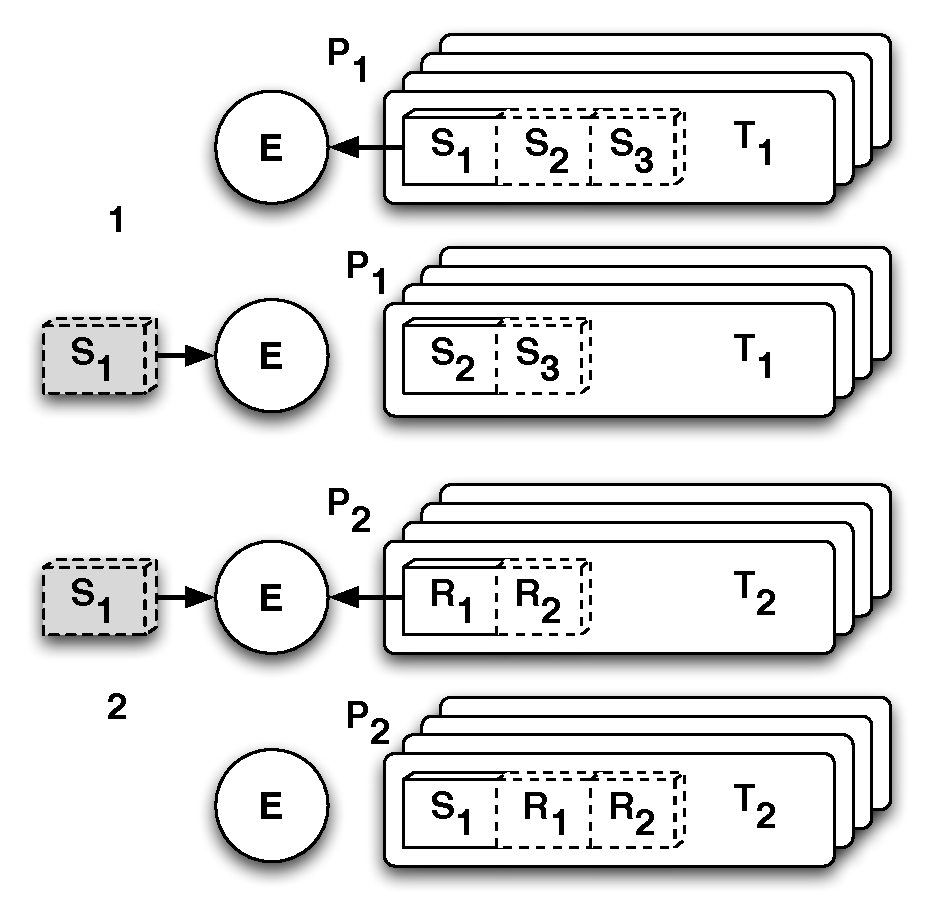
\includegraphics[scale=0.5]{Figures/communication.pdf}
\end{center}
\caption{Blocking and unblocking of parasitic threads.}
\label{fig:block_unblock}
\end{figure}

Figure~\ref{fig:block_unblock} shows the steps involved in a parasitic
communication, or blocking event, and we illustrate the interaction between the
parasitic threads and their hosts. The host threads are depicted as rounded
rectangles, parasitic threads are represented as blocks within their hosts, and
each processor as a queue of host threads. The parasite that is currently
executing on a given host and its stack is represented as a block with solid
edges; other parasites are represented as blocks with dotted edges. Reified
parasites are represented as shaded blocks. Host threads can be viewed as a
collection of parasitic threads all executing within the same stack space. When
a host thread is initially created it contains one such computation, namely the
expression it was given to evaluate when it was spawned.

Initially, the parasite \cf{$S_1$} performs a blocking action on a channel or
event, abstractly depicted as a circle. Hence, \cf{$S_1$} blocks and is
reified. The thread \cf{$T_1$} that hosted \cf{$S_1$} continues execution by
switching to the next parasite \cf{$S_2$}. \cf{$S_1$} becomes runnable when it
is unblocked. Part 2 of the figure shows the parasite \cf{$R_1$} on the thread
\cf{$T_2$} invoking an unblocking action. This unblocks \cf{$S_1$} and
schedules it on top of \cf{$R_1$}. Thus, the parasitic threads implicitly
migrate to the point of synchronization.

Further details aout parasitic threads including its operational semantics and
mapping of \acml primitives to parasitic threads can be found in~\cite{JFP14}.

\subsection{Garbage collector}

\MM garbage collector (GC) is optimized for throughput. It uses a single,
contiguous heap, shared among all the cores, with support for local allocation
and stop-the-world collection. In order to allow local allocation, each core
requests a page-sized chunk from the heap. While a single lock protects the
chunk allocation, objects are allocated within chunks by bumping a core-local
heap frontier.

In order to perform garbage collection, all the cores synchronize on a barrier,
with one core responsible for collecting the entire heap. The garbage
collection algorithm is inspired from Sansom's~\cite{Sansom91} collector, which
combines Cheney's two-space copying collector and Jonker's single-space sliding
compaction collector. Cheney's copying collector walks the live objects in the
heap just once per collection, while Jonker's mark-compact collector performs
two walks. But Cheney's collector can only utilize half of memory allocated for
the heap. Sansom's collector combines the best of both worlds. Copying
collection is performed when heap requirements are less than half of the
available memory. The runtime system dynamically switches to mark-compact
collection if the heap utilization increases beyond half of the available
space.

Since ML programs tend to have a high rate of allocation, and most objects are
short-lived temporaries, it is beneficial to perform generational collection.
The garbage collector supports Appel-style generational
collection~\cite{Appel89} for collecting temporaries. The generational
collector has two generations, and all objects that survive a generational
collection are copied to the older generation. Generational collection can work
with both copying and mark-compact major collection schemes.

\MM enables its generational collector only when it is profitable, which is
determined by the following heuristic. At the end of a major collection, the
runtime system calculates the ratio of live bytes to the total heap size. If
this ratio falls below a certain (tunable) threshold, then generational
collection is enabled for subsequent collections. By default, this ratio is
0.25.

\newcommand{\lc}{LC\xspace}
\newcommand{\prc}{PRC\xspace}
\newcommand{\smc}{SMC\xspace}
\newcommand{\kcore}{k_{core}}
\newcommand{\kmesh}{k_{mesh}}
\newcommand{\kram}{k_{ram}}

\lstset{
language=C,
numbers=left,
numberstyle=\footnotesize,
frame=single}

\lstset{deletekeywords={bool,int}}
\lstset{morekeywords={foreach,in}}

\lstset{classoffset=1, morekeywords={ZERO,ONE,LOCAL\_MANY,GLOBAL,FORWARDED},keywordstyle=\color{Red},
        classoffset=2, morekeywords={pointer,bool,int,Val,Ref,ThreadID,Thread,Set},keywordstyle=\color{OliveGreen}, %Types
        classoffset=0}% restore default


\chapter{\MMSCC: A Coherent and Managed Runtime for ML on the SCC}
\label{chap:aneris}

In this chapter, we describe \MMSCC, an extension of \MM that provides a
coherent address space on the SCC, optimizing for the SCC's memory hierarchy.
We begin with a \emph{local collector}\footnote{Other terms have been used in
the literature to indicate similar heap designs, notably private nursery, local
heap collector, thread-local or thread-specific heap, and on-the-fly
collection.} (\lc) design~\cite{Steele75, Doligez93, Steensgaard00, Anderson10,
Marlow11, Auhagen11} that partitions the heap into local heaps on each core and
a shared heap for cross-core communication. However, we observe that the cost
of memory barriers utilized in preserving the heap invariants have significant
costs. To eliminate theses costs, we propose a new GC design (\prc) that
utilizes the ample concurrency offered by our programming model combined with a
dynamic shape analysis to eliminate some of the GC overheads. This naturally
leads to a GC design that focuses on \emph{procrastination}~\cite{mmgc},
delaying writes that would necessitate establishing forwarding pointers until a
GC, where there is no longer a need for such pointers. The GC leverages the
mostly functional nature of ACML programs and a new object property called
\emph{cleanliness}, which enables a broad class of objects to be moved from a
local to a shared heap without requiring a full traversal of the local heap to
fix existing references; cleanliness enables an important optimization that
achieves the effect of procrastination without actually having to initiate a
thread stall. Our final design (\smc) integrates SCC's support for
software-managed cache coherence (SMC)~\cite{SMC} into the extant memory
barriers to improve the design further.

We begin by discussing in detail the architecture and programming model of the
SCC, which serves as our prototype non cache coherent architecture. However,
the use of SCC by no means restricts the applicability of our ideas to other
scalable manycore architectures~\cite{mmgc}. Then, we present the three GC
designs. Finally, we present a comprehensive evaluation of the three designs.

\section{The Intel Single-chip Cloud Computer}

\begin{figure}[t]
\begin{center}
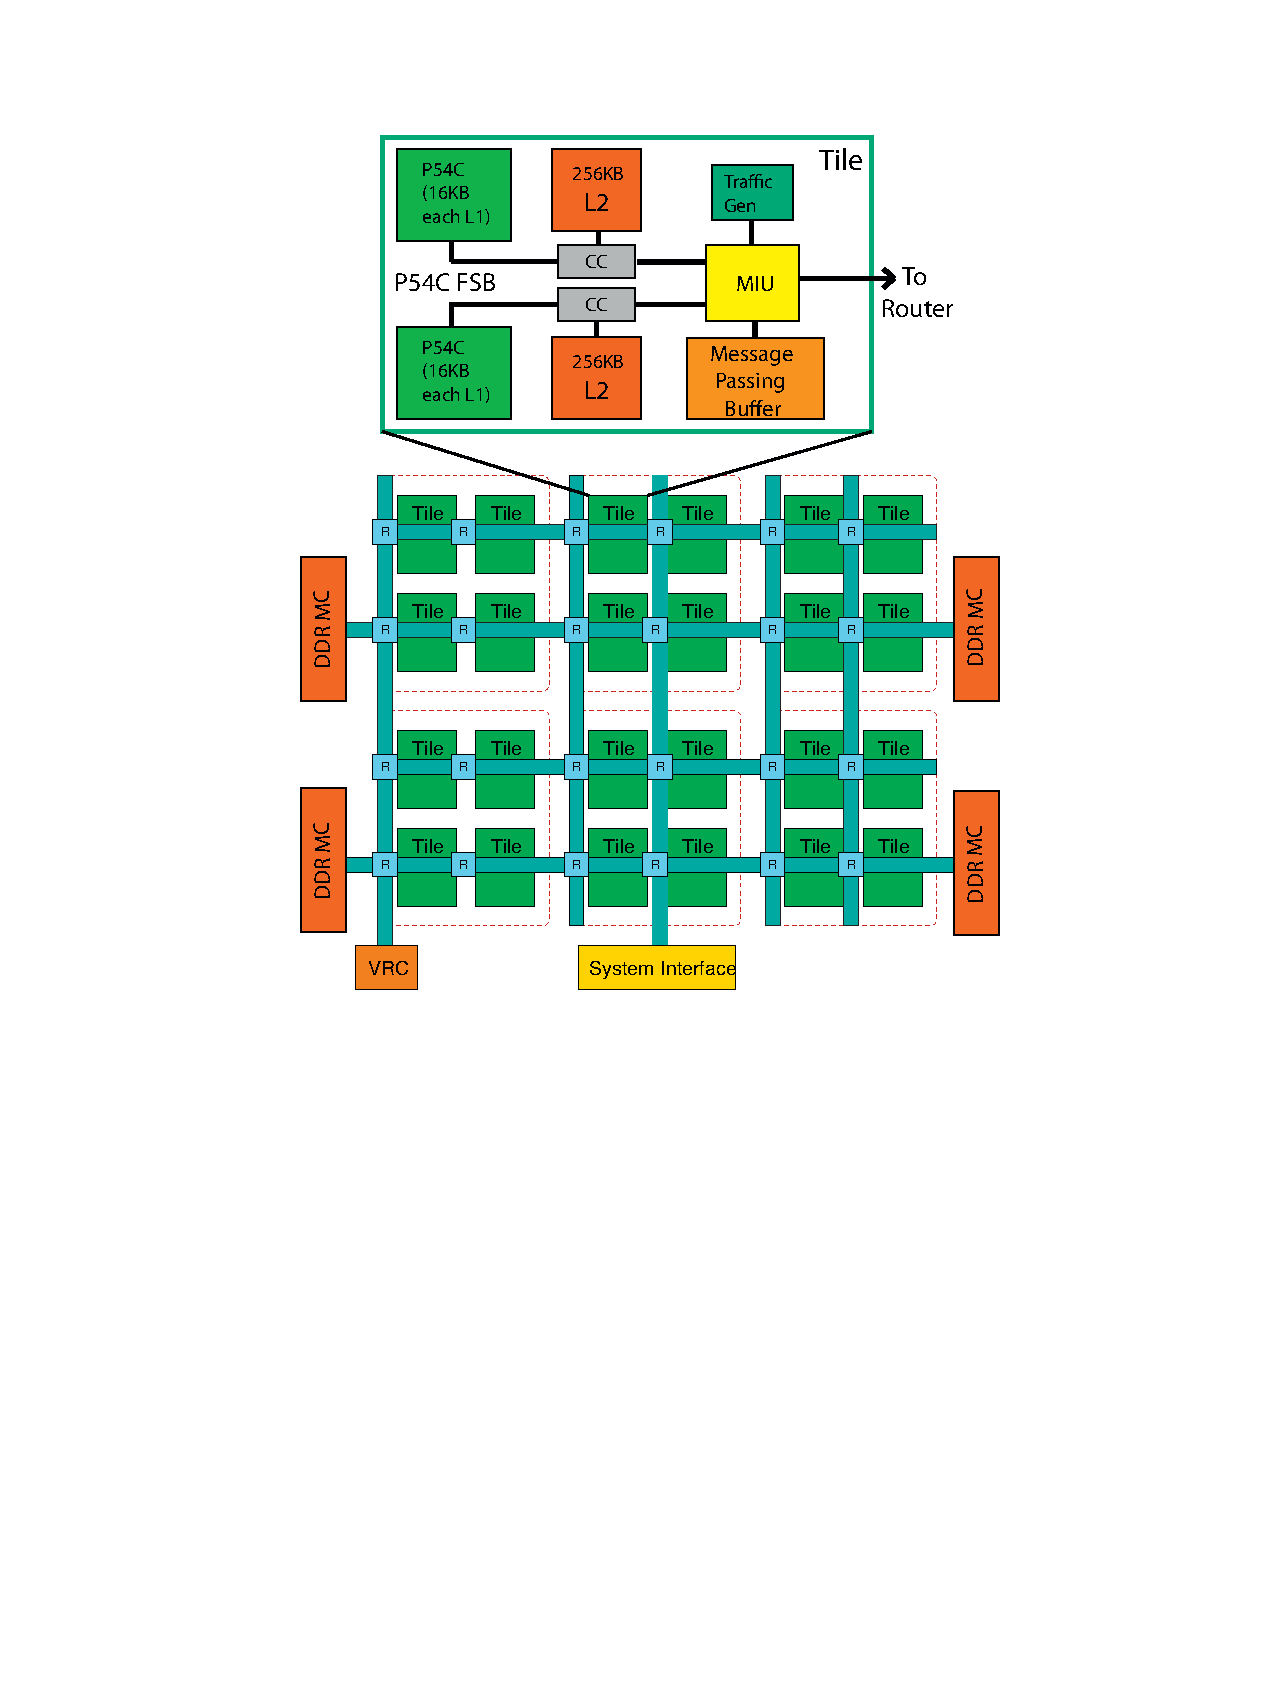
\includegraphics{Figures/SCC.pdf}
\end{center}
\caption{The architecture of the Intel SCC processor}
\label{fig:scc}
\end{figure}

Intel SCC~\cite{Mattson2010} (Figure~\ref{fig:scc}) is a many-core processor
with 48 P54C cores on a single chip, grouped as 24 tiles, organized in a 4
$\times$ 6 mesh network with a bisection bandwidth of 256 Gb/s. The most
interesting aspect of the SCC architecture is the complete lack of cache
coherence between the cores, and the presence of fast on-die message-passing
network interface. The 24 tiles on the chip are divided into 4 quadrants, and
each quadrant is connected to a DDR3 memory controller. Each core has 16KB of
private L1 instruction and data caches, and 256 KB of L2 cache shared with the
other core on the same tile.

In addition, each tile has a 16KB message-passing buffer (MPB) used for
message-passing between the cores. The message passing buffers are the only
caches that are accessible across all of the cores. The data used in on-chip
communication is read from MPB, cached in L1 cache, but bypasses the L2 cache.
The cache uses no-allocate policy on writes, and L1 cache incorporates a
write-combine buffer. According to the processor
specifications~\cite{Mattson2010}, the read latencies in this architecture are:
\begin{mathpar}
\begin{array}{rcl}
\textrm{LocalMPB} & = & 45~\kcore + 8~\kmesh \\
\textrm{RemoteMPB} & = & 45~\kcore + 4*n*2~\kmesh \\
\textrm{DRAM} & = & 40~\kcore + 4*n*2~\kmesh + 46~\kram
\end{array}
\end{mathpar}

\noindent where $\kcore$, $\kmesh$ and $\kram$ are the cycles of core, mesh
network and memory respectively. In our experimental setup, where 6 tiles share
a memory controller, the number of hops n to the memory controller could be $0
< n \le 8$. Hence, the DRAM accesses are far more expensive than the MPBs. Each
core additionally has a test and set register that is accessible from all other
cores. The SCC uses 32-bit Pentium cores. A programmable, software-managed
Look-Up Table (LUT) provides a means for implementing hybrid private and shared
address spaces in the system.

\subsection{Software System}

From the programmer's point of view, SCC resembles a cluster of nodes, with
portions of memory shared between the cores. Each core runs a linux kernel
image, and does not share any operating system services with the other cores.
Since SCC does not provide hardware cache coherence, it provides software
support for managing coherence. First, SCC provides support for tagging a
specific virtual address space as shared across all of the cores. Caching can
also be selectively enabled on this address space; SCC tags this address space
as having message passing buffer type (MPBT).

Data typed as MPBT bypass L2 and go directly to L1. SCC also provides a
special, 1-cycle instruction called \cf{CL1INVMB} that marks all data of type
MPBT as invalid L1 lines. In addition, the usual \cf{WBINVD} instruction can be
used to flush and invalidate the L1 cache. Since the cores use write-combine
buffers, a correct flushing procedure should also flush the write-combine
buffers. SCC does not provide primitive support for this purpose, but
write-combine buffers can easily be flushed in software by performing a series
of dummy writes to distinct memory locations, which fills the buffer and
flushes any previous writes.

Typically, a programmer works with release consistency in order to utilize
cached shared virtual memory. The SMC~\cite{SMC} library provides
\cf{smcAcquire()} to fetch changes from other cores (invalidates MPBT cache
lines in L1 cache) and issues \cf{smcRelease()} to publish its updates (flushes
the L1 cache, if the cache is operating in write back mode, and flushes the
write-combine buffers).

SCC's software stack also includes cross-core message-passing libraries
implemented over the MPBs, including RCCE~\cite{Mattson2010} and
RCKMPI~\cite{Urena2011}. RCCE is optimized for Single Program Multiple Data
(SPMD) parallel programming model, where the program is structured in such a
way that the sender and the receiver ideally arrive at the communication point
at the same time. The sender writes the message to the MPB, while the receiver
busy waits (invalidating its cache every iteration to fetch recent writes),
waiting for a special flag value to be written along with the message. After
the sender writes the flag, the receiver reads the message into its private
memory, while the sender busy waits (also invalidating its cache every
iteration). Finally, the receiver writes a completion flag, which concludes the
message transfer.

It is worthwhile pointing out that RCCE uses just the MPBs, while RCKMPI uses
MPBs for small messages (less than 8KB --- the maximum message size that would
fully fit in the MPB) and the DRAM for larger messages. Despite having a higher
bandwidth and lower latency, the synchronization costs involved in transferring
a large multi-part message over the MPB outweighs the benefits.

\section{Local Collector (\lc)}
\label{sec:lc}

Splitting a program heap among a set of cores is a useful technique to exploit
available parallelism on scalable multicore platforms: each core can allocate,
collect, and access data locally, moving objects to a global, shared heap only
when they are accessed by threads executing on different cores. This design
allows local heaps to be collected independently, with coordination required
only for global heap collection. In contrast, stop-the-world collectors need a
global synchronization for every collection.

\subsection{Heap Architecture}

\begin{figure}[t]
\centering
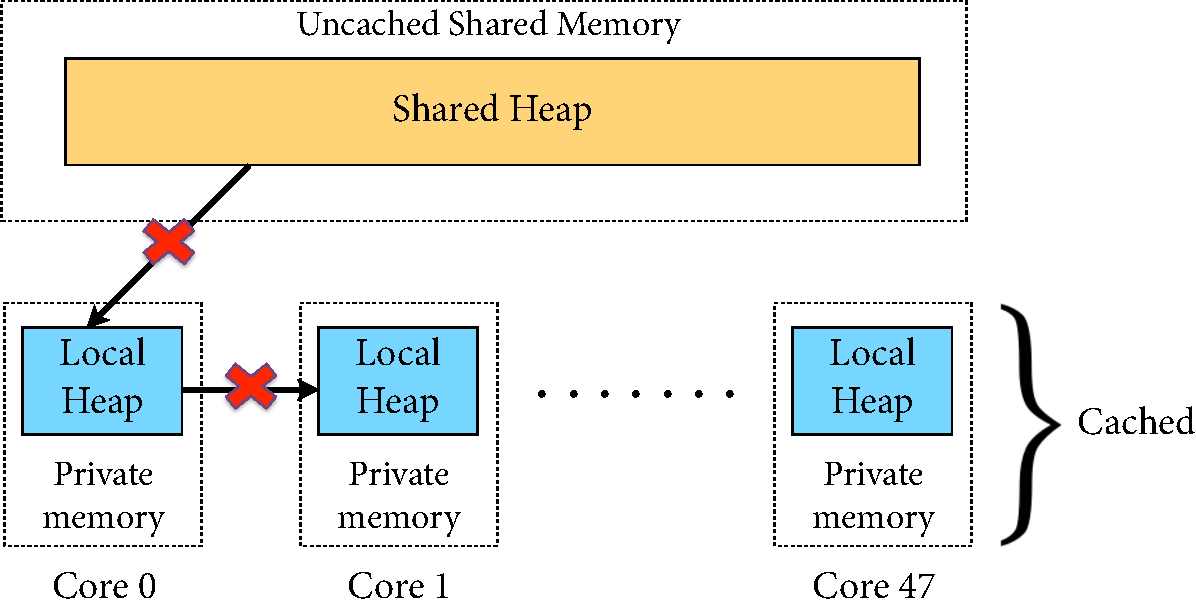
\includegraphics[width=0.8\textwidth]{Figures/LocalCollector.pdf}
\caption{Local collector heap organization for the SCC}
\label{fig:lc}
\end{figure}


Our local collector design for the SCC is shown in Figure~\ref{fig:lc}. The key
idea here is that the local heaps are allocated in each of the cores
\emph{cached} private memory, into which new objects are allocated by default.
The private heaps are allocated on the memory banks closest to the core to
optimize for the memory hierarchy and reduce mesh congestion. Since the design
allows independent collection of local heaps, the design can scale to hundreds
of cores~\cite{JFP14}, and benefits cache coherent architectures as well. The
shared heap is allocated in the shared memory, and visible to all of the cores.
In order to circumvent the coherence issues, we disable caching on the shared
heap. Hence, every shared memory access goes to the DRAM. The shared heap pages
are interleaved across all of the memory banks to uniformly spread the
requests.

\subsection{Heap Invariants}

In order to ensure that cores cannot directly or indirectly access objects on
other local heaps, which would complicate the ability to perform independent
local heap collection, the following invariants need to be preserved:

\begin{itemize}
\item No pointers are allowed from one core's local heap to another.
\item No pointers are permitted from the shared heap to the local heap.
\end{itemize}

\noindent Both invariants are necessary to perform independent local
collections.  The reason for the first is obvious.  The second invariant
prohibits a local heap from transitively accessing another local heap object
via the shared heap.  In order to preserve these invariants, the mutator
typically executes a \emph{write barrier} on every store operation. The write
barrier ensures that before assigning a local object reference (source) to a
shared heap object (target), the local object along with its transitive object
closure is lifted to the shared heap. We call such writes \emph{globalizing
writes} as they export information out of local heaps.  The execution of the
write barrier creates \emph{forwarding pointers} in the original location of
the lifted objects in the local heap. These point to the new locations of the
lifted objects in the shared heap. Since objects can be lifted to the shared
heap on potentially any write, the mutator needs to execute a \emph{read
barrier} on potentially every read. The read barrier checks whether the object
being read is the actual object or a forwarding pointer, and in the latter
case, indirects to the object found on the shared heap.  Forwarding pointers
are eventually eliminated during local collection.

\subsection{Allocation and Collection}

The allocations in the shared heap is performed similar to allocations in the
stop-the-world collector, where each core allocates a page-sized chunk in the
shared heap and performs object allocation by bumping its core-local shared
heap frontier. Allocations in the local heaps do not require any
synchronization. Garbage collection in the local heaps is similar to the
baseline collector, except that it crucially does not require global
synchronization.

Objects are allocated in the shared heap only if they are to be shared between
two or more cores. Objects are automatically lifted to the shared heap because
of globalizing writes and spawning a thread on a different core. Apart from
these, all globals are allocated in the shared heap, since globals are visible
to all cores by definition. Thus, for the ML programmer on this system, the
absence of cache coherence is completely hidden, the SCC appears as a cache
coherent multicore machine.

For a shared heap collection, all of the cores synchronize on a barrier and
then a single core collects the heap. Along with globals, all the live
references from local heaps to the shared heap are considered to be roots for a
shared heap collection. In order to eliminate roots from dead local heap
objects, before a shared heap collection, local collections are performed on
each core to eliminate such references.

The shared heap is also collected using Sansom's dual-mode garbage collector.
However, we do not perform generational collection on the shared heap. This is
because of two reasons. First, objects in the shared heap, shared between two
or more cores, are expected to live longer than a typical object collected
during generational collection. Secondly, shared heap collection requires
global synchronization, and it is wise to perform such collections rarely.

\subsection{Remembered Stacks}
\label{sec:aneris_rem_stack}

In \MM threads can synchronously or asynchronously communicate with each other
over first-class message-passing communication channels. If a receiver is not
available, a sender thread, or in the case of asynchronous communication the
implicitly created thread, can block on a channel. If the channel resides in
the shared heap, the thread object, its associated stack and the transitive
closure of all objects reachable from it on the heap would be lifted to the
shared heap as part of the blocking action. Since channel communication is the
primary mode of thread interaction in our system, we would quickly find that
most local heap objects end up being lifted to the shared heap. This would be
highly undesirable.

Hence, we choose never to move stacks to the shared heap. We add an exception
to our heap invariants to allow thread $\rightarrow$ stack pointers, where the
thread resides on the shared heap, and references a stack object found on the
local heap. Whenever a thread object is lifted to the shared heap, a reference
to the corresponding stack object is added to the set of remembered stacks.
This remembered set is considered as a root for a local collection to enable
tracing of remembered stacks.

Before a shared heap collection, the remembered set is cleared; only those
stacks that are reachable from other GC roots survive the shared heap
collection. After a shared heap collection, the remembered set of each core is
recalculated such that it contains only those stacks, whose corresponding
thread objects reside in the shared heap, and have survived the shared heap
collection.

Remembered stacks prevent thread local objects from being lifted to the shared
heap, but require breaking the heap invariant to allow a thread object in the
shared heap to refer to a stack object on the local heap. This relaxation of
heap invariant is safe. The only object that can refer to thread-local stacks
is the corresponding thread object. The thread objects are completely managed
by the scheduler, and are not exposed to the programmer. As a result, while the
local heap objects can point to a shared-heap thread object, whose stack might
be located on a different local heap, the only core that can modify such a
stack (by running the thread) is the core that owns the heap in which the stack
is located. Thus, there is no possibility of direct references between local
heaps. Hence, the remembered stack strategy is safe with respect to garbage
collection.

\subsection{Read Barrier and Overheads}

In a mostly functional language like Standard ML, the number of reads are far
likely to outweigh the number of mutations. Because of this fact, the aggregate
cost of read barriers can be both substantial and vary dramatically based on
underlying architecture characteristics~\cite{Blackburn04}. To this end, we
describe our read barrier design, and the cost/benefit of read barriers in our
system.

\subsubsection{Read Barrier Design}

\begin{figure}[t]
\begin{lstlisting}
pointer readBarrier (pointer p) {
  if (!isPointer(p)) return p;
  if (getHeader(p) == FORWARDED)
    return *(pointer*)p;
  return p;
}
\end{lstlisting}
\caption{Read barrier.}
\label{code:read_barrier}
\end{figure}

Figure~\ref{code:read_barrier} shows the pseudo-C code for our read barrier.
Whenever an object is lifted to the shared heap, the original object's header
is set to \cf{FORWARDED}, and the first word of the object is overwritten with
the new location of the object in the shared heap. Before an object is read,
the mutator checks whether the object has been forwarded, and if it is, returns
the new location of the object. Hence, our read barriers are
conditional~\cite{Blackburn04,Baker}.

MLton represents non-value carrying constructors of (sum) datatypes using
non-pointer values. If such a type additionally happens to have value-carrying
constructors that reference heap-allocated objects, the non-pointer value
representing the empty constructor will be stored in the object pointer field.
Hence, the read barrier must first check whether the presumed pointer does in
fact point to a heap object.  Otherwise, the original value is returned (line
2). If the given pointer points to a forwarded object, the current location of
the object in the shared heap is returned. Otherwise, the original value is
returned.

While our read barrier implementation is conditional~\cite{Baker}, there exist
unconditional variants~\cite{Brooks84}, where all loads unconditionally forward
a pointer in the object header to get to the object. For objects that are not
forwarded, this pointer points to the object itself. Although an unconditional
read barrier, would have avoided the cost of the second branch in our read
barrier implementation, it would necessitate having an additional address
length field in the object header for an indirection pointer.

Most objects in our system tend to be small. In our benchmarks, we observed
that 95\% of the objects allocated were less than 3 words in size, including a
word-sized header. The addition of an extra word in the object header for an
indirection pointer would lead to substantial memory overheads, which in turn
leads to additional garbage collection costs. Moreover, trading branches with
loads is not a clear optimization as modern processors allow speculation
through multiple branches, especially ones that are infrequent. Hence, we
choose to encode read barriers conditionally rather than unconditionally.

In addition, \MM performs a series of optimizations to minimize heap
allocation, thus reducing the set of read barriers actually generated.  For
example, references and arrays that do not escape out of a function are
flattened.  Combined with aggressive inlining and simplification optimizations
enabled by whole-program compilation, object allocation on the heap can be
substantially reduced.

The compiler and runtime system ensure that entries on thread stacks never
point to a forwarded object. Whenever an object pointer is stored into a
register or the stack, a read barrier is executed on the object pointer to get
the current location of the object. Immediately after an globalizing write or a
context switch, the current stack is walked and references to forwarded objects
are updated to point to the new location of lifted objects in the shared heap.
Additionally, before performing an globalizing write, register values are saved
on the stack, and reloaded after exit. Thus, as a part of fixing references to
forwarding pointers from the stack, references from registers are also fixed.
This ensures that the registers never point to forwarded objects either. Hence,
no read barriers are required for dereferencing object pointers from the stack
or registers. This optimization is analogous to ``eager" read barriers as
described in~\cite{Bacon03}. Eager read barrier elimination has marked
location is loaded into a register, but all further accesses can elide
executing the barrier.

\subsubsection{Evaluation}

\begin{figure}[t]
  \centering
  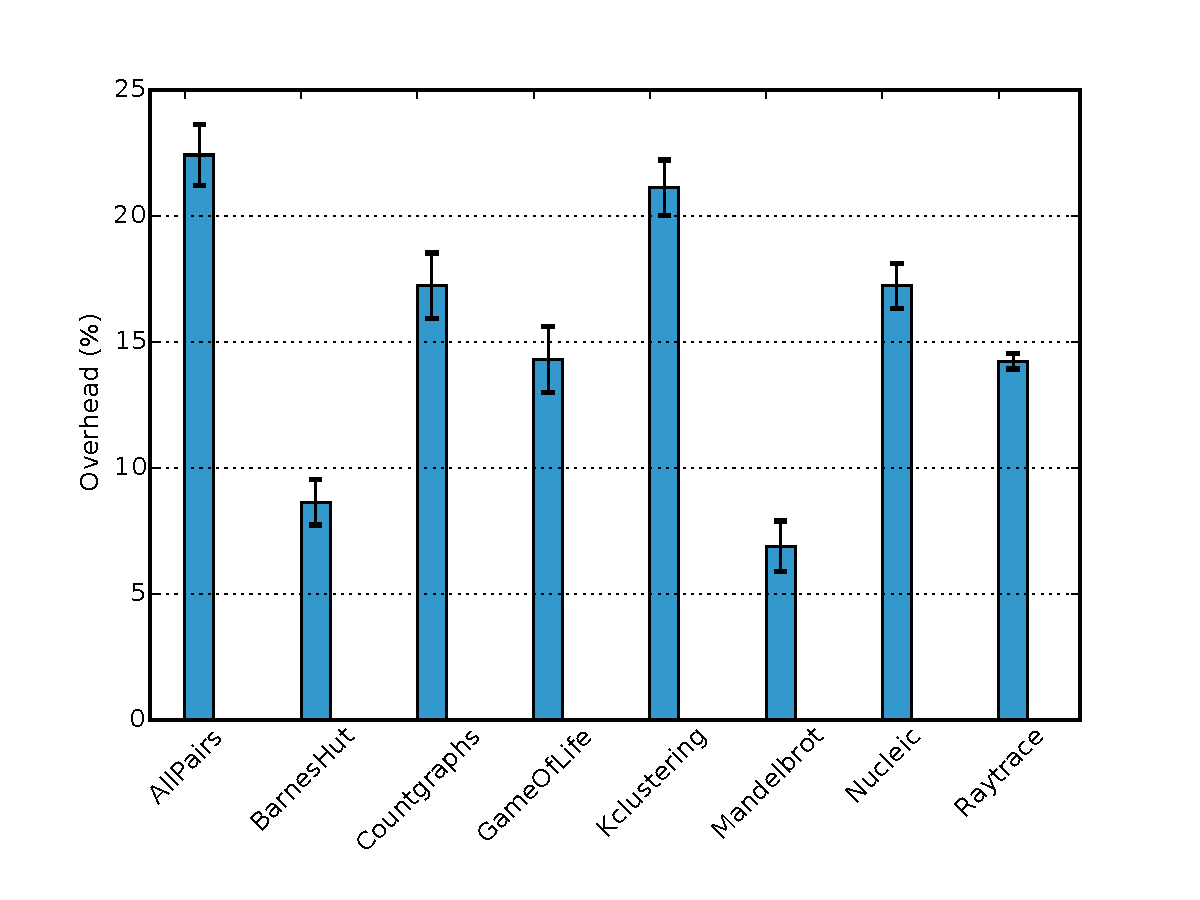
\includegraphics[width=0.9\textwidth]{Graphs/RB_overhead}
	\caption{Read barrier overhead as a percentage of mutator time.}
  \label{fig:rb-overhead}
\end{figure}

We evaluated a set of 8 benchmarks (described in Section~\ref{sec:gc_bench})
each running on all 48 cores on the SCC to measure read barrier overheads.
Figure~\ref{fig:rb-overhead} shows these overheads as a percentage of mutator
time. Our experiments reveal that, on average, the mutator spends 15.3\% of the
time executing read barriers for our benchmarks.

\begin{table}[t]
\begin{center}
\caption{Effectiveness of read barrier checks: RB invocations represents the
average number of read barrier invocations and forwarded represents the average
number of instances when the read barrier encountered a forwarded object.}
\label{tab:rb_utility}
\begin{tabular} {|l|r|r|}
\hline
{\bf Benchmark} & {\bf RB invocations ($\times 10^6$)} & {\bf Forwarded}\\
\hline
{AllPairs} & 9,753 \ci{431} & 123 \ci{11} \\
{BarnesHut} & 2,864 \ci{176} & 52,702 \ci{1830} \\
{CountGraphs} & 2,584 \ci{119} & 0 \ci{0} \\
{GameOfLife} & 4,858 \ci{276} & 2,143 \ci{43}\\
{KClustering} & 3,780 \ci{265} & 101 \ci{7} \\
{Mandelbrot} & 2,980 \ci{79} & 23 \ci{3} \\
{Nucleic} & 2,887 \ci{135} & 328 \ci{21} \\
{Raytrace} & 2,217 \ci{90} & 0 \ci{0}\\
\hline
\end{tabular}
\end{center}
\end{table}

The next question to ask is whether the utility of the read barrier justifies
its cost. To answer this question, we measure the number of instances the read
barrier is invoked and the number of instances the barrier finds a forwarded
object (see Table~\ref{tab:rb_utility}).  We see that read barriers find
forwarded objects in less than one thousandth of a percent of the number of
instances they are invoked. Thus, in our system, the cost of read barriers is
substantial, but only rarely do they have to perform the task of forwarding
references. These results motivate our interest in a memory management design
that eliminates read barriers altogether.

\section{Procrastinating Collector (\prc)}

Eliminating read barriers, however, is non-trivial. Abstractly, one can avoid
read barriers by eagerly \emph{fixing} all references that point to forwarded
objects at the time the object is lifted to the shared heap, ensuring the
mutator will never encounter a forwarded object. Unfortunately, this requires
being able to enumerate all the references that point to the lifted object; in
general, gathering this information is very expensive as the references to an
object might originate from any object in the local heap.

We consider an alternative design that completely eliminates the need for read
barriers \emph{without} requiring a full scan of the local heap whenever an
object is lifted to the shared heap.  The design is based on the observation
that read barriers can be clearly eliminated if forwarding pointers are never
introduced.  One way to avoid introducing forwarding pointers is to
\emph{delay} operations that create them until a local garbage collection is
triggered.  In other words, rather than executing a store operation that would
trigger lifting a thread local object to the shared heap, we can simply
\emph{procrastinate}, thereby stalling the thread that needs to perform the
store.  The garbage collector must simply be informed of the need to lift the
object's closure during its next local collection. After collection is
complete, the store can take place with the source object lifted, and all
extant heap references properly adjusted.  As long as there is sufficient
concurrency to utilize existing computational resources, in the form of
available runnable threads to run other computations, the cost of
procrastination is just proportional to the cost of a context switch.

Moreover, it is not necessary to always stall an operation that involves
lifting an object to the shared heap.  We consider a new property for objects
(and their transitive object closures) called \emph{cleanliness}.  A clean
object is one that can be safely lifted to the shared heap without introducing
forwarding pointers that might be subsequently encountered by the mutator:
objects that are immutable, objects only referenced from the stack, or objects
whose set of incoming heap references is known, are obvious examples.  The
runtime analysis for cleanliness is combined with a specialized write barrier
to amortize its cost.  Thus, procrastination provides a general technique to
eliminate read barriers, while cleanliness serves as an important optimization
that avoids stalling threads unnecessarily.

The effectiveness of our approach depends on a programming model in which (a)
most objects are clean, (b) the transitive closure of the object being lifted
rarely has pointers to it from other heap allocated objects, and (c) there is a
sufficient degree of concurrency in the form of runnable threads; this avoids
idling available cores whenever a thread is stalled performing an globalizing
write that involves an unclean object.  We observe that conditions (a) and (b)
are common to functional programming languages and condition (c) follows from
the \acml\ runtime model. Our technique does not rely on programmer
annotations, static analysis or compiler optimizations to eliminate read
barriers, and can be completely implemented as a lightweight runtime technique.

\subsection{Cleanliness Analysis}
\label{sec:clean}

Although \acml provides an abundance of concurrency, with the procrastination
mechanism, many of the threads in a program may end up blocked on globalizing
writes, waiting for a local garbage collection to unblock them. If all of the
threads on a particular core have procrastinated, then a local garbage
collection is needed in order to make progress. Such \emph{forced} local
garbage collections make the program run longer, and hence subdue the benefit
of eliminating read barriers. Hence, it is desirable to avoid procrastination
whenever possible.

In this section, we describe our cleanliness analysis, which identifies objects
on which globalizing writes do not need to be stalled. We first present auxiliary
definitions that will be utilized by cleanliness checks, and then describe the
analysis.

\subsubsection{Heap Session}

Objects are allocated in the local heap by bumping the local heap frontier. In
addition, associated with each local heap is a pointer called \cf{sessionStart}
that always points to a location between the start of the heap and the
frontier. This pointer introduces the idea of a \emph{heap session}, to capture
the notion of recently allocated objects. Every local heap has exactly two
sessions: a \emph{current session} between the \cf{sessionStart} and the heap
frontier and a \emph{previous session} between the start of the heap and
\cf{sessionStart}. Heap sessions are used by the cleanliness analysis to limit
the range of heap locations that need to be scanned to test an object
closure\footnote{In the following, we write \emph{object closure} to mean the
set of objects reachable from some root on the heap; to avoid confusion, we
write \emph{function closure} to mean the representation of an SML function as
a pair of function code pointer and static environment.} for cleanliness.
Assigning the current local heap frontier to the \cf{sessionStart} pointer
starts a new session. We start a new session on a context switch, a local
garbage collection and after an object has been lifted to the shared heap.

\subsubsection{Reference Count}

We introduce a limited reference counting mechanism for local heap objects that
counts the number of references from other local heap objects. Importantly, we
do not consider references from ML thread stacks. The reference count is
meaningful only for objects reachable in the current session. For such objects,
the number of references to an object can be one of four values: \cf{ZERO},
\cf{ONE}, \cf{LOCAL\_MANY}, and \cf{GLOBAL}. We steal 2 bits from the object
header to record this information. A reference count of \cf{ZERO} indicates
that the object only has references from registers or stacks, while an object
with a count of \cf{ONE} has exactly one pointer from the current session. A
count of \cf{LOCAL\_MANY} indicates that this object has more than one
reference, but that all of these references originate from the current session.
\cf{GLOBAL} indicates that the object has at least one reference that
originates from outside the current session.

\begin{figure}[t]
\centering
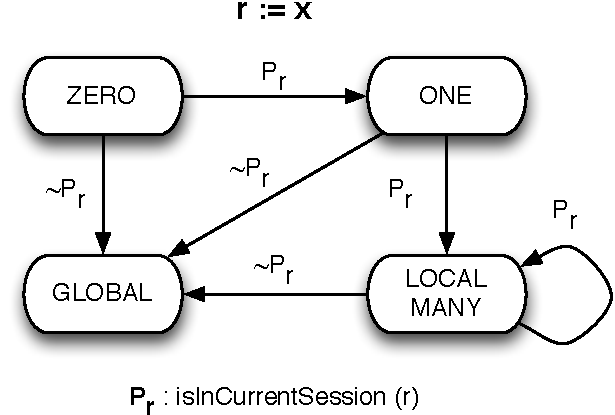
\includegraphics[width=0.5\textwidth]{Figures/std_reference_count}
\caption{State transition diagram detailing the behavior of the reference
counting mechanism with respect to object \cf{x} involved in an assignment,
\cf{r := x}, where \cf{P}$_\textrm{\cf{r}}$ = \cf{isInCurrentSession(r)}.}
\label{fig:std_ref_count}
\end{figure}

The reference counting mechanism is implemented as a part of the write barrier
(Lines 13--22 in Figure~\ref{code:writeBarrier}).
Figure~\ref{fig:std_ref_count} illustrates the state transition diagram for the
reference counting mechanism. Observe that reference counts are non-decreasing.
Hence, the reference count of any object represents the maximum number of
references that pointed to the object at any point in its lifetime.

\subsubsection{Cleanliness}

An object closure is said to be clean, if for each object reachable from the
root of the object closure,

\begin{itemize}
\item the object is immutable or in the shared heap. Or,
\item the object is the root, and has \cf{ZERO} references. Or,
\item the object is not the root, and has \cf{ONE} reference. Or,
\item the object is not the root, has \cf{LOCAL\_MANY} references, and is in the
current session.
\end{itemize}

\noindent Otherwise, the object closure is not clean.

\begin{figure}[t]
\begin{lstlisting}
bool isClean (pointer p, bool* isLocalMany) {
  clean = true;
  foreach o in reachable(p) {
    if (!isMutable(o) || isInSharedHeap(o))
      continue;
    nv = getRefCount(o);
    if (nv == ZERO)
      clean &&= true;
    else if (nv == ONE)
      clean &&= (o != p);
    else if (nv == LOCAL_MANY) {
      clean &&= (isInCurrentSession(o));
      *isLocalMany = true;
    }
    else
      clean = false;
  }
  return clean;
}
\end{lstlisting}
\caption{Cleanliness check.}
\label{code:cleanliness}
\end{figure}

Figure~\ref{code:cleanliness} shows an implementation of an object closure
cleanliness check. Since the cleanliness check, memory barriers, and the
garbage collector are implemented in low-level code (C, assembly and low-level
intermediate language in the compiler), this code snippet, and others that
follow in this section are in pseudo-C language, to better represent their
implementation. If the source of an globalizing assignment is immutable, we can
make a copy of the immutable object in the shared heap, and avoid introducing
references to forwarded objects. Standard ML does not allow the programmer to
test the referential equality of immutable objects. Equality of immutable
objects is always computed by structure. Hence, it is safe to replicate
immutable objects. If the object is already in the shared heap, there is no
need to move this object.

\begin{figure}[t]
\centering
\subfigure[Tree-structured object closure]{\label{fig:cleanliness_tree}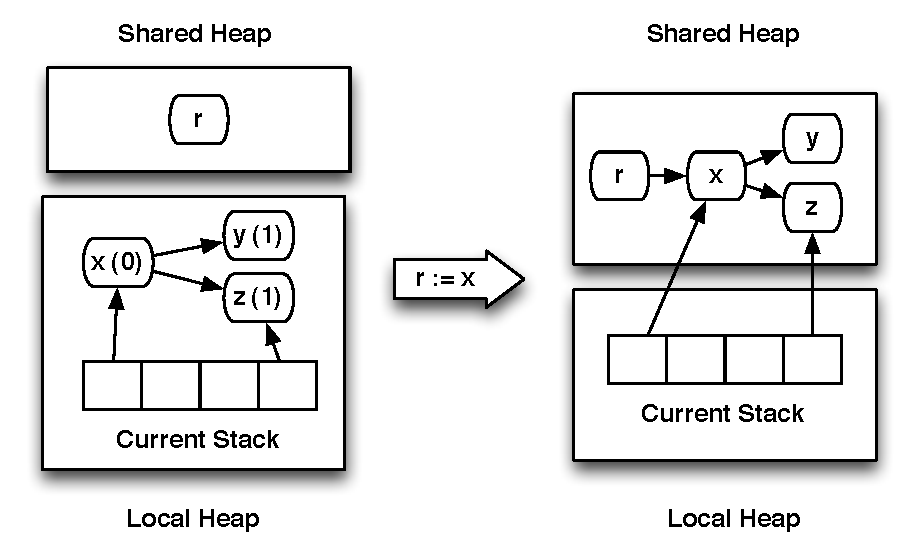
\includegraphics[width=0.7\textwidth]{Figures/Cleanliness_Tree}}\\
\subfigure[Session-based cleanliness]{\label{fig:cleanliness_session}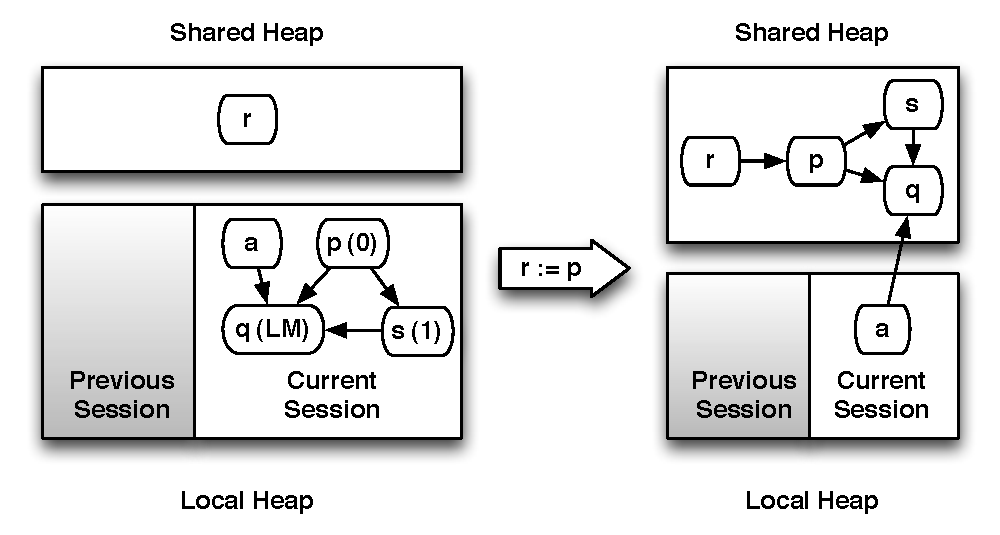
\includegraphics[width=0.7\textwidth]{Figures/Cleanliness_Session}}
\caption{Utilizing object closure cleanliness information for globalizing writes to avoid references to forwarded objects.}
\label{fig:cleanliness_examples}
\end{figure}

If the object closure of the source of a globalizing write is clean, we can move
the object closure to the shared heap and quickly fix all of the forwarding
pointers that might be generated. For example, consider an object that defines
a tree structure; such an object is clean if the root has \cf{ZERO} references
and all of its internal nodes have \cf{ONE} reference from their parent.  A
root having \cf{ZERO} references means it is accessed only via the stack; if it
had a count of \cf{ONE}, the outstanding reference may emanate from the heap.
Internal nodes having a reference count of \cf{ONE} implies they are reachable
only via other nodes in the object being traced.
Figure~\ref{fig:cleanliness_tree} shows such an object closure. In this
example, we assume that all objects in the object closure are mutable. The
reference count of relevant nodes is given in the brackets.  Both the root and
internal nodes can have pointers from the current stack not tracked by the
reference count. After lifting the object closure, the references originating
from the current stack are fixed by walking the stack.

Object closures need not just be trees and can be arbitrary graphs, with
multiple incoming edges to a particular object in the object closure. How do we
determine if the incoming edges to an object originate from the object closure
or from outside the object closure (from the local heap)? We cannot answer this
question without walking the local heap. Hence, we simplify the question to
asking whether all the pointers to an object originate from the current
session. This question is answered in the affirmative if an object has a
reference count of \cf{LOCAL\_MANY} (lines 11--13 in
Figure~\ref{code:cleanliness}).

Figure~\ref{fig:cleanliness_session} shows an example of a object closure whose
objects have at most \cf{LOCAL\_MANY} references. Again, we assume that all
objects in the object closure are mutable. In the transitive object closure
rooted at \cf{p}, object \cf{q} has locally many references. These references
might originate from the object closure itself (edges \cf{p $\rightarrow$ q}
and \cf{s $\rightarrow$ q}) or from outside the object closure (edge \cf{a
$\rightarrow$ q}). After lifting such object closures to the shared heap, only
the current session is walked to fix all of the references to forwarded objects
created during the copy. In practice (Section~\ref{sec:impact_session}),
current session sizes are much smaller than heap sizes, and hence globalizing
writes can be performed quickly.

Finally, in the case of \cf{LOCAL\_MANY} references, the object closure is
clean, but unlike other cases, after lifting the object closure to the shared
heap, the current session must be walked to fix any references to forwarded
objects. This is indicated to the caller of \cf{isClean} function by assigning
\cf{true} to \cf{*isLocalMany}, and is used in the implementation of lifting an
object closure to the shared heap (Figure~\ref{code:lift}).

\subsection{Write Barrier}
\label{sec:write_barrier}

\begin{figure}[t]
\begin{lstlisting}
Val writeBarrier (Ref r, Val v) {
  if (isObjptr(v)) {
    //Lift if clean or procrastinate
    if (isInSharedHeap(r) &&
        isInLocalHeap(v)) {
      isLocalMany = false;
      if (isClean(v, &isLocalMany))
        v = lift(v, isLocalMany);
      else
        v = suspendTillGCAndLift(v);
    }
    //Tracking cleanliness
    if (isInLocalHeap (r) &&
        isInLocalHeap(v)) {
      n = getRefCount(v);
      if (!isInCurrentSession (r))
        setNumRefs(v, GLOBAL);
      else if (n == ZERO)
        setNumRefs(v, ONE);
      else if (n < GLOBAL)
        setNumRefs(v, LOCAL_MANY);
    }
  }
  return v;
}
\end{lstlisting}
\caption{Write barrier implementation.}
\label{code:writeBarrier}
\end{figure}

In this section, we present the modifications to the write barrier to eliminate
the possibility of creating references from reachable objects in the local heap
to a forwarded object. The implementation of our write barrier is presented in
Figure~\ref{code:writeBarrier}. A write barrier is invoked prior to a write and
returns a new value for the source of the write. The check \cf{isObjptr} at
line 2 returns true only for heap allocated objects, and is a compile time
check. Hence, for primitive valued writes, there is no write barrier. Lines 4
and 5 check whether the write is globalizing. If the source of the object is
clean, we lift the transitive object closure to the shared heap and return the
new location of the object in the shared heap.

\subsubsection{Delaying Writes}

If the source of an globalizing write is not clean, we suspend the current thread
and switch to another thread in our scheduler. The source of the write is added
to a queue of objects that are waiting to be lifted. Since the write is not
performed, no forwarded pointers are created. If programs have ample amounts of
concurrency, there will be other threads that are waiting to be run.  However,
if all threads on a given core are blocked on a write, we move all of the
object closures that are waiting to be lifted to the shared heap. We then force
a local garbage collection, which will, as a part of the collection, fix all of
the references to point to the new (lifted) location on the shared heap. Thus,
the mutator never encounters a reference to a forwarded object. \\

\subsubsection{Lifting Objects to the Shared Heap}

\begin{figure}[t]
\begin{lstlisting}
Set imSet;
void liftHelper (pointer* op, pointer* frontierP) {
  frontier = *frontierP;
  o = *op;
  if (isInSharedHeap(o)) return;
  copyObject (o, frontier);
  *op = frontier + headerSize(o);
  *frontierP = frontier + objectSize(o);
  if (isMutable(o)) { setHeader(o, FORWARDED); *o = *op; }
  else imSet += o;
}

pointer lift (pointer op, bool isLocalMany) {
  start = frontier = getSharedHeapFrontier();
  imSet = {};
  //Lift transitive object closure
  liftHelper (&op, &frontier);
  foreachObjptrInRange (start, &frontier, liftHelper);
  setSharedHeapFrontier(frontier);
  //Fix forwarding pointers
  foreachObjptrInObject (getCurrentStack(), fixFwdPtr);
  foreach o in imSet { foreachObjptrInObject(o, fixFwdPtr); }
  frontier = getLocalHeapFrontier();
  if (isLocalMany)
    foreachObjptrInRange(getSessionStart(),&frontier,fixFwdPtr);
  setSessionStart(frontier);
  return op;
}
\end{lstlisting}
\caption{Lifting an object closure to the shared heap.}
\label{code:lift}
\end{figure}


Figure~\ref{code:lift} shows the pseudo-C code for lifting object closures to
the shared heap. The function \cf{lift} takes as input the root of a clean
object closure and a Boolean representing whether the object closure has any
object that has \cf{LOCAL\_MANY} references. For simplicity of presentation, we
assume that the shared heap has enough space reserved for the transitive object
closure of the object being lifted. In practice, the lifting process requests
additional shared heap chunks to be reserved for the current processor, or
triggers a shared heap collection if there is no additional space in the shared
heap.

Objects are transitively lifted to the shared heap, starting from the root, in
the obvious way (Lines 17--18). As a part of lifting, mutable objects are
lifted and a forwarding pointer is created in their original location, while
immutable objects are copied and their location added to \cf{imSet} (Lines
9--10). After lifting the transitive object closure to the shared heap, the
shared heap frontier is updated to the new location.

After object lifting, the current stack is walked to fix any references to
forwarding pointers (Line 22). Since we do not track references from the stack
for reference counting, there might be references to forwarded objects from
stacks other than the current stack. We fix such references lazily. Before a
context switch, the target stack is walked to fix any references to forwarded
objects. Since immutable objects are copied and mutable objects lifted, a
copied immutable object might point to a forwarded object. We walk all the
shared heap copies of immutable objects lifted from the local heap to fix any
references to forwarded objects (Lines 22).

Recall that if the object closure was clean, but has \cf{LOCAL\_MANY}
references, then it has at least one pointer from the current session. Hence,
in this case, we walk the current session to fix the references to any
forwarded objects to point to their shared heap counterparts (lines 24--25).
Finally, session start is moved to the current frontier.

\subsubsection{Remote Spawns}
\label{sec:remote_spawns}

\begin{figure}[t]
\begin{lstlisting}
ThreadID spawn (pointer closure, int target) {
  ThreadID tid = newThreadID();
  Thread t = newThread(closure, tid);
  isLocalMany = false;
  if (isClean(t, &isLocalMany)) {
    t = lift(t, isLocalMany);
    enqueThread(t, target);
  }
  else
    liftAndReadyBeforeGC(t, target);
  return tid;
}
\end{lstlisting}
\caption{Spawning a thread.}
\label{code:spawn}
\end{figure}

Apart from globalizing writes, function closures can also escape local heaps when
threads are spawned on other cores. For spawning on other cores, the
environment of the function closure is lifted to the shared heap and then, the
function closure is added to the target core's scheduler. This might introduce
references to forwarding pointers in the spawning core's heap. We utilize the
techniques developed for globalizing writes to handle remote spawns in a similar
fashion.

Figure~\ref{code:spawn} shows the implementation of thread spawn. If the
function closure is clean, we lift the function closure to the shared heap, and
enqueue the thread on the target scheduler. Otherwise, we add it to the list of
threads that need to be lifted to the shared heap. Before the next garbage
collection, these function closures are lifted to the shared heap, enqueued to
target schedulers, and the references to forwarded objects are fixed as a part
of the collection. When the target scheduler finds this new thread (as opposed
to other preempted threads), it allocates a new stack in the local heap. Hence,
except for the environment of the remotely spawned thread, all data allocated
by the thread is placed in the local heap.

\subsubsection{Barrier Implementation}

In our local collector, the code for tracking cleanliness (Lines 13--24 in
Figure~\ref{code:writeBarrier}) is implemented as an RSSA pass. In RSSA, we are
able to distinguish heap allocated objects from non-heap values such as
constants, values on the stack and registers, globals, etc. This allows us to
generate barriers only when necessary.

The code for avoiding creation of references to forwarded objects (Lines 4--11
in Figure~\ref{code:writeBarrier}) is implemented in the primitive library,
where we have access to the lightweight thread scheduler.
\cf{suspendTillGCAndLift} (line 10 in Figure~\ref{code:writeBarrier}) is
carefully implemented to not contain an globalizing write, which would cause
non-terminating recursive calls to the write barrier.

\section{Integrating Software-Managed Cache Coherence (\smc)}

In our next \MMSCC design, we integrate the SCC specific features into the
runtime system. Specifically, we describe a new GC design that integrates
software-managed cache coherence (SMC) capability, and utilizing the
message-passing buffers for inter-core communication. The key enabling feature
in both cases is the fact that Standard ML is a mostly functional language, and
\MM's ability to discriminate objects at runtime based on the mutability
information.

\begin{figure}[t]
\centering
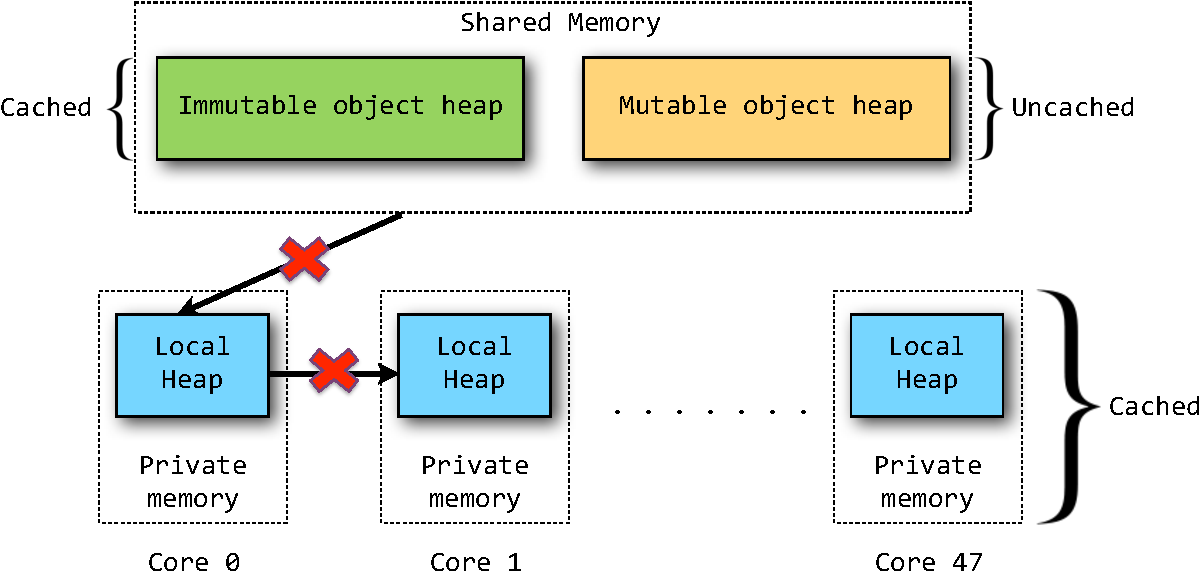
\includegraphics[width=0.8\textwidth]{Figures/SMC_Collector.pdf}
\caption{Heap design utilizing SCC's software-managed cache coherence capability.}
\label{fig:smc}
\end{figure}

\subsection{Heap Design}

The heap design for taking advantage of SMC is given in Figure~\ref{fig:smc}.
The design is similar to the local collector design (Section~\ref{sec:lc}) with
one key difference.  Instead of a single uncached shared heap, we split our
shared heap into cached and uncached partitions. We take advantage of the fact
that standard ML can statically distinguish between mutable and immutable
objects. Since immutable objects by definition will not change after
initialization, we enable caching on one of the shared heaps into which only
globalized immutable objects will be allocated. We call this heap a cached
shared heap (CSH). Since most objects in standard ML are immutable, we gain the
advantage of caching by placing these objects in CSH while not having to deal
with coherence issues. CSH is implemented using Software Managed Coherence
(SMC) for SCC~\cite{SMC}, and we mark CSH as a MPB type area such that any
cache line from CSH will be tagged as MPB type. The CSH cached data bypasses L2
and caching operates in a write-through mode.

Caching is disabled in the uncached shared heap (USH) into which globalized
mutable objects are allocated. By disabling caching, we circumvent the
coherence issues at the cost of performance. A local heap object being
globalized might contain both mutable and immutable objects in its transitive
object closure. Hence, globalization might involve allocating new objects in
both partitions of the shared heap. For the same reason, pointers are allowed
between the two partitions of the shared heap.

\subsection{Memory Consistency}

The key challenge now is to ensure that the updates to CSH are visible to all
the cores. Since CSH is cached, and SCC does not provide hardware cache
coherence, explicit cache invalidations and flushes must be implemented.
Moreover, any missed flushes or invalidations will lead to incoherent caches,
while frequent flushes or invalidations leads to poor performance. The key
observation is that the baseline local collector design has both read and write
barriers; our idea is to integrate the cache control primitives into the memory
barriers.

\begin{figure}[t]
\begin{lstlisting}
pointer readBarrier (pointer p) {
  if (!isPointer(p)) return p;
  if (getHeader(p) == FORWARDED) {
		/* Address in shared heap */
    p = *(pointer*)p;
		if (p > MAX_CSH_ADDR) {
			/* Address in cached shared heap, and has not
			 * been seen so far. Fetch the updates. */
			smcAcquire();
			MAX_CSH_ADDR = p;
		}
	}
  return p;
}
\end{lstlisting}
\caption{Read barrier with software-managed cache coherence capability.}
\label{code:read_barrier_smc}
\end{figure}

\begin{figure}[t]
\begin{lstlisting}
val writeBarrier (Ref r, Val v) {
  if (isObjptr(v) && isInSharedHeap(r) && isInLocalHeap(v)) {
			/* Move transitive object closure to shared
			 * heap, and install forwarding pointers */
			v = globalize (v);
			/* Publish the updates */
			smcRelease();
	}
	return v;
}
\end{lstlisting}
\caption{Write barrier with software-managed cache coherence capability.}
\label{code:write_barrier_smc}
\end{figure}


The CSH is always mapped to an address that is greater than the starting
address of the USH. Each core maintains the largest address seen in CSH in the
\cf{MAX\_CSH\_ADDR} variable. During an object read, if the address of the
object lies in the shared heap and is greater than \cf{MAX\_CSH\_ADDR}, we
invalidate any cache lines that might be associated with CSH by invoking
\texttt{smcAcquire()} (Line 9 in Figure~\ref{code:read_barrier_smc}). This
ensures that the values read are not stale. We update the \cf{MAX\_CSH\_ADDR}
if necessary. Since the objects in CSH are immutable, there is no need to
perform cache invalidation while reading an address that is less than
\cf{MAX\_CSH\_ADDR}. Additionally, after garbage collection,
\cf{MAX\_CSH\_ADDR} is set to point to the start of the CSH.

Similarly, whenever an object is globalized to the CSH, we must ensure that the
updates are visible to all of the cores. After an globalizing write, we invoke
\texttt{smcRelease()}, to flush any outstanding writes to the memory (Line 7 in
Figure~\ref{code:write_barrier_smc}).

\subsection{Mapping Channel Communication over Message-Passing Buffers}
\label{sec:comm_opt}

In this section, we describe how we map the \MM communication model on top of
the MPB. The main challenge here is the compatibility between the \MM
communication model and the capabilities of MPB. In \MM, threads communicate
over first-class channels, which support many-to-many communication pattern.
Hence, a receiver does not know the identity of the sender and vice versa.
Moreover, if a receiver is not available, the sender thread blocks; it is
descheduled, and some other thread from the scheduler queue continues execution
on that core. Moreover, the values sent over the channels in \MM can be
mutable. The channel itself is simply a data structure implemented over shared
memory. However, the communication on the SCC over libraries such as RCCE and
RCKMPI is optimized for SPMD programming model, where the sender and the
receiver know each other's identities, and are expected to arrive at the
communication point at the same time. Hence, considering the fact that MPB
memory is on 8KB, both RCCE and RCKMPI use busy waiting strategy for inter-core
communication. Thus, careful design is needed to map \MM communication
abstraction over the MPB.

Our channel mapping implementation exploits both the cached shared heap and MPB
for efficient inter-core message passing. We take advantage of our heap layout
and the availability of static type information to take advantage of the fast,
on-die MPB memory. We consider the following five cases:

\begin{enumerate}
\item Channel is located in the local heap
\item Channel is located in the shared heap, and the message being sent is an
unboxed value
\item Channel is located in the shared heap, the message is in the local heap,
and at least one of the objects in the transitive closure of the message being
sent is mutable
\item Channel is located in the shared heap, the message is in the local heap,
and all objects in the transitive closure of the message being sent are
immutable
\item Channel and the message are located in the shared heap
\end{enumerate}

For case 1, we observe that only channels that are located in the shared heap
can be used for inter-core communication. Our heap invariants prevent pointers
from one local heap to another. Thus, if a channel is located in the local
heap, then no thread on the other cores have a reference to this channel. Thus,
communication under case 1 only involves a value or a pointer exchange between
the communicating lightweight threads.

MultiMLton supports unboxed types that represent raw values. Hence, under case
2, we add a reference to the thread along with the value being sent to the
channel. In addition, we add a reference to the blocked thread to the
remembered list so that the local garbage collection can trace it.

\begin{figure}[t]
\centering
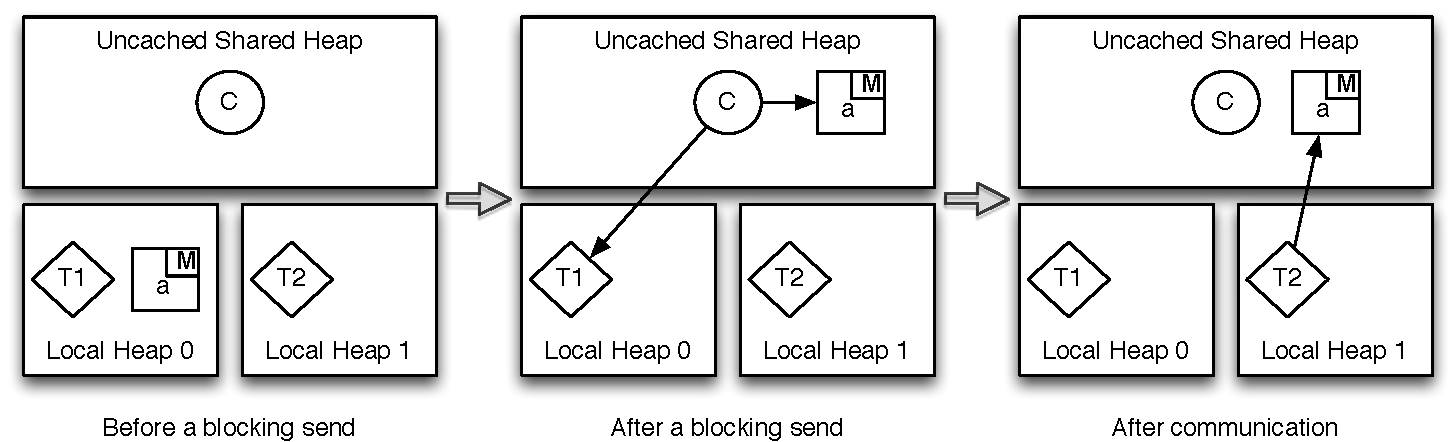
\includegraphics[width=1\textwidth]{Figures/Comm_Case_3}
\caption{Steps involved in sending an mutable object \cf{a} by thread \cf{T1}
on a shared heap channel \cf{C}, which is eventually received by thread
\cf{T2}.}
\label{fig:comm_mutable}
\end{figure}

If the message being sent has a mutable object in the transitive closure, we
must make this object visible to both the sender and the receiver core.
Figure~\ref{fig:comm_mutable} shows the case where a thread \cf{T1} sends a
mutable object \cf{a} on a shared heap channel \cf{C}. In this case, we eagerly
globalize \cf{a} before \cf{T1} blocks. Since the message is already in the
shared heap, when the receiver thread \cf{T2} eventually arrives, it just picks
up a pointer to the message in the shared heap.

\begin{figure}[t]
\centering
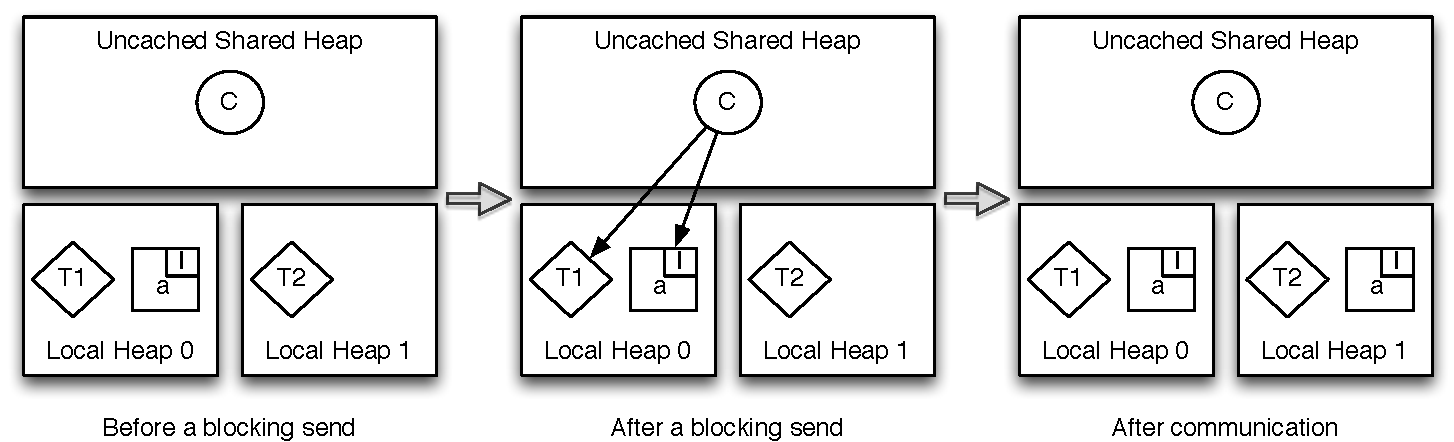
\includegraphics[width=1\textwidth]{Figures/Comm_Case_4}
\caption{Steps involved in sending an immutable object \cf{a} by thread \cf{T1}
on a shared heap channel \cf{C}, which is eventually received by thread
\cf{T2}.}
\label{fig:comm_immutable}
\end{figure}

Figure~\ref{fig:comm_immutable} shows the case where a thread \cf{T1} sends an
immutable object \cf{a} on a shared channel \cf{C}. Here, we simply add to the
channel \cf{C}, a reference to the message \cf{a} in the local heap, along with
the reference to the thread \cf{T1}. In addition, a reference to the object
\cf{a} is added to the remembered list, so that a local garbage collection will
be able to identify \cf{a} as being alive.

Afterward, when the receiver thread \cf{T2} arrives and finds the message not to
be in the shared heap, it sends an inter-core interrupt to the core on which the
message is located (core 0, in this case). After this message transfer is
initiated over the MPB using RCCE to transfer the object \cf{a} from core 0 to
core 1. Since Standard ML immutable objects do not have identity, making a copy
of the immutable object is safe under MultiMLton.

If the channel and the message are located in the shared heap, communication
only involves a value or a pointer exchange. This case is similar to case 1.

\section{Evaluation}
\label{sec:gc_bench}

The core, mesh controller, and memory on the SCC can be configured to run at
different frequencies. For our experiments we chose 533 MHz, 800 MHz, and 800
MHz for core, mesh, and memory respectively. In our results, wherever
appropriate, we present the 95\% confidence intervals, obtained using Student's
t-distribution.

For our experimental evaluation, we picked 8 benchmarks from the MLton
benchmark suite. The benchmarks were derived from sequential standard ML
implementation and were parallelized using ACML~\cite{Ziarek11}. The benchmarks
are:

\begin{itemize}
\item {\bf AllPairs}: an implementation of Floyd-Warshall algorithm for
computing all pairs shortest path.
\item {\bf BarnesHut}: an n-body simulation using Barnes-Hut algorithm.
\item {\bf CountGraphs}: computes all symmetries (automorphisms) within a set
of graphs.
\item {\bf GameOfLife}: Conway's Game of Life simulator
\item {\bf Kclustering}: a k-means clustering algorithm, where each stage is
spawned as a server.
\item {\bf Mandelbrot}: a Mandelbrot set generator.
\item {\bf Nucleic}: Pseudoknot~\cite{Pseudoknot} benchmark applied on multiple
inputs.
\item {\bf Raytrace}: a ray-tracing algorithm to render a scene.
\end{itemize}

\begin{table}[t]
\begin{center}
\caption{Benchmark characteristics. \%Sh represents the average fraction of
bytes allocated in the shared heap.}
\label{tab:bench_char}
\begin{tabular} {|l|r|r|r|r|}
\hline
\multirow{2}{*}{{\bf Benchmark}} & {\bf Allocation Rate} 	& \multicolumn{2}{|c|}{{\bf Allocation}} & \multirow{2}{*}{\bf \# Threads} \\
\cline{3-4}
																 & \multicolumn{1}{|c|}{{\bf (MB/s)}}						& {\bf Total (GB)} & {\bf \% Sh}	&	\\
\hline
{AllPairs} 		& 53 	\ci{2.3} & 16 \ci{0.23} 	& 11 	\ci{0.09} & 512 \\
{BarnesHut} 	& 70 	\ci{2.3} & 20 \ci{0.25} 	& 2		\ci{0.02} & 1024 \\
{CountGraphs} & 144 \ci{3.8} & 24 \ci{0.32} 	& 1		\ci{0.01} & 256 \\
{GameOfLife} 	& 127 \ci{5.0} & 21 \ci{0.47} 	& 13	\ci{0.17} & 1024 \\
{KClustering} & 108 \ci{2.9} & 32	\ci{0.31} 	& 3		\ci{0.05} & 1024 \\
{Mandelbrot} 	& 43 	\ci{1.7} & 2	\ci{0.02} 	& 8		\ci{0.03} & 512 \\
{Nucleic} 		& 87 	\ci{3.4} & 14	\ci{0.17} 	& 1		\ci{0.00} & 384 \\
{Raytrace} 		& 54 	\ci{2.6} & 12	\ci{0.14} 	& 4		\ci{0.03} & 256 \\
\hline
\end{tabular}
\end{center}
\end{table}

The benchmark characteristics is given in Figure~\ref{tab:bench_char}. The
numbers were obtained using local collector (\lc) with programs running on 48
cores, and the average of the results is reported. The benchmarks were designed
such that the input size and the number of threads are tunable. Out of the
total bytes allocated during the program execution, on average 5.4\% is
allocated in the shared heap. Thus, most of the objects allocated are collected
locally, without the need for stalling all of the mutators. The allocation rate
on the SCC is typically much lower than comparable general purpose commercial
offerings. On the SCC, not only is the processor slow (533MHz) but also the
serial memory bandwidth for our experimental setup is only around 70 MB/s.

\subsection{Performance}

\begin{figure}[t]
  \centering
  \subfigure[Speedup]{\label{fig:speedup}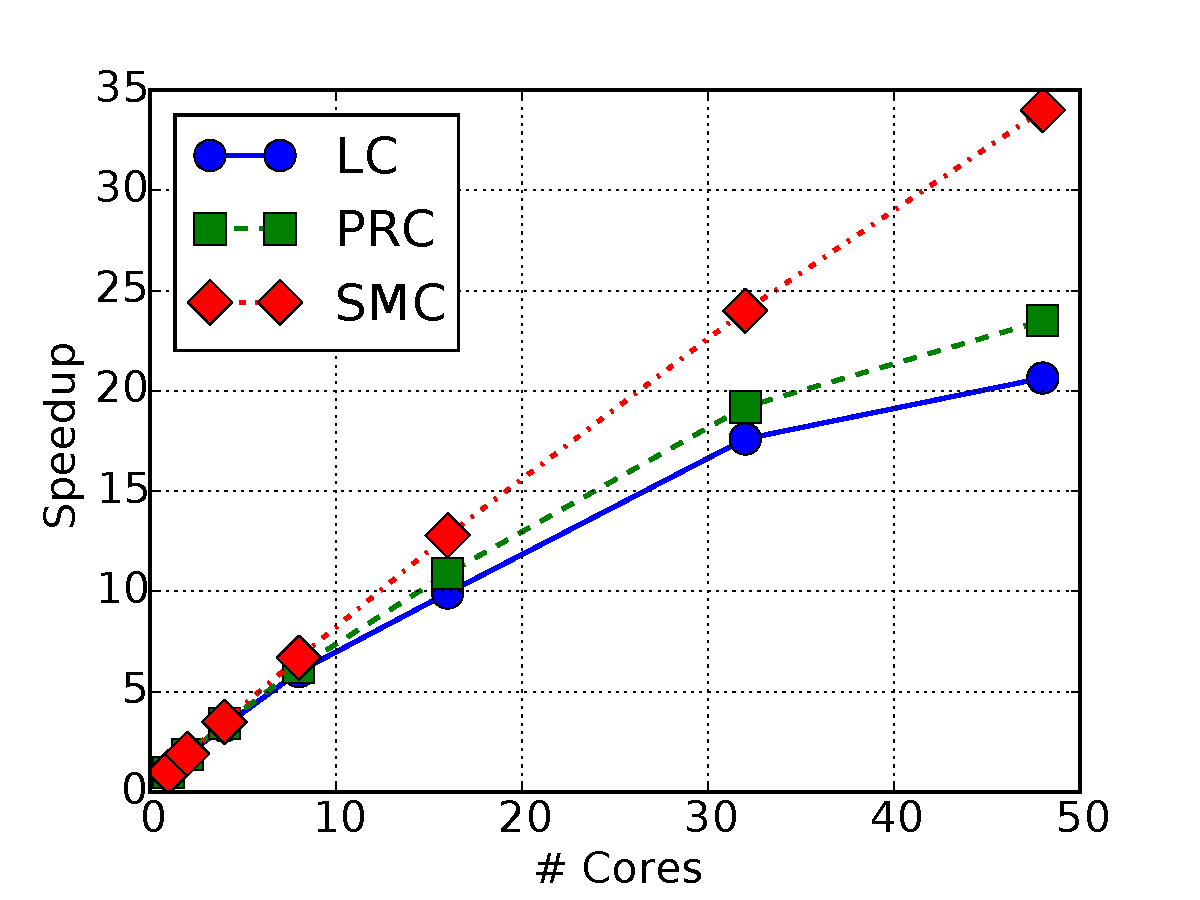
\includegraphics[width=0.45\textwidth]{Graphs/speedup_scc_heap}}
  \subfigure[Total time (48 cores)]{\label{fig:time_SCC}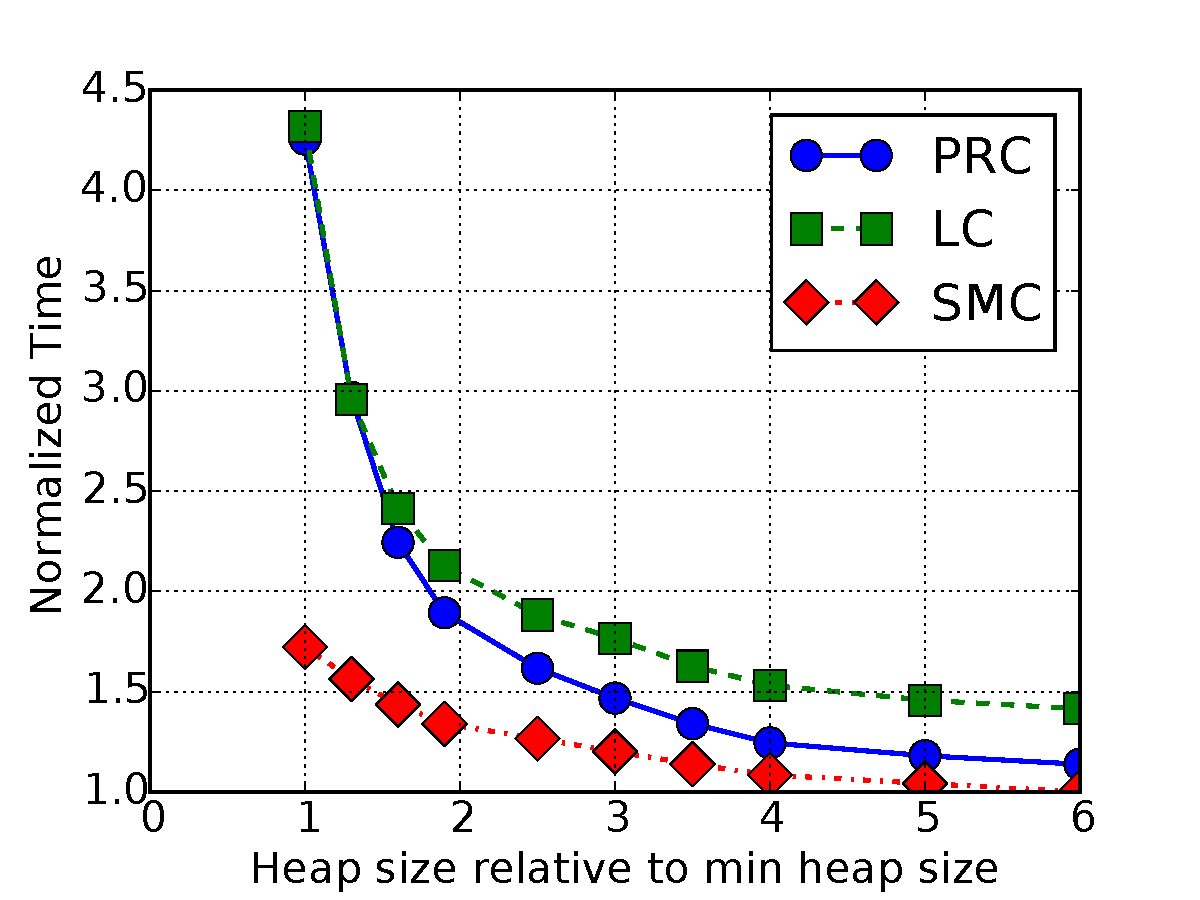
\includegraphics[width=0.45\textwidth]{Graphs/time_scc}}
  \subfigure[Mutator time (48 cores)]{\label{fig:mutator_time_SCC}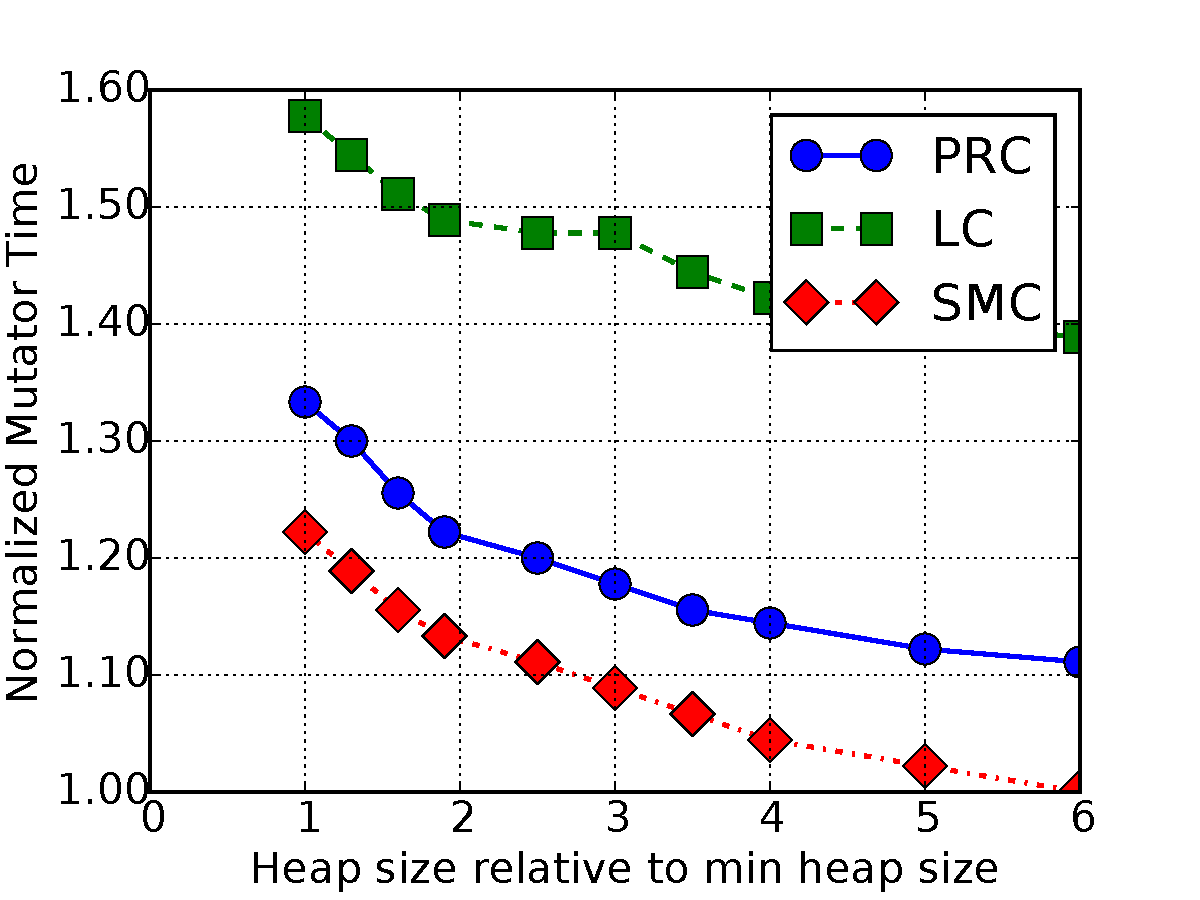
\includegraphics[width=0.45\textwidth]{Graphs/mutator_time_scc}}
  \subfigure[GC time (48 cores)]{\label{fig:gc_time_SCC}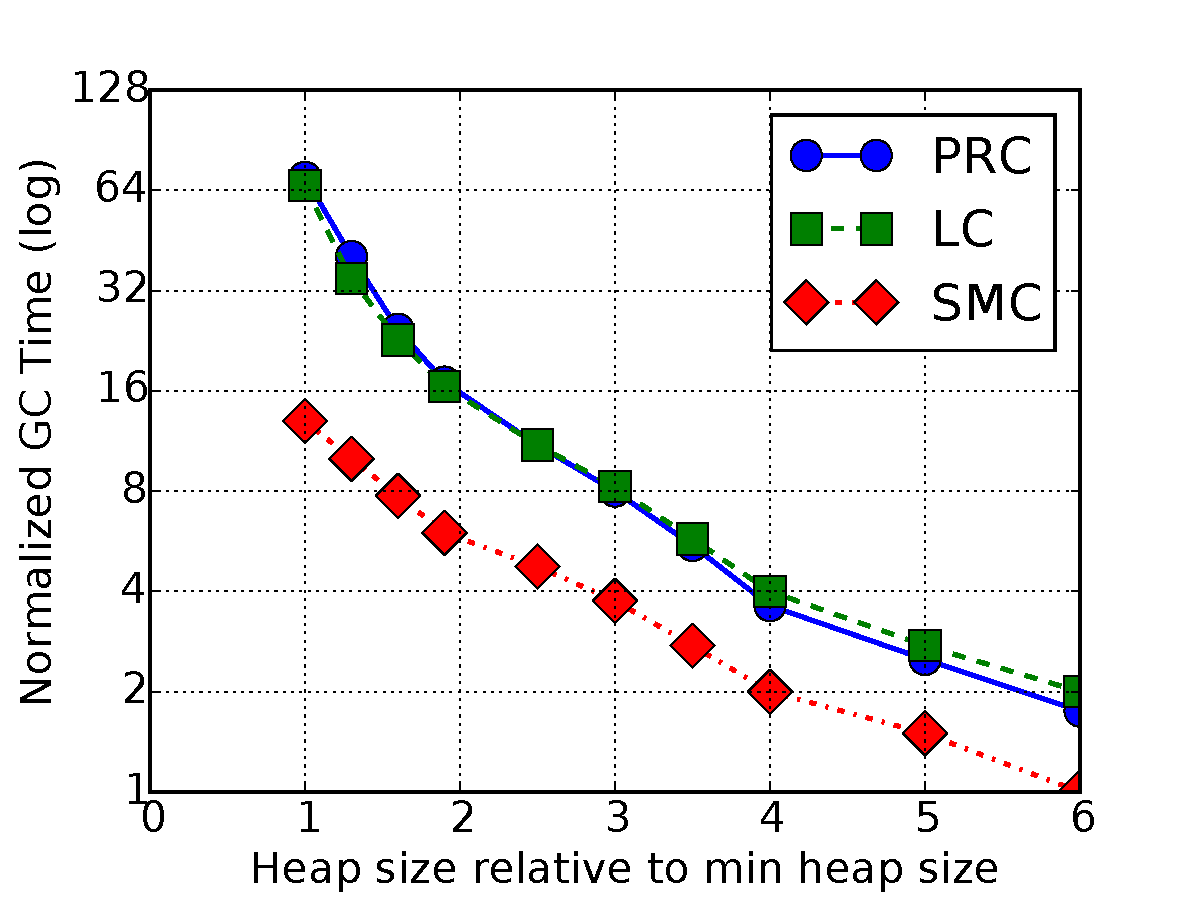
\includegraphics[width=0.45\textwidth]{Graphs/gc_time_scc}}
	\caption{Performance comparison of local collector with read barriers (\lc),
	procrastinating collector without read barriers (\prc), and collector
	utilizing software-managed cache coherence (SMC) : Geometric mean for 8
	benchmarks.}
  \label{fig:time}
\end{figure}

Figure~\ref{fig:time} presents the speedup results and illustrates space-time
trade-offs critical for any garbage collector evaluation. Among the three
variants, SMC performs the best (Figure~\ref{fig:speedup}) due to the fact that
most of the accesses under SMC is cached, unlike \lc and \prc. We also see that
the performance of \lc and \prc start to flatten out due to the contention on the
uncached shared memory as we increase the number of cores. Thus, with
increasing number of cores, the uncached shared memory becomes the bottleneck.

As we decrease the overall heap size, we see that the programs take longer to
run, due to the more frequent GCs (Figure~\ref{fig:time_SCC}). The reduction in
heap size, by definition, does not adversely affect the mutator time when
compared with the GC time. At 3$\times$ the minimum heap size under which the
programs would run, \prc is 17\% faster than \lc, and SMC is 18\% faster than
\prc. Overall, SMC is 32\% faster than \lc.

The mutator time (Figure~\ref{fig:mutator_time_SCC}) of \lc is consistently
higher than \prc due to the elimination of read barrier overheads under \prc.
Although SMC does have read barrier overheads, caching much of the shared
memory accesses keeps the mutator time low. We instrumented our read and write
barriers to classify the memory accesses. On average, across all of the
benchmarks, 89\% of the read or write requests were to the local heap, which is
private and is cached both in L1 and L2. This is common to all three versions
of the local collector. Thus, SMC derives mutator gains by caching much of the
11\% of the GC requests.

Out of the shared heap memory requests, on average, 93\% of all requests were
to the cached shared heap. However, it should be noted that cached shared heap
data bypass L2, and are only cached in the comparatively smaller L1 cache.
Hence, the benefit of caching shared heap data, as far as the mutator is
concerned, may not be dramatic if the cached shared heap reads are far and few
between. In any case, with SMC, less than 1\% of mutator accesses were to the
uncached memory. Thus, SMC is able to potentially cache more than 99\% of
memory accesses.

There is very little difference between the GC times
(Figure~\ref{fig:gc_time_SCC}) between \lc and \prc. This is because both the
variants are similar in terms of the actual GC work. However, SMC's GC time
tends to be lower since part of the expensive shared heap collection itself is
cached. Thus, software-managed cache coherence not only benefits the mutator
but also the garbage collector.

\subsection{Evaluating Procrastinating Collector}

In this section, we will focus on the procrastinating collector (\prc) design,
and analyze the impact of different optimizations.

\subsubsection{Impact of Cleanliness}
\label{sec:impact_cleanliness}

Cleanliness information allows the runtime system to avoid preempting threads
on a write barrier when the source of an globalizing write is clean. In order to
study the impact of cleanliness, we removed the reference counting code and
cleanliness check from the write barrier; thus, every globalizing write results
in a thread preemption and stall. The results presented here were taken with
programs running on 48-cores.

\begin{table}[t]
\begin{center}
\caption{Average number of preemptions on write barrier.}
\label{tab:preempt}
\begin{tabular} {|l|r|r|r|}
\hline
{\bf Benchmark} & {\bf \prc} & {\bf \prc MU-} & {\bf \prc CL-} \\
\hline
AllPairs 		& 604 \ci{42}		&	616 \ci{43}			&	28573 \ci{1429} \\
BarnesHut 	& 8376 \ci{503}	&	82284 \ci{3291}	& 23504887 \ci{1175244} \\
CountGraphs & 45 \ci{2}			&	64 \ci{2}				& 17061 \ci{1194} \\
GameOfLife 	& 11973 \ci{359} &	238462 \ci{16692}	& 1936250 \ci{58088} \\
KClustering & 7227 \ci{217}	& 15394 \ci{616}	& 8107173 \ci{405359} \\
Mandelbrot 	& 44 \ci{2}			& 84 \ci{5}				& 5863 \ci{235} \\
Nucleic 		& 58 \ci{3}			& 104594 \ci{4184}	&	209840 \ci{14689} \\
Raytrace 		& 881 \ci{35}		& 973 \ci{39}			& 13464 \ci{404} \\
\hline
\end{tabular}
\end{center}
\end{table}

Table~\ref{tab:preempt} shows the number of preemptions on write barrier for
different configurations. \prc represents the variant with all of the features
enabled; \prc MU- shows a cleanliness optimization that does not take an
object's mutability into consideration in determining cleanliness (using only
recorded reference counts instead), and \prc CL- represents preemptions incurred
when the collector does not use any cleanliness information at all. Without
cleanliness, on average, the programs perform substantially more preemptions
when encountering a write barrier.

Recall that if all of the threads belonging to a core get preempted on a write
barrier, a local major GC is \emph{forced}, which lifts all of the sources of
globalizing writes, fixes the references to forwarding pointers and unblocks the
stalled threads. Hence, an increase in the number of preemptions leads to an
increase in the number of local collections.

\begin{table}[t]
\begin{center}
\caption{Average percentage of forced GCs out of the total number of local
major GCs.}
\label{tab:forcedGCs}
\begin{tabular} {|l|r|r|r|}
\hline
{\bf Benchmark} & {\bf \prc} & {\bf \prc MU-} & {\bf \prc CL-} \\
\hline
AllPairs & 0.08 \ci{0} & 0.08 \ci{0} & 38.55 \ci{2.31} \\
BarnesHut & 0.17 \ci{0.01} & 19.2 \ci{0.96} & 100 \ci{3} \\
CountGraphs & 0 \ci{0} & 0.03 \ci{0} & 0.18 \ci{0.01} \\
GameOfLife & 3.54 \ci{0.21} & 9.47 \ci{0.47} & 99.75 \ci{4.99} \\
KClustering & 0 \ci{0} & 0.02 \ci{0} & 21.64 \ci{1.08} \\
Mandelbrot & 1.43 \ci{0.1} & 2.86 \ci{0.11} & 86.22 \ci{6.04} \\
Nucleic & 0 \ci{0} & 9.37 \ci{0.28} & 19.3 \ci{0.58} \\
Raytrace & 1.72 \ci{0.1} & 1.72 \ci{0.07} & 24.86 \ci{0.99} \\
\hline
\end{tabular}
\end{center}
\end{table}

Table~\ref{tab:forcedGCs} shows the percentage of local major GCs that were
forced compared to the total number of local major GCs. \prc CL- shows the
percentage of forced GCs if cleanliness information is not used. On average,
49\% of local major collection performed is due to forced GCs if cleanliness
information is not used, whereas it is less than 1\% otherwise.  On benchmarks
like {\tt BarnesHut}, {\tt GameOfLife} and {\tt Mandelbrot}, where all of the
threads tend to operate on a shared global data structure, there are a large
number of globalizing writes. On such benchmarks almost all local GCs are forced
in the absence of cleanliness. This adversely affects the running time of
programs.

\begin{figure}[t]
  \centering
  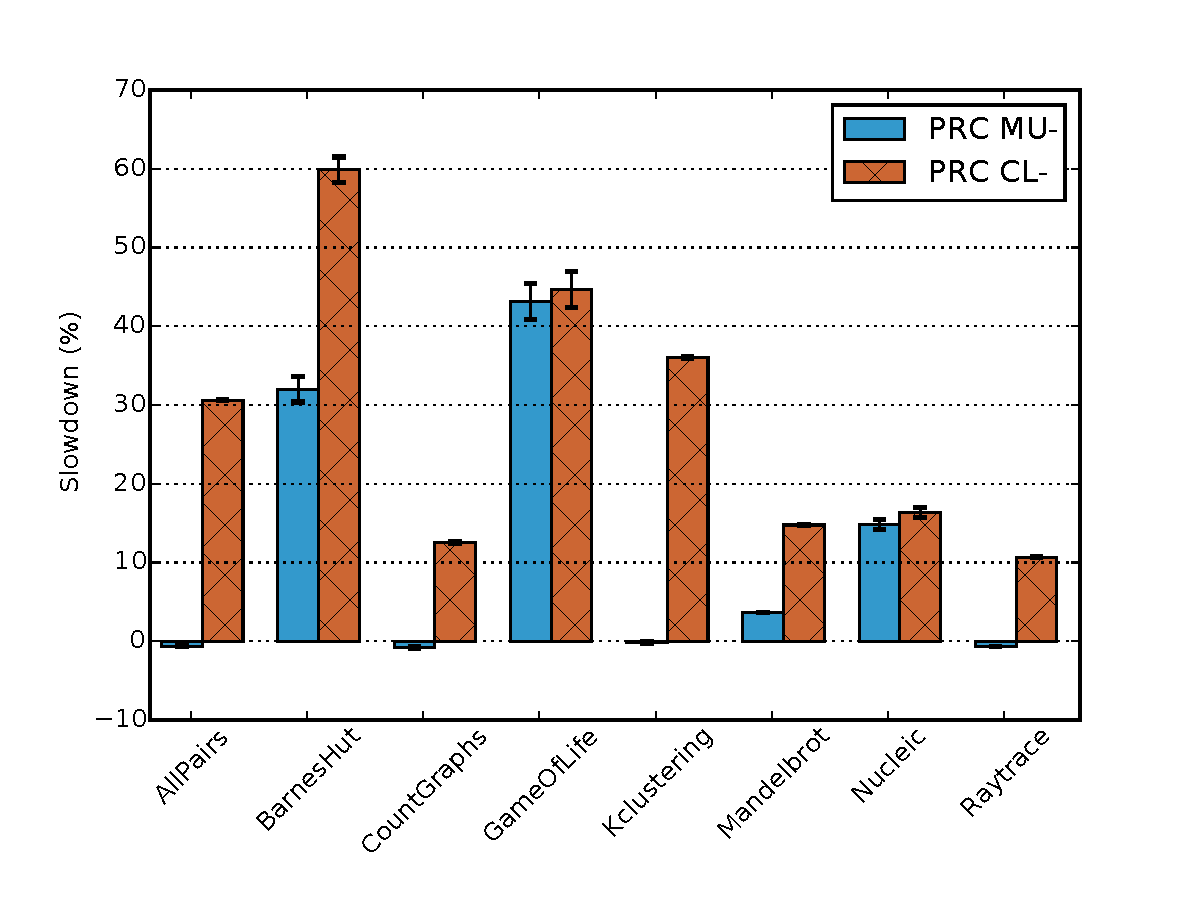
\includegraphics[width=0.8\textwidth]{Graphs/slowdown_cleanliness}
	\caption{Impact of utilizing object mutability information and cleanliness
	analysis on the performance of \prc.}
  \label{fig:slowdown-cleanliness}
\end{figure}

Figure~\ref{fig:slowdown-cleanliness} shows the running time of programs
without using cleanliness. On average, programs tend to run 28.2\% slower if
cleanliness information is ignored. The results show that cleanliness analysis
therefore plays a significant role in the \prc design.

\subsubsection{Impact of Immutability}

If the source of an globalizing write is immutable, we can make a copy of the
object in the shared heap and assign a reference to the new shared heap object
to the target. Hence, we can ignore the reference count of such objects. Not
all languages may have the ability to distinguish between mutable and immutable
objects in the compiler or in the runtime system. Hence, we study the impact of
our local collector design with mutability information in mind.  To do this, we
ignore the test for mutability in the cleanliness check
(Figure~\ref{code:cleanliness}) and modify the object lifting code in
Figure~\ref{code:lift} to treat all objects as mutable.

\prc MU- in Table~\ref{tab:preempt} and Table~\ref{tab:forcedGCs} show the
number of write barrier preemptions and the percentage of forced GCs,
respectively, if all objects were treated as mutable.  For some programs such
as {\tt AllPairs}, {\tt CountGraphs}, or {\tt Kclustering}, object mutability
does not play a significant factor.  For benchmarks where it does,
distinguishing between mutable and immutable objects helps avoid inducing
preemptions on a write barrier since a copy of the immutable object can be
created in the shared heap without the need to repair existing references to
the local heap copy.

Figure~\ref{fig:slowdown-cleanliness} shows the performance impact of taking
object mutability into account. While ignoring object mutability information,
{\tt BarnesHut}, {\tt GameOfLife} and {\tt Nucleic} are slower due to the
increased number of forced GCs. Interestingly, {\tt AllPairs}, {\tt
CountGraphs}, {\tt Kclu\allowbreak stering} and {\tt Raytrace} are marginally
faster if the mutability information is ignored. This is due to not having to
manipulate the \cf{imSet} (Line 15 in Figure~\ref{code:lift}), and walking
immutable objects after the objects are lifted (Line 22 in
Figure~\ref{code:lift}). On average, we see a 11.4\% performance loss if
mutability information is not utilized for cleanliness.

\subsubsection{Impact of Heap Session}
\label{sec:impact_session}

\begin{table}
\begin{center}
\caption{Impact of heap session: \% LM clean represents the fraction of
instances when a clean object closure has at least one object with
\cf{LOCAL\_MANY} references.}
\label{tab:session-impact}
\begin{tabular} {|l|r|r|r|}
\hline
{\bf Benchmark} & {\bf \% LM Clean} & {\bf Avg. Session Size (Bytes)} \\
\hline
AllPairs & 5.35 \ci{0.37} & 2966 \ci{119} \\
Barneshut & 13.27 \ci{0.53} & 1596 \ci{96} \\
Countgraphs & 8.86 \ci{0.53} & 3648 \ci{73} \\
GameOfLife & 23.9 \ci{1.2} & 1384 \ci{55} \\
Kclustering & 18.13 \ci{0.54} & 2248 \ci{135} \\
Mandelbrot & 4.64 \ci{0.09} & 8549 \ci{598} \\
Nucleic & 13.3 \ci{0.27} & 1226 \ci{37} \\
Raytrace & 8.28 \ci{0.41} & 1112 \ci{22} \\
\hline
\end{tabular}
\end{center}
\end{table}

In order to assess the effectiveness of using heap sessions, we measured the
percentage of instances where the source of an globalizing write is clean with at
least one of the objects in the closure has a \cf{LOCAL\_MANY} reference.
During such instances, we walk the current heap session to fix any references
to forwarded objects. Without using heap sessions, we would have preempted the
thread in the write barrier, reducing  available concurrency. The results are
presented in Table~\ref{tab:session-impact}.

The first column shows the percentage of instances when an object closure is
clean and has at least one object with \cf{LOCAL\_MANY} references. On average,
we see that 12\% of clean closures have at least one object with
\cf{LOCAL\_MANY} references. We also measured the average size of heap sessions
when the session is traced as a part of lifting an object closure to the shared
heap (Line 25 in Figure~\ref{code:lift}). The average size of a heap session
when it is traced is 2859 bytes, which is less than a page size. These results
show that utilizing heap sessions significantly contributes to objects being
tagged as clean, and heap sessions are small enough to not introduce
significant overheads during tracing.


\subsection{MPB Mapped Channels}

\begin{figure}[t]
\centering
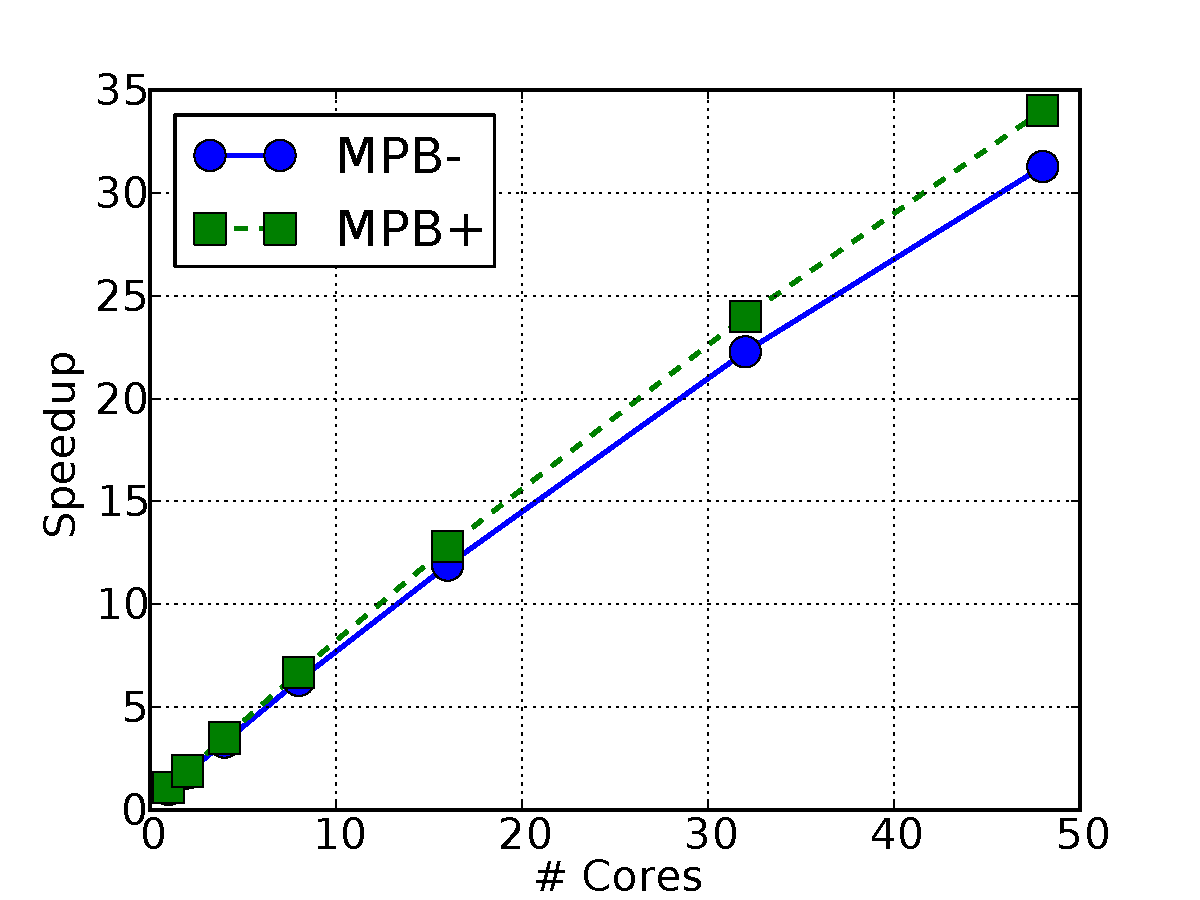
\includegraphics[width=0.5\textwidth]{Graphs/speedup_scc_chan}
\caption{Performance comparison of first-class channel communication over the
MPB \cf{(MBP+)} vs solely over the shared memory \cf{(MPB-)}: Geometric mean
over 8 benchmarks.}
\label{fig:speedup_scc_chan}
\end{figure}


In this section, we study the impact of MPB mapped channels. In order to
evaluate the benefit of mapping the first-class channel communication over the
message passing buffer memory, we implemented a version of our communication
library that does not use the message passing buffer memory. Recall that if the
channel is located in the shared heap, the message in the local heap, and the
message does not have a mutable object in its transitive closure, we perform
the transfer over the message passing buffer (Case 4 in
Section~\ref{sec:comm_opt}). Instead, we eagerly globalize the transitive
closure of the message and just share the pointer with the receiving thread
(similar to Case 3). We call this version MPB-, and the original version MPB+.

Figure~\ref{fig:speedup_scc_chan} shows the performance comparison of MPB+
versus MPB-. On 48-cores, MPB+ is only around 9\% faster than the MPB- version.
We can attribute several reasons for this marginal improvement. First, we
observed that, on average, around only 32\% of channel communications were
taking advantage of the MPB (Case 4) in the case of MPB+. The rest of the
channel communications were either local or were using the shared memory to
transfer the messages. Moreover, in the case of MPB-, immutable inter-core
messages are transferred over the CSH which is cached.

Second, the cost of inter-core interrupts is substantial, as was observed by
others~\cite{Peter11,Darko11}. We measured the time it takes between a core
issuing an inter-core interrupt to the time it sends or receives the first byte
is around 2000 core cycles. Since majority of the immutable messages exchanged
between cores are small, the overhead of setting up the message transfer
outweighs the benefit of using the MPB. However, utilizing the MPB prevents
immutable messages from being globalized, thus reducing the pressure on the
shared memory. As a result, the number of expensive shared heap collections are
reduced.

\section{Related Work}

Over the years, several local collector designs ~\cite{Steele75, Doligez93,
Steensgaard00, Anderson10} have been proposed for multi-threaded programs.
Recently, variations of local collector design have been adopted for
multi-threaded, functional language runtimes like GHC~\cite{Marlow11} and
Manticore~\cite{Auhagen11}. Doligez et al.~\cite{Doligez93} proposed a local
collector design for ML with threads where all mutable objects are allocated
directly on the shared heap, and immutable objects are allocated in the local
heap. Similar to our technique, whenever local objects are shared between
cores, a copy of the immutable object is made in the shared heap. Although this
design avoids the need for read and write barriers, allocating all mutable
objects, irrespective of their sharing characteristics can lead to poor
performance due to increased number of shared collections, and memory access
overhead due to NUMA effects and uncached shared memory as in the case of SCC.
It is for this reason we do not treat the shared memory as the oldest
generation for our local generation collector unlike other
designs~\cite{Doligez93, Marlow11}.

Several designs utilize static analysis to determine objects that might
potentially escape to other threads~\cite{Jones05, Steensgaard00}. Objects that
do not escape are allocated locally, while all others are allocated in the
shared heap. The usefulness of such techniques depends greatly on the precision
of the analysis, as objects that might potentially be shared are allocated on
the shared heap. This is undesirable for architectures like the SCC where
shared memory accesses are very expensive compared to local accesses. Compared
to these techniques, our design only exports objects that are definitely shared
between two or more cores. Our technique is also agnostic to the source
language, does not require static analysis, and hence can be implemented as a
lightweight runtime technique.

Anderson~\cite{Anderson10} describes a local collector design (TGC) that
triggers a local garbage collection on every globalizing write of a mutable
object, while immutable objects, that do not have any pointers, are copied to
the shared heap. This scheme is a limited form of our cleanliness analysis. In
our system, object cleanliness neither solely relies on mutability information,
nor is it restricted to objects without pointer fields. Moreover, TGC does not
exploit delaying globalizing writes to avoid local collections. However, the
paper proposes several interesting optimizations that are applicable to our
system. In order to avoid frequent mutator pauses on globalizing writes, TGC's
local collection runs concurrently with the mutator. Though running compaction
phase concurrently with the mutator would require read barriers, we can enable
concurrent marking to minimize pause times. TGC also proposes watermarking
scheme for minimizing stack scanning, which can be utilized in our system to
reduce the stack scanning overheads during context switches and globalizing
writes of clean objects.

Marlow et al.~\cite{Marlow11} propose globalizing only part of the transitive
closure to the shared heap, with the idea of minimizing the objects that are
globalized. The rest of the closure is exported essentially on demand during
the next access from another core. This design mandates the need for a read
barrier to test whether the object being accessed resides in the local heap of
another core. However, since the target language is Haskell, there is an
implicit read barrier on every load, to check whether the thunk has already
been evaluated to a value. Since our goal is to eliminate read barriers, we
choose to export the transitive closure on an globalizing write.

Software managed cached coherence (SMC)~\cite{SMC} for SCC provides a coherent,
shared virtual memory to the programmer. However, the distinction between
private and shared memory still exists and it is the responsibility of the
programmer to choose data placement. In our system, all data start out as being
private, and is only shared with the other cores if necessary. The sharing is
performed both through the shared memory as well as over the MPB, based on the
nature of message being shared. MESH framework~\cite{Prescher11} provides a
similar mechanism for flexible sharing policies on the SCC as a middle-ware
layer.

In the context of mapping first-class channels to MPBs, the work by Prell et
al.~\cite{Prell12} which presents an implementation of Go's concurrency
constructs on the SCC is most similar. However, unlike our channel
implementation, channels are implemented directly on the MPB. Since the size of
MPB is small, the number of channels that can be concurrently utilized are
limited. Moreover, their implementation diverges from Go language specification
in that the go-routines running on different cores run under different address
spaces. Hence, the result of transferring a mutable object over the channels is
undefined. Our channel communication utilizes both shared memory and the MPBs
for inter-core messaging. Barrelfish on the SCC~\cite{Peter11} uses MPBs to
transfer small messages and bulk transfer is achieved through shared memory.
However, Barrelfish differs from our system since it follows a shared-nothing
policy for inter-core interaction.

\section{Concluding Remarks}

The Intel SCC provides an architecture that combines aspects of distributed
systems (no cache coherence) with that of a shared memory machine, with support
for programmable cache coherence and fast inter-core messaging. In order to
effectively utilize this architecture, it is desirable to hide the complexity
behind the runtime system. To this end, the \MMSCC programming platform
provides a cache coherent shared memory abstraction for the ML programmer.
\MMSCC utilizes the mostly-functional and highly concurrent nature of the
programming model to implement a memory management scheme that is optimized for
the memory hierarchy found on the SCC. The results and experience building
\MMSCC illustrate that functional programming language technology can mitigate
the burden of developing software for highly scalable manycore systems.

\newcommand{\denote}[1]{\lbrack\!\lbrack#1\rbrack\!\rbrack}
\newcommand{\emeaning}[1]{{\cal D}\lbrack\!\lbrack#1\rbrack\!\rbrack}

\lstset{ %
language=ML, % choose the language of the code
basicstyle=\footnotesize\ttfamily,       % the size of the fonts that are used for the code
keywordstyle=\color{Bittersweet},
%numbers=left,                   % where to put the line-numbers
%numberstyle=\tiny,      % the size of the fonts that are used for the line-numbers
%stepnumber=1,                   % the step between two line-numbers. If it is 1 each line will be numbered
%numbersep=5pt,                  % how far the line-numbers are from the code
%backgroundcolor=\color{white},  % choose the background color. You must add \usepackage{color}
showspaces=false,               % show spaces adding particular underscores
showstringspaces=false,         % underline spaces within strings
showtabs=false,                 % show tabs within strings adding particular underscores
frame=single,                   % adds a frame around the code
tabsize=2,                      % sets default tabsize to 2 spaces
captionpos=b,                   % sets the caption-position to bottom
breaklines=true,                % sets automatic line breaking
breakatwhitespace=false,        % sets if automatic breaks should only happen at whitespace
commentstyle=\itshape\color{MidnightBlue},
%escapeinside={\%*}{*)},         % if you want to add a comment within your code
}

%Formatting Commands
%-------------------
\renewcommand{\R}[1]{\textrm{#1}}
\renewcommand{\k}[1]{\mathtt{#1}} % Code font in math mode.
%\newcommand{\code}[1]{\,{\tt #1}\,}
\newcommand{\tab}{\hspace*{1.5em}}
\newcommand{\conj}{~\wedge~}
\newcommand{\disj}{~\vee~}
\newcommand{\fixme}[1]{\fbox{\textsl{\bf #1}}}
\newcommand{\pairedup}{{\cal P}}
\newcommand{\sender}{{\cal S}}
\newcommand{\intrastate}{{\sf State}_{\sf intra}}
\newcommand{\intralabel}{{\sf Label}_{\sf intra}}
\newcommand{\SCFN}[1]{{\sc\footnotesize {#1}}}
\newcommand{\ready}{\R{\SCFN{Ready}}}
\newcommand{\done}{\R{\SCFN{Done}}}
\newcommand{\obs}{{\sf obs}}
\newcommand{\obsE}{{\sf ObsE}}
\newcommand{\restrict}[2]{[#1]_{#2}}
\newcommand{\filter}[2]{#1{\downarrow}_{#2}}
\newcommand{\isucc}[1]{~{\sf isucc}_{#1}~}
\newcommand{\synthesize}{\triangleright}
\newcommand{\One}{{\sf One}}
\newcommand{\All}{{\sf All}}
\newcommand{\rel}{\R{\SCFN{Rel}}}
\newcommand{\intraTraceSet}{\sf InTr^{\program}}
\newcommand{\cml}{\R{\SCFN{Cml}}}

%Attributes
%----------
\newcommand{\synchrony}{\sigma}
\newcommand{\fifo}{\phi}
\newcommand{\reliability}{\rho}
\newcommand{\ptop}{\pi}

%Classes
%-------
\newcommand{\SelectClass}{\mathbb{S}}
\newcommand{\ChannelClass}{\mathbb{C}}
\newcommand{\ChannelStateClass}{\mathbb{S}}
\newcommand{\ValueClass}{\mathbb{V}}
\newcommand{\NumberClass}{\mathbb{N}}
\newcommand{\ThreadClass}{\mathbb{T}}
\newcommand{\AttributeClass}{\mathbb{K}}
\newcommand{\ActionClass}[1]{\mathbb{A}_{#1}}

%Relations
%---------
\newcommand{\po}{\rightarrow_{po}} %Program order
\newcommand{\co}{\rightarrow_{co}} %Communication order
\newcommand{\mo}{\rightarrow_{mo}} %Match order
\newcommand{\bico}{\leftrightarrow_{co}} %Communication order
\newcommand{\cd}{\rightarrow_{cd}} %Channel dependence
\newcommand{\sw}{\rightarrow_{sw}} %Synchronizes-with
\newcommand{\td}{\rightarrow_{td}} %Thread dependence
\newcommand{\tr}{\rightarrow_{tr}} %Trace
\newcommand{\hb}{\rightarrow_{hb}} %Happens-before relation
\newcommand{\nhb}{\nrightarrow_{hb}} %Happens-before neg
\newcommand{\nbihb}{\nleftrightarrow_{hb}} %Bi-happens-before neg
\makeatletter
\def\twoheadrightarrowfill@{\arrowfill@\relbar\relbar\twoheadrightarrow}
\newcommand{\intratrans}[2][] {\ext@arrow035{13}\twoheadrightarrowfill@{#1}{#2}}
\newcommand{\intertrans}[1]{\xrightarrow{#1}}
\makeatother

%Execution
%---------
%\newcommand{\CommMatch}{{\sf M}}
\newcommand{\ActionSet}{{\sf A}}
\newcommand{\ChannelStates}{{\sf C}}
\newcommand{\program}{{\sf P}}
\newcommand{\Exec}{\langle \program, \allowbreak \ActionSet, \allowbreak \po, \allowbreak \co \rangle}
\newcommand{\E}{{\sf E}}

%% op semantics

\newcommand{\DepGraph}{\Gamma}
\newcommand{\ActionSoup}{\Delta}
\newcommand{\CommitSet}{\Omega}


\newcommand{\HLREL}[1]{\R{\textsf{HL-REL}}(#1)}
\newcommand{\LLREL}[1]{\R{\textsf{LL-REL}}(#1)}
\newcommand{\CML}[1]{\R{\textsf{CML}}(#1)}
\newcommand{\EP}{{\sf E'}}
\newcommand{\toto}{\rightarrow_{to}} 								%Total order
\newcommand{\totoP}{\rightarrow_{to'}} 							%Total order prime
\newcommand{\totoPP}{\rightarrow_{to''}} 						%Total order double prime
\newcommand{\so}{\rightarrow_{so}} 									%Spawn Order
\newcommand{\ko}{\rightarrow_{ko}} 									%C(K)ommit order

\newcommand{\rulelabel}[1]{\textrm{\sc {[#1]}}}
\newcommand{\RULE}[2]{\frac{\begin{array}{c}#1\end{array}}
                           {\begin{array}{c}#2\end{array}}}

\newcommand{\OExec}[3]{\langle #1, #2 \rangle_{#3}}
\newcommand{\ExecP}{\langle {\sf P}, \ActionSet,\po,\co \rangle}
\newcommand{\PrgState}[2]{\langle (t,E[#1]) \;\|\; \threadsoup,#2 \rangle}

\newcommand{\trace}{\mathit{tr}}
\newcommand{\commit}[2]{\epsilon_{(#1,#2)}}

\newcommand{\name}{\ftextrecipe$^{\mbox{\tiny\sc CML}}$}


\newcommand{\wf}[1]{{\sf WF}(#1)}
\newcommand{\transOpAx}[2]{\opax(#1,#2)}

\newcommand{\filtera}[2]{#1{\downarrow}_{#2}}

\newcommand{\thread}{\mathit{T}}
\newcommand{\threadid}{\textsf{t}}
\newcommand{\spawn}{\textsf{spawn}}
\newcommand{\unit}{\textsf{unit}}
\newcommand{\threadsoup}{\overline{\mathit{T}}}
\newcommand{\threadsoupp}{\overline{\mathit{T'}}}
\newcommand{\eval}[1]{\mathit{E}[#1]}
\newcommand{\evaln}{\mathit{E}}
\newcommand{\chan}{\textsf{ch}}
\newcommand{\send}{\textsf{send}}
\newcommand{\recv}{\textsf{recv}}
\newcommand{\join}{\textsf{join}}
\newcommand{\con}{\textsf{Con}}
\newcommand{\prev}{\textsf{Prev}}
\newcommand{\fresh}{\textsf{fresh}}
\newcommand{\print}{\textsf{print}}
\newcommand{\tupletwo}[2]{(#1,#2)}
\newcommand{\ALT}{~\mid~}
\newcommand{\ruleref}[1]{{\sc\small [#1]}}
\renewcommand{\bar}{\overline}

\newcommand{\opIntraState}[1]{E[#1]}
\newcommand{\readyOp}[1]{\R{\SCFN{Ready}}_{op}(#1)}
\newcommand{\doneOp}{\R{\SCFN{Done}}_{op}}
\newcommand{\localstate}{L}
\newcommand{\ProgramState}{\R{\SCFN{ProgState}}}
%\newcommand{\opax}{{\cal T}^{\stackrel[{\sc Op}]{{\sc Ax}}{\uparrow}}}
\newcommand{\opax}{{\cal T}^{\mbox{\tiny\sc op}}_{\mbox{\tiny\sc ax}}}
\newcommand{\opaxGen}{{\cal G}^{\mbox{\tiny\sc op}}_{\mbox{\tiny\sc ax}}}
\newcommand{\axcml}{\R{\SCFN{Ax$_2$Cml}}}




\chapter{\rxcml: A Prescription for Safely Relaxing Synchrony}

Concurrent ML~\cite{Reppy07} (CML) provides an expressive concurrency mechanism
through its use of first-class composable synchronous events.  When
synchronized, events allow threads to communicate data via message-passing over
first-class channels.  Synchronous communication simplifies program reasoning
because every communication action is also a synchronization point; thus, the
continuation of a message-send is guaranteed that the data being sent has been
successfully transmitted to a receiver.

The programming model of CML, however, assumes strong consistency; while the
channel itself is first-class and supports many-to-many communication pattern,
the communication has \emph{exactly-once} requirement. If a receiver consumes a
sent value, then no other sender can consume the same value. Thus, synchronous
communication needs coordination between the communicating parties for
enforcing the exactly-once requirement. Hence, while first-class channel based
synchornous communication provides a good abstraction, its correctness and
performance implication in a high latency, weakly consistent setting prevets
its utility in a weakly consistent loosely coupled environment.

While asynchronous extensions such as \acml~\cite{Ziarek11} can be used to gain
performance, they sacrifice the simplicity provided by synchronous
communication in favor of a more complex and sophisticated set of primitives.
Moreover, \acml also requires the \emph{exactly-once} requirement. Hence, even
though \acml solves the problem of synchrony at the cost of increased
complexity, it does not solve the problem of coherence.

One way to enhance performance without requiring new additions to the core set
of event combinators CML supports, is to give the underlying runtime the
freedom to allow a sender to communicate data asynchronously. In this way, the
cost of synchronous communication can be masked by allowing the sender's
continuation to begin execution even if a matching receiver is not yet
available. Because asynchrony is introduced only by the runtime, applications
do not have to be restructured to explicitly account for new behaviors
introduced by this additional concurrency.  Thus, we wish to have the runtime
enforce the equivalence: $\denote{\cf{send}(c,v)}k \equiv
\denote{\cf{asend}(c,v)}k$ where $k$ is a continuation, $\cf{send}$ is CML's
synchronous send operation that communicates value $v$ on channel $c$, and
$\cf{asend}$ is an asynchronous variant that buffers $v$ on $c$ and does not
synchronize on a matching receiver.

To illustrate, consider the following simple program:

\begin{center}
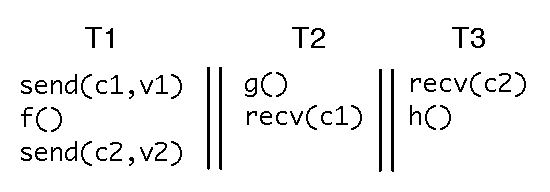
\includegraphics{Figures/IntroCode1}
\end{center}

\noindent Thread T1 performs a synchronous send on channel \cf{c1} that is
received by thread T2, after it computes \cf{g()}.  After the communication is
performed, T1 evaluates \cf{f()}, and then sends \cf{v2} on channel \cf{c2},
which is received by thread T3.  Upon receipt, T3 evaluates \cf{h()}. Assuming
\cf{f},\cf{g}, and \cf{h} perform no communication action of their own, the
synchronous communication on \cf{c1} by T1 could have been safely converted
into an asynchronous action in which \cf{v1} is buffered, and read by T2 later
upon evaluation of \cf{g()}.  The observable behavior of the program in both
cases (i.e., treating the initial send synchronously or asynchronously) would
be the same.

\begin{figure}[b]
\centering
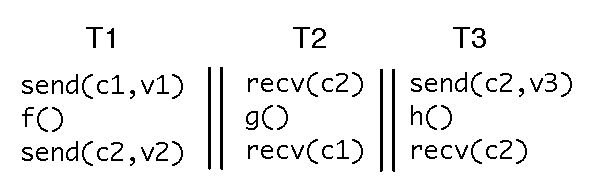
\includegraphics{Figures/IntroCode2}
\caption{Performing the first \cf{send} in T1 asynchronously is not meaning
preserving with respect to synchronous evaluation.}
\label{fig:intro2}
\end{figure}

Unfortunately, na\"{i}vely replacing synchronous communication with an
asynchronous one is not usually meaning-preserving as the example in
Figure~\ref{fig:intro2} illustrates. Under a synchronous evaluation protocol,
T2 would necessarily communicate first with T3, receiving \cf{v3} on channel
\cf{c2}.  It is then able to receive \cf{v1} from T1; finally, T1 can
communicate \cf{v2} to T3.  If the \cf{send(c1,v1)} operation by T1 were
replaced by \cf{asend(c1,v1)}, the first receive on T2 has, in addition to the
first send on T3, a \emph{new potential matching opportunity} -- the send of
\cf{v2} on channel \cf{c2}. If the receive by T2 matches with the send of
\cf{v2} on channel \cf{c2}, it is impossible to satisfy the send on T3. Thus,
this asynchronous execution exhibits a new behavior not possible using just
synchronous operators.

The distinction between these two executions can be explained in terms of a
dependence graph that captures both intra- and inter-thread data- and
control-flow.  We can depict the executions by explicitly drawing these
dependencies as shown below:

\begin{center}
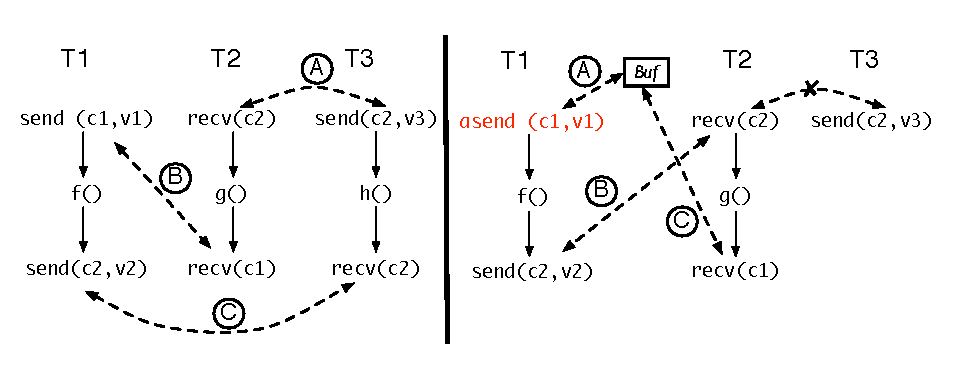
\includegraphics{Figures/IntroDepGraph}
\end{center}

\noindent The dashed edges reflect communication and synchronization
dependencies among threads, while solid edges capture thread-local
control-flow. A bi-directional edge connects a sender with either a
receiver, in the case of a synchronous send, or a buffer, in the case where
it is asynchronous.  In both instances, there is a synchronization
dependence between endpoints, and a data dependence from the sender to
either the matching receiver or buffer.  The left-hand side of the figure
shows a possible execution in which all operations are synchronous; the
right considers an execution in which the initial send by T1 is
asynchronous.  The labels on the edges reflect the order in which
communication actions are executed.

\newcommand*\mycirc[1]{%
  \begin{tikzpicture}[baseline=(char.base)]
    \node[shape=circle,draw,inner sep=.3pt] (char) {#1};
  \end{tikzpicture}}

The synchronous execution on the left reflects the description given earlier.
The asynchronous execution on the right depicts the send on thread T1 buffering
its data (\mycirc{A}), thus allowing the synchronous communication between T1
and T2 (\mycirc{B}); this action prohibits communication between T2 and T3.  T2
subsequently receives \cf{v1} from the buffer associated with channel \cf{c1}
(\mycirc{C}).  This behavior could not be realized by any synchronous
execution: \mycirc{B} could never have been performed if the send operation on
channel \cf{c1} was not asynchronous.

The formalization of \emph{well-formed executions}, those that are the result
of asynchronous evaluation of CML send operations, but which nonetheless are
observably equivalent to a synchronous execution, and the means by which
erroneous executions, such as the right-hand execution above, can be detected
and repaired, form the focus of this chapter. Specifically, we make the
following contributions:

\begin{itemize}

\item We present the rationale for a \emph{relaxed execution model} for CML
that specifies the conditions under which a synchronous operation can be safely
executed asynchronously.  Our model allows applications to program with the
simplicity and composability of CML synchronous events, but reap the
performance benefits of implementing communication asynchronously.

\item We develop an axiomatic formulation of the model that can be used to
reason about correctness in terms of causal dependencies captured by a
\emph{happens-before} relation.  We relate this definition to an operational
semantics that specifies relaxed execution behavior for communicating actions,
and relate the set of traces admitted by the operational semantics to the safe
executions defined by the axiomatic formulation.

\item A distributed implementation, \rxcml, that treats asynchronous
communication as a form of \emph{speculation} is described. A mis-speculation,
namely the execution that could not have been realized using only synchronous
communication, is detected using a runtime instantiation of our axiomatic
formulation. An un-coordinated, distributed checkpointing mechanism is utilized
to rollback and re-execute the offending execution synchronously, which is
known to be safe.

\item Several case studies on a realistic cloud deployment demonstrate the
utility of the model in improving the performance of CML programs in
distributed environments without requiring \emph{any} restructuring of
application logic to deal with asynchrony.

\end{itemize}

\section{Motivation}

To motivate the utility of safe relaxation of synchronous behavior, consider
the problem of building a distributed chat application. The application
consists of a number of participants, each of whom can broadcast a message to
every other member in the group. The invariant that must be observed is that
any two messages sent by a participant must appear in the same order to all
members. Moreover, any message \cf{Y} broadcast in response to a previously
received message \cf{X} must always appear after message \cf{X} to every
member. Here, message \cf{Y} is said to be \emph{causally dependent} on
message \cf{X}.

\begin{figure}
\begin{lstlisting}
datatype 'a bchan = BCHAN of ('a chan list (*val*) *
															unit chan list (*ack*))

(* Create a new broadcast channel *)
fun newBChan (n: int) (* n = number of participants *) =
  BCHAN(tabulate(n,fn _ => channel()), tabulate(n,fn _ => channel()))

(* Broadcast send operation *)
fun bsend (BCHAN (vcList, acList), v: 'a, id: int) : unit =
let
	val _ = map (fn vc => if (vc = nth (vcList, id)) then ()
												else send (vc, v))
						vcList (* phase 1 -- Value distribution *)
	val _ = map (fn ac => if (ac = nth (acList, id)) then ()
												else recv ac)
						acList (* phase 2 -- Acknowledgments *)
in ()
end

(* Broadcast receive operation *)
fun brecv (BCHAN (vcList, acList), id: int) : 'a=
let val v = recv (nth (vcList, id))
		val _ = send (nth (acList, id), ())
in v
end
\end{lstlisting}
\caption{Synchronous broadcast channel}
\label{code:bchan}
\end{figure}

Building such an application using a centralized server is straightforward, but
hinders scalability. In the absence of central mediation, a causal broadcast
protocol~\cite{Birman87} is required. One possible encoding of causal broadcast
using CML primitives is shown in Figure~\ref{code:bchan}. A broadcast operation
involves two phases.  In the first phase, values (i.e., messages) are
synchronously communicated to all receivers (except to the sender).  In the
second phase, the sender simulates a barrier by synchronously receiving
acknowledgments from all recipients.

The synchronous nature of the broadcast protocol along with the fact that the
acknowledgment phase occurs only after message distribution ensure that no
member can proceed immediately after receiving a message until all other
members have also received the message. This achieves the desired causal
ordering between broadcast messages since every member would have received a
message before the subsequent causally ordered message is generated. We can
build a distributed group chat server using the broadcast channel as shown
below.

\lstset{numbers=none}
\begin{lstlisting}
(* bc is broadcast chan, daemon is spawn as a separate thread *)
fun daemon id = display (brecv (bc, id)); daemon id
fun newMessage (m, id) = display m; bsend (bc, m, id)
\end{lstlisting}
\lstset{numbers=left,numberstyle=\tiny,stepnumber=1}

Assume that there are $n$ participants in the group, each with a unique
identifier \emph{id} between $0$ and $n-1$. Each participant runs a local
\emph{daemon} thread that waits for incoming messages on the broadcast channel
\cf{bc}. On a reception of a message, the daemon displays the message and
continues waiting. The clients broadcast a message using \cf{newMessage} after
displaying the message locally.  Observe that remote messages are only
displayed after all other participants have also received the message. In a
geo-distributed environment, where the communication latency is very high, this
protocol results in a poor user experience that degrades as the number of
participants increases.

Without making wholesale (ideally, zero!) changes to this relatively simple
protocol implementation, we would like to improve responsiveness, while
preserving correctness.  One obvious way of reducing latency overheads is to
convert the synchronous sends in {\tt bsend} to an asynchronous variant that
buffers the message, but does not synchronize with a matching receiver. There
are two opportunities where asynchrony could be introduced, either during value
distribution or during acknowledgment reception. Unfortunately, injecting
asynchrony at either point is not guaranteed to preserve causal ordering on the
semantics of the program.

\begin{figure}
\begin{centering}
	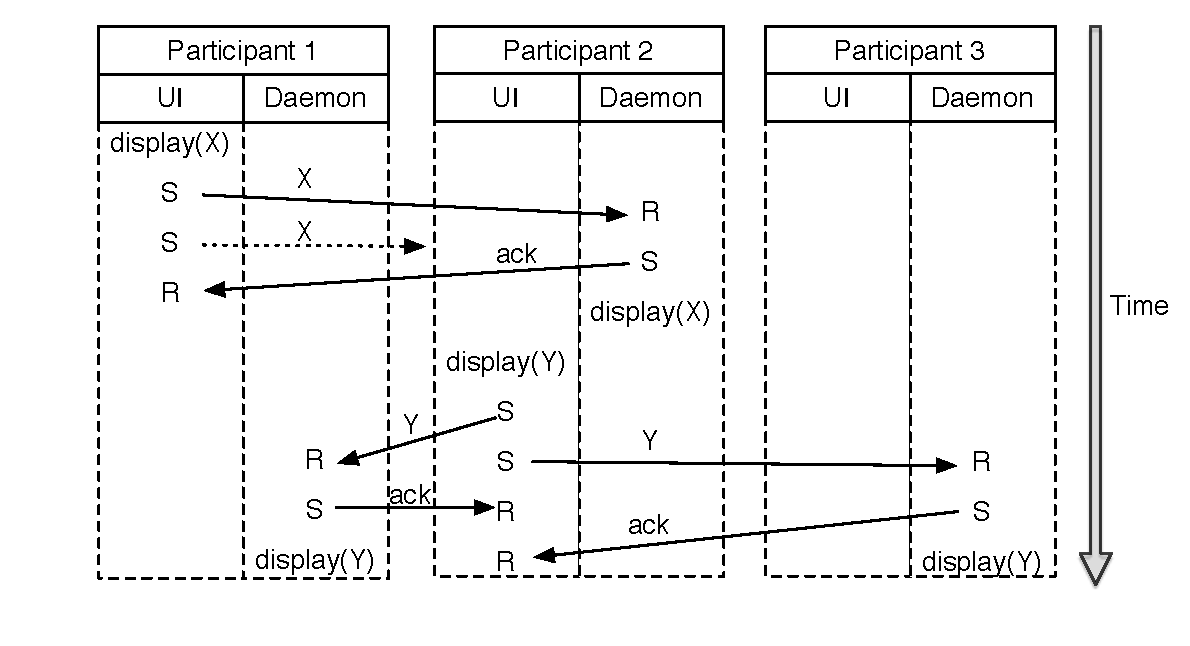
\includegraphics[width=\textwidth] {Figures/ChatServer_AsyncValue}
	\caption{Incorrect execution due to unsafe relaxation of sends during
	broadcast. Dotted arrow represents in-flight message.}
	\label{fig:CS_asend_value}
\end{centering}
\end{figure}

Consider the case where the value is distributed asynchronously. Assume that
there are three participants: $p_1$, $p_2$, and $p_3$. Participant $p_1$ first
types message \cf{X}, which is seen by $p_2$, who in turn types the message
\cf{Y} after sending an acknowledgment. Since there is a causal order between
the message {\codecf X} and {\codecf Y}, $p_3$ must see {\codecf X} followed by
{\codecf Y}. Figure~\ref{fig:CS_asend_value} shows an execution where this is
not the case. In the figure, uninteresting messages have been elided for
clarity. The key observation is that, due to asynchrony, message \cf{X} sent
by the $p_1$ to $p_3$ might be \emph{in-flight}, while the causally dependent
message \cf{Y} sent by $p_2$ reaches $p_3$ out-of-order. This leads to a
violation of the protocol's invariants.

Similarly, it is easy to see that sending acknowledgments message
asynchronously is also incorrect. This would allow a participant that receives
a message to asynchronously send an acknowledgment, and proceed before all
other participants have received the same message. As a result, causal
dependence between messages is lost.

To quantify these issues in a realistic setting, we implemented a group chat
simulator application using a distributed extension of the MultiMLton Standard
ML compiler. We launched three Amazon EC2 instances, each simulating a
participant in the group chat application, with the same communication pattern
described in the discussion above. In order to capture the geo-distributed
nature of the application, participants were placed in three different
availability zones -- EU West (Ireland), US West (Oregon), and Asia Pacific
(Tokyo), resp.

During each run, $p_1$ broadcasts a message \cf{X}, followed by $p_2$
broadcasting \cf{Y}. We consider the run to be successful if the participant
$p_3$ sees the messages \cf{X},\cf{Y}, in that order.  The experiment was
repeated for 1K iterations. We record the time between protocol initiation and
the time at which each participant gets the message \cf{Y}. We consider the
largest of the times across the participants to be the running time. The
results are presented below.

\begin{center}
\begin{tabular}{ | l | r | r |}
	\hline
	\emph{Execution} 					& \emph{Avg.time (ms)} & \emph{Errors} \\
  \hline
	\emph{Sync}								& 1540	\ci{53} &	0 \ci{0} \\
	\emph{Unsafe Async} 			& 520		\ci{17} & 7 \ci{2} \\
	\emph{Safe Async (\rxcml)}	& 533		\ci{13} & 0 \ci{0} \\
  \hline
\end{tabular}
\end{center}

The \emph{Unsafe Async} row describes the variant where both value and
acknowledgment distribution is performed asynchronously; it is three times as
fast as the synchronous variant.  However, over the total set of 1K runs, it
produced seven erroneous executions. The \emph{Safe Async} row illustrates our
implementation, \rxcml, that detects erroneous executions on-the-fly and
remediates them. The results indicate that the cost of ensuring safe
asynchronous executions is quite low for this application, incurring only
roughly 2.5\% overhead above the unsafe version. Thus, in this application, we
can gain the performance benefits and responsiveness of the asynchronous
version, while retaining the simplicity of reasoning about program behavior
synchronously.

\section{Axiomatic Semantics}
\label{sec:axiomatic}

We introduce an axiomatic formalization for reasoning about the relaxed
behaviors of a concurrent message-passing programs with dynamic thread
creation. Not surprisingly, our formulation is similar in structure to
axiomatic formalizations used to describe, for example, relaxed memory
models~\cite{BMM,Sarkar09,Sewell10}.

An \emph{axiomatic execution} is captured by a set of \emph{actions} performed
by each thread and the relationship between them. These actions abstract the
relevant behaviors possible in a CML execution, relaxed or otherwise. Relation
between the actions as a result of sequential execution, communication, thread
creation and thread joins define the dependencies that any sensible execution must
respect. A relaxed execution, as a result of speculation, admits more behaviors
than observable under synchronous CML execution. Therefore, to understand the
validity of executions, we define a \emph{well-formedness} condition that
imposes additional constraints on executions to ensure their observable effects
correspond to correct CML behavior.

We assume a set of $\ThreadClass$ threads, $\ChannelClass$ channels, and
$\ValueClass$ values.  The set of actions is provided below. Superscripts $m$
and $n$ denote a unique identifier for the action.

\begin{mathpar}
\begin{array}{rcll}
\R{Actions} \; \ActionClass{}
	& \coloneqq & b_t 			& \R{(t starts)} \\
	& \mid      & e_t 			& \R{(t ends)} \\
	& \mid      & j_t^mt' 	& \R{(t detects t' has terminated)} \\
	& \mid      & f^m_tt' 	& \R{(t forks a new t')} \\
	& \mid 	    & s_t^mc,v 	& \R{(t sends value v on c)} \\
	& \mid      & r_t^mc   	& \R{(t receives a value v on c)} \\
	& \mid 	    & p_t^mv	 	& \R{(t outputs an observable value v)}
\end{array}

c      ~ \in ~ \ChannelClass ~ \R{(Channels)} \tab
t,t'   ~ \in ~ \ThreadClass ~ \R{(Threads)} \tab
v     ~ \in ~ \ValueClass ~ \R{(Values)} \tab
m,n ~ \in ~ \NumberClass ~ \R{(Numbers)}
\end{mathpar}

\noindent Action $b_t$ signals the initiation of a new thread with identifier
$t$; action $e_t$ indicates that thread $t$ has terminated.  A join action,
$j_t^mt'$, defines an action that recognizes the point where thread $t$ detects
that another thread $t'$ has completed.  A thread creation action, where thread
$t$ spawns a thread $t'$, is given by $f^m_tt'$. Action $s_t^mc,v$ denotes the
communication of data $v$ on channel $c$ by thread $t$, and $r_t^mc$ denotes
the receipt of data from channel $c$.  An external action (e.g., printing) that
emits value $v$ is denoted as $p_t^mv$.  We can generalize these individuals
actions into a family of related actions:
\begin{mathpar}
\begin{array}{lcll}
\ActionClass{r} &=& \{r_t^mc \mid t \in\ThreadClass\} & \R{(Receives)} \\
\ActionClass{s} &=& \{s_t^mc,v \mid t \in\ThreadClass, v\in\ValueClass\} & \R{(Sends)} \\
\ActionClass{c} &=& \ActionClass{s} \cup \ActionClass{r} & \R{(Communication)} \\
\ActionClass{o} &=& \{p_t^mv		 \mid	t \in\ThreadClass,v\in\ValueClass\} & \R{(Observables)} \\
\end{array}
\end{mathpar}

\noindent {\bf Notation.} We write $T(\alpha)$ to indicate the thread in which
action $\alpha$ occurs, and write $\,V(s_t^mc,v)$ to extract the value $v$
communicated by a send action. Given a set of actions $\ActionSet \in
2^\ActionClass{}$, $\ActionSet_x = \ActionSet \cap \ActionClass{x}$, where
$\ActionClass{x}$ represents one of the action classes defined above.

\begin{definition}[Axiomatic Execution]
An axiomatic execution is defined by the tuple $\E \coloneqq \Exec$ where:
\begin{itemize}
\item $\program$ is a program.
\item $\ActionSet$ is a set of actions.
\item $\po \; \subseteq \ActionSet \times \ActionSet$ is the program order,
  a disjoint union of the sequential actions of each thread (which is a
  total order).
\item $\co \; \subseteq (\ActionSet_s \times \ActionSet_r) \cup (\ActionSet_r
	\times \ActionSet_s)$ is the communication order which is a symmetric
	relation established between matching communication actions (i.e., $\alpha
	\co \beta \implies \beta \co \alpha$). Moreover, a send and its matching
	receive must operate over the same channel (i.e., $s_t^mc,v \co r_{t'}^n{c'}
	\implies c = c'$).
\end{itemize}
\label{defn:exec}
\end{definition}

Additionally, there is an obvious ordering on thread creation and execution, as
well as the visibility of thread termination by other threads:

\begin{definition}[Thread Dependence]
\label{def:thr_dep}
If $\alpha = f_t^mt'$ and $\beta = b_{t'}$ or  $\alpha = e_t$ and $\beta = j_{t'}^mt$
then $\alpha \td \beta$ holds.
\end{definition}


\begin{definition}[Happens-before relation]
\label{def:hb}
The \textit{happens-before} order of an execution is the transitive closure of
the union of program order, thread dependence order, and actions related by
communication and program order:
\begin{mathpar}
\begin{array}{lll}
\hb & = & (\po \cup \td \cup \\
    &   &  \{ (\alpha,\beta)\ |\ \alpha \co \alpha' \wedge \alpha' \po \beta \}\ \cup \\
    &   &  \{ (\beta,\alpha)\ |\ \beta \po \alpha' \wedge \alpha' \co \alpha \})^+
\end{array}
\end{mathpar}
\end{definition}

\noindent For any two actions $\alpha,\beta \in \ActionSet$, if $\alpha \nbihb
\beta$, then $\alpha$ and $\beta$ are said to be \textit{concurrent} actions.
Importantly, our happens-before relation defines a preorder. A preorder is a
reflexive transitive binary relation. Unlike partial orders, preorders are not
necessarily anti-symmetric, i.e. they may contain cycles.

\begin{definition}[Happens-before Cycle]
A cycle exists in a happens-before relation if for any two actions
$\alpha, \beta$ and $\alpha \hb \beta \hb \alpha$.
\end{definition}

\lstset{numbers=none}
\begin{figure}
\begin{lstlisting}
(* current thread is t1 *)
val t2 = spawn (fn () => recv c2; print "2"; recv c1)

val t3 = spawn (fn () => send(c2,v2); print "3"; recv c2)

val _ = send(c1,v1)
val _ = print "1"
val _ = send(c2,v2)
\end{lstlisting}
\caption{A CML Program with potential for mis-speculation.}
\label{code:simple}
\end{figure}
\lstset{numbers=left,numberstyle=\tiny,stepnumber=1,frame=single}

\begin{figure}
\begin{minipage}{0.5\textwidth}
\subfigure[Well-formed execution]{\label{fig:well}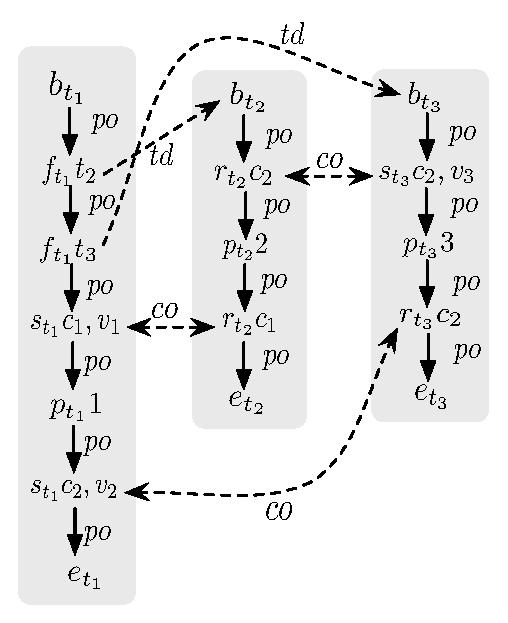
\includegraphics[width=1\textwidth]{Figures/AxiomaticExecution}}
\end{minipage}
\hfill
\begin{minipage}{0.5\textwidth}
\subfigure[Ill-formed execution]{\label{fig:ill}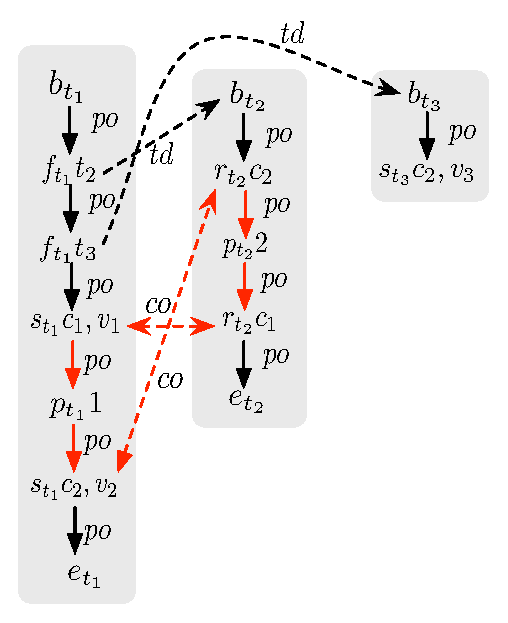
\includegraphics[width=1\textwidth]{Figures/AxiomaticExecution-1}}
\end{minipage}
\caption{Potential axiomatic executions of the CML program presented in Figure~\ref{code:simple}.}
\label{fig:pgm_and_execs}
\end{figure}

We provide an example to illustrate these definitions and to gain an insight
into erroneous executions that manifest as a result of speculative
communication. Consider the simple CML program (Figure~\ref{code:simple}) which
shows a simple CML program and two possible executions
(Figure~\ref{fig:pgm_and_execs}). The execution in Figure~\ref{fig:well}
imposes no causal dependence between the observable actions (i.e., print
statements) in $t_2$ or $t_3$; thus, an interleaving derived from this
execution may permute the order in which these statements execute. All
interleavings derivable from this execution correspond to valid CML behavior.

In contrast, the execution depicted in Figure~\ref{fig:ill}, exhibits a
happens-before cycle between $t_1$ and $t_2$, through a combination of program
and communication order edges. \emph{Such cyclic dependences never manifest in
any correct CML execution}. Cyclic dependences may however manifest when
synchronous sends are speculatively discharged asynchronously. We must
therefore strengthen our notion of correct executions to discard those that
contain such cycles.

To do so, we first note that the semantics as currently presented is concerned
only with actions that introduce some form of causal dependence either within a
thread (via program order) or across threads (via thread dependence or
communication order). However, a real program also does computation, and
reasoning about an execution's correctness will require us to specify these
actions as well. To facilitate this reasoning, we abstract the intra-thread
semantics, and parameterize our definition of an axiomatic execution accordingly.

\subsubsection{Intra-thread semantics} The intra-thread semantics is abstracted
in our formulation via a labeled transition system.  Let $\intrastate$ denote
the intra-thread state of a thread; its specific structure is not interesting
for the purposes of the axiomatic definition. A labeled transition between
intra-thread states is captured by the relation, $\intratrans{.} \subseteq
\intrastate \times \intralabel \times \intrastate$, given to each thread $t \in
\ThreadClass$. The transition labels are in the set $\intralabel =
(\ActionClass{} \setminus \ActionClass{r}) \cup (\ActionClass{r} \times
\ValueClass) \cup \{\tau\}$.  Thus, a thread can either take a global action
step (e.g., creating another thread, performing a send action, ending a thread,
etc.), execute a \emph{silent} thread-local computation (denoted by label
$\tau$), or execute a receive action that receives the value associated with
the label. The requirements on the intra-thread semantics are:

\begin{itemize}
\item $\intratrans{.}$ can only relate states belonging to the same thread.
\item there is an initial state \ready: no transition leads to it,
	and a thread $t$ steps from it if and only if it emits a begin action $b_t$.
\item there is a final state \done: a thread leads to it if and only if it
	emits an end action $e_t$ and no transition leads from it.
\end{itemize}

\begin{definition}[Intra-trace]
\label{def:intra-trace}
Let $tr = \bar{\alpha}$ be a sequence of actions in set $\ActionSet$, and
$\co$ be a communication order on $\ActionSet$. Given a thread
$t \in \ThreadClass$ in a program $\program$, $tr$ is a valid intra-trace for
$t$ if there exists a set of states $\{\delta_0, \delta_1, \ldots \}$, and a
set of labels $\bar{l} = \{l_0, l_1,\ldots\}$ such that:
%
\begin{itemize}
\item for all $\alpha_i \in \bar{\alpha}, T(a) = t$
\item $\delta_0$ is the initial state \ready
\item for all $0 \leq i, \delta_{i} \intratrans{l_i} \delta_{i+1}$
\item the projection $\bar{\beta}$ of $\bar{l}$ to non-silent labels is such
	that $\beta_i = (\alpha_i, V(\gamma_i))$ if $\alpha_i \in \ActionSet_r$ and
	$\alpha_i \co \gamma_i$, or $\beta_i = \alpha_i$ otherwise.

\end{itemize}
\end{definition}

\noindent We write $\intraTraceSet[t]$ set of such pairs $(tr,\co)$ for
$\program$.

\begin{definition}[Well-formed Execution]
\label{def:well-formed}
An execution $E \coloneqq \Exec$ is well-formed if the following
conditions hold:
%
\begin{enumerate}
\item Intra-thread consistency: for all threads $t \in \ThreadClass,
	\;(\restrict{\po}{t}, \co) \in \intraTraceSet[t]$
\item Happens-before correctness: The happens-before relation $\hb$ constructed
	from $E$ has no cycles.
\item Observable correctness: Given $\alpha  \in \ActionSet_{o}$ and  $\beta
	\in \ActionSet_{c}$ if $\beta \hb \alpha$ then there exists $\beta' \in
	\ActionSet_{c}$ s.t. $\beta \co \beta'$.
\end{enumerate}
\end{definition}

For an axiomatic execution $\E \coloneqq \Exec$ to be well-formed, the actions,
program order and communication order relations must have been obtained from a
valid execution of the program $\program$ as given by the intra-thread
semantics defined above (1). As we noted in our discussion of
Figure~\ref{fig:pgm_and_execs}, no valid execution of a CML program may involve
a cyclic dependence between actions; such dependencies can only occur because
of \emph{speculatively} performing what is presumed to be a synchronous send
operation (2).

Finally, although the relaxed execution might speculate, i.e., have a send
operation transparently execute asynchronously, the observable behavior of such
an execution should mirror some valid non-speculative execution, i.e., an
execution in which the send action was, in fact, performed synchronously.  We
limit the scope of speculative actions by requiring that they complete (i.e.,
have a matching recipient) before an observable action is performed (3).
Conversely, this allows communication actions not preceding an observable
action to be speculated upon. Concretely, a send not preceding an externally
visible action can be discharged asynchronously. The match and validity of the
send needs to be checked only before discharging the next such action. This is
the key idea behind our speculative execution framework.

\subsubsection{Safety.} An axiomatic execution represents a set
of interleavings, each interleaving defining a specific total order that is
consistent with the partial order defined by the execution\footnote{Two
ordering relations $P$ and $Q$ are said to be \textit{consistent} if
$\forall x,y, \neg(xPy \conj yQx)$.}.  The well-formedness conditions of an
axiomatic execution implies that any observable behavior of an interleaving
induced from it must correspond to a synchronous CML execution. The
following two definitions formalize this intuition.

\begin{definition}[Observable dependencies]
\label{def:od}
In a well-formed axiomatic execution $\E \coloneqq \Exec$, the observable
dependencies $\ActionSet_{od}$ is the set of actions that precedes (under
$\hb$) some observable action, i.e., $\ActionSet_{od} = \{\alpha \ALT \alpha \in
\ActionSet, \beta \in \ActionSet_{o}, \alpha \hb \beta\}$.
\end{definition}

\begin{definition}[$\cml$ Execution]
\label{def:cml}
Given a well-formed axiomatic execution $\E \coloneqq \Exec$, the pair $(\E,
\toto)$ is said to be in $\cml(\program)$ if $\toto$ is a total order on
$\ActionSet_{od}$ and $\toto$ is consistent with $\hb$.
\end{definition}

In the above definition, an interleaving represented by $\toto$ is only possible
since the axiomatic execution is well-formed, and thereby does not contain a
happens-before cycle.

\begin{lemma}
\label{lem:toto_hb}
If a total order $\toto$ is consistent with $\hb$, then $\hb$ does not contain
a cycle involving actions in $\ActionSet_{od}$.
\end{lemma}

%% \begin{proof}
%% Assume $\alpha \hb \beta \hb \alpha$, then either $\alpha \toto \beta$ or
%% $\beta \toto \alpha$. If $\alpha \toto \beta$, then pick $\beta \hb \alpha$ and
%% show that $\toto$ is not consistent with $\hb$. Similarly for the other case.
%% \end{proof}

Next, we show that a well-formed axiomatic execution respects the safety
property of non-speculative execution of a CML program. When a CML program
evaluates non-speculatively, a thread performing a communication action is
blocked until a matching communication action is available. Hence, if
$(\Exec,\toto) \in \cml(\program)$, and a communication action $\alpha$ on a
thread $t$ is followed by an action $\beta$ on the same thread, then it must be
the case that there is a matching action $\alpha \co \alpha'$ that
happened before $\beta$ in $\toto$. This is captured in the following theorem.

\begin{theorem}
Given a CML execution $(\E, \toto) \in \cml(\program)$, $\forall \alpha,\beta$
such that $\alpha \in \ActionClass{c}, T(\alpha) = T(\beta), \alpha \toto \beta$,
there exists an action $\alpha \co \alpha'$ such that $\alpha' \toto
\beta$.
\end{theorem}
\begin{proof}
Let $\E \coloneqq \Exec$. First, we show that $\alpha' \in \ActionSet$. Since
$\alpha \toto \beta$, $\alpha \in \ActionSet_{od}$, by
Definition~\ref{def:cml}. By Definition~\ref{def:od}, there exists some $\gamma
\in \ActionSet_o$ such that $\alpha \hb \gamma$. Since $\E$ is well-formed and
$\alpha \hb \gamma$, by Definition~\ref{def:well-formed}, there exists an
$\alpha' \in \ActionSet$ such that $\alpha \co \alpha'$.

Next, we show that $\alpha' \in \ActionSet_{od}$. By Definition~\ref{def:hb},
$\alpha' \co \alpha \hb \gamma$ implies $\alpha' \hb \gamma$. Hence, $\alpha'
\in \ActionSet_{od}$, and is related by $\toto$. Finally, since $T(\alpha) =
T(\beta)$ and $\alpha \toto \beta$, $\alpha \po \beta$. And, $\alpha' \co
\alpha \po \beta$ implies $\alpha' \hb \beta$. By Lemma~\ref{lem:toto_hb} and
Definition~\ref{def:cml}, $\alpha' \toto \beta$.
\end{proof}

\section{Operational Semantics}

\begin{figure}
\begin{minipage}[t]{\columnwidth}
\begin{smathpar}
\begin{array}{lclcl}
e & \in & {\tt Exp} & := 		& v \ALT x \ALT e \; e \ALT \chan() \ALT \print(e) \ALT \spawn(e) \\
	&			&						& \ALT 	&	\send(e,e) \ALT 	\recv(e) \ALT \join(e)\\
v & \in & {\tt Val} & := 		& \unit \ALT c \ALT \lambda\,x.e \ALT t \\
\end{array}
\end{smathpar}
\end{minipage}
%
\begin{minipage}[t]{\columnwidth}
\begin{smathpar}
\begin{array}{lcl}
E & := 		& \bullet \ALT E\;e \ALT v\;E \ALT \print(E) \\
  & \ALT 	& \spawn(E) \ALT \send(E,e) \ALT \send(c,E) \\
	& \ALT	& \recv(E) \ALT \join(E)
\end{array}
\end{smathpar}
\end{minipage}

\begin{minipage}[t]{\columnwidth}
\begin{smathpar}
\begin{array}{lclcl}
c & \in & {\tt ChannelId}\\
\alpha,\beta 	& \in & {\tt Action} & := & \ActionClass\ \ALT (\alpha,\beta) \ALT\ \tau_t \ALT \commit{\program}{\trace}\\
\ActionSoup 	& \in & {\tt SendSoup}		& := & \ActionClass{s}\\
\localstate 	& \in & {\tt LocalState} & := & e \ALT \readyOp{e} \ALT \doneOp \\
t 						& \in & {\tt ThreadId}\\
\thread 			& \in & {\tt Thread} 				& := & (t,\localstate) \\
\threadsoup 	& \in & {\tt ThreadSoup}		& := & \emptyset \ALT \thread \;\|\; \threadsoup\\
\langle \threadsoup,\ActionSoup \rangle	& \in & \ProgramState
\end{array}
\end{smathpar}
\end{minipage}
\caption{Syntax and states for the relaxed execution semantics of a subset of CML.}
\label{sem:rxcml_op_syntax}
\end{figure}

\begin{figure}
\begin{smathpar}
\begin{array}{cl}

\RULE
{\\ }
{\PrgState{(\lambda\,x.e) v}{\ActionSoup}
\intertrans{\tau_t}
\PrgState{e[x/v]}{\ActionSoup}} & \rulelabel{App} \\ \\

\RULE
{c \;\; \fresh \;\;\; }
{\PrgState{\chan()}{\ActionSoup}
\intertrans{\tau_t}
\PrgState{c}{\ActionSoup}} & \rulelabel{Chan} \\ \\

\RULE
{\\
}
{\langle (t,\readyOp{e}) \;\|\; \threadsoup, \ActionSoup \rangle
 \intertrans{b_t}
 \langle (t,e) \;\|\; \threadsoup, \ActionSoup \rangle} & \rulelabel{Begin} \\ \\

\RULE
{}
{\langle (t,v) \;\|\; \threadsoup,\ActionSoup \rangle
 \intertrans{e_t}
 \langle (t,\doneOp) \;\|\; \threadsoup, \ActionSoup \rangle} & \rulelabel{End} \\ \\

\RULE
{}
{\PrgState{\spawn\,e}{\ActionSoup}
\intertrans{f_t^it'}
\langle (t,\opIntraState{t'}) \;\|\; (t',\readyOp{e}) \;\|\; \threadsoup, \ActionSoup \rangle} & \rulelabel{Spawn} \\ \\

\RULE
{}
{\langle (t,\opIntraState{\join\,t'}) \;\|\; (t',\doneOp) \;\|\; \threadsoup, \ActionSoup \rangle
 \intertrans{j_t^it'}
 \langle (t,\opIntraState{\unit}) \;\|\; (t',\doneOp) \;\|\; \threadsoup, \ActionSoup \rangle} & \rulelabel{Join} \\ \\

\RULE
{\\}
{\PrgState{\print\,v}{\ActionSoup} \intertrans{p_t^iv}
\PrgState{\unit}{\ActionSoup}} & \rulelabel{Print} \\ \\

\RULE
{\alpha = s_t^ic,v}
{\PrgState{\send(c,v)}{\ActionSoup}
 \intertrans{\alpha}
 \PrgState{\unit}{\ActionSoup \cup \{\alpha\}}} & \rulelabel{Send} \\ \\

\RULE
{\alpha = r_t^ic \;\;\; \beta = (s_{t'}^jc,v) \in \ActionSoup}
{\PrgState{\recv\,c}{\ActionSoup}
\intertrans{(\alpha,\beta)}
\PrgState{v}{\ActionSoup \setminus \beta}} & \rulelabel{Recv} \\ \\

\RULE
{\wf{(\program,\trace)}}
{\langle\threadsoup,\ActionSoup\rangle
\intertrans{\commit{\program}{\trace}}
\langle\threadsoup,\ActionSoup\rangle} & \rulelabel{Commit}

\end{array}
\end{smathpar}
\caption{A relaxed execution operational semantics for a subset of CML.}
\label{fig:op_semantics}
\end{figure}

The axiomatic semantics provides a declarative way of reasoning about
executions. However, it is unclear how to use this semantics to
\emph{execute} a CML program that performs the sends asynchronously
while ensuring that the observable behaviors correspond to a
synchronous execution of the program; that is, how we can we ensure
that implementations produce relaxed executions that always conform to
a CML execution in the sense of Definition~\ref{def:cml}?  In this
section, we present an operational definition of a relaxed execution
as a labeled transition system that allows us to express the
constraints necessary to prevent non-CML observable behaviors.

The operational machine, $\rel$, takes as its input an operational execution,
which is composed of a program, and a trace $\trace$ of \emph{operational
actions}. It evaluates the program according to the trace, by manipulating a
\emph{send soup}, an unordered set into which pending sends are added
asynchronously.  Informally, we can think of the trace as a history or log of
actions we wish to perform; the machine either accepts the trace, if executing
the actions found in the trace using the reduction rules leads to a CML
execution (as defined by Definition~\ref{def:cml}), or gets stuck otherwise. An
operational action $\alpha \in \ActionClass{op}$ is either:

\begin{itemize}

\item an action in $\ActionClass{} \setminus \ActionClass{r}$.
\item a pair in $\ActionClass{r} \times \ActionClass{s}$ where each receive
	action is paired up with the matching send action on the same channel,
\item a \emph{silent} action $\tau_t$ indexed by a thread identifier that
  indicates the evaluation of a computation step (e.g., a function call).
\item a \emph{commit} action $\commit{\program}{\trace}$ that checks whether
  the machine state is well-formed in the sense of
  Definition~\ref{def:well-formed}.  Intuitively, a well-formed machine
  state is one that could have been reached if all \cf{send} operations
  were executed synchronously.

\end{itemize}

\begin{definition}[Operational Execution]
An operational execution is a pair $(\program,tr)$, where $\program$ is a
program and $tr \in \bar{\ActionClass{op}}$, and there are no duplicates in
$tr$.
\end{definition}

The semantics used to interpret the trace is given in
Figure~\ref{fig:op_semantics}.  The program state is composed of a tuple
with $\threadsoup$ representing the pool of concurrently executing threads
and a collection of unmatched send actions $\ActionSoup$. Each thread in
$\threadsoup$ is a tuple with a thread id and a local state.  This state is
either an initial state $\readyOp{e}$ containing the expression that will
be evaluated by this thread, or a completed state $\doneOp$, or the
expression being evaluated by this thread.  Each state transition is affixed
with an action drawn from the trace that is used by the machine to determine
which rule to apply, as we describe below.

The source language contains function abstraction, application, first-class
channels, a thread creation operation ({\sf spawn}), message-passing
primitives on these channels, and a {\sf print} statement to capture an
observable action.  Reductions are labeled with operational actions. Rules
{\sc App} and {\sc Chan} represent silent (thread-local) actions.  The {\sc
  Spawn} rule creates a new thread with the initial local state
$\readyOp{e}$. Rule {\sc Begin} initiates execution of the thread from its
initial state.  A thread moves to the $\doneOp$ local state once the
expression being evaluated is reduced to a value (Rule {\sc End}). The
completed thread remains in the thread pool so that other threads may also
join on it.  A thread can wait on another thread's completion by joining on
its thread identifier. The calling thread is paused until the joined thread
moves to the final local state $\doneOp$ (Rule {\sc Join}).

The {\sc Send} rule adds the associated send action $\alpha$ into
$\ActionSoup$, the collection of pending send actions, and allows
execution to proceed.  Thus, this rule captures asynchronous behavior.
The transition defined by the {\sc Recv} has a label defined as a
pair, consisting of the receive action $\alpha$ and an unmatched send
action $\beta$, which belongs to the send pool. The receiver thread
consumes the value contained in the send action, and removes the
action from $\ActionSoup$.  An observable action (rule {\sc Print}) is
evaluated only if the trace emits a print action; this rule exists
primarily to allow us to reason about equivalence of observable
behaviors as we describe below.  Finally, we define a commit rule
(rule {\sc Commit}) that checks whether the interleaving generated
thus far corresponds to a sensible CML execution, i.e., whether the
interleaving exhibits a behavior that could have been observed if all
\cf{send} operations executed thus far were evaluated synchronously.
It uses an operator {\sf WF} defined below.

\begin{definition}[$\rel$ execution]

Given a trace $\trace = \bar{\beta}.\commit{\program}{\bar{\beta}}$
terminating in a commit action, an operational execution $(\program,
\trace)$ is a \emph{relaxed} execution ($\rel(\program,\trace)$) if there
exists an ordered sequence $\bar{\delta} \in \ProgramState$ satisfying the
following:

\begin{itemize}
\item $\delta_0 = \langle (t_0,\readyOp{\program}),\emptyset\rangle$ for some
unique thread identifier $t_0$.
\item for all $\alpha_i \in \trace$, there exists $\delta_{i}$,
  $\delta_{i+1} \in \bar{\delta}$ such that $\delta_{i} \intertrans{\alpha_i}
  \delta_{i+1}$.
\end{itemize}
\end{definition}

\noindent Clearly, not every operational execution $(\program,\mathit{tr})$ is a
relaxed execution.  Consider the following program $\program$:

\begin{code}
fun main () =
let val c = channel()
in print (send(c,v); recv c)
end
\medskip
\end{code}

\noindent with trace
  \[ \trace = b_t.s_t^ic,v.(r_t^jc;\;s_t^ic,v).p_t^kv.e_t \]

\noindent where silent transitions have been elided.  When suffixed with a
commit action $\commit{\program}{\trace}$, the resulting behavior would not
be accepted by the semantics, since no synchronous execution of the program
would result in a match of the \cf{send} operation with a \cf{recv} action
on the same thread.  The prohibition of such behavior is encapsulated within
the definition of well-formedness found in the antecedent of the {\sc
  Commit} rule that we formalize below.

We reason about sensible (well-formed) relaxed executions by
transforming them into an equivalent axiomatic one.  A well-formed
$\rel$ execution is one whose corresponding axiomatic execution is
well-formed. Since an axiomatic semantics is parameterized by an
intra-thread semantics, we first provide a translation that produces
this semantics given the transitions defined by the operational
semantics.

\begin{definition}[Intra-thread semantics]
\label{def:intra-rel}
Given a program $\program$, let
\[\intrastate \coloneqq \ready \ALT \done \ALT e\]
where $e \in \program$. For each labeled transition of the form $\langle
(t,s) \| \threadsoup, \ActionSoup \rangle \intertrans{\alpha} \langle (t,s') \|
\threadsoup', \ActionSoup' \rangle$, where $\alpha \neq
\commit{\program}{\trace}$, we define $\delta \intratrans{\beta} \delta'$,
where $\delta, \delta' \in \intrastate$ such that:
\begin{itemize}
	\item if $s = \readyOp{e}$, then $\delta = \ready$, otherwise, $\delta = s$.
	\item if $s' = \doneOp$, then $\delta' = \done$, otherwise $\delta' = s'$
	\item if $\alpha = ((r_t^ic),\,(s_{t'}^jc,v))$ then $\beta = (r_t^ic;\,v)$
  \item if $\alpha = \tau_t$ then $\beta = \tau$
  \item otherwise, $\alpha = \beta$
\end{itemize}

\end{definition}

\begin{definition}[$\opax$ operator]
Let $\E_{o} = (\program, tr)$ be an operational execution. $\opax$ is defined
as $\opax(\E_{o}) = \Exec$ parameterized with the intra-thread semantics
$\intratrans{}$ (Definition~\ref{def:intra-rel}), where

\begin{itemize}
\item $\ActionSet$ is a set of non-silent, non-commit actions in $tr$.
\item for all $\alpha,\beta \in \ActionSet$, $\alpha \po \beta$ iff $T(\alpha)
	= T(\beta)$ and $\alpha$ precedes $\beta$ in $tr$.
\item for all pairs $(a,b)$ such that $a = r_t^ic$ and $b = s_{t'}^jc,v$, $a
	\co b ∧ b \co a$
\end{itemize}
\end{definition}

For perspicuity, in the definition of $\ActionSet$ and $\po$ above, a receive
operational action $(a,b) \in \ActionClass{op}$ is simply treated as $a \in
\ActionClass{r}$.

\begin{definition}[Well-formed $\rel$ execution]
\label{def:well-formed-rel}
Let $\E_o = (\program,tr) \in \rel(\program)$ be an operational execution. If
the axiomatic execution $\E_{ax} = \opax(\E_o)$ is well-formed, then $\E_o$ is
well-formed.
\end{definition}

\begin{theorem}
If $E_o = (\program,\trace)$ and $\wf{E_o}$, then\\ \mbox{$(\opax(\E_o), \toto) \in
\cml(\program)$}.
\end{theorem}

\begin{proof}
We provide a witness for $\opax(\E_o)$ via a generative operator $\opaxGen$
(Definition~\ref{def:opaxGen_ap}) such that $\opaxGen(\E_o)$ is an axiomatic
execution (Theorem~\ref{thm:g_ax_ap}) and $\opaxGen(\E_o) = \opax(\E_o)$
(Theorem~\ref{thm:g_eq_t_ap}). We then prove that if $\E_o$ is well-formed,
then $\opaxGen(\E_o)$ is well-formed (Lemma~\ref{lem:wf_opaxGen_ap}). Since
$\opaxGen(\E_o)$ is well-formed, by definition~\ref{def:cml_ap} and
theorem~\ref{thm:g_eq_t_ap}, $(\opax(\E_o), \toto) \in \cml(\program)$.
\end{proof}

\begin{definition}[$\opaxGen$ operator]
\label{def:opaxGen_ap}
Let $\E_{op} = (\program,\trace) \in \rel(\program)$ be a well-formed
operational execution. $\opaxGen(\E_{op})$ is an axiomatic execution
parameterized with the intra-thread semantics $\intratrans{}$
(definition~\ref{def:intra-rel_ap}) defined as follows:
\begin{itemize}
\item $\opaxGen(\program,\emptyset) = \langle \program, \emptyset, \emptyset,
	\emptyset \rangle$
\item If $\opaxGen(\program,\bar{\alpha}) = \Exec$ , then $\E_{ax} =
	\opaxGen(\program,\bar{\alpha}.\beta)$ defined as follows:
	\begin{enumerate}
	\item if $\beta = \tau_t$ or $\beta = \commit{\program}{\bar{\alpha}}$, then
		$\E_{ax} = \Exec$
	\item if $\beta \notin (\ActionClass{r} \times \ActionClass{s})$, then $\E_{ax} =
		\langle \program, \ActionSet \cup \{\beta\}, \po \cup~ \{\gamma \po \beta \ALT
		\gamma \in \ActionSet, T(\gamma) = T(\beta)\}, \co \rangle$
	\item if $\beta = (\gamma,\,\zeta)$, then $\E_{ax} = \langle \program,
		\ActionSet \cup \{\gamma\}, \po \cup~ \{\eta \po \gamma \ALT \eta \in
		\ActionSet, T(\eta) = T(\gamma)\}, \co \cup~ \{\gamma \co \zeta, \zeta \co
		\gamma\} \rangle$
	\end{enumerate}
\end{itemize}
\end{definition}

\begin{theorem}
\label{thm:g_ax_ap}
Let $\E_{op} = (\program,\trace) \in \rel(\program)$ be an operational
execution. Then, $\opaxGen(\E_{op})$ is an axiomatic execution.
\end{theorem}
\begin{proof}
We show that the quadruple generated by the $\opaxGen$ operator satisfies the
conditions necessary for an axiomatic execution (Definition~\ref{def:exec_ap}).
In particular, (1) $\ActionSet$ is composed of actions from $\ActionClass{}$,
(2) $\po$ is a disjoint total order on actions belonging to each thread. (3)
$\co$ is a symmetric relation and relates actions belonging to the same
channel. We show these conditions hold by induction on $\left|{\trace}\right|$.

The base case is if $\E_{op} = (\program,\emptyset) \in \rel(\program)$, then
$\opaxGen(\E_{op})$ is an axiomatic execution. If the trace is empty, then
$\opaxGen(\E_{op}) = \Exec$. Here, $\program$ is a valid program. $\ActionSet$,
$\po$, and $\co$ are empty. Hence, the conditions defined under
Definition~\ref{def:exec_ap} trivially hold.

Assume $\opaxGen(\program,\bar{a})$ is an axiomatic execution.  We show that
$\opaxGen(\program,\bar{a}.b)$ is an axiomatic execution, where
$b \in \ActionClass{op}$. If $b$ is a silent action or a commit action
(Definition~\ref{def:opaxGen_ap}.1), then $\opaxGen(\program,\bar{a}.b)
= \opaxGen(\program,\bar{a})$.

Let $b \notin (\ActionClass{r} \times \ActionClass{s})$. Then $b \in
\ActionClass{}$ (Definition~\ref{def:op_act_ap}). In this case
(Definition~\ref{def:opaxGen_ap}.2), $\opaxGen$ operator adds $b$ to
$\ActionSet$ and adds $\po$ edges from all actions $\alpha \in \ActionSet$ such
that $T(\alpha) = T(b)$ to $b$ (preserving the total order). $\co$ is not
modified. By the induction hypothesis, $\opaxGen(\program,\bar{a}.b)$ is an
axiomatic execution.

Let $b = (\alpha,\beta)$. $\alpha \in \ActionClass{r}, \beta \in
\ActionClass{s}$ (Definition~\ref{def:op_act_ap}).   In this case, by
Definition~\ref{def:opaxGen_ap}.3, $\opaxGen$  adds $\alpha$ to $\ActionSet$,
and introduces $\po$ edges from all actions in $\ActionSet$ that belong to the
thread $T(\alpha)$ to $\alpha$ (preserving the total order). $\co$ is extended
with $\{\alpha \co \beta, \beta \co \alpha\}$. By the induction hypothesis,
$\co$ is a symmetric relation. By Definition~\ref{def:op_act_ap},
$\alpha$ and $\beta$ operate on the same channel. Thus,
$\opaxGen(\program,\bar{a}.b)$ is an axiomatic execution.
\end{proof}

\begin{theorem}
\label{thm:g_eq_t_ap}
Given $\E_o = (\program,\trace) \in \rel(\program)$, $\opax(\E_o) =
\opaxGen(\E_o)$.
\end{theorem}
\begin{proof}
By theorem~\ref{thm:g_ax_ap}, $\opaxGen(\E_o)$ is an axiomatic
execution. We need to show that each component in the axiomatic execution
defined by $\opax$ and generated by $\opaxGen$ are the same.  Both operators
use the same program $\program$ and set of actions $\ActionSet$ from $\E_o$.

%% For the set of actions $\ActionSet$, $\opax$ includes only non-silent, non-commit actions
%% (Definition~\ref{def:opax_ap}.1), while $\opaxGen$ does not include the silent
%% and commit actions (definition~\ref{def:opaxGen_ap}.1).

$\opax$ defines a $\po$ relation between actions $\alpha$ and $\beta$ iff
$T(\alpha) = T(\beta)$ and $\alpha$ precedes $\beta$ in the trace
(Definition~\ref{def:opax_ap}.1).  Assume that the operational trace is
$\trace = \bar{\alpha}.\beta$.  For any $\gamma$ such that $T(\gamma) =
T(\beta)$, $\gamma \in \bar{\alpha}$, $\gamma$ belongs to the action set
$\ActionSet$ of
$\opaxGen(\program,\bar{\alpha})$. Definition~\ref{def:opaxGen_ap}.2 and
\ref{def:opaxGen_ap}.3 add a $\po$ edge from such a $\gamma$ to $\beta$.

Definition~\ref{def:opax_ap}.3 defines $\co$ such that for all pairs
$(\alpha,\beta)$ in \emph{tr}, $\alpha \co \beta$ and $\beta \co \alpha$.
$\opaxGen$ extends $\co$ in a similar fashion
(Definition~\ref{def:opaxGen_ap}.3).
\end{proof}

\begin{lemma}
\label{lem:wf_opaxGen_ap}
Let $\E_o = (\program,\trace) \in \rel(\program)$. If $\E_o$ is well-formed,
then $\opaxGen(\E_o)$ is well-formed.
\end{lemma}
\begin{proof}
Since $\E_o$ is well-formed, $\opax(\E_o)$ is a well-formed axiomatic execution
(by Definition~\ref{def:well-formed-rel_ap}). By Theorem~\ref{thm:g_eq_t_ap},
$\opax(\E_o) = \opaxGen(\E_o)$. Hence, $\opaxGen(\E_o)$ is a well-formed
axiomatic execution.
\end{proof}


\newcommand{\qed}{\nobreak \ifvmode \relax \else
      \ifdim\lastskip<1.5em \hskip-\lastskip
      \hskip1.5em plus0em minus0.5em \fi \nobreak
      \vrule height0.75em width0.5em depth0.25em\fi}

\newcommand{\scc}{\psi_{\sf sc}}
\newcommand{\ccc}{\psi_{\sf cc}}
\newcommand{\ecc}{\psi_{\sf ec}}
\newcommand{\rcc}{\psi_{\sf rc}}
\newcommand{\mavc}{\psi_{\sf mav}}
\newcommand{\rrc}{\psi_{\sf rr}}

\newcounter{hno}
\newcounter{gno}
\renewenvironment{proof}{\setcounter{hno}{0}\setcounter{gno}{0}
  \emph{Proof.}}{}
\newcommand{\npp}{\thehno \stepcounter{hno}}
\newcommand{\mpp}{\thegno \stepcounter{gno}}

\newcommand{\stretcharraybig}{\renewcommand*{\arraystretch}{1.25}}
\newcommand{\cureff}{\hat{\eta}}
\newcommand{\eff}{\eta}
\newcommand{\cv}{\psi}
\newcommand{\eid}{{\iota}}
\newcommand{\ObjType}{{\sf ObjType}}
\newcommand{\AbsType}{{\sf AbsType}}
\newcommand{\dom}{{\sf dom}}
\newcommand{\DtLib}[1]{\mathbb{D}(#1)}
\newcommand{\DtLibZ}{\mathbb{D}}
\newcommand{\Ops}{\Lambda}
\newcommand{\Ctrts}{\Psi}
\newcommand{\true}{\N{\textsf{true}}}

\newcommand{\N}[1]{{\normalfont #1}}
\newcommand{\ObjZ}{\N{\textsf{Obj}}}
\newcommand{\Obj}[1]{\N{\textsf{Obj}_{#1}}}
\newcommand{\ReplID}{\mathtt{ReplID}}
\newcommand{\SessID}{\mathtt{SessID}}
\newcommand{\typeFun}[1]{\N{\textsf{type}}(#1)}
\newcommand{\Op}[1]{\N{\textsf{Op}_{#1}}}
\newcommand{\set}[1]{\overline{#1}}
\newcommand{\unitVal}{\N{\textsf{unit}}}
\newcommand{\EffUniv}{\N{\sf Effect}}
\newcommand{\EffID}{\mathtt{SeqNo}}
\newcommand{\TransID}{\N{\sf TransID}}
\newcommand{\AVal}[1]{\N{\textsf{AVal}_{#1}}}
\newcommand{\RVal}[1]{\N{\textsf{RVal}_{#1}}}
\newcommand{\Eff}[1]{\N{\textsf{Eff}_{#1}}}
\newcommand{\loud}[1]{\textbf{\textit{#1}}}
\newcommand{\dt}[1]{\mathcal{D}_{#1}}
\newcommand{\vis}[2]{\N{\textsf{vis}(#1,#2)}}
\newcommand{\visZ}{\N{\textsf{vis}}}
\newcommand{\Rvis}{\N{\textsf{vis}}}
\newcommand{\arZ}{\N{\textsf{ar}}}
\newcommand{\ar}[2]{\N{\textsf{ar}(#1,#2)}}
\newcommand{\stxZ}{\sim}
\newcommand{\stx}[2]{#1\sim#2}
\newcommand{\nstx}[2]{#1\not\sim#2}
\newcommand{\comZ}{\N{\textsf{com}}}
\newcommand{\com}[1]{\comZ(#1)}
\renewcommand{\so}[2]{\N{\textsf{so}(#1,#2)}}
\newcommand{\soZ}{\N{\textsf{so}}}
\newcommand{\stZ}{\N{\textsf{st}}}
\newcommand{\Rso}{\N{\textsf{so}}}
\newcommand{\Rst}{\N{\textsf{st}}}
\newcommand{\COM}{\textrm{\sc {\small Commit}}}
\newcommand{\soo}[2]{\N{\textsf{soo}(#1,#2)}}
\newcommand{\sooZ}{\N{\textsf{soo}}}
\renewcommand{\hb}[2]{\N{\textsf{hb}(#1,#2)}}
\newcommand{\hbo}[2]{\N{\textsf{hbo}(#1,#2)}}
\newcommand{\hbZ}{\N{\textsf{hb}}}
\newcommand{\hboZ}{\N{\textsf{hbo}}}
\newcommand{\oper}[2]{\N{\textsf{oper}(#1,#2)}}
\newcommand{\operZ}{\N{\textsf{oper}}}
\newcommand{\txnZ}{\N{\textsf{txn}}}
\newcommand{\txn}[2]{\txnZ\{#1\}\{#2\}}
\newcommand{\sameobj}[2]{\N{\textsf{sameobj}(#1,#2)}}
\newcommand{\sameobjZ}{\N{\textsf{sameobj}}}
\newcommand{\sametxn}[2]{\N{\textsf{sametxn}(#1,#2)}}
\newcommand{\sametxnZ}{\N{\textsf{sametxn}}}
\renewcommand{\E}{\N{\textsf{E}}}
\newcommand{\EffSoup}{\N{\textsf{A}}}
\newcommand{\obj}{\N{\textsf{obj}}}
\newcommand{\dep}{\N{\textsf{dep}}}
\newcommand{\rval}{\N{\textsf{rval}}}
\newcommand{\repl}{\N{\textsf{repl}}}
\newcommand{\sess}{\N{\textsf{sess}}}
\newcommand{\rdtspec}{\Delta}
\newcommand{\goesto}{\longrightarrow}
\newcommand{\tuplee}[1]{\langle #1 \rangle}
\newcommand{\ctxtFn}{\N{\textsf{ctxt}}}
\newcommand{\rdtredsto}{\N{\leadsto}}
\renewcommand{\Exec}{\N{\textsf{(\EffSoup,\allowbreak \visZ,\allowbreak \soZ,\allowbreak \sameobjZ)}}}
\newcommand{\pll}{~\|~}
\newcommand{\Mod}[1]{\N{\textsf{Mod}}(#1)}
\newcommand{\De}[1]{[\![#1]\!]}
\newcommand{\Der}[2]{[\![#1,#2]\!]_{r}}
\newcommand{\msentails}[2]{#1 \models #2}
\newcommand{\hasTyp}[2]{#1 \vdash #2}
\newcommand{\auxred}[4]{#1 #2 \;\xhookrightarrow{#3}\; #4 }
\newcommand{\rcf}[1]{\mathrm{\cf{#1}}}

%%\newcommand{\rsf}[1]{\R{\sf #1}}
\newcommand{\trans}[4]{\N{\textsf{trans}}\{#1,#2\}\{#3,#4\}}

\lstloadlanguages{haskell}
\newcommand{\lsthaskell}{\lstset{
      language=haskell,
      basicstyle=\ttfamily\ninett\footnotesize,
      flexiblecolumns=false,
			tabsize=2,
      %basewidth={0.5em,0.45em},
      %aboveskip={3pt},
      %belowskip={3pt},
      keywordstyle=\color{blue}\bfseries,
      commentstyle=\color{darkgreen}\itshape,
      % ugh, it keywords map/sort/zipwith.  should do this for
      % consistency or figure out how to disable those other keywords:
      morekeywords={foldl,fold,Quelea},
			classoffset=1,
			upquote=true,
			morekeywords={sameObj,vis,so,SameObj,So,true,Vis},
			keywordstyle=\color{Fuchsia}\bfseries,
			classoffset=0,
			mathescape=true,
      literate={+}{{$+$}}1 {/}{{$/$}}1 {*}{{$*$}}1 % {=}{{$=$}}1
               {>}{{$>$}}1 {<}{{$<$}}1
							 {dollar}{{\$}}1
               {\\\\}{{\char`\\\char`\\}}1
               {->}{{$\rightarrow$}}2 {>=}{{$\geq$}}2 {<-}{{$\leftarrow$}}2
               {<=}{{$\leq$}}2 {=>}{{$\Rightarrow$}}2
               {\ .}{{$\circ$}}2 {\ .\ }{{$\circ$}}2
               {>>}{{>>}}2 {>>=}{{>>=}}2 {=<<}{{=<<}}2
               {|}{{$\mid$}}1
							 {(-}{{$\in$}}1
						   {psi1}{{$\psi_1$}}1 {psi2}{{$\psi_2$}}1
							 {cup}{{$\cup$}}1
							 {cap}{{$\cap$}}1
							 {forall}{{$\forall$}}1
							 {vee}{{$\vee$}}1
							 {wedge}{{$\wedge$}}1
               {`member`}{{$\in$}}1
               {s.empty}{{\{\}}}1
               {leftbrace}{\{}1
               {rightbrace}{\}}1
               {profile0sing}{{ \{{\tt profile0}\}}}1
               {\$singleton\$startv}{{ \hspace{2.4em} \{{\tt startv}\}}}1
               {\$singleton\$n}{{  \{{\tt n}\}}}1
               {dotdotdot}{{$\ldots$}}3
    }}
\lstnewenvironment{codehaskell}
    { % \centering
			\lsthaskell
      \lstset{}%
      \csname lst@setfirstlabel\endcsname}
    { %\centering
      \csname lst@savefirstlabel\endcsname}

\newcommand{\RuleTwo}[2]
{\frac{\begin{array}{c}#1\end{array}}
		 {\begin{array}{c}#2\end{array}}
}


\chapter{\quelea: Declarative Programming over Eventually Consistent Data Stores}
\label{chap:quelea}

Many real-world web services --- such as those built and maintained by Amazon,
Facebook, Google, Twitter, etc. --- replicate application state and logic
across multiple \emph{replicas} within and across data centers. Replication is
intended not only to improve application throughput and reduce user-perceived
latency, but also to tolerate partial failures without compromising overall
service availability. Traditionally programmers have relied on \emph{strong
consistency} guarantees such as linerarizability~\cite{Herlihy1990} or
serializability~\cite{Serializability} in order to build correct applications.
While strong consistency is an easily stated property, it masks the reality
underlying large-scale distributed systems with respect to non-uniform latency,
availability and network partitions~\cite{Brewer2000,Gilbert2002}. Indeed,
modern web services, which aim to provide an "always on" experience,
overwhelmingly favour availability and partition tolerance over strong
consistency. To this end, several \emph{weak consistency} models such as
eventual consistency, causal consistency, session guarantees, and timeline
consistency have been proposed.

Under weak consistency, the developer needs to be aware of concurrent
conflicting updates, and has to pay careful attention to avoid unwanted
inconsistencies (e.g., negative balances in a bank account, or having an item
appear in a shopping cart after it has been removed~\cite{DeCandia2007}).
Oftentimes, the inconsistency leaks from the application and is witnessed by
the user. Ultimately, the developer must decide the consistency level
appropriate for a particular operation; this is understandably an error-prone
process requiring intricate knowledge of both the application as well as the
semantics and implementation of the underlying data store, which typically have
only informal descriptions. Nonetheless, picking the correct consistency level
is critical not only for correctness but also for scalability of the
application. While choosing a weaker consistency level than required may
introduce program errors and anomalies, choosing a stronger one than necessary
can negatively impact program scalability.

Weak consistency also hinders compositional reasoning about programs.  While an
application might be naturally expressed in terms of well-understood and
expressive data types such as maps, trees, queues, or graphs, geo-distributed
stores typically only provide a minimal set of data types with in-built
conflict resolution strategies such as last-writer-wins (LWW) registers,
counters, and sets~\cite{Lakshman2010,DynamoDB}.  Furthermore, while
traditional database systems enable composability through transactions,
geo-distributed stores typically lack unrestricted transactional access to the
data.  Working in this environment thus requires application state to be
suitably coerced to function using only the capabilities of the store.

To address these issues, we describe \quelea, a declarative programming model
and implementation for eventually consistent geo-distributed data stores. The
key novelty of \quelea is an expressive \emph{contract language} to declare and
verify fine-grained application-level consistency properties. The programmer
uses the contract language to axiomatically specify the set of legal executions
allowed over the replicated data type. Contracts are constructed using
primitive consistency relations such as \emph{visibility} and \emph{session
order} along with standard logical and relational operators. A \emph{contract
enforcement system} automatically maps operations over the datatype to a
particular consistency level available on the store, and provably validates the
correctness of the mapping.  The chapter makes the following contributions:

\begin{itemize}
\item We introduce \quelea, a shallow extension of Haskell that supports the
	description and validation of replicated data types found on eventually
	consistent stores. Contracts are used to specify fine-grained
	application-level consistency properties, and are analyzed to assign the most
	efficient and sound store consistency level to the corresponding operation.
\item \quelea supports coordination-free transactions over arbitrary datatypes.
	We extend our contract language to express fine-grained transaction isolation
	guarantees, and utilize the contract enforcement system to automatically
	assign the correct isolation level for a transaction.
\item We provide metatheory that certifies the soundness of our contract
	enforcement system, and ensures that an operation is only executed if the
	required conditions on consistency are met.
\item An implementation of \quelea as a transparent shim layer over
	Cassandra~\cite{Lakshman2010}, a well-known general-purpose data store.
	Experimental evaluation over a set of real-world applications, including a
	Twitter-like micro-blogging site and an eBay-like auction site illustrates
	the practicality of our approach.
\end{itemize}

The rest of the chapter is organized as follows. The next section describes the
system model.  We describe the challenges in programming with eventually
consistent data stores, and introduces \quelea\ contracts as a proposed
solution to overcome these issues in Section~\ref{q_sec:motivation}.
Section~\ref{q_sec:lang} provides more details the contract language, and its
mapping to the store consistency levels. Section~\ref{q_sec:meta-theory}
presents the meta-theorietic result that certifies the correctness of the
\quelea contract enforcement. Section~\ref{q_sec:txns} introduces transaction
contracts and classification. Section~\ref{q_sec:impl} describes the
implementation and provides details about the optimizations needed to make the
system practical. Section~\ref{q_sec:results} discusses experimental
evaluation. Section~\ref{q_sec:related} and~\ref{q_sec:concl} present related
work and conclusions.

\section{System Model}
\label{q_sec:sysmod}

\begin{figure}[h]
\centering
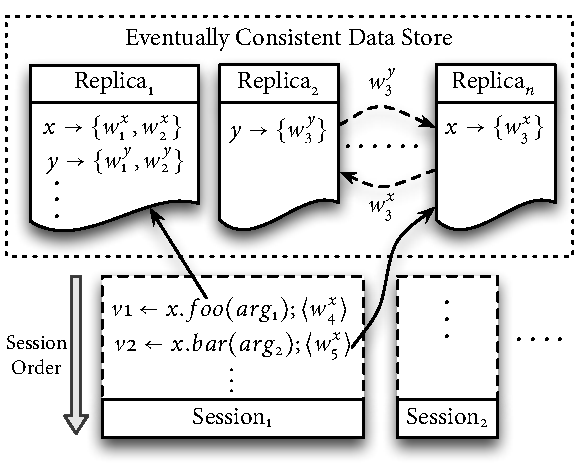
\includegraphics[width=0.65\columnwidth]{Figures/SystemModel}
\caption{\quelea system model.}
\label{fig:sysmod}
\end{figure}

Figure~\ref{fig:sysmod} provides a schematic diagram of our system model. The
distributed store is composed of a collection of \emph{replicas}, each of which
stores a set of \emph{objects} ($x,y,\ldots$). We assume that every object is
replicated at every replica in the store. The state of an object at any replica
is the set of all updates (\emph{effects}) performed on the object. For
example, the state of $x$ at replica 1 is the set composed of effects $w^x_1$
and $w^x_2$.

Each object is associated with a set of \emph{operations}. The clients interact
with the store by invoking operations on objects. The sequence of operations
invoked by a particular client on the store is called a \emph{session}. The
data store is typically accessed by a large number of clients (and hence
sessions) concurrently. Importantly, the clients are oblivious to which replica
an operation is applied to; the data store may choose to route the operation to
any replica in order to minimize latency, balance load, etc. For example, the
operations \emph{foo} and \emph{bar} invoked by the same session on the same
object, might end up being applied to different replicas because replica 1 (to
which \emph{foo} was applied) might be unreachable when the client invokes
\emph{bar}.

When \emph{foo} is invoked on a object $x$ with arguments \emph{arg}$_1$ at
replica 1, it simply \emph{reduces} over the current set of effects at that
replica on that object ($w^x_1$ and $w^x_2$), produces a result $v1$ that is
sent back to the client, and emits a \emph{single} new effect $w^x_4$ that is
appended to the state of $x$ at replica 1. Thus, every operation is evaluated
over a \emph{snapshot} of the state of the object on which it is invoked. In
this case, the effects $w^x_1$ and $w^x_2$ are \emph{visible} to $w^x_4$,
written logically as $\vis{w^x_1}{w^x_4} \wedge \vis{w^x_2}{w^x_4}$, where
$\visZ$ is the visibility relation between effects. Visibility is an
irreflexive and asymmetric relation, and only relates effects produced by
operations on the same object. Executing a read-only operation is similar
except that no new effects are produced.

The effect added to a particular replica is asynchronously sent to other
replicas, and eventually merged into all other replicas. Two effects $w^x_4$
and $w^x_5$ that arise from the same session are said to be in \emph{session
order} (written logically as $\so{w^x_4}{w^x_5}$). Session order is an
irreflexive, transitive relation. The effects $w^x_4$ and $w^x_5$ arising from
operations applied to the same object $x$ are said to be under the \emph{same
object} relation, written $\sameobj{w^x_4}{w^x_5}$. Finally, we can associate
every effect with the operation that generated the effect with the help of a
relation $\operZ$. In the current example, $\oper{w^x_4}{foo}$ and
$\oper{w^x_5}{bar}$ hold. For simplicity, we assume all operation names across
all object types are distinct.

This model admits all the inconsistencies associated with eventual consistency.
The goal of this work is to identify the precise consistency level for each
operation such that application-level constraints are not violated. In the next
section, we will concretely describe the challenges associated with
constructing a consistent bank account on top of an eventually consistent data
store. Subsequently, we will illustrate how our contract and specification
language, armed with the primitive relations $\visZ$, $\soZ$, $\sameobjZ$ and
$\operZ$, mitigates these challenges.

\section{Motivation}
\label{q_sec:motivation}

Consider how we might implement a highly available bank account on top of an
eventually consistent data store, with the \emph{integrity} constraint that the
balance must be non-negative. We begin by implementing a bank account
replicated data type (RDT) in \quelea, and then describe the mechanisms to
obtain the desired correctness guarantees.

\subsection{RDT Specification}

A key novelty in \quelea is that it allows the addition of new RDTs to the
store, which obviates the need for coercing the application logic to utilize
the store provided data types. In addition, \quelea treats the convergence
semantics of the data type separately from its consistency properties. This
separation of concerns permits \emph{operational} reasoning for conflict
resolution, and \emph{declarative} reasoning for consistency. The combination
of these techniques enhances the programmability of the store.

Let us assume that the bank account object provides three operations:
\cf{deposit}, \cf{withdraw} and \cf{getBalance}, with the assumption that the
withdraw fails if the account has insufficient balance. Every operation in
\quelea is of the following type, written in Haskell syntax:

\begin{codehaskell}
type Operation e a r = [e] -> a -> (r, Maybe e)
\end{codehaskell}

\noindent It takes a list of effects (the \emph{context} for the operation),
and an input argument, and returns a result along with an optional effect
(read-only operations return \cf{Nothing}). The new effect (if emitted) is
added to the state of the object at the current replica, and asynchronously
sent to other replicas. The implementation of the bank account operations in
\quelea is given in Figure~\ref{fig:ex}:

\begin{figure}
\begin{codehaskell}
data Acc = Deposit Int | Withdraw Int | GetBalance

getBalance :: [Acc] -> () -> (Int, Maybe Acc)
getBalance ctxt _ =
  let res = sum [x | Deposit x <- ctxt]
						- sum [x | Withdraw x <- ctxt]
	in (res, Nothing)

deposit :: [Acc] -> Int -> ((), Maybe Acc)
deposit _ amt = (amt, Just dollar Deposit amt)

withdraw :: [Acc] -> Int -> (Bool, Maybe Acc)
withdraw ctxt v =
	if sel1 dollar getBalance ctxt () >= v
  then (True, Just dollar Withdraw v)
	else (False, Nothing)
\end{codehaskell}
\caption{Definition of a bank account expressed in Quelea.}
\label{fig:ex}
\end{figure}

The datatype \cf{Acc} represents the effect type for the bank account. The
context of the operations is a snapshot of the state of the object at some
replica. In this sense, every operation on the RDT is atomic, and thus
permitting sequential reasoning for implementing eventually consistent data
types. We have implemented a large corpus of RDTs for realistic benchmarks
including shopping carts, auction and micro-blogging sites in few tens of lines
of code.

\subsection{Anomalies under Eventual Consistency}

Our goal is to choose the correct consistency level for each of the bank
account operations such that (1) the balance remains non-negative and (2) the
\cf{getBalance} operation never incorrectly returns a negative balance. Let us
first consider the anomalies that could arise under eventual consistency.

\begin{figure}
\centering
\subfigure[Unsafe withdraw]{\label{fig:unsafeWithdrawAnomaly}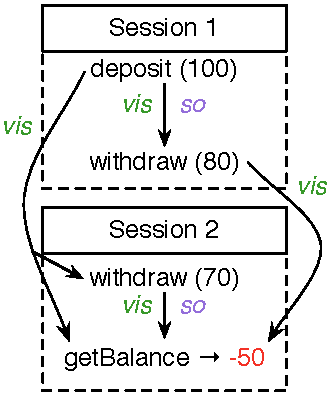
\includegraphics[width=0.34\columnwidth]{Figures/Motivation4}}
\hfill
\subfigure[Negative balance]{\label{fig:negativeBalanceAnomaly}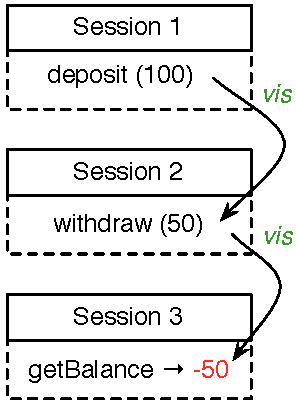
\includegraphics[width=0.31\columnwidth]{Figures/Motivation2}}
\hfill
\subfigure[Missing update]{\label{fig:missingUpdateAnomaly}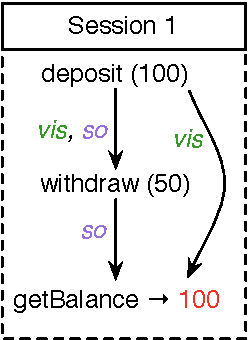
\includegraphics[width=0.26\columnwidth]{Figures/Motivation1}}
\caption{Anomalies possible under eventual consistency for the get balance operation.}
\label{fig:ba_anomalies}
\end{figure}

Consider the execution shown in Figure~\ref{fig:unsafeWithdrawAnomaly}. Assume
that all operations in the figure are on the same bank account object with the
initial balance being zero. Session 1 performs a \cf{deposit} of 100, followed
by a \cf{withdraw} of 80 in the same session. The \cf{withdraw} operation
witnesses the deposit and succeeds\footnote{Although visibility and session
order relations relate effects, we have abused the notation in these examples
to relate operations, with the idea that the relations relate the effect
emitted by those operations}. Subsequently, session 2 perform a \cf{withdraw}
operation, but importantly, due to eventual consistency, only witnesses the
\cf{deposit} from session 1, but not the subsequent withdraw. Hence, this
\cf{withdraw} also \emph{incorrectly} succeeds, violating the integrity
constraint. A subsequent \cf{getBalance} operation, that happens to witness all
the previous operations, would report a negative balance.

It is easy to see that preventing concurrent \cf{withdraw} operations
eliminates this anamoly. This can be done by insisting that \cf{withdraw} be
executed as a strongly consistent operation. Despite this strengthening,
\cf{getBalance} operation may incorrectly report a negative balance to the end
user. Consider the execution shown in fig.~\ref{fig:negativeBalanceAnomaly},
which consists of three concurrent sessions performing a \cf{deposit}, a
\cf{withdraw}, and a \cf{getBalance} operation, respectively, on the same bank
account object. As the \cf{vis} edge indicates, operation \cf{withdraw(50)} in
session 2, witnesses the effects of \cf{deposit(100)} from session 1, concludes
that there is sufficient balance, and completes successfully. However, the
\cf{getBalance} operation may only witness this successful withdraw, but not
the causally preceding \cf{dopsit}, and reports the balance of negative 50 to
the user.

Under eventual consistency, the users may also be exposed to other forms of
inconsistencies. Figure~\ref{fig:missingUpdateAnomaly} shows an execution where
the \cf{getBalance} operation in a session does not witness the effects of an
earlier \cf{withdraw} operation performed in the same session, possibly because
it was served by a replica that has not yet merged the \cf{withdraw} effect.
This anomaly leads the user to incorrectly conclude that the \cf{withdraw}
operation failed to go through.

Although it is easy to understand the reasons behind the occurrence of the
aforementioned anomalies, finding the appropriate fixes is not readily
apparent. Making \cf{getBalance} a strongly consistent operation is definitely
sufficient to avert anomalies, but is it really necessary? Given the cost of
enforcing strong consistency~\cite{DynamoDB,Terry2013}, it is preferable to avoid
it unless there are no viable alternatives. Exploring the space of these
alternatives requires understanding the subtle differences in semantics of
various kinds of weak consistency alternatives.

\subsection{Contracts}

\quelea helps facilitate the mapping of operations to appropriate consistency
levels by letting the programmer declare application-level consistency
constraints as \emph{contracts}
(Figure~\ref{fig:contract-lang}\footnote{\quelea exposes the contract
construction language as a Haskell library}) that axiomatically specify the set
of allowed executions involving this operation. In the case of the bank
account, any execution that does not exhibit the anomalies described in the
previous section is a \emph{well-formed} execution on the bank account object.
By specifying the set of legal executions for each data type in terms of a
trace of operation invocations on that type, \quelea\ ensures that all
executions over that type are well-formed.

In our running example, it is clear that in order to preserve the integrity
constraint, the \cf{withdraw} operation must be strongly consistent.  That is,
given two \cf{withdraw} operations $a$ and $b$, either $a$ is visible to $b$ or
vice versa. We express this application-level consistency requirement as a
contract ($\cv_w$) over \cf{withdraw}:
\begin{mathpar}
\begin{array}{l}
\forall (a : \rcf{withdraw}).~\sameobj{a}{\cureff} \Rightarrow a = \cureff \vee \vis{a}{\cureff} \vee \vis{\cureff}{a}
\end{array}
\end{mathpar}

\noindent Here, $\cureff$ stands for the effect emitted by the \cf{withdraw} operation.
The syntax $a:\rcf{withdraw}$ states that $a$ is an effect  emitted
by a \cf{withdraw} operation i.e., $\oper{a}{\rcf{withdraw}}$ holds.  The
contract specifies that if the current operation emits an effect $\cureff$,
then for any operation $a$ which was emitted by a \cf{withdraw} operation, it
is the case that $a = \cureff$ or $a$ is visible to $\cureff$, or vice versa.
Any execution on a bank account object that preserves the above contract for a
\cf{withdraw} operation is said to be derived from a correct implementation of
\cf{withdraw}.

\noindent For \cf{getBalance}, we construct the following contract ($\cv_{gb}$):
\begin{mathpar}
\begin{array}{l}
\forall (a:\rcf{deposit}), (b:\rcf{withdraw}), (c: \rcf{deposit} \vee \rcf{withdraw}). \\
\qquad \vis{a}{b} \wedge \vis{b}{\cureff} \Rightarrow \vis{a}{\cureff} \\
\qquad \wedge~ (\soZ \cap \sameobjZ) (c,\cureff) \Rightarrow \vis{c}{\cureff}
\end{array}
\end{mathpar}

\noindent The expression $c:\rcf{deposit} \vee \rcf{withdraw}$ states that $c$
is an effect that was emitted either by a \cf{deposit} or a \cf{withdraw}
operation. If a \cf{withdraw} $b$ is visible to \cf{getBalance} $\cureff$, then
all \cf{deposit} operations $a$ visible to $b$ should also be visible to
$\cureff$. This prevents negative balance anomalies. Our contract language
provides operators to compose relations. The syntax $(R_1 \cap R_2)(a,b)$ is
equivalent to $R_1(a,b) \wedge R_2(a,b)$. The last line of the above contract
says that if a \cf{deposit} or a \cf{withdraw} operation precedes a
\cf{getBalance} operation in session order, and is applied on the same object
as the \cf{getBalance} operation, then it must be the case that the
\cf{getBalance} operation witnesses the effects of the preceding operations.

Finally, since there are no restrictions on when or how a \cf{deposit}
operation can execute, its contract is simply $\small \true$.

\subsection{From Contracts to Implementation}

Notice that the contracts for \cf{withdraw} and \cf{getBalance} only express
application-level consistency requirements, and make no reference to the
semantics of the underlying store. To write contracts, a programmer only needs
to reason about the semantics of the application under the \quelea system model.
The mapping of application-level consistency requirements to appropriate
store-level guarantees is done automatically behind-the-scene. How might one go
about ensuring that an execution adheres to a contract? The challenge is that a
contract provides a declarative (axiomatic) specification of an execution,
while what is required is an operational procedure for \emph{enforcing} its
implicit constraints.

One strategy would be to execute operations speculatively.  Here, operations
are tentatively applied as they are received from the client or other replicas.
We can maintain a runtime manifestation of executions, and check
well-formedness conditions at runtime, rolling back executions if they are
ill-formed. However, the overhead of state maintenance and the complexity of
user-defined contracts is likely to make this technique infeasible in practice.

We devise a static approach instead. Contracts are analyzed with the help of a
theorem prover, and statically mapped to a particular store-level consistency
property that the prover guarantees preserves contract semantics. We call this
procedure \emph{contract classification}. Given the variety and complexity of
store level consistency properties, the idea is that the system implementor
parameterizes the classification procedure by describing the store semantics in
the \emph{same} contract language as the one used to express the contract on
the operations. In the next section, we describe the contract language in
detail and describe the classification procedure for a particular store
semantics.

\section{Contract Language}
\label{q_sec:lang}

\begin{figure}[t]
\begin{mathpar}
\begin{array}{rclcl}
\multicolumn{5}{c}{
  {x,y,\cureff} \in \mathtt{EffVar} \qquad \qquad
  {\sf Op} \in \mathtt{OperName}
}\\
\cv 		& \in & \mathtt{Contract} 	& \coloneqq & \forall (x : \tau).\cv
        \ALT \pi \\
\tau		& \in	& \mathtt{EffType}	& \coloneqq &  {\sf Op}
        \ALT \tau \vee \tau \\
\pi			&	\in & \mathtt{Prop} & \coloneqq & \true \ALT R(x,y)
        \ALT \pi \vee \pi \\
			  & 		&	 &  \ALT & \pi \wedge \pi \ALT \pi \Rightarrow \pi \\
R				& \in & \mathtt{Relation}	& \coloneqq & \visZ \ALT \soZ
        \ALT \sameobjZ \ALT R^+ \\
				&			&	 &  \ALT & R \cup R \ALT R \cap R \\
\end{array}
\end{mathpar}
\caption{Contract language.}
\label{fig:contract-lang}
\end{figure}

\subsection{Syntax}

The syntax of our core contract language is shown in Figure
~\ref{fig:contract-lang}. The language is based on first-order logic (FOL), and
admits prenex universal quantification over typed and untyped effect variables.
We use a special effect variable ($\cureff$) to denote the effect of
\emph{current operation} - the operation for which a contract is being written.
The type of an effect is simply the name of the operation (eg: \cf{withdraw})
that induced the effect. We admit disjunction in types to let an effect variable
range over multiple operation names. The contract $\small \forall (a : \tau_1
\vee \tau_2).~\psi$ is just syntactic sugar for $\small \forall a.
(\oper{a}{\tau_1} \vee \oper{a}{\tau_2}) \Rightarrow \psi$. An untyped effect
variable ranges over all operation names.

Quantifier-free propositions in our contract language are conjunctions,
disjunctions and implications of predicates expressing relations between pairs
of effect variables. The syntactic class of relations is seeded with primitive
$\visZ$, $\soZ$, and $\sameobjZ$ relations, and also admits derived relations
that are expressible as union, intersection, or transitive
closure\footnote{Strictly speaking, $R^{+}$ is not the transitive closure of
$R$, as transitive closure is not expressible in FOL.  Instead, $R^{+}$ in our
language denotes \emph{a} superset of transitive closure of $R$. Formally,
$R^{+}$ is any relation $R'$ such that forall $x$, $y$, and $z$, a) $R(x,y)
\Rightarrow R'(x,y)$, and b) $R'(x,y) \conj R'(y,z) \Rightarrow R'(x,z)$} of
primitive relations.

\begin{itemize}

\item Same object session order: $\sooZ = \soZ ~\cap~ \sameobjZ$.

\item Happens-before order: $\hbZ = (\soZ ~\cup~ \visZ)^+$.

\item Same object happens-before order: $\hboZ = (\sooZ ~\cup~ \visZ)^+$.

\end{itemize}

\subsection{Semantics}

\begin{figure}[t]
\begin{mathpar}
\begin{array}{lclcl}
\multicolumn{5}{l}{
  {\eff} \in \mathtt{Effect} \qquad
  {\cv} \in \mathtt{Contract} \qquad
  \set{\eff} \in \mathtt{Effect\; Set}
}\\
\EffSoup & \in & \mathtt{EffSoup}	  & \coloneqq & \set{\eff} \\
\visZ, \soZ, \sameobjZ &	\in & \mathtt{Relations} & \coloneqq & \EffSoup \times \EffSoup \\
%\sameobjZ		&     &  & \\
{\E} 		& \in & \mathtt{ExecState}  & \coloneqq & \Exec \\
\end{array}
\end{mathpar}

\caption{Axiomatic execution.}
\label{sem:ax_ex}
\end{figure}

\quelea contracts are constraints over axiomatic definitions of program
executions. Figure~\ref{sem:ax_ex} summarizes artifacts relevant to define
an axiomatic execution. We formalize an axiomatic execution as a tuple $\Exec$,
where $\EffSoup$, called the \emph{effect soup}, is the set of all effects
generated during the program execution, and $\visZ,\soZ,\sameobjZ \subseteq
\EffSoup \times \EffSoup$ are \emph{visibility}, \emph{session order}, and
\emph{same object} relations, respectively, witnessed over generated effects at
run-time.

Note that the axiomatic definition of an execution ($\E$) provides
interpretations for primitive relations (eg: $\visZ$) that occur free in
contract formulas, and also fixes the domain of quantification to set of all
effects ($\EffSoup$) observed during the program execution. As such, $\E$ is a
potential model for any first-order formula ($\cv$) expressible in our contract
language. If $\E$ is indeed a valid model for $\cv$ (expressed using the
model-theoretic consequence relation as $\E \models \cv$), we say that the
execution $\E$ satisfied the contract $\cv$:

\begin{definition}
An axiomatic execution $\E$ is said to satisfy a contract $\cv$ if and only if
$\E \models \cv$.
\end{definition}

\subsection{Capturing Store Semantics}
\label{q_sec:store_sem}

An important aspect of our contract language is its ability to capture
store-level consistency guarantees, along with application-level consistency
requirements. Similar to~\cite{Burckhardt2014}, we can rigorously define a wide
variety of store semantics including those that combine any subset of session
and causality guarantees, and multiple consistency levels.  However, for our
purposes, we identify three particular consistency levels -- eventual, causal,
and strong, commonly offered by many distributed stores with tunable
consistency, with increasing overhead in terms of latency and availability.

\begin{itemize}
\setlength{\itemsep}{2pt}

\item \textbf{Eventually consistency}: Eventually consistent operations can
	be satisfied as long as the client can reach at least one replica. In the
	bank account example, \cf{deposit} is an eventually consistent operation.
	While eventually consistent data stores typically offer \emph{basic} eventual
	consistency with all possible anomalies, we assume that our store provides
	stronger semantics that remain highly-available~\cite{BailisHAT,COPS}; the
	store always exposes a \emph{causal cut} of the updates. This semantics can
	be formally captured in terms of the following contract definition:
  \begin{mathpar}
  \ecc = \forall a,b. ~\hbo{a}{b} \wedge \vis{b}{\cureff} \Rightarrow \vis{a}{\cureff}
  \end{mathpar}

\item \textbf{Causal consistency}: Causally consistent operations are required
	to see a causally consistent snapshot of the object state, including the
	actions performed on the same session.  The latter requirement implies that
	if two operations $o_1$ and $o_2$ from the same session are applied to two
	different replicas $r_1$ and $r_2$, the second operation cannot be discharged
	until the effect of $o_1$ is included in $r_2$. The \cf{getBalance} operation
	requires causal consistency, as it requires the operations from the same
	session to be visible, which cannot be guaranteed under eventual consistency.
	The corresponding store semantics is captured by the contract $\ccc$ defined
	below:
  \begin{mathpar}
  \ccc = \forall a.~\hbo{a}{\cureff} \Rightarrow \vis{a}{\cureff}
  \end{mathpar}

\item \textbf{Strong Consistency}: Strongly consistent operations may block
  indefinitely under network partitions. An example is the total-order
  contract on \cf{withdraw} operation. The corresponding store semantics is
	captured by the $\scc$ contract definition:
  \begin{mathpar}
  \scc = \forall a.~\sameobj{a}{\cureff} \Rightarrow \vis{a}{\cureff} ~\vee~ \vis{\cureff}{a} ~\vee~ a = \cureff
  \end{mathpar}

\end{itemize}

\newcommand{\DDe}[1]{#1}
\begin{figure}[t]
\begin{mathpar}
\begin{array}{c}
\RuleTwo
{\DDe{\cv} \le \DDe{\scc}}
{{\sf WellFormed}(\cv)}  \qquad

\RuleTwo
{\DDe{\cv} \le \DDe{\ecc}}
{{\sf EventuallyConsistent}(\cv)} \\ \\

\RuleTwo
{\DDe{\cv} \not\le \DDe{\ecc}
\quad \DDe{\cv} \le \DDe{\ccc}}
{{\sf CausallyConsistent}(\cv)} \qquad

\RuleTwo
{\DDe{\cv} \not\le \DDe{\ccc}
\quad \DDe{\cv} \le \DDe{\scc}}
{{\sf StronglyConsistent}(\cv)}

\end{array}
\end{mathpar}
\caption{Contract classification.}
\label{sem:classify}
\end{figure}

\subsection{Contract Comparison and Classification}

Our goal is to map application-level consistency constraints on operations to
appropriate store-level consistency guarantees capable of satisfying these
constraints.  The ability to express both these kinds of constraints as
contracts in our contract language lets us compare and determine if contract
($\cv_{op}$) of an operation ($\mathit{op}$) is weak enough to be satisfied
under a store consistency level identified by the contract $\cv_{st}$. Towards
this end, we define a binary \emph{weaker than} relation for our contract
language as following:

\begin{definition}
A contract $\cv_{op}$ is said to be weaker than $\cv_{st}$ (written $\cv_{op}
\le \cv_{st}$ ) if and only if $\Delta \vdash \forall \cureff.
\cv_{st} \Rightarrow \cv_{op}$.
\end{definition}

The quantifier in the sequent binds $\cureff$ that occurs free in $\cv_{st}$ and
$\cv_{op}$. Context ($\Delta$) of the sequent is a conjunction of assumptions
about the nature of primitive relations. A \emph{well-formed} axiomatic
execution ($\E$) is expected to satisfy these assumptions (i.e., $\E \models
\Delta$).

\begin{definition}
An axiomatic executions $\E = \Exec$ is said to be well-formed if the following
axioms ($\Delta$) hold:

\begin{itemize}
\item The happens-before relation is acyclic: $\forall a.~\neg\hb{a}{a}$.
\item Visibility only relates actions on the same object: $\forall a,b.~\vis{a}{b} \Rightarrow \sameobj{a}{b}$.
\item Session order is a transitive relation: $\forall a,b,c.~\so{a}{b} ~\wedge~ \so{b}{c} \Rightarrow \so{a}{c}$.
\item Same object is an equivalence relation:
	\begin{itemize}
	\item $\forall a.~\sameobj{a}{a}$.
	\item $\forall a,b.~\sameobj{a}{b} \Rightarrow \sameobj{b}{a}$.
	\item $\forall a,b,c.~\sameobj{a}{b} ~\wedge~ \sameobj{b}{c} \Rightarrow \sameobj{a}{c}$.
	\end{itemize}
\end{itemize}
\end{definition}

If the contract ($\cv_{op}$) of an operation ($\mathit{op}$) is \emph{weaker
than} a store contract ($\cv_{st}$), then constraints expressed by the former
are implied by guarantees provided by the latter. The completeness of
first-order logic allows us to assert that any well-formed execution ($\E$)
that satisfies $\cv_{st}$ (i.e., $\E\models \cv_{st}$) also satisfies
$\cv_{op}$ (i.e., $\E \models \cv_{op}$). Consequently, it is safe to execute
operation $\mathit{op}$ under a store consistency level captured by $\cv_{st}$.

Observe that the contracts $\scc$, $\ccc$ and $\ecc$ are themselves totally
ordered with respect to the $\le$ relation: $\ecc \le \ccc \le \scc$.  This
concurs with the intuition that any contract satisfiable under $\ecc$ or $\ccc$
is satisfiable under $\scc$, and any contract that is satisfiable under $\ecc$
is satisfiable under $\ccc$. We are interested in the \emph{weakest} guarantee
(among $\ecc$, $\ccc$, and $\scc$) required to satisfy the contract. We define
the corresponding consistency level as the \emph{consistency class} of the
contract.

The classification scheme, presented formally in Figure~\ref{sem:classify},
defines rules to judge the consistency class of a contact. For example, the
scheme classifies the \cf{getBalance} contract ($\cv_{gb}$) from
Section~\ref{q_sec:motivation} as a {\sf\small CausallyConsistent} contract, because
the sequent $\Delta \vdash \ccc \Rightarrow \cv_{gb}$ is valid in first-order
logic (therefore, $\cv_{gb} \le \ccc$), whereas the sequent $\Delta \vdash \ecc
\Rightarrow \cv_{gb}$ is invalid (therefore, $\cv_{gb} \not\le \ecc$). Since we
confine of our contract language to a decidable subset of the logic, validity
of such sequents can be decided mechanically allowing us to automate the
classification scheme in \quelea.

Along with three straightforward rules that classify contracts into consistency
classes, the classification scheme also presents a rule that judges
well-formedness of a contract. A contract is well-formed if and only if it is
satisfiable under $\scc$ - the strongest possible consistency guarantee that
the store can provide. Otherwise, it is considered ill-formed, and rejected
statically.

\subsection{Soundness of Contract Classification}

We now present a meta-theoretic result that certifies the soundness of
classification-based contract enforcement. To help us state the result, we
define an operational semantics of the our system described informally in
Section~\ref{q_sec:sysmod}:
\begin{mathpar}
\begin{array}{lclcl}
{\it op} 	& \in & \mathtt{Operation} \\
{\tau}		& \in & \mathtt{Consistency Class} 	& \coloneqq & {\sf ec},{\sf cc},{\sf sc} \\
{\sigma} 	& \in & \mathtt{Session} 					 	& \coloneqq & \cdot \ALT \langle op,\tau \rangle; \sigma \\
\Sigma 		& \in & \mathtt{Session\;Soup}   	 	& \coloneqq & \sigma \pll \Sigma \ALT \emptyset \\
					&			&	\mathtt{Config}		  			 	& \coloneqq & \E,\Sigma \\
\end{array}
\end{mathpar}

We model the system as a tuple $\E,\Sigma$, where the axiomatic execution $\E$
captures the data store's current state, and session soup $\Sigma$ is the set
of concurrent client sessions interacting with the store. A session $\sigma$ is
a sequence of pairs composed of replicated data type operations $\mathit{op}$,
tagged with the consistency class $\tau$ of their contracts (as determined by
the contract classification scheme). We assume a reduction relation of form:
\begin{mathpar}
  \auxred{} {\E,\langle op,\tau \rangle;\sigma \pll \Sigma} {\eff}
    {\E',\sigma \pll \Sigma}
\end{mathpar}

\noindent on the system state. The relation captures the progress of the
execution (from $\E$ to $\E'$)  due to the successful completion of a client
operation $\mathit{op}$ from one of the sessions in $\Sigma$, generating a new
effect $\eff$. If the resultant execution $\E'$ satisfies the store contract
$\cv_\tau$ (i.e., $\E \models \cv_\tau$), then we say that the store has
\emph{enforced} the contract $\cv_\tau$ in the execution $\E'$. With help of
the operational semantics, we now state the soundness of contract enforcement
as follows:

\begin{theorem}[Soundness of Contract Enforcement]
\label{thm:classification-sound}
Let $\cv$ be a well-formed contract of a replicated data type operation
$\mathit{op}$, and let $\tau$ denote the consistency class of $\cv$ as
determined by the contract classification scheme. For all well-formed execution
states $\E$, $\E'$ such that
$\auxred{} {\E,\langle op,\tau \rangle;\sigma \pll \Sigma} {\eff} {\E', \sigma
\pll \Sigma}$, if $\E' \models \cv_\tau[\eff/\cureff]$, then $\E' \models
\cv[\eff/\cureff]$
\end{theorem}

The theorem states that if a data store correctly enforces $\scc$, $\ccc$, and
$\ecc$ contracts in all well-formed executions, then the same store, extended
with the classification scheme shown in Figure~\ref{sem:classify}, can enforce
all well-formed \quelea contracts. The proof of the theorem is given below:

\begin{proof}
  Hypothesis:
  \begin{mathpar}
  \begin{array}{cr}
    \auxred{} {\E,\langle op,\tau \rangle;\sigma \pll \Sigma} {\eff}
    {\E', \sigma \pll \Sigma} & H\npp\\
    \E' \models \cv_\tau[\eff/\cureff] & H\npp\\
  \end{array}
  \end{mathpar}
  Since $\tau$ is the contract class of $\cv$, by inversion, we have
  $\cv \le \cv_\tau$. By the definition of $\le$ relation:
  \begin{mathpar}
  \begin{array}{cr}
    \Delta \vdash \forall \cureff. \cv_\tau \Rightarrow \cv & H\npp\\
  \end{array}
  \end{mathpar}
   Since $\eff$ denotes new effect, it is a fresh variable that does
   not occur free in $\Delta$. From $H3$, after instantiating bound
   $\cureff$ with $\eff$, we have:
  \begin{mathpar}
  \begin{array}{cr}
    \Delta \vdash \cv_\tau[\eff/\cureff] \Rightarrow \cv[\eff/\cureff]
      & H\npp\\
  \end{array}
  \end{mathpar}
  Due to the soundness of natural deduction for first-order logic,
  $H4$ implies that for all models $\mathcal{M}$ such that
  $\mathcal{M} \models \Delta$, if $\mathcal{M} \models
  \cv_\tau[\eff/\cureff]$ then $\mathcal{M} \models
  \cv[\eff/\cureff]$. Since $\E'$ is well-formed, we have:
  \begin{mathpar}
  \begin{array}{cr}
    \E' \models \Delta & H\npp\\
  \end{array}
  \end{mathpar}
  Proof follows from $H1$, $H5$, and $H4$.
  \hfill \qed
\end{proof}

It is important to note that Theorem~\ref{thm:classification-sound} does not
ascribe any semantics to the reduction relation ($\xrightarrow{}$). As such, it
makes no assumptions about how the store actually implements ${\sf ec}$, ${\sf
cc}$ and ${\sf sc}$ guarantees. The specific implementation strategy is
determined by the operational semantics of the store, which \emph{defines} the
reduction relation for that particular store. The following section describes
operational semantics of the store used by the \quelea implementation.

\section{Operational Semantics}
\label{q_sec:meta-theory}

\renewcommand{\auxred}[4]{#1 \vdash #2 \;\xhookrightarrow{#3}\; #4 }

We now describe operational semantics of a data store that implements
strong, causal and eventual consistency guarantees. The semantics also
serves as a high-level description of our implementation of the store
underlying \quelea.

\begin{figure*}
\textbf{RDT Specification Language}\\
\begin{minipage}{\columnwidth}
\begin{mathpar}
\stretcharraybig
\begin{array}{lclcl}
{\delta} & \in & \mathtt{Replicated Datatype}& &\\
{v} & \in & \mathtt{Value} & & \\
{e} & \in & \mathtt{Expression} & &\\
{op} & \in & \mathtt{Operation}& & \\
\Ops & \in & \mathtt{Operation Definition}   & \coloneqq & op \mapsto e \\
\cv & \in & {\sf Contract} & &\\
\Ctrts & \in & \mathtt{Operation Contract} & \coloneqq & op \mapsto \cv \\
   &   & \mathtt{RDT Specification} & \coloneqq & (\delta,\Ops,\Ctrts)
\end{array}
\end{mathpar}
\end{minipage}

\begin{minipage}{\columnwidth}
\textbf{System Model}\\
\begin{mathpar}
\stretcharraybig
\begin{array}{lclcl}
\multicolumn{5}{c}{
{s} \in \SessID \qquad
{i} \in \EffID \qquad
{r} \in \ReplID } \\
\eff & \in & \mathtt{Effect} & \coloneqq &  (s,~i,~op,~v)\\
\EffSoup & \in & \mathtt{EffSoup}	  & \coloneqq & \set{\eff} \\
\visZ, \soZ, \sameobjZ &	\in & \mathtt{Relations} & \coloneqq & \EffSoup \times \EffSoup \\
{\E} 		& \in & \mathtt{ExecState}  & \coloneqq & \Exec \\
\Theta  & \in & \mathtt{Store}      & \coloneqq & r \mapsto \set{\eff} \\
{\tau}		& \in & \mathtt{Consistency Class} 	& \coloneqq & {\sf ec},{\sf cc},{\sf sc} \\
{\sigma} 	& \in & \mathtt{Session} 					 	& \coloneqq & \cdot \ALT op_\tau::\sigma \\
\Sigma 		& \in & \mathtt{Session\;Soup}   	 	& \coloneqq &
      \langle s, i, \sigma \rangle \pll \Sigma \ALT \emptyset \\
					&			&	\mathtt{Config}		  			 	& \coloneqq & (\E, \Theta, \Sigma)
\end{array}
\end{mathpar}
\end{minipage}

\textbf{Auxiliary Definitions}\\
\begin{minipage}{\columnwidth}
\begin{mathpar}
\stretcharraybig
\begin{array}{lcl}
\operZ(s,~i,~op,~v) & = & op \\
\ctxtFn(s,~i,~op,~v) & = & (op,~v) \\
\end{array}
\end{mathpar}
\end{minipage}
\caption{Syntax and states of operational semantics.}
\label{sem:oper-syn}
\end{figure*}


\begin{figure*}
\textbf{Auxiliary Reductions} \;
  \fbox{\(\auxred{\Theta} {(\E,\langle s,i,op \rangle)} {r} {(\E',\eff)}\)}\\

\begin{minipage}{\textwidth}
\rulelabel{Oper}
\begin{mathpar}
\stretcharraybig
\begin{array}{l}
\RuleTwo
{
r \in \dom(\Theta) \qquad
ctxt = {\ctxtFn}^{*}(\Theta(r)) \qquad
\Ops(op)(ctxt) {\rdtredsto}^{*} v \\
\eff = (s,i,op,v) \qquad
\{\eff'\} = \EffSoup_{({\sf SessID}=s,\,{\sf SeqNo}=i-1)}\\
\EffSoup' = \{\eff\} \cup \EffSoup \qquad
\visZ' = \Theta(r)\times\{\eff\} \cup \visZ \\
\soZ' = (\soZ^{-1}(\eff') \cup \eff') \times\{\eff\} \cup \soZ
\qquad
\sameobjZ' = \EffSoup' \times \EffSoup'
}
{
  \auxred {\Theta} {((\EffSoup,\visZ,\soZ,\sameobjZ), \langle s,i,op \rangle}
  {r} {((\EffSoup',\visZ',\soZ',\sameobjZ'),\eff)}
}
\end{array}
\end{mathpar}
\end{minipage}


\vspace{5mm}
\textbf{Operational Semantics} \;
  \fbox{\((\E,\Theta,\Sigma) \;\xrightarrow{\eff}\; (\E',\Theta',\Sigma')\)}\\

\begin{minipage}{\columnwidth}
\rulelabel{EffVis}
\begin{mathpar}
\stretcharraybig
\begin{array}{l}
\RuleTwo
{
  \eff \in \EffSoup \quad
  \Theta' = \Theta \cup [r \mapsto \{\eff\} \cup \Theta(r)]\\
  \eff \notin \Theta(r) \qquad
  \E.\visZ^{-1}(\eff) \cup \E.\soZ^{-1}(\eff) \subseteq \Theta(r)\\
}
{
  (\E,\Theta,\Sigma) \;\xrightarrow{\eff}\; (\E, \Theta', \Sigma)
}
\end{array}
\end{mathpar}
\end{minipage}
\begin{minipage}{\columnwidth}
\rulelabel{EC}
\begin{mathpar}
\stretcharraybig
\begin{array}{l}
\RuleTwo
{
  \tau = {\sf EventuallyConsistent} \qquad
  \auxred{\Theta} {(\E,\langle s,i,op \rangle)} {r} {(\E',\eff)}
}
{
  (\E,\Theta,\langle s,i,op_\tau::\sigma \rangle \pll \Sigma)
    \;\xrightarrow{\eff}\;
  (\E',\Theta, \langle s,i+1,\sigma \rangle\pll \Sigma)
}
\end{array}
\end{mathpar}
\end{minipage}
\begin{minipage}{\columnwidth}
\rulelabel{CC}
\begin{mathpar}
\stretcharraybig
\begin{array}{l}
\RuleTwo
{
  \tau = {\sf CausallyConsistent} \qquad
  \auxred{\Theta} {(\E,\langle s,i,op \rangle)} {r} {(\E',\eff)} \qquad
  \E'.\soZ^{-1}(\eff) \subseteq \Theta(r)
}
{
  (\E,\Theta,\langle s,i,op_\tau::\sigma \rangle \pll \Sigma)
    \;\xrightarrow{\eff}\;
  (\E',\Theta,\langle s,i+1,\sigma \rangle \pll \Sigma)
}
\end{array}
\end{mathpar}
\end{minipage}
\begin{minipage}{\columnwidth}
\rulelabel{SC}
\begin{mathpar}
\stretcharraybig
\begin{array}{l}
\RuleTwo
{
  \tau = {\sf StronglyConsistent} \qquad
  \auxred{\Theta} {(\E,\langle s,i,op \rangle)} {r}
  {(\E',\eff)} \qquad \E.A \subseteq \Theta(r) \\
  \dom(\Theta') = \dom(\Theta) \qquad
  \forall r'\in \dom(\Theta'). \Theta'(r') = \Theta(r') \cup \{\eff\}
}
{
  (\E, \Theta, \langle s,i,op_\tau::\sigma \rangle \pll \Sigma)
    \;\xrightarrow{\eff}\;
  (\E, \Theta', \langle s,i+1,\sigma \rangle \pll \Sigma)
}
\end{array}
\end{mathpar}
\end{minipage}

\caption{Operational semantics of a replicated data store.}
\label{sem:oper}
\end{figure*}


Figures~\ref{sem:oper-syn} and \ref{sem:oper} present operational semantics as
rules defining the reduction relation ($\xrightarrow{}$) over the execution
state.  Since we now have a concrete store, we extend our system model with
$\Theta$, a representation of the store as a map from replicas to their local
states. The local state of a replica $r$ (i.e., $\Theta(r)$) is a set of
effects that are currently visible at $r$. An operation $op$ performed at
replica $r$ can only witness the set of effects ($\Theta(r)$) visible at $r$.
To avoid too many paranthesis in our formal presentation, we represent
operation $op$, whose contract is in consistency class $\tau$, as $op_\tau$
instead of the usual $\langle op,\tau \rangle$. For the sake of clarity, we
only consider a single replicated object of well-defined type (for eg: a
replicated object of type \cf{BankAccount}) in our formalization.  Our
semantics are parametric over the specification of this replicated data type.
Figure~\ref{sem:oper} formalizes replicated data type (RDT) specification as
tuple $(\delta,\Ops,\Ctrts)$, where $\delta$ is the data type, $\Ops$ maps
labels ($op$) of operations on $\delta$ to their definitions, while $\Ctrts$
maps them to their consistency contracts ($\cv$). The definition of an
operation is expected to be a lambda expression, although we do not enforce
this in our formalization. For technical reasons, we tag each session with a
session identifier ($s$) and the sequence number ($i$) of the next operation in
the session.

The state of an operational execution ($\E$) is a tuple $\Exec$ where
$\EffSoup$ is a set of effects, and $\visZ$, $\soZ$, $\sameobjZ$ $\subseteq$
$\EffSoup \times \EffSoup$ are \emph{visibility}, \emph{session order}, and
\emph{same object} relations over effects, respectively. We define an effect
($\eff$) as a tuple $(s,i,op,v)$, which records the fact that $i^{th}$ action
in session with {\sf SessID} $s$, which is an operation $op$ on the replicated
object, has been successfully executed on some replica yielding a return value
$v$. Note that the combination of $s$ and $i$ uniquely identifies the effect.
Session order relation ($\soZ$) relates effects generated by the same session.
An effect $\eff = (s,i,op,v)$ is said to precede another effect $\eff' =
(s',i',op',v')$ in session order if and only if $s'=s$ and $i'\ge i$. Since we
only consider one replicated object in our formalization, the $\sameobjZ$
relation relates every pair of effects in the effect soup ($\EffSoup$). An
effect generated at a replica becomes visible at rest of the replicas
eventually.  If we denote the effect generated by the operation $op$ as
$\eff_{op}$, then $\Theta(r) \times \{\eff_{op}\} ~\subseteq~ \visZ$. Often, in
our formalization, we use $\visZ$ and $\soZ$ binary relations to obtain a set
of effects visible to a given effect $\eff$, or set of effects that precede a
given effect $\eff$ in the session order. As a syntactic convenience, whenever
$R$ is a binary relation, we write $R(\eff)$ to denote the set of all $\eff'$
such that $(\eff,\eff') \in R$.  Conversely, we write $R^{-1}(\eff)$ to denote
the set of all $\eff'$ such that $(\eff',\eff) \in R$.

Basic gurantee provided by the store is causal visibility, which is captured by
the rule $\rulelabel{EffVis}$ as a condition for an effect to be visible at a
replica. The rule makes an effect ($\eff$) visible at a replica $r$ only after
all the effects that causally precede $\eff$ are made visible at $r$.  It is
important to note that that enforcing causal visibility does not require any
inter-replica coordination. Any eventually consistent store can provide causal
visibility while being eventually consistent.  Therefore, we do not lose any
generality by assuming that the store provides causal visiblity.

Rule $\rulelabel{Oper}$ is an auxiliary reduction of the
\begin{mathpar}
\auxred{\Theta} {(\E,\langle s,i,op \rangle)} {r} {(\E',\eff)}
\end{mathpar}

\noindent Under the store configuration $\Theta$, the rule captures
the progress in execution (from $\E$ to $\E'$) due to the application
of operation $op$ to replica $r$ resulting in a new effect $\eff$.
The rule first constructs a \emph{context} for the application from
the local state ($\Theta(r)$) of the replica, by
projecting\footnote{{\textsf{ctxt*}} is auxiliary function
\textsf{ctxt} extended straightforwardly to set of effects} relevant
information from effects in $\Theta(r)$. It then substitutes the
definition ($\Ops(op)$) of the operation for its label ($op$), and
relies on the reduction relation ($\rdtredsto$) of the server-side
language to reduce the application $\Ops(op)(ctxt)$ to a value $v'$.
Subsequently, the the attributes of execution state, namely
$\EffSoup$, $\visZ$, $\soZ$, and $\sameobjZ$ are extended to
incorporate the new effect ($\eff$).

If the operation $op$ is {\sf EventuallyConsistent}, we simply apply
the operation to any replica $r$. Since the store provides causal
visibility, eventually consistent operations are satisfiable under any
replica. If the operation is {\sf CausallyConsistent}, the operation
can be applied to a replica $r$ only if it already contains the
effects of all the previous operations from the same session. This
guarantee can be satisfied by applying all operations from the same
session to the same logical copy of the database.  If such a logical
copy is untenable, then the operation might block. Since the store is
assumed to converge eventually, the blocked causally consistent
operation guaranteed to unblock eventually.

A {\sf StronglyConsistent} operation expects sequential consistency.
That is, universe of all effects ($\EffSoup$) in an execution ($\E$)
must be partitionable into a set of effects that \emph{happened
before} $\eff$ and another set that \emph{happened after} $\eff$,
where $\eff$ is the effect generated by an strongly consistent
operation. The rule $\rulelabel{SC}$ enforces this sequencing in two
steps; firstly, it insists that the the strongly consistent operation
($op$) witness effects of all operations executed so far by requiring
the global set of effects $\EffSoup$ to be a subset of local state
($\Theta(r)$) of the replica ($r$) executing $op$. Secondly, the rule
requires the effect ($\eff$) generated by $op$ to be added to the
local state of every other replica in the store, so that further
operations on these replicas can witness the effect of $op$. Since
both these steps require global coordination among replicas, the store
is \emph{unavailable} during the time it is executing $op$.
% However, it must be noted that executing strongly consistent
% operation does not entail the convergence of local states of all
% replicas; it simply means that there is one replica ($r$) whose
% local state is the upper bound of local states of all replicas, and
% there exists a set containing atleast one effect ($\eff$), which is
% their lower bound.

\subsection{Soundness of Operational Semantics}

We now prove a meta-theoretic property that establishes the soundness
of our operational semantics in enforcing $\ecc$, $\ccc$, and $\scc$
consistency guarantees at every reduction step. As a corollary of this
result, and Theorem~\ref{thm:classification-sound}, we have the
assurance that \quelea correctly enforces all well-formed consistency
contracts.

First, we prove a useful lemma:

\begin{lemma}[Auxiliary Reduction Preserves Well-Formedness]
\label{lem:auxred-wf}
For every well-formed execution state $\E$, if
$\auxred{\Theta}{(\E,\langle s,i,op \rangle)} {r} {(\E',\eff)}$, then
$\E'$ is well-formed.
\end{lemma}
\begin{proof}
  Let us denote $\E.\EffSoup$, $\E.\Rvis$, $\E.\Rso$, and
  $\E.\sameobjZ$ as $\EffSoup$, $\Rvis$, $\Rso$, and $\sameobjZ$
  respectively.  Likewise, let us denote $\E'.\EffSoup$, $\E'.\Rvis$,
  $\E'.\Rso$, and $\E'.\sameobjZ$ as $\EffSoup'$, $\Rvis'$, $\Rso'$,
  and $\sameobjZ'$, respectively. By inversion on
  $\auxred{\Theta}{(\E,\langle s,i,op \rangle)} {r} {(\E',\eff)}$, we
  have following hypotheses:
  \begin{mathpar}
  \begin{array}{cr}
    r \in \dom(\Theta) & H\npp\\
    ctxt = {\ctxtFn}^{*}(\Theta(r)) & H\npp\\
    \eff = (s,i,op,v) & H\npp\\
    \{\eff'\} = \EffSoup_{({\sf SessID}=s,\,{\sf SeqNo}=i-1)} & H\npp\\
    \EffSoup' = \{\eff\} \cup \EffSoup & H\npp\\
    \visZ' = \Theta(r)\times\{\eff\} \cup \visZ & H\npp\\
    \soZ' = (\soZ^{-1}(\eff') \cup \eff') \times\{\eff\} \cup \soZ
      & H\npp \\
    \sameobjZ' = \EffSoup' \times \EffSoup' & H\npp\\
  \end{array}
  \end{mathpar}
  Since $\E$ is well-formed, from the definition of
  well-formedness and \emph{models} relation, we have the following:
  \begin{mathpar}
  \begin{array}{cr}
    \forall (a \in \EffSoup). \neg\hbZ(a,a) & H\npp\\
    \forall (a,b \in \EffSoup). \visZ(a,b) \Rightarrow
      \sameobjZ(a,b) & H\npp\\
    \forall (a,b,c \in \EffSoup). \soZ(a,b) \conj \soZ(b,c) \Rightarrow
      \soZ(a,c) & H\npp\\
    \forall (a \in \EffSoup). \sameobjZ(a,a) & H\npp\\
    \forall (a,b \in \EffSoup). \sameobjZ(a,b) \Rightarrow
      \sameobjZ(b,a) & H\npp\\
    \forall (a,b,c \in \EffSoup). \soZ(a,b) \conj \soZ(b,c) \Rightarrow
      \soZ(a,c) & H\npp\\
  \end{array}
  \end{mathpar}
  Since $\hbZ = (\Rvis \cup \Rso)^{+}$, $H8$ is equivalent to
  conjunction of following assertions:
  \begin{mathpar}
  \begin{array}{cr}
    \forall (a \in \EffSoup). \neg\visZ(a,a) & H\npp\\
    \forall (a \in \EffSoup). \neg\soZ(a,a) & H\npp\\
    \forall (a,b \in \EffSoup). \neg (\visZ(a,b) \conj \soZ(b,a)) & H\npp\\
  \end{array}
  \end{mathpar}
  Since $\eff$ is fresh, $\eff \notin \Theta(r)$. From $H4$, $H5$, and
  $H14$, we have the acyclicity property for $\visZ'$:
  \begin{mathpar}
  \begin{array}{cr}
    \forall (a \in \EffSoup'). \neg\visZ'(a,a) & H\npp\\
  \end{array}
  \end{mathpar}
  Also, $\eff \notin \EffSoup$, and from $H4$, $H6$ and $H15$, we have
  acyclicity for $\soZ'$:
  \begin{mathpar}
  \begin{array}{cr}
    \forall (a \in \EffSoup'). \neg\soZ'(a,a) & H\npp\\
  \end{array}
  \end{mathpar}
  Similarly, from the uniqueness of $\eff$, and $H5$, $H6$, and $H16$,
  we have the following:
  \begin{mathpar}
  \begin{array}{cr}
    \forall (a,b \in \EffSoup'). \neg (\visZ'(a,b) \conj \soZ'(b,a)) & H\npp\\
  \end{array}
  \end{mathpar}
  From $H17-19$, we prove the acyclicity of $\hbZ'$:
  \begin{mathpar}
  \begin{array}{cr}
    \forall (a \in \EffSoup').\neg\hbZ(a,a) & G\mpp\\
  \end{array}
  \end{mathpar}
  The $\sameobjZ'$ relation is simply the cross product
  $\EffSoup' \times \EffSoup'$. Hence following trivially hold:
  \begin{mathpar}
  \begin{array}{cr}
    \forall (a,b \in \EffSoup'). \visZ'(a,b) \Rightarrow
      \sameobjZ'(a,b) & G\mpp\\
    \forall (a \in \EffSoup'). \sameobjZ'(a,a) & G\mpp\\
    \forall (a,b \in \EffSoup'). \sameobjZ'(a,b) \Rightarrow
      \sameobjZ'(b,a) & G\mpp\\
  \end{array}
  \end{mathpar}
  Finally, from $H3$, $H4$, $H6$ and $H10$, we have transitivity for $\soZ'$:
  \begin{mathpar}
  \begin{array}{cr}
    \forall (a,b,c \in \EffSoup'). \soZ'(a,b) \conj \soZ'(b,c) \Rightarrow
      \soZ'(a,c) & G\mpp\\
  \end{array}
  \end{mathpar}
  Well-formedness of $\E'$ follows from $G0-4$.
  \hfill \qed
\end{proof}


We now define causal consistency property of the store formally:

\begin{definition}
  A store $\Theta$ is said to be causally consistent under an execution
  $\E=\Exec$ if and only if:
  \begin{mathpar}
  \begin{array}{cr}
    \hspace*{-0.5in}\forall (r\in{\sf dom}(\Theta)). \forall (\eff \in
      \Theta(r)). & \\
    \hspace*{0.3in}\forall (a\in \EffSoup). \hbo{a}{\eff} \Rightarrow a
      \in \Theta(r) & H\npp \\
  \end{array}
  \end{mathpar}
  Where, $\hboZ = (\Rvis \cup \sooZ)^{+}$
\end{definition}

The following theorem proves that our operational semantics correctly
enforce $\ecc$, $\ccc$, and $\scc$ guarantees:

% Main Theorem
% ------------
\begin{theorem}[Soundness Modulo Classification]
\label{thm:weak-soundness}
For every well-formed execution state $\E$, for every store $\Theta$
that is causally consistent under $\E$, and for every contract class
$\tau \in \{{\sf ec},{\sf cc},{\sf sc}\}$, if:
\begin{mathpar}
  (\E, \Theta, \langle s,i,op_\tau ::
  \sigma \rangle \pll \Sigma) \xrightarrow{\eff} (\E', \Theta',
  \langle s,i+1,\sigma \rangle \pll \Sigma)
\end{mathpar}
then (\romannumeral 1) $\E'$ is well-formed, and (\romannumeral 2)
$\E' \models \cv_{\tau}[\eff/\cureff]$
\end{theorem}
\begin{proof}
  By case analysis on the derivation:
  \begin{mathpar}
    (\E, \Theta, \langle s,i,op_\tau ::
    \sigma \rangle \pll \Sigma) \xrightarrow{\eff} (\E', \Theta',
    \langle s,i+1,\sigma \rangle \pll \Sigma)
  \end{mathpar}
  Cases:
  \begin{itemize}
    \item Case \rulelabel{EC}: Hypotheses:
      \begin{mathpar}
      \begin{array}{cr}
      \tau = {\sf EventuallyConsistent} & H\npp \\
      \auxred{\Theta}{(\E,\langle s,i,op \rangle)} {r}
        {(\E',\eff)} & H\npp\\
      \end{array}
      \end{mathpar}
      Goal (\romannumeral 1) follows from $H1$ and
      lemma~\ref{lem:auxred-wf}. Goal (\romannumeral 2) is the
      following:
      \begin{mathpar}
      \begin{array}{cr}
        \E' \models \forall a,b. ~\hbo{a}{b} \wedge \vis{b}{\eff}
          \Rightarrow \vis{a}{\eff} & G\mpp\\
      \end{array}
      \end{mathpar}
      Let $\EffSoup' = \E'.\EffSoup$, $\Rvis' = \E'.\Rvis$, $\Rso' =
      \E'.\Rso$, and $\hboZ' =(\Rso' \cup \Rvis')^{+}$.  By inversion
      on $H1$, we get the following hypotheses:
      \begin{mathpar}
      \begin{array}{cr}
        \EffSoup' = \EffSoup \cup \{\eff\} & H\npp\\
        \visZ' = \Theta(r)\times\eff ~\cup~ \visZ & H\npp\\
        r \in {\sf dom}(\Theta) & H\npp\\
        \sameobjZ' = \EffSoup' \times \EffSoup'& H\npp\\
      \end{array}
      \end{mathpar}
       Since $\E'$ defines $\EffSoup'$ as the universe of values.
       Therefore, the goal can be rewritten:
      \begin{mathpar}
      \begin{array}{cr}
        \forall (a,b\in\EffSoup').
        \msentails{E'}{\De{\hbo{a}{b} \wedge
        \vis{b}{\eff}} \Rightarrow
          \De{\vis{a}{\eff}}} & G\mpp\\
      \end{array}
      \end{mathpar}
      New hypotheses after \emph{intros}:
      \begin{mathpar}
      \begin{array}{cr}
        a \in \EffSoup' & H\npp\\
        b \in \EffSoup' & H\npp\\
      \end{array}
      \end{mathpar}
      And new goal:
      \begin{mathpar}
      \begin{array}{cr}
        \msentails{E'}{\De{\hbo{a}{b} \wedge
        \vis{b}{\eff}} \Rightarrow
          \De{\vis{a}{\eff}}} & G\mpp\\
      \end{array}
      \end{mathpar}
      Since $(\mathcal{M} \models A \Rightarrow B) \Leftrightarrow
      (\mathcal{M} \models A \Rightarrow \mathcal{M} \models B)$, we
      prove $G0$ by proving:
      \begin{mathpar}
      \begin{array}{cr}
        (\E' \models ~\hbo{a}{b} \wedge \vis{b}{\eff})
          \Rightarrow (\E' \models \vis{a}{\eff}) & G\mpp\\
      \end{array}
      \end{mathpar}
      After intros:
      \begin{mathpar}
      \begin{array}{cr}
        \E' \models ~\hbo{a}{b} \wedge \vis{b}{\eff} &
        H\npp\\
      \end{array}
      \end{mathpar}
      Since $\E'$ defines $\hboZ'$ and $\Rvis'$ as interpretations for
      $\hboZ$ and $\Rvis$ respectively, we have:
      \begin{mathpar}
      \begin{array}{cr}
          {{\sf hbo'}(a,b)} \wedge \Rvis'(b,\eff) & H\npp\\
      \end{array}
      \end{mathpar}
      And the goal is:
      \begin{mathpar}
      \begin{array}{cr}
        \Rvis'(a,\eff) & G\mpp\\
      \end{array}
      \end{mathpar}
      Inversion on $H9$:
      \begin{mathpar}
      \begin{array}{cr}
          {{\sf hbo'}(a,b)} & H\npp\\
          \Rvis'(b,\eff) & H\npp\\
      \end{array}
      \end{mathpar}
      Since $\eff$ is unique, from $H3$ and $H11$ we have the following:
      \begin{mathpar}
      \begin{array}{cr}
            b\in\Theta(r)& H\npp\\
      \end{array}
      \end{mathpar}
      Since $a,b \neq \eff$, we have that $\hboZ'(a,b) \Rightarrow
      \hboZ(a,b)$.  Since $\Theta$ is causally consistent under
      $\E$, using $H10$ and $H12$ we derive the following:
      \begin{mathpar}
      \begin{array}{cr}
        a \in \Theta(r) & H\npp\\
      \end{array}
      \end{mathpar}
      Now, from $H3$ and $H13$, we deduce:
      \begin{mathpar}
      \begin{array}{cr}
        (a,\eff) \in \Rvis'& \\
      \end{array}
      \end{mathpar}
      which is what needs to be proven ($G4$).

    \item Case $\rulelabel{CC}$: Hypotheses:
      \begin{mathpar}
      \begin{array}{cr}
        \tau = {\sf CausallyConsistent} & H\npp \\
        \auxred{\Theta}{(\E,\langle s,i,op \rangle)} {r}
          {(\E',\eff)} & H\npp\\
         \E'.\Rso(\eff) \subseteq \Theta(r)& H\npp\\
      \end{array}
      \end{mathpar}
     Goal (\romannumeral 1) follows from $H15$ and
     lemma~\ref{lem:auxred-wf}. We now prove Goal (\romannumeral 2).
     Expanding the definition of $\ccc$, goal is the following:
      \begin{mathpar}
      \begin{array}{cr}
        \E' \models \forall a.~\hbo{a}{\eff} \Rightarrow
        \vis{a}{\eff} & G\mpp\\
      \end{array}
      \end{mathpar}
      Let $\EffSoup' = \E'.\EffSoup$, $\Rvis' = \E'.\Rvis$, $\Rso' =
      \E'.\Rso$, and $\hboZ' =(\Rso' \cup \Rvis')^{+}$. By inversion
      on $H15$, we get the following:
      \begin{mathpar}
      \begin{array}{cr}
        \EffSoup' = \EffSoup \cup \{\eff\} & H\npp\\
        \visZ' = \Theta(r)\times\eff ~\cup~ \visZ & H\npp\\
        \{\eff'\} = \EffSoup_{({\sf SessID}=s,\,{\sf SeqNo}=i-1)} & \\
        \soZ' = (\soZ^{-1}(\eff') \cup \eff') \times\{\eff\} \cup \soZ
          & H\npp\\
        \sameobjZ' = \EffSoup' \times \EffSoup'& H\npp\\
      \end{array}
      \end{mathpar}
      Expanding $\models$ followed by \emph{intros} on $G5$ yields
      a context with following hypotheses:
      \begin{mathpar}
      \begin{array}{cr}
        a \in \EffSoup' & H\npp\\
        {\hboZ'(a,\eff)}  & H\npp\\
      \end{array}
      \end{mathpar}
      And the goal is the following:
      \begin{mathpar}
      \begin{array}{cr}
        \Rvis'(a,\eff) & G\mpp\\
      \end{array}
      \end{mathpar}
      Since \emph{happens-before} is transitive, by inversion on
      $H22$, we get two cases\footnote{Recall that we only consider
      single replicated object in our formalization. Accordingly, for
      any execution $\E=\Exec$, we have $\sameobjZ = \EffSoup \times
      \EffSoup$. Since, $\sooZ = \soZ \cap \sameobjZ$ and $\soZ
      \subseteq \EffSoup \times \EffSoup$, we use $\soZ$ and $\sooZ$
      interchangeably in proofs.}:
      \begin{itemize}
        \item SCase 1: Hypotheses:
        \begin{mathpar}
        \begin{array}{cr}
          (\Rso' \cup \Rvis')(a,\eff) & H\npp\\
        \end{array}
        \end{mathpar}
        Note that we Inversion on $H23$ leads to two subcases. In one case, we
        assume $\Rvis'(a,\eff)$ and try to prove the goal $G6$. The
        proof for this case mimics the proof for Case \rulelabel{EC}.
        Alternatively, in second case, we assume:
        \begin{mathpar}
        \begin{array}{cr}
          \Rso'(a,\eff) & H\npp\\
        \end{array}
        \end{mathpar}
        and prove $G6$. From $H24$ and $H16$, we infer:
        \begin{mathpar}
        \begin{array}{cr}
          a \in \Theta(r) & H\npp\\
        \end{array}
        \end{mathpar}
        Now, from $H25$ and $H18$ we know:
        \begin{mathpar}
        \begin{array}{cr}
          (a,\eff) \in \Rvis' & \\
        \end{array}
        \end{mathpar}
        which is the goal ($G6$).
        % Off-by-one correction
        \npp

        \item SCase 2: Hypotheses (after abbreviating the occurance
        of$(\Rso' \cup \Rvis')^{+}$ as {\sf hbo'}):
        \begin{mathpar}
        \begin{array}{cr}
          \exists(c\in\EffSoup').{\sf hbo'}(a,c) \wedge (\Rso' \cup
          \Rvis')(c,\eff) & H\npp\\
        \end{array}
        \end{mathpar}
        Inverting $H27$, followed by expanding $\Rso' \cup \Rvis'$:
        \begin{mathpar}
        \begin{array}{cr}
          c\in\EffSoup' & H\npp\\
           {\sf hbo'}(a,c) \wedge (\Rso'(c,\eff) \vee \Rvis'(c,\eff))& H\npp\\
        \end{array}
        \end{mathpar}
        Inverting the disjunction in $H29$, we get two cases:
        \begin{itemize}
          \item SSCase R: Hypothesis is
          \begin{mathpar}
          \begin{array}{cr}
             {\sf hbo'}(a,c) \wedge \Rvis'(c,\eff)& H\npp\\
          \end{array}
          \end{mathpar}
          Observe that hypothesis $H30$ and current goal ($G6$) are
          same as hypothesis $H9$ and goal ($G4$) in Case
          \rulelabel{EC}. The proof for this SSCase is also the same.

          \item SSCase L: Hypothesis is
          \begin{mathpar}
          \begin{array}{cr}
             {\sf hbo'}(a,c) \wedge \Rso'(c,\eff)& H\npp\\
          \end{array}
          \end{mathpar}
          Inverting $H31$:
          \begin{mathpar}
          \begin{array}{cr}
             {\sf hbo'}(a,c)& H\npp\\
             \Rso'(c,\eff)& H\npp\\
          \end{array}
          \end{mathpar}
          From $H33$ and $H16$, we infer:
          \begin{mathpar}
          \begin{array}{cr}
            c \in \Theta(r) & H\npp \\
          \end{array}
          \end{mathpar}
          Since $a,c \neq \eff$, we know that $\hboZ'(a,c) \Rightarrow
          \hboZ(a,c)$.  Since $\Theta$ is causally consistent under
          $\E$, using $H32$ and $H34$ we derive the following:
          \begin{mathpar}
          \begin{array}{cr}
            a \in \Theta(r) & H\npp\\
          \end{array}
          \end{mathpar}
           Proof follows from $H35$ and $H18$.
        % End of SSCase
        \end{itemize}
      % End of SCases
      \end{itemize}

    \item Case \rulelabel{SC}: Hypotheses:
      \begin{mathpar}
      \begin{array}{cr}
        \tau = {\sf StronglyConsistent} & H\npp \\
        \auxred{\Theta} {(\E,\langle s,i,op \rangle)} {r}
        {(\E',\eff)} & H\npp\\
        \E.A \subseteq \Theta(r) & H\npp\\
        \dom(\Theta') = \dom(\Theta) & H\npp\\
        \forall r'\in \dom(\Theta'). \Theta'(r') = \Theta(r') \cup
          \{\eff\} & H\npp\\
      \end{array}
      \end{mathpar}
      Let $\EffSoup' = \E'.\EffSoup$, $\Rvis' = \E'.\Rvis$, $\Rso' =
      \E'.\Rso$, and $\hboZ' =(\Rso' \cup \Rvis')^{+}$. Inversion on
      $H37$ gives:
      \begin{mathpar}
      \begin{array}{cr}
        \EffSoup' = \EffSoup \cup \{\eff\} & H\npp\\
        \visZ' = \Theta(r)\times\eff ~\cup~ \visZ & H\npp\\
        \{\eff'\} = \EffSoup_{({\sf SessID}=s,\,{\sf SeqNo}=i-1)} & \\
        \soZ' = (\soZ^{-1}(\eff') \cup \eff') \times\{\eff\} \cup \soZ
          & H\npp\\
        \sameobjZ' = \EffSoup' \times \EffSoup'& H\npp\\
      \end{array}
      \end{mathpar}
      Goal (\romannumeral 1) follows from $H37$ and
      Lemma~\ref{lem:auxred-wf}. Expanding the definition of $\scc$,
      followed by expanding $\models$ relation, and then doing
      \emph{intros}, we get the following context:
      \begin{mathpar}
      \begin{array}{cr}
       a \in \EffSoup' & H\npp\\
      \end{array}
      \end{mathpar}
      And the goals are following:
      \begin{mathpar}
      \begin{array}{cr}
        \sameobjZ'(a,\eff) \Rightarrow \hboZ'(a,\eff) \vee \hboZ'(\eff,a) \vee a = \eff) & G\mpp\\
        \hboZ'(a,\eff) \Rightarrow \visZ'(a,\eff) & G\mpp\\
        \hboZ'(\eff,a) \Rightarrow \visZ'(\eff,a) & G\mpp\\
      \end{array}
      \end{mathpar}
      From $H41$ and $H45$, we know that either $a = \eff$ or $a \in
      \EffSoup$. When $a = \eff$:
      \begin{itemize}
        \item $G7$ follows trivially
        \item From lemma~\ref{lem:auxred-wf}, we know that $\hboZ'$ is
        acyclic. Hence $\hboZ'(\eff,\eff) = false$. Therefore, $G8-9$
        are valid vacuously.
      \end{itemize}
      When $a \in \EffSoup$:
      \begin{itemize}
        \item Intros on $G7$ gives following hypothesis:
        \begin{mathpar}
        \begin{array}{cr}
          \sameobjZ'(a,\eff) & \\
        \end{array}
        \end{mathpar}
        From $H38$ we know that $a \in \Theta(r)$. Using $H42$, we
        derive:
        \begin{mathpar}
        \begin{array}{cr}
          \Rvis'(a,\eff) & H\npp\\
        \end{array}
        \end{mathpar}
        Introducting disjunction:
        \begin{mathpar}
        \begin{array}{cr}
          (\Rvis' \cup \Rso')(a,\eff) & H\npp\\
        \end{array}
        \end{mathpar}
        Now, since ${\sf hbo'} = (\Rvis' \cup \Rso')^{+}$, proof
        follows from last hypothesis.

        \item Intros on $G8$ gives following hypothesis:
        \begin{mathpar}
        \begin{array}{cr}
          \hboZ'(a,\eff) & \\
        \end{array}
        \end{mathpar}
        From $H38$ we know that $a \in \Theta(r)$. Using $H42$, we
        derive:
        \begin{mathpar}
        \begin{array}{cr}
          \Rvis'(a,\eff) & H\npp\\
        \end{array}
        \end{mathpar}
        Which proves $G8$.

        \item Intros on $G9$ gives:
        \begin{mathpar}
        \begin{array}{cr}
          \hboZ'(\eff,a) & H\npp\\
        \end{array}
        \end{mathpar}
        From lemma ~\ref{lem:auxred-wf}, we know that $\E'$ is
        well-formed. Hence:
        \begin{mathpar}
        \begin{array}{cr}
          \neg \hboZ'(a,a) & H\npp\\
        \end{array}
        \end{mathpar}
        Since $\sameobjZ' = \EffSoup' \times \EffSoup'$, we
        have:
        \begin{mathpar}
        \begin{array}{cr}
          {\sameobjZ'(a,\eff)}  & H\npp\\
        \end{array}
        \end{mathpar}
        Using previous hypothesis, we can reuse the proof for $G7$
        to derive:
        \begin{mathpar}
        \begin{array}{cr}
          \hboZ'(a,\eff) & H\npp\\
        \end{array}
        \end{mathpar}
        Since $\hboZ'$ is a transitive relation, from $H49$ and $H52$,
        we derive:
        \begin{mathpar}
        \begin{array}{cr}
          \hboZ'(a,a) & H\npp\\
        \end{array}
        \end{mathpar}
        $H53$ and $H50$ are contradicting hypothesis. Proof follows.
        \hfill \qed
      \end{itemize}
  % End of all cases
  \end{itemize}
\end{proof}

We now show that every configuration of the store that is reachable
via the reduction relation ($\xrightarrow{}$) is causally consistent.

\begin{theorem}[Causal Consistency Preservation]
  \label{thm:local-state-is-cc}
  For every well-formed execution state $\E$, and a store $\Theta$
  that is causally consistent under $\E$, if:
  \begin{mathpar}
    (\E, \Theta, \langle s,i,op_\tau ::
    \sigma \rangle \pll \Sigma) \xrightarrow{\eff} (\E', \Theta',
    \langle s,i+1,\sigma \rangle \pll \Sigma)
  \end{mathpar}
  then $\Theta'$ is causally consistent under $\E'$.
\end{theorem}
\begin{proof}
  By case analysis on on:
  \begin{mathpar}
    (\E, \Theta, \langle s,i,op_\tau ::
    \sigma \rangle \pll \Sigma) \xrightarrow{\eff} (\E', \Theta',
    \langle s,i+1,\sigma \rangle \pll \Sigma)
  \end{mathpar}
  Cases:
  \begin{itemize}
    \item Case \rulelabel{EffVis}: Final execution state is same as
    the initial (i.e., $\E' = \E$). Therefore, we need to prove that
    new store configuration $\Theta$ is causally consistent under
    $\E=\Exec$. Hypotheses:
    \begin{mathpar}
    \begin{array}{cr}
      r \in {\sf ReplID} & H\npp \\
      \eff \in A & H\npp \\
      \eff \notin \Theta(r)& H\npp \\
      \E.\visZ^{-1}(\eff) \cup \E.\soZ^{-1}(\eff) \subseteq \Theta(r)
      & H\npp \\
      \Theta' = \Theta \cup [r \mapsto \{\eff\} \cup \Theta(r)] & H\npp \\
      \hspace*{-0.5in}\forall (r\in{\sf dom}(\Theta)). \forall (\eff \in
        \Theta(r)). & \\
      \hspace*{0.3in}\forall (a\in\EffSoup). \hbo{a}{\eff} \Rightarrow a \in \Theta(r) & H\npp \\
    \end{array}
    \end{mathpar}
    From $H4$ and $H5$, it suffices to prove:
    \begin{mathpar}
    \begin{array}{cr}
      \forall (a\in \EffSoup). \hbo{a}{\eff}
        \Rightarrow a \in \Theta'(r) & G\mpp\\
    \end{array}
    \end{mathpar}
    After \emph{intros}, hypotheses:
    \begin{mathpar}
    \begin{array}{cr}
      a\in\EffSoup & H\npp\\
      \hbo{a}{\eff} & H\npp \\
    \end{array}
    \end{mathpar}
    Goal:
    \begin{mathpar}
    \begin{array}{cr}
      a \in \Theta'(r) & G\mpp \\
    \end{array}
    \end{mathpar}
    Inversion on $H7$ leads to two cases:
    \begin{itemize}
      \item SCase \emph{$a$ directly precedes $\eff$ }: Hypothesis:
      \begin{mathpar}
      \begin{array}{cr}
        (\Rvis \cup \Rso)(a,\eff) & H\npp\\
      \end{array}
      \end{mathpar}
      From $H3$ and $H8$, we conclude that $a \in \Theta'(r)$.

      \item SCase \emph{$a$ transitively precedes $\eff$}: Hypothesis:
      \begin{mathpar}
      \begin{array}{cr}
        \exists (c \in \EffSoup). \hbo{a}{c} \wedge (\Rvis \cup
        \Rso)(c,\eff) & H\npp \\
      \end{array}
      \end{mathpar}
      Inverting $H9$:
      \begin{mathpar}
      \begin{array}{cr}
        c \in A & H\npp \\
        \hbo{a}{c} & H\npp \\
        (\Rvis \cup \Rso)(c,\eff) & H\npp \\
      \end{array}
      \end{mathpar}
      From $H3$ and $H12$, we have:
      \begin{mathpar}
      \begin{array}{cr}
        c \in \Theta'(r) & H\npp\\
      \end{array}
      \end{mathpar}
      From $H5$, $H13$ and $H11$, we conclude that $a \in \Theta'(r)$.
    \end{itemize}

    \item Cases \rulelabel{EC} and \rulelabel{CC}: Store configuration
    ($\Theta$) remains unchanged. Further, no new \emph{happens
    before} order is added either among existing effects, or
    \emph{from} the newly generated effect \emph{to} existing effects.
    Consequently, proof is trivial.

    \item Case \rulelabel{SC}: Let $\E=\Exec$ and $\E'=(\EffSoup',
      \visZ',\soZ',\sameobjZ')$. Hypotheses:
    \begin{mathpar}
    \begin{array}{cr}
      r \in {\sf ReplID} & H\npp \\
      \tau = {\sf StronglyConsistent}(\cv) & H\npp \\
      \auxred{\Theta} {(\E,\langle s,i,op \rangle)} {r}
        {(\E',\eff)} & H\npp \\
      A \subseteq \Theta(r) & H\npp\\
      {\sf dom}(\Theta') = {\sf dom}(\Theta) & H\npp\\
      \forall r'\in {\sf dom}(\Theta'). \Theta'(r') = \Theta(r') \cup
      \{\eff\} & H\npp\\
      \hspace*{-0.5in}\forall (r'\in{\sf dom}(\Theta)). \forall (\eff' \in
        \Theta(r')). & \\
      \hspace*{0.3in}\forall (a\in A). \hbo{a}{\eff'} \Rightarrow a
        \in \Theta(r') & H\npp \\
    \end{array}
    \end{mathpar}
    The goal:
    \begin{mathpar}
    \begin{array}{cr}
      \hspace*{-0.5in}\forall (r'\in{\sf dom}(\Theta')). \forall (\eff' \in
        \Theta'(r')). & \\
      \hspace*{0.3in}\forall (a\in\EffSoup'). \hboZ'(a,\eff') \Rightarrow a
        \in \Theta'(r') & G\mpp \\
    \end{array}
    \end{mathpar}
    Inverting $H16$:
    \begin{mathpar}
    \begin{array}{cr}
      \EffSoup' = \EffSoup \cup \{\eff\} & H\npp\\
      \visZ' = \Theta(r)\times\eff ~\cup~ \visZ & H\npp\\
      \{\eff'\} = \EffSoup_{({\sf SessID}=s,\,{\sf SeqNo}=i-1)} & \\
      \soZ' = (\soZ^{-1}(\eff') \cup \eff') \times\{\eff\} \cup \soZ
        & H\npp\\
      \sameobjZ' = \EffSoup' \times \EffSoup'& H\npp\\
    \end{array}
    \end{mathpar}
    Using $H19$ and $H20$, we can reduce the goal ($G2$) to:
    \begin{mathpar}
    \begin{array}{cr}
      \forall (r'\in{\sf dom}(\Theta')).
      \forall (a\in \EffSoup'). \hboZ'(a,\eff) \Rightarrow a
        \in \Theta'(r') & G\mpp \\
    \end{array}
    \end{mathpar}
    After \emph{intros}, hypotheses:
    \begin{mathpar}
    \begin{array}{cr}
      r' \in \dom(\Theta') & H\npp \\
      a \in \EffSoup' & H\npp\\
      \hboZ'(a,\eff) & H\npp\\
    \end{array}
    \end{mathpar}
    Goal:
    \begin{mathpar}
    \begin{array}{cr}
      a \in \Theta'(r') & G\mpp \\
    \end{array}
    \end{mathpar}
    From $H26$ and $H21$, we know that either $a \in \EffSoup$ or
    $a = \eff$.
    \begin{itemize}
      \item If $a \in \EffSoup$, then from $H17$, we know that $a
      \in \Theta(r')$. However, from $H19$ we know that $\Theta(r')
      \subset \Theta'(r')$, which lets us conclude that $a \in
      \Theta'(r')$.

      \item If $a = \eta$, then $H27$ is $\hboZ'(\eff,\eff)$. However,
      from lemma~\ref{lem:auxred-wf} we know that $\E'$ is
      well-formed, which means that $\hboZ'$ is acyclic. Hence, a
      contradiction. Proof follows from contradiction. \hfill \qed
    \end{itemize}
  % End of main cases
  \end{itemize}
\end{proof}
\begin{corollary}[Soundness]
  \label{thm:soundness}
  For every well-formed execution state $\E$, for every store $\Theta$
  that is causally consistent under $\E$, for every contract class $\tau
  \in \{{\sf ec},{\sf cc},{\sf sc}\}$, and for every consistency
  contract $\cv$ in the contract class $\tau$, If:
  \begin{mathpar}
  (\E, \Theta, \langle s,i,op_\tau ::
  \sigma \rangle \pll \Sigma) \xrightarrow{\eff} (\E', \Theta',
  \langle s,i+1,\sigma \rangle \pll \Sigma)
  \end{mathpar}
  then (\romannumeral 1) $\E'$ is well-formed, (\romannumeral 2)
  $\Theta'$ is causally consistent under $\E'$, and (\romannumeral 3)
  $\E' \models \cv[\eff/\cureff]$
\end{corollary}
\begin{proof}
  Follows from Theorems \ref{thm:classification-sound},
  \ref{thm:local-state-is-cc}, and \ref{thm:weak-soundness}.
  \hfill \qed
\end{proof}




\section{Transaction Contracts}
\label{q_sec:txns}

While contracts on individual operations offer the programmer object-level
declarative reasoning, real-world scenarios often involve operations that span
multiple objects. In order to address this problem, several recent
systems~\cite{Walter,Burckhardt2012,BailisHAT} have proposed eventually
consistent transactions in order to compose operations on multiple objects.
However, given that classical transaction models such as serializability and
snapshot isolation require inter-replica coordination, these systems espouse
\emph{coordination-free transactions} that remain available under network
partitions, but only provide weaker isolation guarantees. Coordination-free
transactions have intricate consistency semantics and widely varying runtime
overheads. As with operation-level consistency, the onus is on the programmer
to pick the correct transaction kind. This choice is further is complicated by
consistency semantics of individual operations.

\subsection{Syntax and Semantics Extension}
\label{q_sec:syn_sem_ext}

\quelea automates the choice of assigning the correct and most efficient
transaction isolation level. Similar to contracts on individual operations, the
programmer associates contracts with transactions, declaratively expressing its
consistency specification. We extend the contract language with a new term
under quantifier-free propositions - ${\small \txnZ}~S_1~S_2$, where $S_1$ and
$S_2$ are sets of effects, and introduce a new primitive equivalence relation
$\small \sametxnZ$ that holds for effects from the same transaction. $\small
\txn{a,b}{c,d}$ is just syntactic sugar for $\small \sametxn{a}{b} ~\wedge~
\sametxn{c}{d} ~\wedge~ \neg\sametxn{a}{c}$, where $a$ and $b$ considered to
belong to the \emph{current} transaction.

We assume that operations not part of any transaction belong to their own
unique transaction. While transactions may have varying isolation guarantees,
we make the standard assumption that all transactions provide atomicity. Hence,
we include the following axioms in $\Delta$:

\begin{itemize}
\item Same transactions is an equivalence relation:
	\begin{itemize}
	\item $\forall a.~\sametxn{a}{a}$.
	\item $\forall a,b.~\sametxn{a}{b} \Rightarrow \sametxn{b}{a}$.
	\item $\forall a,b,c.~\sametxn{a}{b} ~\wedge~ \sametxn{b}{c} \Rightarrow \sametxn{a}{c}$.
	\end{itemize}
\item Atomicity of transaction:
	\begin{itemize}
	\item $\forall a,b,c.~\txn{a}{b,c} ~\wedge~ \sameobj{b}{c} ~\wedge~ \vis{b}{a} \Rightarrow \vis{c}{a}$.
	\end{itemize}
\item Transaction does not span across sessions:
	\begin{itemize}
	\item $\forall a,b.~\sametxn{a}{b} \Rightarrow \so{a}{b} ~\vee~ \so{b}{a} ~\vee~ a = b$.
	\end{itemize}
\item Transactions are contiguous:
	\begin{itemize}
	\item $\forall a,b,c.~\sametxn{a}{c} ~\wedge~ \so{a}{b} ~\wedge~ \so{b}{c} \Rightarrow \sametxn{a}{b}$.
	\end{itemize}
\end{itemize}

\noindent The semantics of the atomicity axiom is illustrated in
Figure~\ref{fig:txn_atomicity}.

\subsection{Transactional Bank Account}

In order to illustrate the utility of declarative reasoning for transactions,
consider an extension of our running example to use two accounts (objects) --
current ($c$) and savings ($s$). Each account provides operations
\cf{withdraw}, \cf{deposit} and \cf{getBalance}, with the same contracts as
defined previously. We consider two transactions -- \cf{save(amt)}, which
transfers \cf{amt} from current to savings, and \cf{totalBalance}, which
returns the sum of the balances of individual accounts. The \quelea code for the
transactions is given below:

\hspace{1em}
\begin{minipage}[t]{0.4\columnwidth}
\begin{codehaskell}
save amt =
  x <- dollar(classify $\cv_{sv}$)
  atomically x dollar do
    b <- withdraw c amt
    when b dollar deposit s amt
\end{codehaskell}
\end{minipage}
\hfill
\begin{minipage}[t]{0.4\columnwidth}
\begin{codehaskell}
totalBalance =
  x <- dollar(classify $\cv_{tb}$)
  atomically x dollar do
    b1 <- getBalance s
    b2 <- getBalance s
    return b1 + b2
\end{codehaskell}
\end{minipage}
\hspace{1em}

$\cv_{sv}$ and $\cv_{tb}$ are the contracts on the corresponding
transactions. The function \cf{classify} assigns the contracts
\emph{statically} to one of the transaction isolation levels offered by the
store; \cf{\$()} is meta-programming syntax for splicing the result into the
program. The \cf{atomically} construct invokes the enclosing operations at the
given isolation level $x$, ensuring that the effects of the operations are made
visible atomically. Our goal is to ensure that \cf{totalBalance} returns the
result obtained from a consistent snapshot of the object states.

While making both transactions serializable would ensure correctness,
distributed stores rarely offer serializable transactions since it is
unavailable and hinders scalability~\cite{BailisHAT}. As we will see, these
transactions can be satisfied with much weaker isolation guarantees. Despite
the atomicity offered by the transaction, anomalies are still possible. For
example, the two \cf{getBalance} operations in \cf{totalBalance} transactions
might be served by different replicas with distinct set of committed \cf{save}
transactions. If the first(second) \cf{getBalance} operation witness a
\cf{save} transaction that is not witnessed by the second(first)
\cf{getBalance} operation, then the balance returned will be less(greater) than
the actual balance. It is not immediately apparent which weakest isolation
guarantee will be sufficient to prevent the anomaly.

Instead, \quelea requires the programmer to simply state the consistency
requirement as a contract. Since we would like both the \cf{getBalance}
operations to witness the same set of \cf{save} transactions, we define the
constraint on \cf{totalBalance} transaction $\psi_{tb}$ as:
\begin{mathpar}
\begin{array}{l}
\cv_{tb} = \forall a:\rcf{getBalance}, b:\rcf{getBalance}, \\
\quad \qquad (c:\rcf{withdraw} \vee \rcf{deposit}), (d:\rcf{withdraw} \vee \rcf{deposit}). \\
\quad \qquad \txn{a,b}{c,d} ~\wedge~ \vis{c}{a} ~\wedge~ \sameobj{d}{b} \Rightarrow \vis{d}{b}
\end{array}
\end{mathpar}

\noindent The key idea in the above definition is that the $\txnZ$ primitive
allows us to relate operations on different objects. The \cf{save} transaction
only needs to ensure that the two writes it performs are made visible
atomically. Since this is ensured by combining them in a transaction, \cf{save}
does not require any additional constraints, and $\psi_1$ is simply $\small
\true$.

\subsection{Coordination-free Transactions}

\begin{figure}[t]
\centering
\subfigure[Atomicity]{\label{fig:txn_atomicity}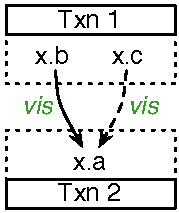
\includegraphics[width=0.25\columnwidth]{Figures/TxnAtomic}}
\hfill
\subfigure[Monotonic Atomic View]{\label{fig:txn_mav}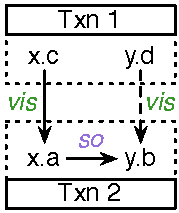
\includegraphics[width=0.25\columnwidth]{Figures/TxnMAV}}
\hfill
\subfigure[Repeatable Read]{\label{fig:txn_rr}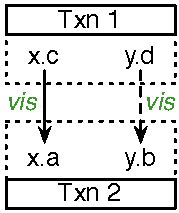
\includegraphics[width=0.25\columnwidth]{Figures/TxnRR}}
\caption{Semantics of transaction contracts. $x$ and $y$ are distinct objects.
The dotted line represents the visibility requested by the contracts.}
\label{fig:transaction}
\end{figure}

In order to illustrate the utility of transaction contract classification, we
identify three well-understood coordination-free transaction semantics -- Read
Committed (RC)~\cite{Berenson95}, Monotonic Atomic View (MAV)~\cite{BailisHAT}
and Repeatable Read (RR)~\cite{Berenson95}, and illustrate the classification
strategy. Our technique can indeed be applied to a different isolation level
lattice.

A transaction with ANSI RC semantics only witnesses committed operations. Let
us assume that the store buffers updates until all the updates from the
transaction are available at a replica. If the transaction commits, the
buffered updates are made visible. Otherwise, the buffered updates are
discarded. RC does not entail any further isolation guarantees. Hence, a store
implementing RC does not require inter-replica coordination. We can express RC
as follows:
\begin{mathpar}
\begin{array}{l}
\rcc = \forall a,b,c.~\txn{a}{b,c} \wedge \sameobj{b}{c} ~\wedge~ \vis{b}{a} \Rightarrow \vis{c}{a}
\end{array}
\end{mathpar}

\noindent Notice that the above definition is the same as the atomicity
guarantee of transaction described in Section~\ref{q_sec:syn_sem_ext}. The
\cf{save} is an example for RC transaction.

MAV semantics ensures that if some operation in a transaction $T_1$ witnesses
the effects of another transaction $T_2$, then subsequent operations in $T_1$
will also witness the effects of $T_2$. MAV semantics is useful for
maintaining the integrity of foreign key constraints, materialized views and
secondary updates. In order to implement MAV, a store only needs to keep track
of the set of transactions $S_t$ witnessed by the running transaction, and
before performing an operation at some replica, ensure that the replica
includes all the transactions in $S_t$. Hence, MAV is coordination-free. MAV
semantics is captured with the following contract:
\begin{mathpar}
\begin{array}{l}
\mavc = \forall a,b,c,d.~\txn{a,b}{c,d} ~\wedge~ \so{a}{b} ~\wedge~ \vis{c}{a} ~\wedge~ \sameobj{d}{b} \Rightarrow \vis{d}{b}
\end{array}
\end{mathpar}

\noindent whose semantics is illustrated in the Figure~\ref{fig:txn_mav}.

ANSI RR semantics requires that the transaction witness a snapshot of the data
store state. Importantly, this snapshot can be obtained from any replica, and
hence RR is coordination-free. An example for such a transaction is the
\cf{totalBalance} transaction. The semantics of RR is captured by the following
contract:
\begin{mathpar}
\begin{array}{l}
\rrc = \forall a,b,c,d.~\txn{a,b}{c,d} ~\wedge~ \vis{c}{a} ~\wedge~ \sameobj{d}{b} \Rightarrow \vis{d}{b}
\end{array}
\end{mathpar}

\noindent whose semantics is illustrated in the Figure~\ref{fig:txn_rr}.

\subsection{Classification}

Similar to operation-level contracts, with respect to $\le$ relation, the
coordination-free transaction semantics described here form a total order:
$\rcc \le \mavc \le \rrc$. The transaction classification is also similar to
the operation-level contract classification presented in
Figure~\ref{sem:classify}; given a contract $\psi$ on a transaction, we start
from the weakest transaction contract $\rcc$, and progressively compare its
strength to the known transaction contracts until we find a isolation level
under which $\psi$ can be safely discharged. Otherwise, we report a type error.

\section{Implementation}
\label{q_sec:impl}

\quelea is implemented as a shallow extension of GHC Haskell and runs on top of
Cassandra, an off-the-shelf eventually consistent distributed data (or backing)
store responsible for all data management issues (i.e., replication, fault
tolerance, availability, and convergence).  Template Haskell is used implement
static contract classification, and proof obligations are discharged with the
help of the Z3~\cite{Z3} SMT solver. Figure~\ref{fig:impl_mod} illustrates the
overall system architecture.

\begin{figure}
\begin{center}
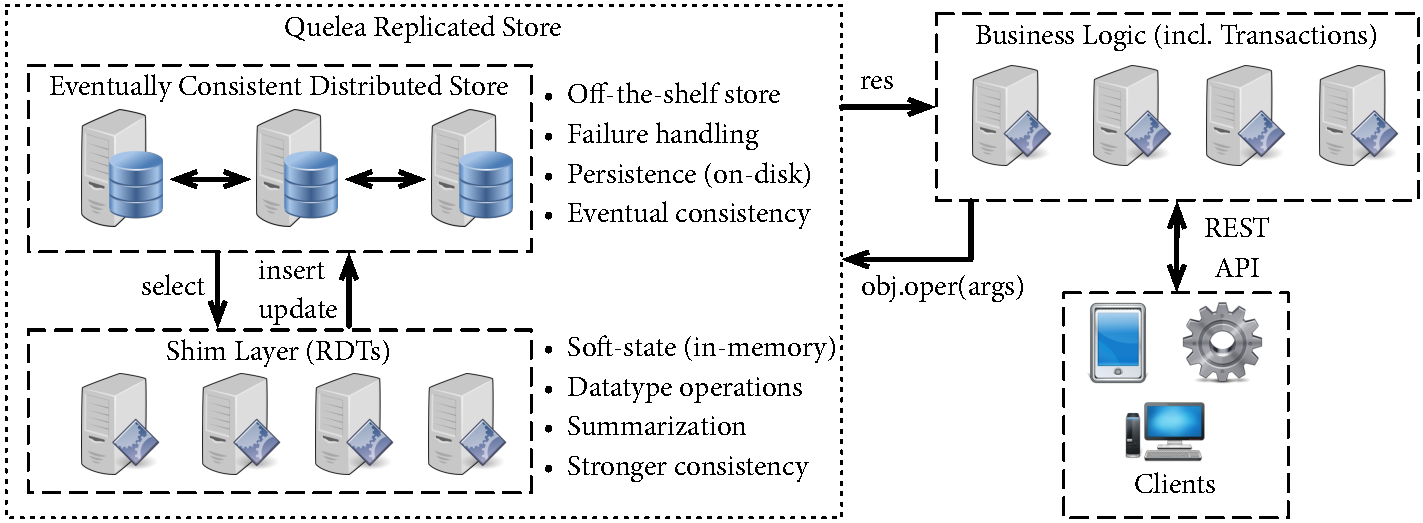
\includegraphics[width=\columnwidth]{Figures/ImplModel}
\end{center}
\caption{Implementation model.}
\label{fig:impl_mod}
\end{figure}

Replicated data types and the stronger consistency semantics are implemented
and enforced in the \emph{shim layer}. Our implementation supports eventual,
causal, and strong consistency for data type operations, and RC, MAV, and RR
semantics for transactions.  This functionality is implemented entirely on top
of the standard interface exposed by Cassandra. From an engineering
perspective, leveraging an off-the-shelf data store enables an implementation
comprising roughly only 2500 lines of Haskell code, which is packaged as a
library.

\subsection{Shim Layer}

The shim layer maintains a causally consistent in-memory snapshot of a subset
of objects in the backing store, by explicitly tracking dependencies introduced
between the effects due to visibility, session and same transaction relations.
The dependence tracking is similar to the techniques presented in~\cite{BoltOn}
and~\cite{Eiger}, with the usual optimizations making use of transitivity
properties for minimizing the number of dependencies. Shim layer performs the
reductions associated with replicated datatype operations corresponding to
client requests. As the backing store provides durability, convergence and
fault tolerance, each shim layer node simply acts as a soft-state cache, and
can safely be terminated at any instant. Similarly, more shim layer nodes can
be spawned on demand.

\subsection{Operation Consistency}

Every effect generated as a result of an effectful operation on an object
inserts a new row $(o,e,vis,txn,val)$ into the backing store, where $o$ and $e$
are object and (unique) effect identifiers, $vis$ is the set of identifiers of
effects visible to this operation, $txn$ is an optional transaction identifier,
and $val$ is the value associated with the effect (eg: \cf{Withdraw 50}). The
shim layer periodically fetches updates from the backing store for those objects
which were accessed since updates were last fetched. Since causally consistent
operations require an up-to-date view of the current session, the shim layer
node synchronously fetches operations if the causally preceding operations in
the current session are not available in the cache.  Strongly consistent
operations are performed after obtaining exclusive leases on objects. The lease
mechanism is implemented with the help of Cassandra's support for conditional
updates and expiring columns.

\subsection{Transactions}

While Cassandra offers all-or-nothing failure semantics for multiple writes
through batching, readers may witness the initial write while the batch is in
progress. \quelea implements atomic visibility by exploiting shim layer causality
guarantee -- an effect is included only if all the effects if depends on are
also included.

\begin{figure}[t]
\begin{center}
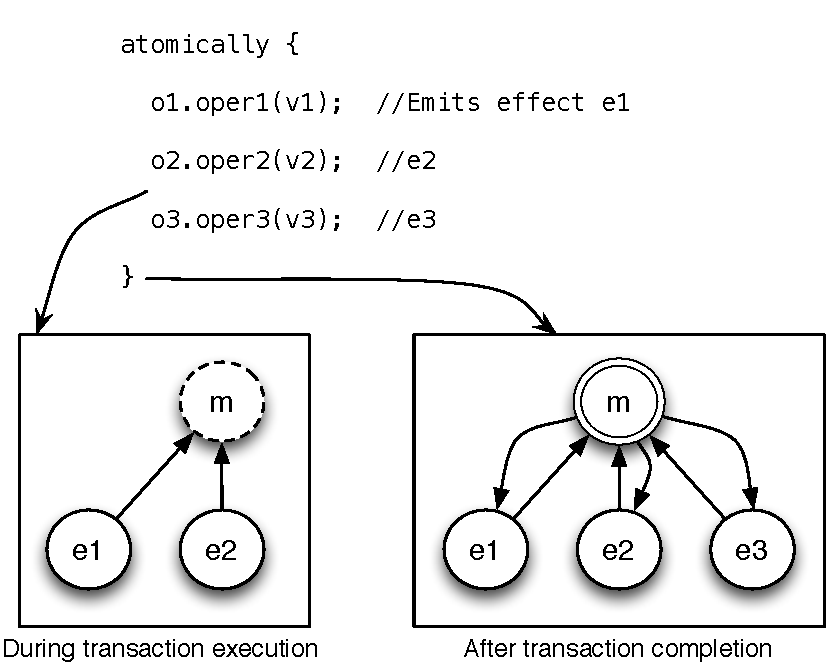
\includegraphics[width=0.7\columnwidth]{Figures/AtomicityImpl}
\end{center}
\caption{Implementing atomicity semantics. Dotted circle represents effects not yet inserted into the backing store.}
\label{fig:atomicity_impl}
\end{figure}

Consider the example given in Figure~\ref{fig:atomicity_impl}. For every
transaction in \quelea, we instantiate a special transaction marker effect $m$.
But importantly, do not insert into the backing store. $m$ is included as a
dependence to every effect generated in the transaction. In the figure, the
graph on the left shows the state of the store in the middle of a transaction.
Each circle represents an effect. The dotted circle indicates that the effect
has been instantiated, but has not yet been inserted into the store. Since the
causally preceding effect $m$ has not yet been written to the store, no
operation will witness $e1$ and $e2$ while the transaction in progress. After
the transaction has finished execution, we insert $m$ into the backing store,
marking all the effects from the transactions as a depedence for $m$. Now any
replica which includes one of the effects from the transaction must include
$m$, and transitively must include every effect from the transaction. This
ensures atomicity and satisfies the RC requirement.

The above scheme prevents a transaction from witnessing its own effects. This
might conflict with the causality requirement on the operations. Hence,
transactions piggy-back the previous effects from the same transaction for each
request. MAV semantics is implemented by keeping track of the set of
transaction markers $M$ witnessed by the transaction, and before performing an
operation at some replica, ensuring that $M$ is a subset of the transaction
markers included at that replica. If not, the missing effects are synchronously
fetched. RR semantics is realized by capturing a optimized snapshot of the
state of some replica; each operation from an RR transaction is applied to this
snapshot state. Any generated effects are added to this snapshot.

\subsection{Summarization}

The main challenge in realizing an efficient implementation of operation-based
replicated data types is that the state of the object i.e., the set of effects
grows with every effectful operation on the object. If left unchecked, the
operations slow down over time, until the shim layer memory or backing store
disk runs out of memory. Luckily, the state of the operation-based replicated
data type can often be summarized to an \emph{observably equivalent} smaller
state. For example,

\begin{itemize}
\setlength{\itemsep}{2pt}
\item A last-writer-wins register with multiple updates where $v$ is the value
of the last write is observably equivalent to a register with a single write
$v$.

\item A bank account with a series of deposits and withdraws with current
balance $b$ is equivalent to a bank account with a single deposit of $b$.

\item A set with collection of add and remove operations is equivalent to a set
with a series of add operations of live elements from the original set.
\end{itemize}

Since the semantics of summarization depends on the semantics of the data type,
we expect the programmer to provide a summarization function for each RDT with
the following type:

\begin{codehaskell}
summarize :: [e] -> [e]
\end{codehaskell}

\noindent with the intention that the length of the result is smaller that the
length of the argument. We utilize the \cf{summarize} function to summarize the
object state both in the shim layer node and the backing store, typically when
the number of effects on an object crosses a tunable threshold. Shim layer
summarization is straight-forward; a summarization thread takes the local lock
on the object, and replaces its state with the summarized state. The shim layer
node remains unavailable for that particular object during summarization
(usually a few milliseconds).

Compared to the shim layer, summarization in the backing store is more
complicated. The main challenge is that unlike the shim layer, summarization
cannot run as an atomic operation. Summarization in the backing store involves
deleting previously inserted rows and inserting new rows, where each row
corresponds to an effect. It is essential that concurrent client operations are
permitted, but are not allowed to witness the intermediate state of the
summarization process.

\begin{figure}[t]
\begin{center}
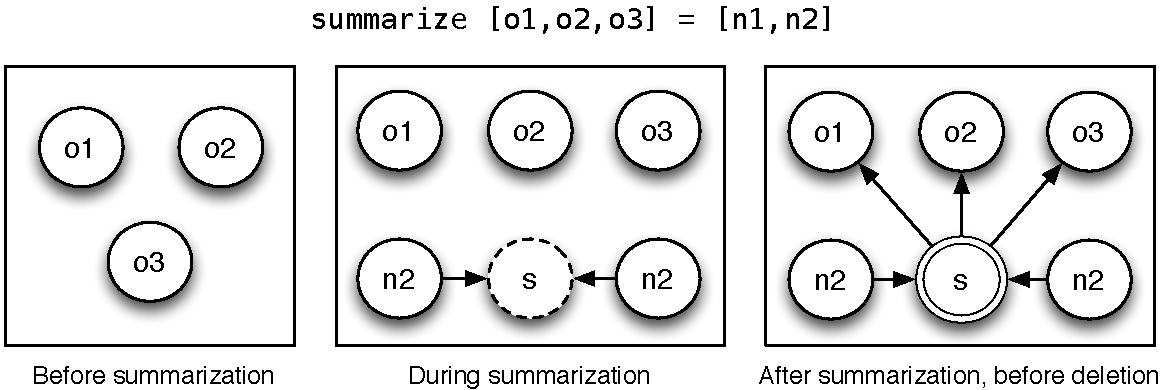
\includegraphics[width=\columnwidth]{Figures/SumDisk}
\end{center}
\caption{Summarization in the backing store. Dotted circle represents effects not yet inserted into the backing store.}
\label{fig:impl_sum_disk}
\end{figure}

To this end, we adopt a novel summarization strategy that builds on the
causality property of the store. Figure~\ref{fig:impl_sum_disk} illustrates the
summarization strategy. Suppose the original set of effects on an object are
$o1$, $o2$ and $o3$. Whe summarized, the new effects yielded are $n1$ and $n2$.
We first instantiate a summarization marker $s$, and similar to transaction
marker, we do not insert it into the store immediately. We insert the new
effects $n1$ and $n2$, with strong consistency, including $s$ as a dependence.
Since $s$ is not yet in the store, the new effects are not made visible to the
clients. Then we insert $s$ with strong consistency, including the original
effects $o1$, $o2$ and $o3$ as dependence. Strongly consistent insertions
ensure that a shim layer node witnessing $s$ on some object must also witness
$n1$ and $n2$ on the same object. A shim layer node which witnesses all the
effects removes the original effects from its cache since they are superseded
by the new effects. Finally, the old effects are deleted from the backing
store. This process ensures that clients either witness the old or the new
effects, but not both; the summarization process appears to be atomic from the
clients perspective.

\section{Evaluation}
\label{q_sec:results}

In this section, we evaluate \quelea programs, report their contract profile
and illustrate the performance benefits of fine-grained consistency
classification on operations and transactions. We also evaluate on the impact
of the summarization. We implemented the following applications, which includes
individual RDTs as well as larger applications composed of several RDTs:

\begin{itemize}

\item \textbf{LWW register}: A last-write-wins register that provides read and
write operations. Each write is associated with a timestamp, which is used to
resolve conflicting concurrent writes -- newer write wins.

\item \textbf{DynamoDB register}: A integer register that allows eventual and
strong puts and gets, conditional puts, increment and decrement operations.

\item \textbf{Bank account}: Our running example, with savings and current
accounts.

\item \textbf{Shopping list}: Collaborative shopping list which allows adding
and deleting items.

\item \textbf{Online store}: Models an online store with shopping cart and
dynamically changing item prices. Checkout process verifies that the customer
only pays the accepted price.

\item \textbf{RUBiS}: An ebay-like auction site~\cite{RUBiS}. The application
allows users to browse items, bid for items on sale, and pay for items from a
wallet modelled after a bank account.

\item \textbf{Microblog}: A twitter-like microblogging site, modelled after
Twissandra~\cite{Twissandra}. The application allows adding a new user, adding
and replying to tweets, following, unfollowing and blocking users, and fetching
a user's timeline, userline, followers and following.
\end{itemize}

\begin{table}[t]
\caption{The distribution of classified contracts. \#T refers to the number of
tables in the application. The columns 4-6 (7-9) represent operations
(transactions) assigned to this consistency (isolation) level.}
\begin{center}
\begin{tabular} {|l|r|r|r|r|r|r|r|r|}
\hline
{\bf Benchmark} & {\bf LOC} & {\bf \#T} & {\bf EC} & {\bf CC} & {\bf SC} & {\bf RC} & {\bf MAV} & {\bf RR} \\
\hline
{LWW Reg} & 108 & 1 & 2 & 2 & 2 & 0 & 0 & 0 \\
{DynamoDB} & 126 & 1 & 3 & 1 & 2 & 0 & 0 & 0 \\
{Bank Account} & 155 & 1 & 1 & 1 & 1 & 1 & 0 & 1 \\
{Shopping List} & 140 & 1 & 2 & 1 & 1 & 0 & 0 & 0 \\
{Online store} & 340 & 4 & 9 & 1 & 0 & 2 & 0 & 1 \\
{RUBiS} & 640 & 6 & 14 & 2 & 1 & 4 & 2 & 0 \\
{Microblog} & 659 & 5 & 13 & 6 & 1 & 6 & 3 & 1 \\
\hline
\end{tabular}
\end{center}
\label{tab:ctrts}
\end{table}

The distribution of contracts in these applications is given in
Table~\ref{tab:ctrts}. We see that majority of the operations and transactions
are classified as eventually consistent and RC, respectively. Operation
contracts are used to enforce integrity and visibility constraints on
individual fields in the tables. Transactions are mainly used to consistently
modify and access related fields across tables. In \quelea, the contract
classification process is completely performed at compile time and has no
overheads at runtime. The proof obligations associated with contract
classification is discharged through the Z3 SMT Solver. Across our benchmarks,
classifying a contract took 11.5 milliseconds on average.

For our performance evaluation, we deploy \quelea applications in
\emph{clusters}, where each cluster is composed of 5 fully replicated Cassandra
replicas within the same datacenter. We instantiate one shim layer node for
every Cassandra replica, and place it on the same VM as the Cassandra replica.
Clients are instantiated on the same data center as the store, and run
transactions. We deploy the each node in the cluster on \cf{c3.4xlarge} Amazon
EC2 instances. Our shim layer nodes are multi-threaded, and we allocate 8 CPUs
(out of 16 available) for each shim layer node. The clients also run on
\cf{c2.4xlarge} instances. We call this \cf{1DC} configuration. For our
geo-distributed experiments (\cf{2DC}), we instantiate 2 clusters, each with 5
nodes, and place the clusters on US-east (Virginia) and US-west (Oregon). The
average inter-region latency was 85ms.

\begin{figure*}[t]
  \centering
  \subfigure[Latency]{\label{grf:BA-lat}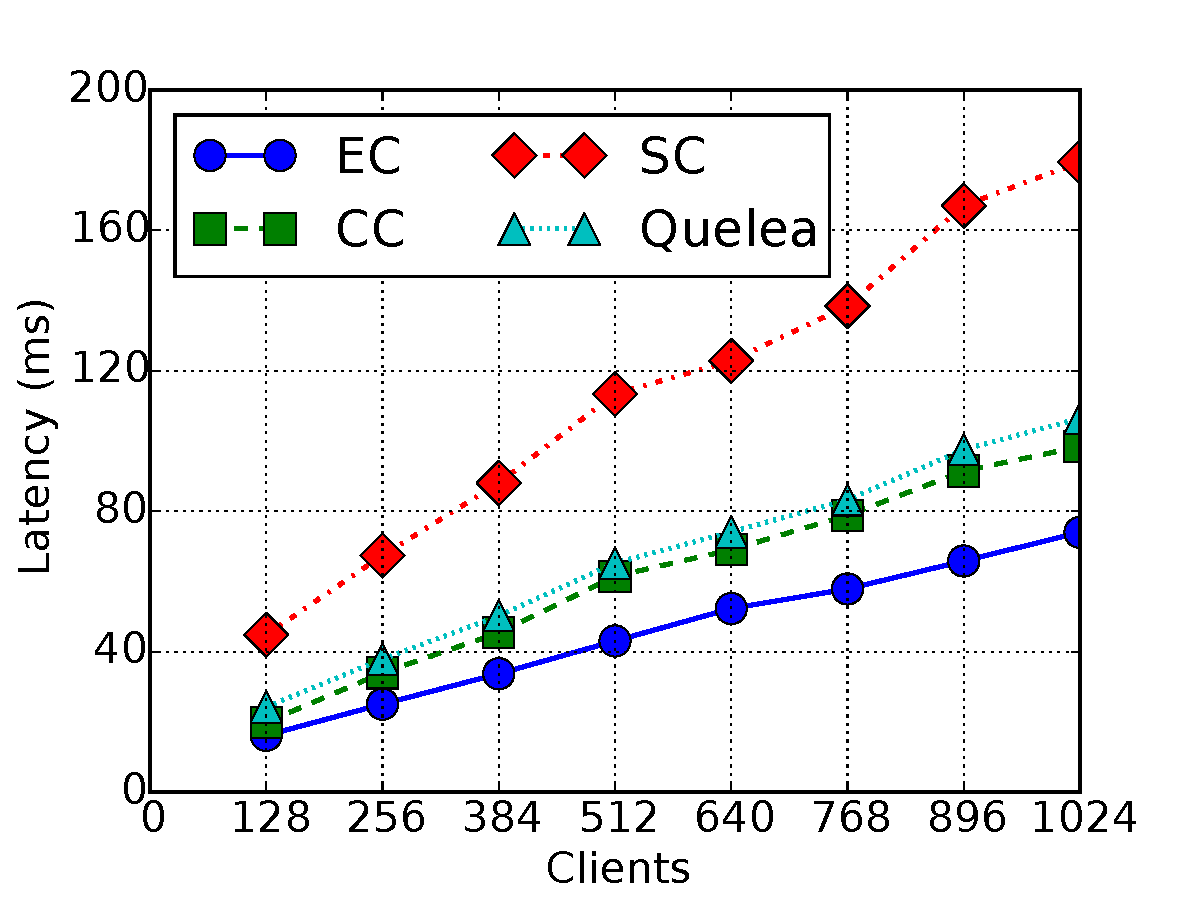
\includegraphics[width=0.45\textwidth]{graphs/BA-lat.pdf}}
  \subfigure[Throughput]{\label{grf:BA-tp}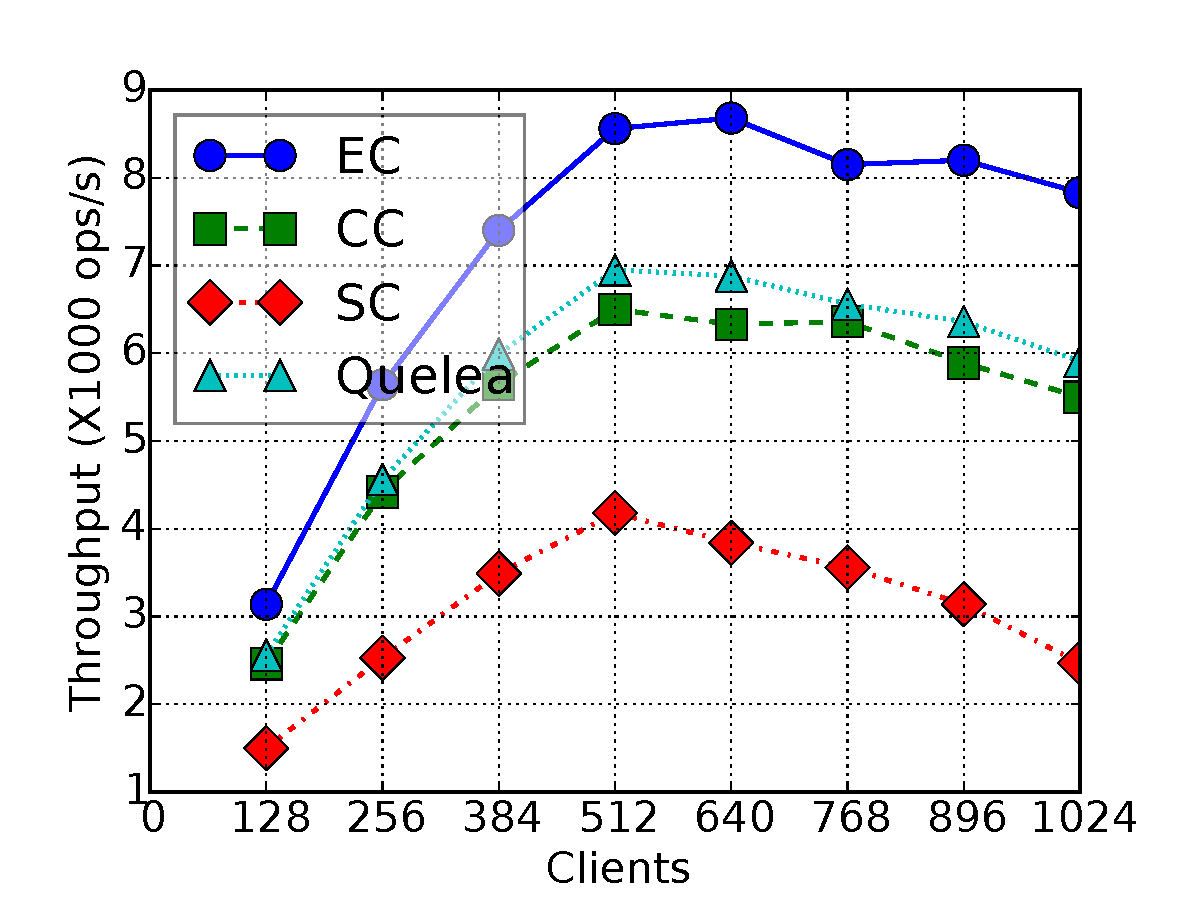
\includegraphics[width=0.45\textwidth]{graphs/BA-tp.pdf}}
  \subfigure[Throughput vs. Latency]{\label{grf:BA-tp-vs-lat}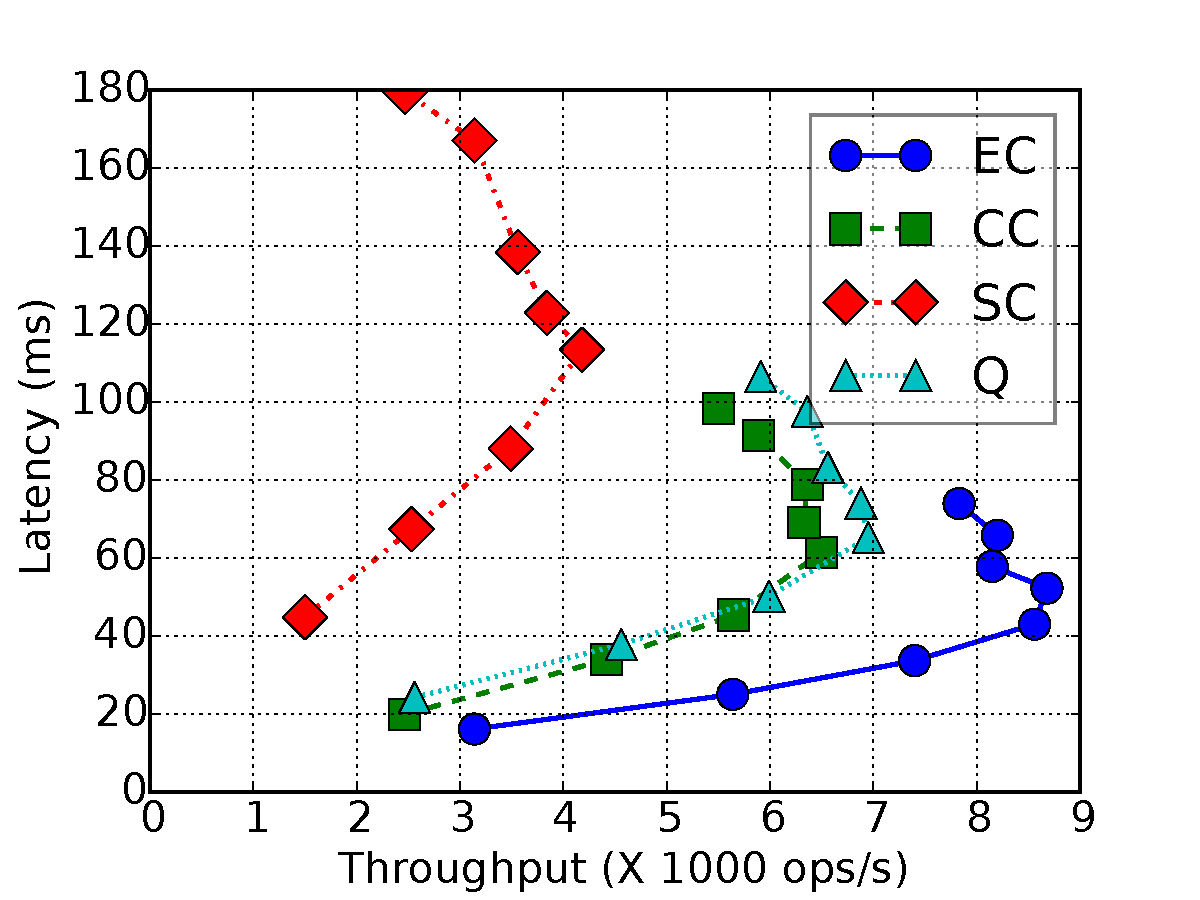
\includegraphics[width=0.45\textwidth]{graphs/BA-tp-vs-lat.pdf}}
	\caption{Bank account performance.}
  \label{grf:BA}
\end{figure*}


Figure~\ref{grf:BA} shows the performance of operations in bank account example
as we increase the number of clients in \cf{1DC} configuration. Our client
workload was generated using YCSB benchmark~\cite{YCSB}. The benchmark
uniformly chose from 100,000 keys, where the operation spread was 25\%
withdraw, 25\% deposit and 50\% getBalance, which corresponds to the default
50:50 read:write mix in YCSB. We increased the number of clients from 128 to
1024, and each experiment ran for 180 seconds.

The lines marked EC and CC correspond to all operations being assigned EC and
CC consistency levels. These levels compromise correctness as withdraw has to
be and SC operation. The line SC corresponds to a configuration where all
operations are strongly consistent; this ensures application correctness.
\quelea corresponds to our implementation, which classifies operations based on
their contracts. Both \quelea and SC ensure correctness. However, with 512
clients, \quelea implementation was within 41\% of latency and 18\% of
throughput of EC, whereas SC operations had 162\% higher latency and 52\% lower
throughput than EC operations. Observe that in the
Figure~\ref{grf:BA-tp-vs-lat} which compares throughput vs. latency, there is a
point in each case after which the latency increases while the throughput
decreases. This indicates a point after which the store becomes saturated with
client requests.

In \cf{2DC} configuration (not-shown), the average latency of SC operations
with 512 clients increased by 9.4$\times$ due to the cost of geo-distributed
coordination, whereas \quelea operations were only 2.2$\times$ slower, mainly
due to the increased cost of \cf{withdraw} operations. Importantly, the latency
of \cf{getBalance} and \cf{deposit} remained almost the same. This illustrates
the benefit of fine-grained contract classification in \quelea.

\begin{figure*}[t]
  \centering
  \subfigure[Latency]{\label{grf:LWW-txn-lat}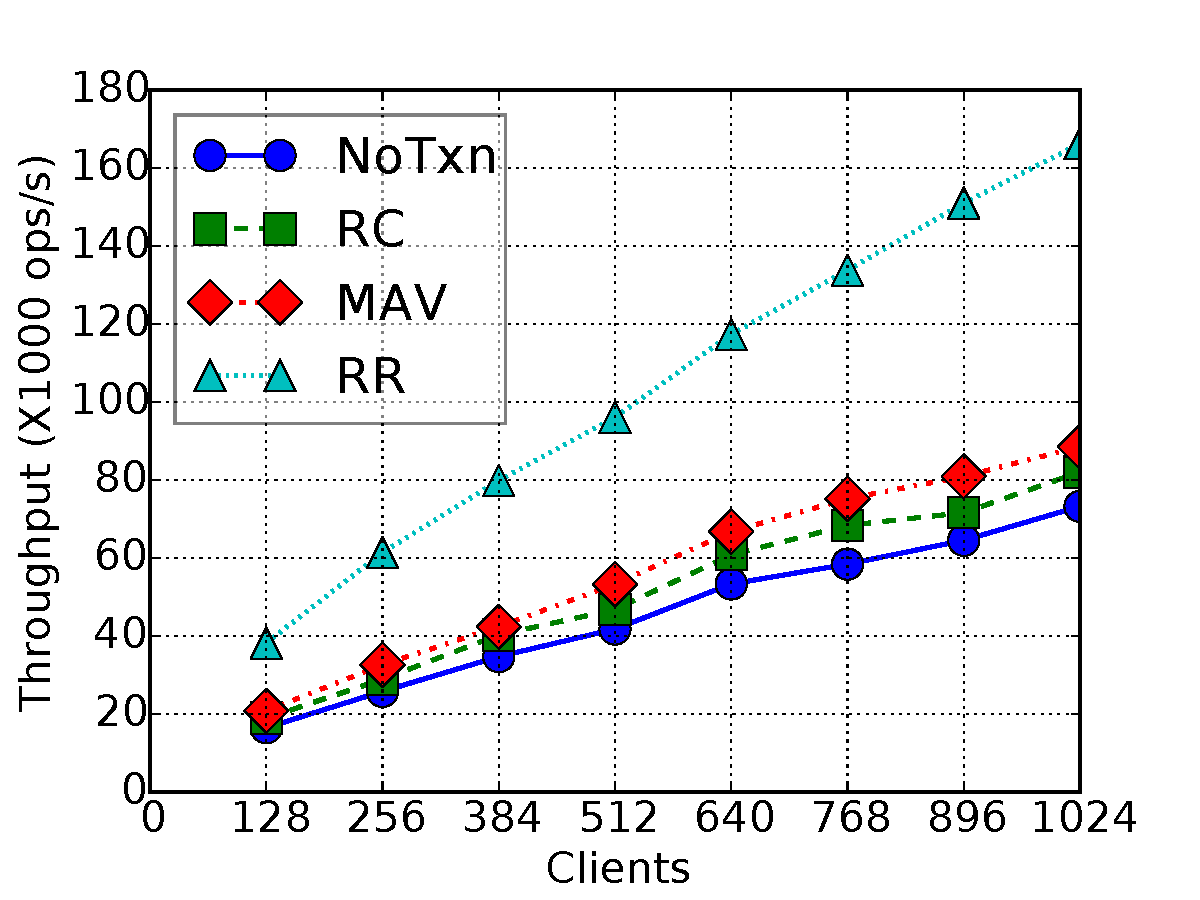
\includegraphics[width=0.45\textwidth]{graphs/LWW-txn-lat.pdf}}
  \subfigure[Throughput]{\label{grf:LWW-txn-tp}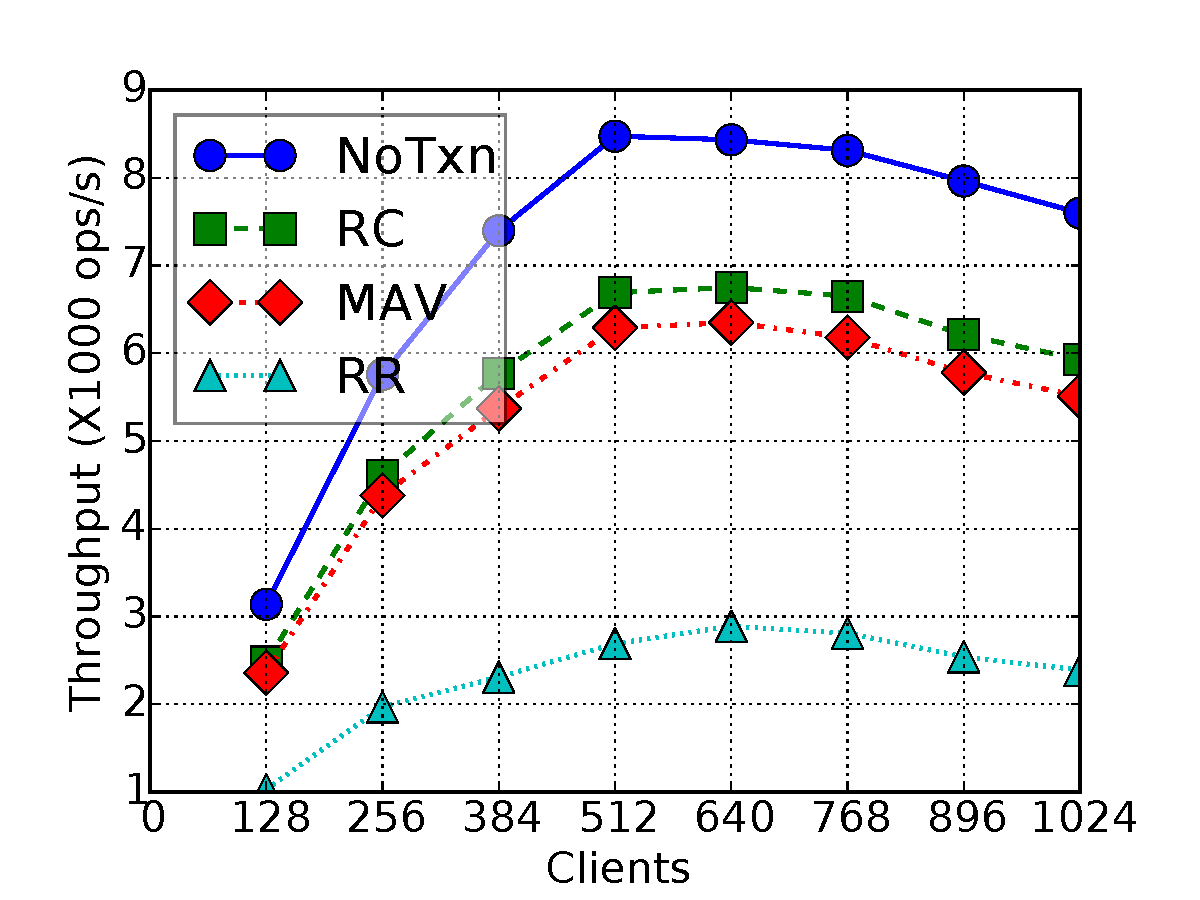
\includegraphics[width=0.45\textwidth]{graphs/LWW-txn-tp.pdf}}
  \subfigure[Throughput vs. Latency]{\label{grf:LWW-txn-tp-vs-lat}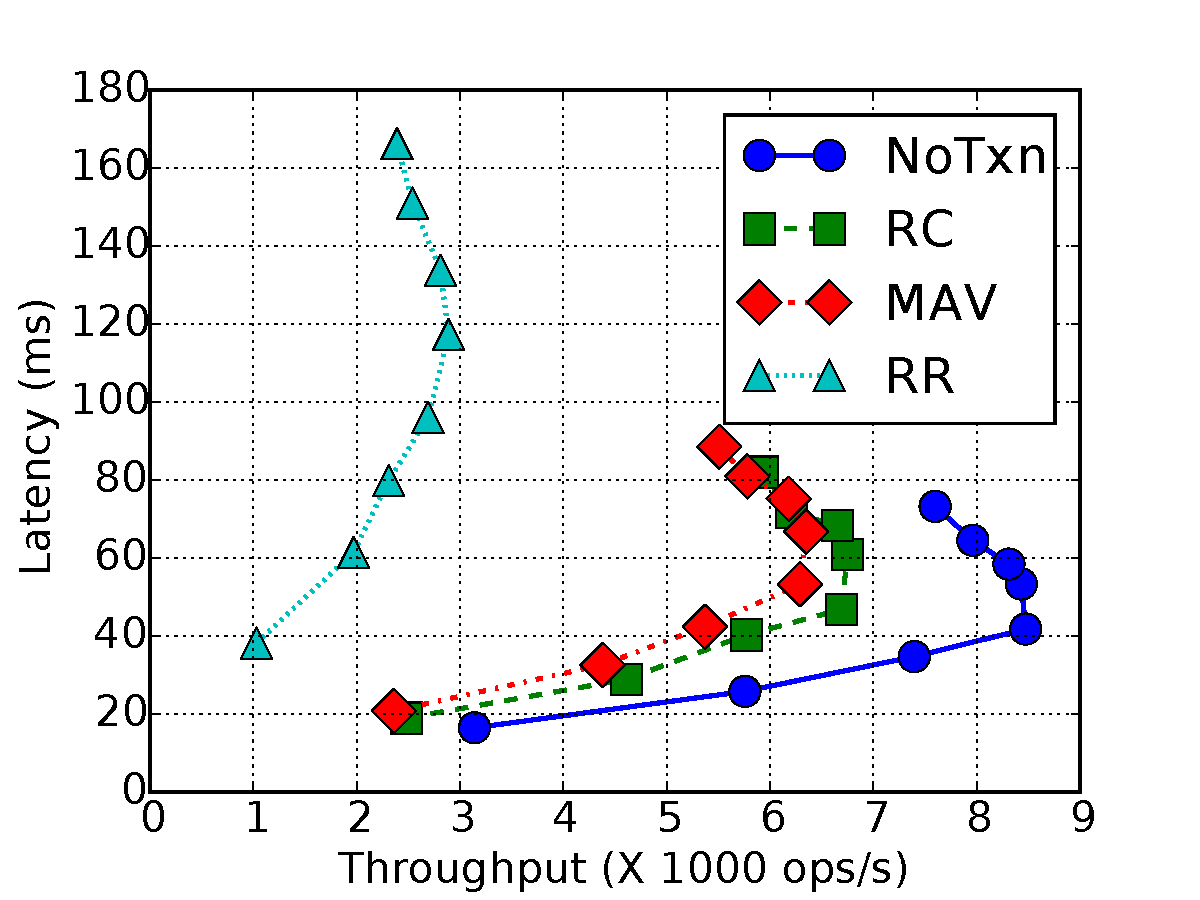
\includegraphics[width=0.45\textwidth]{graphs/LWW-txn-tp-vs-lat.pdf}}
	\caption{LWW register transaction performance.}
  \label{grf:LWW-txn}
\end{figure*}

We compare the performance of different transaction isolation level choices in
Figure~\ref{grf:LWW-txn} using the LWW register. The numbers were obtained
under 1DC configuration. The YCSB workload was modified to issue 10 operations
per transaction, with the default 50:50 read:write mix. Each operation is
assumed to have eventual consistency. \cf{NoTxn} corresponds to a configuration
that does not use transactions. Compared to this RC is only 12\% shower in
terms of latency with 512 clients, where as RR is 2.3X slower. The difference
between RC and \cf{NoTxn} is due to the meta-data overhead of recording
transaction information in the object state. For RR transaction, the cost of
capturing and maintaining the snapshot in an RR transaction is the biggest
source of overhead.

We also compared (not shown) the performance of EC LWW operations directly
against Cassandra (our backing store), which uses last-writer-wins as the only
convergence semantics. While Cassandra provides no stronger-than-eventual
consistency properties, \quelea was within 30\%(20\%) of latency(throughput) of
Cassandra with 512 clients, illustrating that the programmers only have to pay
a minimal overhead for the expressive and stronger \quelea programming model.

\begin{figure}[t]
  \centering
  \subfigure[Latency]{\label{grf:rubis-lat}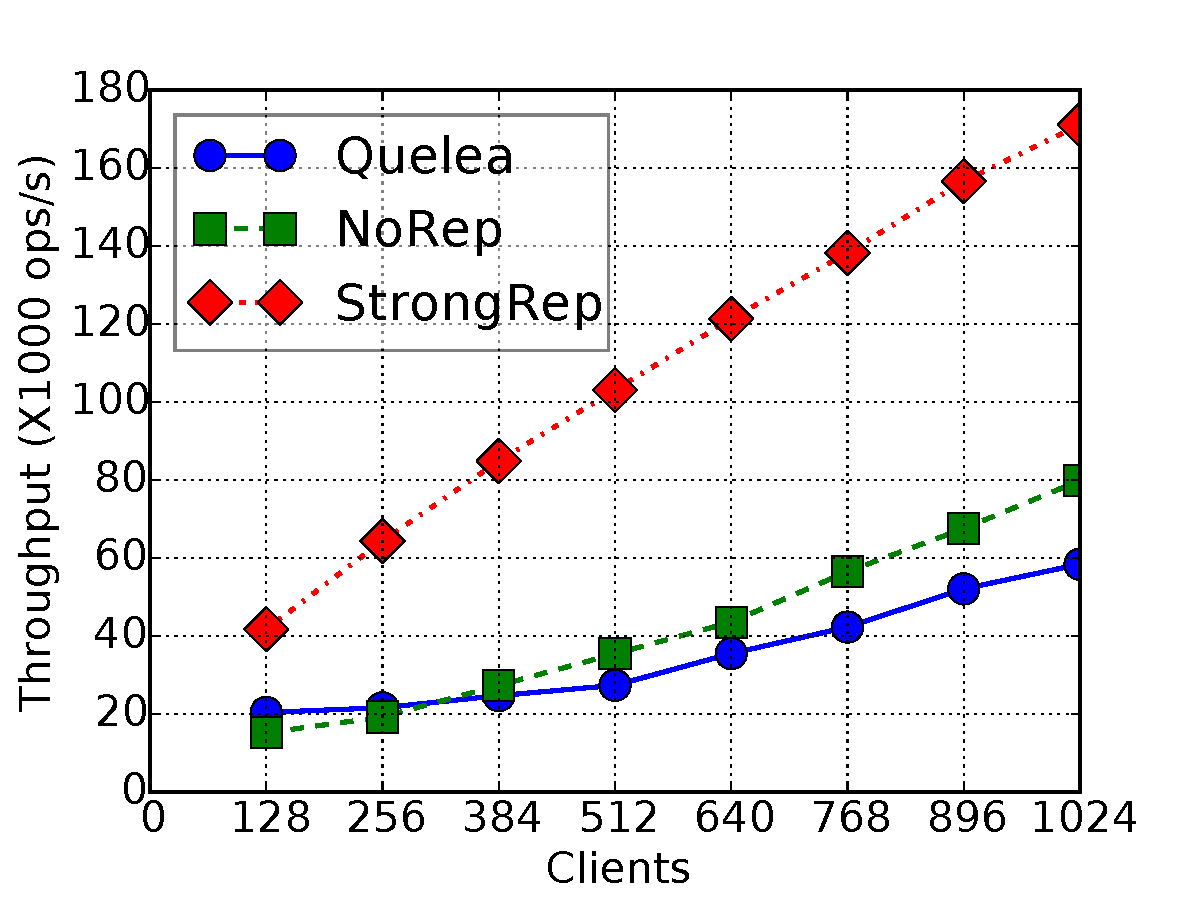
\includegraphics[width=0.45\textwidth]{graphs/Rubis-lat.pdf}}
  \subfigure[Throughput]{\label{grf:rubis-tp}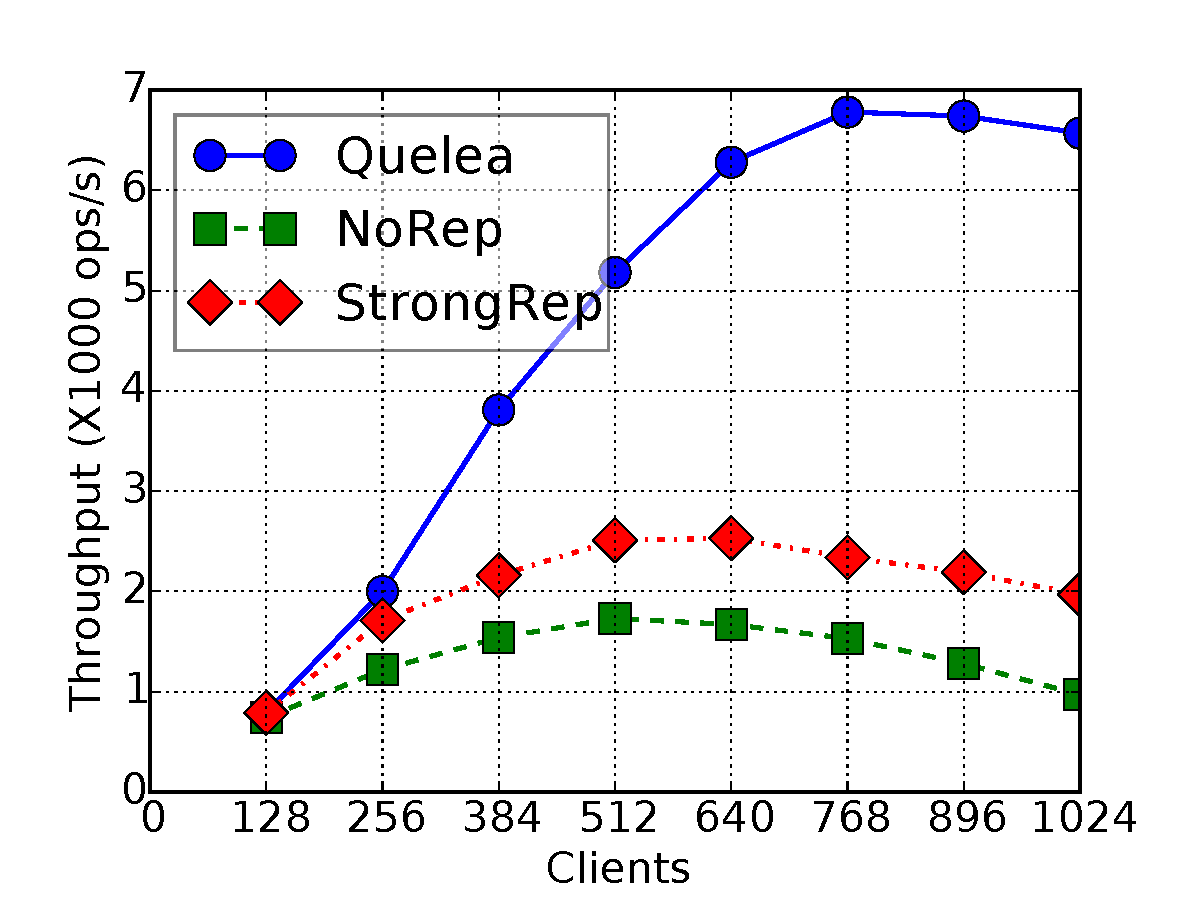
\includegraphics[width=0.45\textwidth]{graphs/Rubis-tp.pdf}}
  \subfigure[Throughput vs. Latency]{\label{grf:Rubis-tp-vs-lat}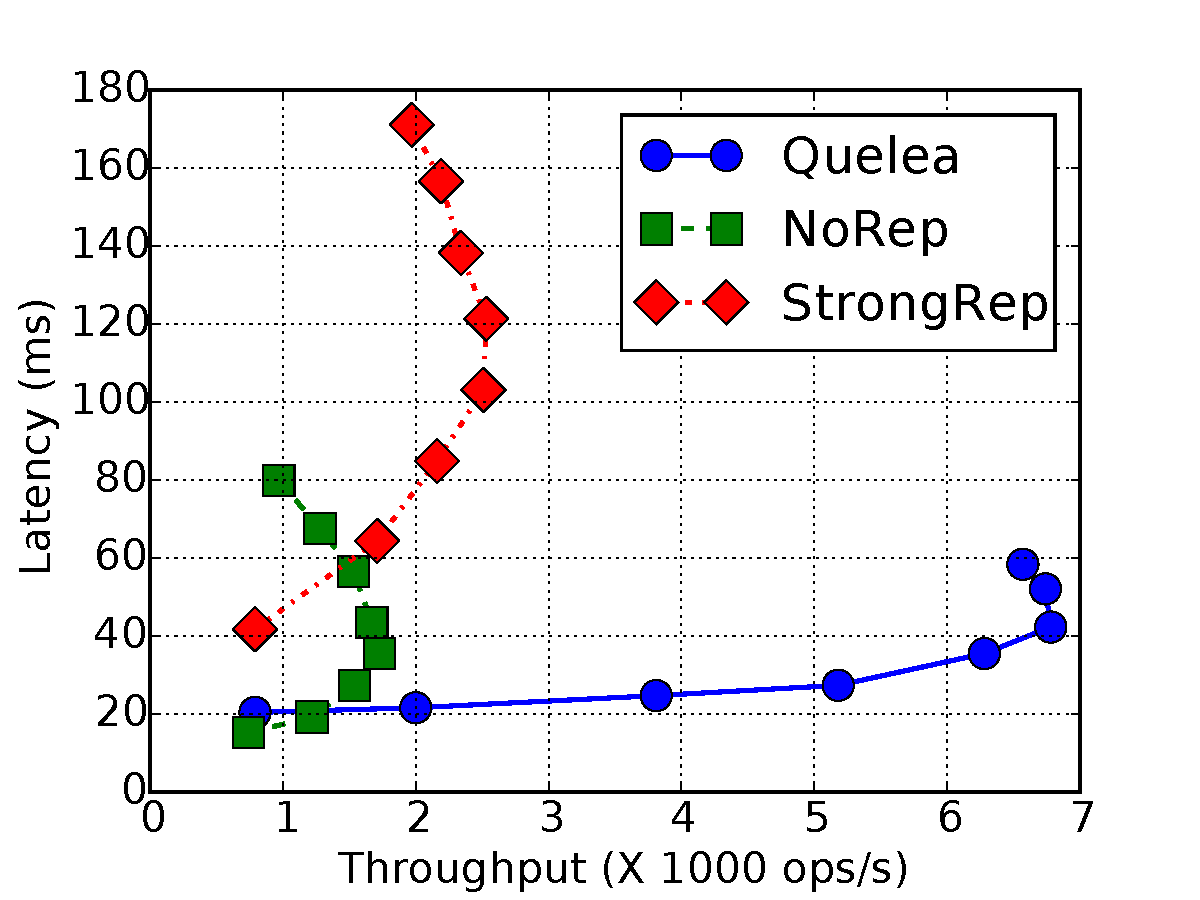
\includegraphics[width=0.45\textwidth]{graphs/Rubis-tp-vs-lat.pdf}}
	\caption{Rubis bidding mix performance.}
  \label{grf:rubis}
\end{figure}


Figure~\ref{grf:rubis} compares the \quelea implementation of RUBiS in \cf{1DC}
configuration against a single replica (NoRep) and strongly replicated
(StrongRep) \cf{1DC} deployment. The benchmark was RUBiS bidding mix, which has
15\% read-write interactions, which is representative of the auction workload.
Without replication, NoRep trivially provides strong consistency. However, this
deployment does not scale beyond 1750 operations per second. Strong replication
offers better throughput at the cost of greater latency due to inter-replica
coordination. \quelea deployment offers the benefit of replication, while only
paying the cost of coordination when necessary.

\begin{figure}[t]
\centering
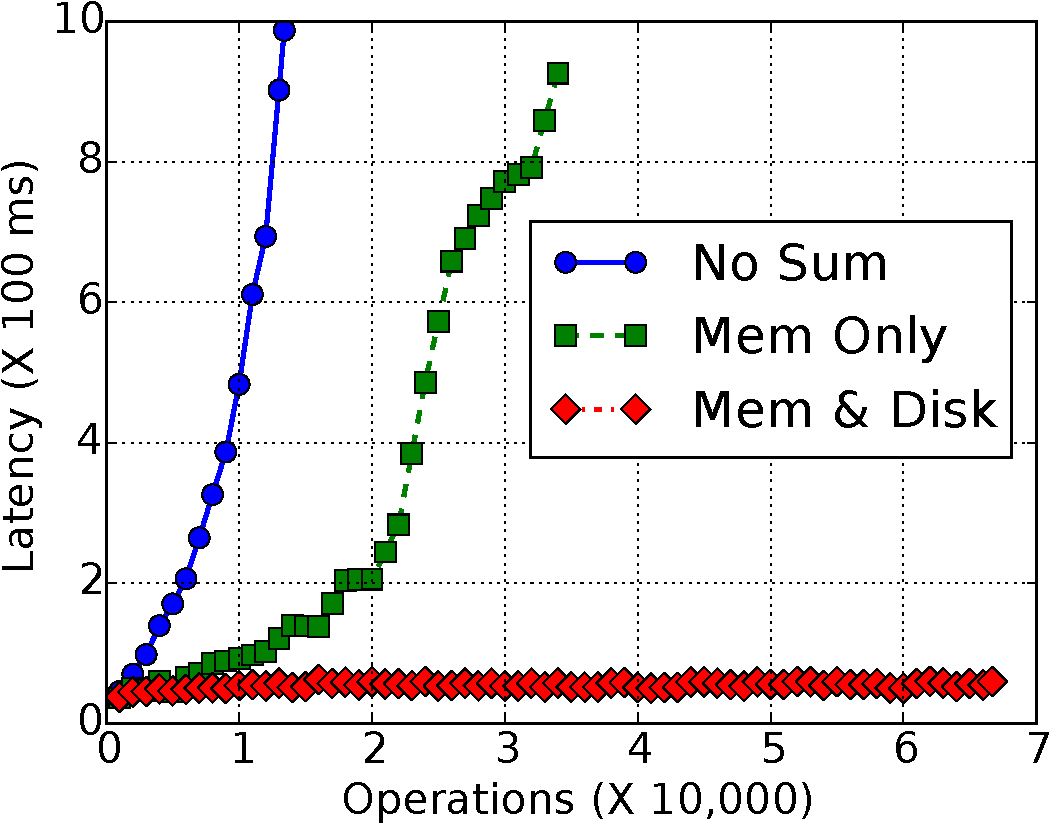
\includegraphics[width=0.45\textwidth]{graphs/summarization.pdf}
\caption{Impact of summarization.}
\label{grf:summarization}
\end{figure}

Finally, we study the impact of summarization in
Figure~\ref{grf:summarization}. We utilize 128 clients and a single \quelea
replica, with all the clients operating on the \emph{same} LWW register to
stress test the summarization mechanism. The shim layer cache (mem) of
operations is summarized every 64 updates, while the updates in the backing
store (disk) are summarized every 4096 updates. Each point in the graph
represents the average latency of the previous 1000 operations. Each experiment
is run for 60s.

The results show that without summarization, the average latency of operations
increase exponentially to almost 1 second, and only 13K operations were
performed in a minute. Since every operation has to reduce over the set of all
previous operations, with a ever growing set, the operations take increasingly
more time to complete. With summarization only in memory, the performance still
degrades due to the cost of fetching all previous updates from the backing
store into the shim layer. Fetching the latest updates is essential for SC
operations. With both summarizations enabled, we see that the latency does not
increase over time, and we were able to perform 67K operations. This graph
illustrates the importance and effectiveness of summarization in \quelea.

\section{Related Work}
\label{q_sec:related}

Operation-based RDTs have been widely studied in terms of their algorithmic
properties~\cite{SSS,Burckhardt2014}, and several systems utilize this model to
construct distributed data structures~\cite{Lakshman2010,Bayou,Tango}. These
systems typically propose to implement the datatypes directly over a cluster of
nodes, and only focus on basic eventual consistency. Hence, these systems
implement custom solutions for durability and fault-tolerance. \quelea realizes
RDTs stronger consistency models on top of off-the-shelf eventually consistent
distributed stores. In this respect, \quelea is similar to~\cite{BoltOn} where
causal consistency is achieved through a shim layer on Cassandra, which
explicitly tracks and enforces dependencies between updates.
However,~\cite{BoltOn} does not support user-defined RDTs, automatic contract
classification and transactions.

Since eventual consistency alone is insufficient to build correct applications,
several systems~\cite{Bayou,Terry2013,RedBlue} propose a lattice of stronger
consistency levels. Similarly, traditional database processing
systems~\cite{Berenson95} and their replicated variants~\cite{BailisHAT}
propose weaker isolation levels for performance. In these systems, the onus is
on the developer to choose the correct consistency(isolation) level for
operations(transactions). \quelea relieves the developer of this burden, and
instead expects contracts expressing declarative visibility requirements.

Our contract language is inspired by the axiomatic description of RDT semantics
proposed by~\cite{Burckhardt2014}. While they use axioms for formal
verification of correctness of an RDT implementation, we utilize them as a
means for the user to express the desired consistency guarantees in the
application. Similar to their work, our contract language does not incorporate
real (i.e., wall-clock) time. Hence, it cannot describe store semantics such as
recency or bounded-staleness guarantees offered by certain
stores~\cite{Terry2013}.

Several conditions have been proposed to judge whether an operation on a
replicated data object needs coordination or not. ~\cite{Calm} defines
\emph{logical monotonicity} as a sufficient condition for coordination freedom,
and proposes a consistency analysis that marks code regions performing
non-monotonic reasoning (eg: aggregations, such as \cf{COUNT}) as potential
coordination points.  ~\cite{IConfluence} and ~\cite{Sieve} define
\emph{invariant confluence} and \emph{invariant safety}, respectively, as
conditions for safely executing an operation without coordination. ~\cite{Sieve}
also proposes a program analysis that conservatively marks operations as
\emph{blue} (coordination not required), while marking the remaining as
\emph{red} (coordination required). Unlike \quelea, these works focus on a
coarse-grained classification of consistency as eventual or strong, and do not
focus on transaction isolation levels. However, program analyses they propose
relieve programmers of the burden to tag operations with consistency levels.
Indeed, we do consider automatic inference of consistency contracts from
application-specific integrity constraints as the next step for \quelea.

\section{Concluding Remarks}
\label{q_sec:concl}

In this chapter, we have presented \quelea a shallow Haskell extension for
declarative programming over eventually consistent data stores. The key idea of
\quelea is the automatic classification of fine-grained consistency contracts on
operations and distributed transactions with respect to the consistency and
isolation levels offered by the store. Our contract language is carefully
crafted from a decidable subset of first-order logic, enabling the use of
automatic theorem prover to discharge the proof obligations associated with
contract classification. We realize an instantiation of \quelea on top of
off-the-shelf distributed store, Cassandra, and illustrate the benefit of
fine-grained contract classification by implementing and evaluating several
scalable applications.


% Summary and/or conclusions are optional but often used.
% The summary and/or conclusions often are the last
% the last major division(s) of the text.
% Reference: TM2006 page 32.
% CHANGE NEXT LINE?
\chapter{Concluding Remarks and Future Work}
\label{chap:conclusion}

A strongly consistent view of data, which enables the programmer to treat
parallel and distributed architectures as a centralized system, is at odds with
practical concerns such as availability, coherence, latency, and partial
failures. Hence, modern multicore and distributed systems only provide weak
consistency guarantees, belying the semblance of a centralized system, which
complicates concurrent programming. In this dissertation, we presented three
novel techniques for programming under weak consistency. \MMSCC provides a
coherent and managed shared memory for programmers on the non-cache coherent
Intel SCC processor. \rxcml enables synchronous communication to be utilized as
an abstraction over asynchronous distributed systems. \quelea permits
declarative reasoning about consistency guarantees for programs over eventually
consistent data stores.

In this chapter, we present the future work. This discussion is split based on
the three contributions.

\section{\MMSCC}

The main hindrance to scalability of our \MMSCC collector is the stop-the-world
nature of the shared heap collection. While shared heap collections are
infrequent when compared to local collections, the pause time for shared heap
collections reaches almost one second due to (1) the uncached nature of the
collection and (2) the cost of synchronizing all the cores on a barrier. A
natural extension to address this issue is to make the shared heap collection
concurrent similar to the design by Doligez et al.~\cite{Doligez93}. In a
concurrent shared heap collection, the cores no longer need to synchronize on a
global barrier, and we could envision allocating a few of the available cores
specifically for concurrent shared heap collection.

Our globalization strategy lifts the \emph{entire} transitive closure of the
globalized object to the shared heap. We have observed that this strategy
although simple to implement, globalizes far more memory than is actually
shared between the cores. This phenomenon has also been observed by Marlow et
al.~\cite{Marlow11} in their local collector design for Haskell. We can
envision a strategy where only portions of the transitive closure are
globalized, with further globalization on demand. In this design, we will have
pointers from shared heap into local heaps (breaking the heap invariant). We
can treat such pointers similar to remembered
stacks (Section~\ref{sec:aneris_rem_stack}), adding the pointers into the local heap
into a remembered set, so that they can be traced during local GCs. Moreover,
the abundance of concurrency in our programming model can mask the latency
associated with on-demand globalization, which involves cross-core
communication.

Finally, while our GC design is geared for circumventing the absence of cache
coherence, we get the added benefit of reduced pause times since each local
heap is collected independently. However, our local heap collections are indeed
optimized for throughput and optimal memory utilization. If latency is indeed
the desired metric, we can envision concurrent and incremental collection for
the local heaps. In particular, the independence of collection in the local
heaps in \MMSCC allows the same execution to utilize latency sensitive GC in a
collection of cores with throughput optimized GC in others. Thus, \MMSCC
design is well-suited for mixed mode applications such as web-browsers, where
both latency and throughput are important for distinct parts of the same
program.

\section{\rxcml}

While \rxcml provides composable synchronous reasoning for asynchronous
distributed systems, the implementation does not address the challenge of
partial failures in such a setting. The key observation we make is that the
dependence graph used for monitoring the correctness of speculative execution
can be persisted to create a checkpoint~\cite{RollbackRecovery} to recover from
failures in a crash-restart mode. Such an implementation is especially useful
in the context of long running data analytics jobs or stateful stream
processing applications.

Currently, \rxcml treats references as side-effecting operations. However, the
techniques used for speculative execution can naturally be extended to
references~\cite{Ziarek10}. In particular, we will treat the reference write as
an effect, and record the old value of the reference written as a node in the
dependence graph. If the execution mis-speculates, apart from restoring the
thread state with saved continuations, we will restore the state of the
references as well.

The \rxcml model can also provide an alternative strategy for enforcing
application-level consistency guarantees for programs on top of eventually
consistent distributed stores. Indeed, distributed stores such as
Bayou~\cite{Bayou} and Google's App Engine datastore utilize speculative
execution to recover stronger consistency guarantees. Equipped with \quelea
style contracts, \rxcml can bring speculative execution for user-defined
replicated data types.

\section{\quelea}

Contracts in \quelea are written by the programmer by mentally translating the
application level consistency specification into visibility constraints on
effects. Ideally, we would like to automatically perform the translation from
database integrity constraints to contracts capturing visibility obligations.
For example, one might wish to express that the balance in a replicated bank
account never drops below zero, which entails the visibility constraint that
withdraw operations must be totally ordered. The task would then be to discover
the \emph{weakest} contract that preserves the invariants. An attractive
approach to solving this problem is to utilize counter-example guided invariant
synthesis~\cite{Cegis} to infer the contracts.

The summarization function for most data types turn out to be straight-forward.
Conway et al.~\cite{edelweiss} describe a program analysis technique to analyze
Bloom programs to automatically derive the garbage collection procedure for
message-passing programs. It would be interesting to explore the applicability
of a similar technique for deriving the summarization function for the RDTs.
The combination of these techniques allow programs for eventually consistent
distributed stores to be expressed in the same way as traditional database
manipulating programs such as SQL or LINQ~\cite{Meijer2011}.

In our current work, we have utilized Cassandra as our backing store. However,
\quelea itself is an abstract model and can be mapped to a variety of backends.
A particularly attractive scenario is utilize \quelea to write programs on top
of non-cache coherent multicore processors like the Intel SCC. Since \quelea
programming model is built for eventually consistent loosely coupled setting,
it can naturally express programs for architectures like SCC. In particular,
each core can operate completely locally, and there is no need for the shared
heap. The same \quelea program can be compiled to a variety of backends
depending upon the deployment platform.


% Bibliography is required if you consulted any outside references.
% Reference: TM2006 page 32.
%
%  bibliography.tex     June 3, 2002     Mark Senn
%
%  This is the bibliography for a simple, example thesis.
%

\bibliography{all}


% Notes and footnotes are optional.
% Reference: TM2006 page 34.
% I have not implemented this yet.  Mark Senn 2002-06-03
%%\include{notes}

% A vita is optional for masters theses
% and required for doctoral dissertations.
% Reference: TM2006 page 13.
% CHANGE NEXT LINE?
%
%  vita.tex   2003.07.23  14:59:33   Mark Senn <mds@purdue.edu>
%
%  This is the vita for a simple, example thesis.
%
%  A vita is required only in a doctoral dissertation.
%

\begin{vita}
    [Put a brief autobiographical sketch here.]
\end{vita}


\end{document}

% LaTeX won't read after the \end{document} command.
% You can put notes to yourself or LaTeX input not
% ready for use here if you'd like.
